% !TeX encoding = UTF-8

% 载入 SJTUThesis 模版
\documentclass[type=doctor, oneside]{sjtuthesis}
% 选项
%   type=[doctor|master|bachelor|course],     % 可选(默认:doctor),论文类型
%   zihao=[-4|5],                             % 可选(研究生默认:-4,本科默认:5),正文字号大小
%   lang=[zh|en],                             % 可选(默认:zh),论文的主要语言
%   review,                                   % 可选(默认:关闭),盲审模式
%   [twoside|oneside]                         % 可选(默认:twoside),单双页模式

% 论文基本配置,加载宏包等全局配置

% !TEX root = ./main.tex

\sjtusetup{
  %
  %******************************
  % 注意:
  %   1. 配置里面不要出现空行
  %   2. 不需要的配置信息可以删除
  %******************************
  %
  % 信息录入
  %
  info = {%
    %
    % 标题
    %
    title           = {基于深度学习的大规模图像检索},
    title*          = {Large-scale Image Retrieval Based on Deep Learning},
    %
    % 标题页标题
    %   可使用“\\”命令手动控制换行
    %
    % display-title   = {上海交通大学学位论文\\ \LaTeX{} 模板示例文档},
    % display-title*  = {A Sample Document \\ for \LaTeX-based SJTU Thesis Template},
    %
    % 页眉标题
    %
    % running-title   = {示例文档},
    % running-title*  = {Sample Document},
    %
    % 关键词
    %
    keywords        = {深度学习, 深度哈希, 乘积量化,行人重识别},
    keywords*       = {SJTU, master thesis, XeTeX/LaTeX template},
    %
    % 姓名
    %
    author          = {陈勇彪},
    author*         = {Yongbiao Chen},
    %
    % 指导教师
    %
    supervisor      = {戚正伟},
    supervisor*     = {Prof. Zhengwei Qi},
    %
    % 副指导教师
    %
    % assoc-supervisor  = {某某教授},
    % assoc-supervisor* = {Prof. Uom Uom},
    %
    % 学号
    %
    id              = {016037910002},
    %
    % 学位
    %   本科生不需要填写
    %
    degree          = {工学博士},
    degree*         = {Ph.D. of Engineering},
    %
    % 专业
    %
    major           = {软件工程},
    major*          = {Software Engineering},
    %
    % 所属院系
    %
    department      = {电子信息与电气工程学院, 软件学院},
    department*     = {School of Software, SEIEE},
    %
    % 课程名称
    %   仅课程论文适用
    %
    course          = {某某课程},
    %
    % 答辩日期
    %   使用 ISO 格式 (yyyy-mm-dd);默认为当前时间
    %
    % date            = {2014-12-17},
    %
    % 资助基金
    %
    % fund  = {
    %           {国家 973 项目 (No. 2025CB000000)},
    %           {国家自然科学基金 (No. 81120250000)},
    %         },
    % fund* = {
    %           {National Basic Research Program of China (Grant No. 2025CB000000)},
    %           {National Natural Science Foundation of China (Grant No. 81120250000)},
    %         },
  },
  %
  % 风格设置
  %
  style = {%
    %
    % 本科论文页眉 logo 颜色 (red/blue/black)
    %
    % header-logo-color = black,
  },
  %
  % 名称设置
  %
  name = {
    % bib               = {References},
    % acknowledgements  = {谢\hspace{\ccwd}辞},
    % publications      = {攻读学位期间完成的论文},
  },
}

% 使用 BibLaTeX 处理参考文献
%   biblatex-gb7714-2015 常用选项
%     gbnamefmt=lowercase     姓名大小写由输入信息确定
%     gbpub=false             禁用出版信息缺失处理
\usepackage[backend=biber,style=gb7714-2015]{biblatex}
% 文献表字体
% \renewcommand{\bibfont}{\zihao{-5}}
% 文献表条目间的间距
\setlength{\bibitemsep}{0pt}
% 导入参考文献数据库
\addbibresource{bibdata/thesis.bib}

% 脚注格式
\usepackage[perpage,bottom,hang]{footmisc}

% 定义图片文件目录与扩展名
\graphicspath{{figures/}}
\DeclareGraphicsExtensions{.pdf,.eps,.png,.jpg,.jpeg}

% 确定浮动对象的位置,可以使用 [H],强制将浮动对象放到这里(可能效果很差)
% \usepackage{float}

% 固定宽度的表格
% \usepackage{tabularx}

% 使用三线表:toprule,midrule,bottomrule。
\usepackage{booktabs}

% 表格中支持跨行
\usepackage{multirow}

\usepackage{amsmath}

% 表格中数字按小数点对齐
\usepackage{dcolumn}
\newcolumntype{d}[1]{D{.}{.}{#1}}

% 使用长表格
\usepackage{longtable}

% 附带脚注的表格
\usepackage{threeparttable}

% 附带脚注的长表格
\usepackage{threeparttablex}

% 算法环境宏包
\usepackage[ruled,vlined,linesnumbered]{algorithm2e}
% \usepackage{algorithm, algorithmicx, algpseudocode}


% 代码环境宏包
\usepackage{listings}
\lstnewenvironment{codeblock}[1][]%
  {\lstset{style=lstStyleCode,#1}}{}

% 物理科学和技术中使用的数学符号,定义了 \qty 命令,与 siunitx 3.0 有冲突
% \usepackage{physics}

% 直立体数学符号
\providecommand{\dd}{\mathop{}\!\mathrm{d}}
\providecommand{\ee}{\mathrm{e}}
\providecommand{\ii}{\mathrm{i}}
\providecommand{\jj}{\mathrm{j}}

% 国际单位制宏包
\usepackage{siunitx}[=v2]

% 定理环境宏包
\usepackage{ntheorem}
% \usepackage{amsthm}



% 绘图宏包
\usepackage{tikz}
\usetikzlibrary{shapes.geometric, arrows}

% 一些文档中用到的 logo
\usepackage{hologo}
\providecommand{\XeTeX}{\hologo{XeTeX}}
\providecommand{\BibLaTeX}{\textsc{Bib}\LaTeX}

% 借用 ltxdoc 里面的几个命令方便写文档
\DeclareRobustCommand\cs[1]{\texttt{\char`\\#1}}
\providecommand\pkg[1]{{\sffamily#1}}

% 自定义命令

% E-mail
\newcommand{\email}[1]{\href{mailto:#1}{\texttt{#1}}}

% hyperref 宏包在最后调用
\usepackage{hyperref}

% 自动引用题注更正为中文
\def\equationautorefname{式}
\def\footnoteautorefname{脚注}
\def\itemautorefname{项}
\def\figureautorefname{图}
\def\tableautorefname{表}
\def\partautorefname{篇}
\def\appendixautorefname{附录}
\def\chapterautorefname{章}
\def\sectionautorefname{节}
\def\subsectionautorefname{小节}
\def\subsubsectionautorefname{小节}
\def\paragraphautorefname{段落}
\def\subparagraphautorefname{子段落}
\def\FancyVerbLineautorefname{行}
\def\theoremautorefname{定理}

\DeclareMathOperator*{\argmax}{arg\,max}
\DeclareMathOperator*{\argmin}{arg\,min}
\begin{document}

%TC:ignore

% 标题页
\maketitle

% 原创性声明及使用授权书
\copyrightpage
% 插入外置原创性声明及使用授权书
% \copyrightpage[scans/sample-copyright-old.pdf]

% 前置部分
\frontmatter

% 摘要
% !TEX root = ../main.tex

\begin{abstract}
互联网技术,多媒体技术以及数字成像技术的蓬勃发展导致了网络上图像内容数据的爆炸性增长, 促使了图像检索技术的出现以及日渐成熟。
图像检索旨在从一个大规模的图像数据库中检索出和查询的图片对应的图像数据,是计算机视觉和多媒体检索领域一个核心的研究问题,因为其具有很高的科研价值以及广泛的应用,近些年在研究社区中获得了广泛的关注。
一个典型的图像检索系统包含两个阶段: (1) 表征学习: 学习一个算法提取图片物体的特征,将高维的图片数据映射到地维的特征向量空间。 (2) 度量学习: 使得第一步中学习到的特征向量具备高维图像数据的语义一致性。语义相似的图片的特征向量距离尽量小,相反,语义不同的的图像的特征向量距离尽量大。传统的图像检索使用实值的特征向量来表征图片, 虽然可以取得较高的准确度,但是由于内存占用量高以及检索速度不高, 导致其可扩展性差, 难以应用在对检索速度要求较高的大规模的图像检索场景。 \par
深度哈希是一种利用深度神经网络来进行特征提取,将高维图片数据映射到低维二进制向量空间的技术,因为其具有内存占用量低,并且检索速度快等优点而被广泛应用在图像检索领域来提高图像检索系统的可扩展性。本文致力于探究深度哈希算法在图像检索领域的应用,提高检索系统的精度和可扩展性。通过探究新型神经网络结构在检索技术中的应用来提高表征能力,以及探究新型度量学习在深度哈希技术中的应用, 本文提出了若干应用于图像检索领域的新型算法。 本文的主要创新点和贡献主要在以下几点:

\begin{enumerate}
  \item 本文对图像检索的一个典型应用-行人重识别问题进行了深入的探讨。传统的行人重识别问题针对单模态的数据,也就是检索的图片和数据库中的图片来自同一模态。而现实中的监控摄像头一般能同时在日间和夜间工作捕捉不同模态的行人照片,这使得跨模态行人重识别成为计算机视觉领域一个热门的研究课题。由于模态鸿沟的存在(Modality Gap), 跨模态行人重识别比单模态行人重识别更具有挑战性。传统基于双流卷积神经网络的算法,很难学习到模态恒定(Modality-invariant)的特征。针对这一难点,本文创新性的基于自编码器(Autoencoder)设计了一个神经网络架构学习模态恒定以及外表恒定的特征。同时设计了适用于跨模态检索对其不同模态特征的损失函数,使得网络可以在动态创建的图片对上进行监督训练。我们在标准的跨模态重识别数据集上进行了训练以及测试,结果表明我们的算法可以取得优越的性能数据,证明了算法的有效性。
  \item 本文首次将深度哈希引入了大规模车辆检索的研究中。传统基于实值向量检索的车辆重识别算法虽然精度高,但是由于其存储效率低以及检索速度慢,无法适用于真实环境的大规模车辆检索。为了提高车辆检索的速度以及优化存储开销,本文第一个探索了深度哈希在大规模车辆检索中的应用。本文提出一个新型的离散哈希模块,通过同时使用传统的基于困难三元组的损失函数进行特征学习,以及离散哈希模块生成离散的汉明哈希码。为了优化离散的哈希架构,我们提出了一个交替优化算法来进行整个架构的优化。 本文在主流的车辆重识别数据集上进行了四种不同长度哈希码的精度测试,显著的超越了当前的普适的哈希算法。
  \item 为了进一步优化深度哈希算法的表征能力,我们第一次探索一个不基于卷积神经神经网络的深度哈希框架。视觉转换器(Vision Transformer)是一种基于自注意力机制(self-attention)的新型的计算机视觉基础网络模型。本文提出了第一个完全基于视觉转换器的深度哈希框架,通过设计一个孪生视觉转换器架构,以及一个新型的双流特征学习的视觉转换器模块来进行细粒度表征学习。 同时,我们采取成对的基于贝叶斯的学习框架进行度量学习。本文在三个标准化的图像检索基准数据集上进行测试,实验效果表明该方法可以大幅度提升检索的性能。
  \item 由于基于传统哈希编码的方法会带来较大的精度损失,本文探索一种基于乘积量化(Product Quantization)编码的深度哈希算法来提高检索性能。同时,本文提出第一个基于视觉转换器的乘积量化神经网络。为了进行细粒度的特征学习,考虑到视觉转换器的性能与采取的图片分块策略紧耦合的特点,本文设计了一个双支视觉转换器量化的支柱网络。同时,本文设计了一个基于排序损失的直接优化平均查准率 (Average Precision)的量化损失函数来进行度量学习。文章将乘积量化集成到端到端的神经网络优化中,取得了优异的性能表现。
\end{enumerate}




\end{abstract}

\begin{abstract*}
The remarkable advancements in internet , multimedia  and digital imaging technologies have prompted the explosive growth of multimedia data on the internet, which has spurred the advent and the rapid development of image retrieval technologies. Image retrieval is a key research topic in computer vision and multimedia retrieval which targets at retrieving the corresponding image in a large image datab ase given a specific query target. Substantial attention has been drawn to the research of image retrieval in the community given its notable research value and its widespread application in the industry. A common learning paradigm of image retrieval typically incoporates two phases. (1) representation learning: It aims to learn discriminative feature representation from the image data, mapping the high-dimensional image data into low-dimensional feature vector space.  (2) metric learning: it targets at preserving the semantic consistency of the images in the low-dimensional feature space. The projected feature vectors of the semantically-similar images should be pulled as close as possible while those of  dissimilar images be pushed far away. Conventional image retrieval methods generally adopt real-valued feature vectors which enjoy the merit of being sufficently accurate. Nontheless, their high storage costs and low retrieval speed have limited their applicability in a large-scale image retrieval setting where the retrieval speed is of critical importance. \par
Deep hashing is a pervasive technology which has been widespredly applied in image retrieval to promote the scalability of existing retrieval systems owing to its low memory usage and fast retrieval speed. Generally, it transforms high-dimensional image data into low-dimensional compact binary codes with deep neural networks. This dissertation focus on investigating the application of deep hashing technology in image retrieval to boost the accuracy and the scalability of existing retrieval systems.  By exploring novel deep learning architectures and metric learning algorithms, we propose several novel algorithms for large-scale image retrieval. The main novelties and contributions are stated as follows:
\begin{enumerate}
  \item We conduct in-depth research on a typical application of image retrieval - person re-identification. Conventional person re-identification focus on visible images captured by single-modality survelliance cameras. However, these visible light cameras fail to produce high-quality images under poor illumination conditions. Nowadays, the majority of the survelliance cameras are capable of automatically switching from visible to the infrared mode when the illumination condition is poor. This stimulates the researches on visible-infrared cross-modality person re-identification. The existence of the modality gap makes cross-modality person re-identification even more challenging. Previous methods with dual-stream convolutional neural networks generally fail to capture the modality-invariant features. To this end, we devise a novel modality and apperance invariant embedding learning framework for discriminative feature learning, which is equipped with retrofitted loss function for intra-modality and cross-modality retrieval. We conduct extensive experiments on standardized benchmark datasets which have evidenced the superiority of our proposed method.
  \item We make the very first attempt to adopt deep hashing learning to tackle large-scale vehicle retrieval problem. Conventional methods with real-valued feature vectors generally consume tremendous memory and computation, making them inapplicable in a real-world large-scale retrieval scenario. To enhance the retrieval speed and optimize the storage cost, we propose a deep hashing based vehicle re-identification framework.  Specifically, we propose a novel discrete hashing module, which could produce discrete hashing codes combined with the traditional feature learning module with hard-mining triplet loss. To optimize the overall architecture, we propose an alternating minimization method for similarity-preserving hashing codes learning.  Comprehensice experiments on standard vehicle re-identification datasets have demonstrated our effectiveness and efficiency in terms of four hashing code lengths.
  \item To further enhance the representation ability of current deep hashing algorithms, we explore the possibilty of devising a deep hashing framework without convolutional neural networks. Vision transformer is variant of transformer tailored for computer vision tasks, which is based on the self-attention mechanism. We introduce the first deep hashing framework based on pure vision transformer. We design a siamese vision transformer backbone for feature extraction and innovate a novel dual-stream feature learning block to learn discriminative global and local features. In addition, we adopt a bayesian learning scheme with a dynamic constructed similarity matrix for similarity-preserving learning. We performed experiments on three benchmark datasets and the results have evidenced our superiority against the state-of-the-art deep hashing methods.
  \item Traditional hashing encoding scheme will result in considerable performance declines. To mitigate this problem,  we investigate a deep hashing algorithm based on product quantization to boost the retrieval performance. We propose the fist product quantization network based on vision transformer. Motivated by the fact that the performance of vision transformer is closely-related with the patching strategy, we put forward the a dual-brnach vision transformer-based quantization network. In addition, we innovate a novel quantization loss, dubbed average precision quantization loss, which embedbed the asymmetric retrieval nature in product quantization-based methods into the metric learning process. The experiments on widely-studied benchmarks have demonstrated the effectiveness and superiority of our proposed quantization-based framework.
\end{enumerate}
\end{abstract*} 



% 目录
\tableofcontents
% 插图索引
\listoffigures*
% 表格索引
\listoftables*
% 算法索引
\listofalgorithms*

% 符号对照表


%TC:endignore

% 主体部分
\mainmatter

% 正文内容
% !TEX root = ../main.tex

\chapter{绪论}
近些年来,由于互联网的普及,计算机技术的发展和各种社交网络的兴起,视频和图片数据以爆炸性的速度快速增长。如何对海量的图像数据进行处理以及分析促进了一系列的计算机视觉技术的飞速发展,图像检索技术是其中一个核心研究方向。早期基于文本的图像检索极大依赖于标注者的主观判断的标签,检索效率以及性能低下同时需要耗费大量的人力资源,难以应用于海量的互联网图像数据检索。基于内容的的图像检索(Content Based Image Retrieval, CBIR)通过算法自动提取图像的视觉特征来衡量图片之间的相似度,从而实现在数据库中进行图像检索的目的,极大的节省了人工标注耗费的人力、物力和财力。为了提高检索速度以及降低存储开销,哈希编码以及量化编码方法被广泛应用到了图像检索领域,成为解决超大规模图像检索问题的重要解决方案。 本章重点介绍大规模图像检索算法的研究背景以及意义,概要的介绍了图像检索算法发展历史, 详细介绍了基于深度哈希的大规模的图像检索算法。 本章最后介绍了这篇论文的章节安排以及概括介绍每个章节包含的主要内容。
\section{本研究的背景及意义}
在大数据、移动互联网、计算机技术、传感器技术、云计算等前沿技术的发展以及经济社会急速发展的需求下,人工智能(artificial intelligence)作为被视为驱动新一轮产业变革的技术受到了世界各国的广泛关注。 广义的人工智能\cite{russell2010artificial}
\section{国内外发展历史和研究现状}
\subsection{基于手工特征的图像检索}
\subsection{基于深度学习的主干网络发展}
\subsection{基于深度特征的图像检索}
\subsection{基于深度哈希的大规模检索}
\subsubsection{最近邻搜索}
\subsubsection{近似最近邻搜索}
\subsubsection{基于深度哈希编码搜索}
\subsubsection{基于深度学习的量化编码搜索}
\section{本文章节安排与研究内容}
% !TEX root = ../main.tex
\chapter{基于成对监督的跨模态行人重识别}
行人重识别 (Person Re-identification, Person ReID) 旨在给定一个检索的行人图片, 在一个包含多个不同监控摄像头拍摄的不同的行人的图片数据库中检索出对应的行人图片。在所有的与 ReID 相关的研究中, 跨模态行人重识别 (Visible-to-thermal Person Re-identification, VT-REID) 在现阶段获得了研究人员的广泛关注。由于模态鸿沟 (Modality Gap), 跨模态变化 (Cross Modality Variation) 以及模态内变化 (Intra Modality Variation) 的存在, 跨模态行人重识别与传统行人重识别相比而言更加有挑战性。当前的算法一般通过两个分开的卷积神经网络 (Convolutional Neural Network, CNN) 将两个不同模态的图片映射到同一个特征空间, 然后通过各种铰链损失函数来进行度量学习。然而, 这种基于简单的CNN的网络很难捕捉到有判别性的模态恒定 (Modality Invariant)的特征, 从而导致了后续识别时的性能损失。本章提出了一个新型的学习模态恒定以及外表恒定 (Appearance Invariant)特征的框架网络, 以及一系列基于最大似然估计的损失函数来进行跨模态识别任务。本章提出的算法在跨模态识别的标准数据集 \textbf{RegDB} 和 \textbf{SYSU-MM01}上取得了先进的性能, 证明了算法的有效性以及先进性。
\section{引言}
智能安防是新时代智慧城市建设中不可缺少的一环。通过城市中各处不同型号不同分辨率的视频监控设备24小时的监控摄影, 现代城市生活的安全系数得到了极大的提高。其中的一个支撑智能安防的关键研究方向就是行人重识别。 行人重识别是通过在一个包含不同监控摄像头在不同视角拍摄的大量行人图片的数据库中精确的查找检索出给定的一个特定行人的照片~\cite{wang2016scale,zheng2017sift}。大部分现有的算法主要关注单模态可见光图像的检索 (Visible Images), 即检索的图片和数据库中的图像都是 RGB 图~\cite{ahmed2015improved,koestinger2012large, li2014deepreid, li2015multi, li2013learning, liao2015person, wu2016enhanced, xiao2016learning, zhu2017part, chen2017multi, ge2018fd, li2018harmonious,chen2021harmonious, tang2022harmonious, xu2018attention, yao2019deep, zheng2019joint}。\par
在现实生活中, 很大部分的犯罪行为发生在夜间低照明度的环境中, 传统的可见光摄像头无法捕捉到行人的有区别性的特征信息。因此, 现在的监控摄像头一般具有两种模式: 可见光模式和红外线模式。在光照充足的条件下, 监控摄像头会自动切换到可见光模式, 而当光照不足时, 会自动切换到红外线摄像模式。这样的场景催生了一个新的研究方向叫跨模态行人重识别, 并且获得了学术界和工业界的广泛关注~\cite{zheng2019joint}。
\begin{figure}[!htp]
    \centering
    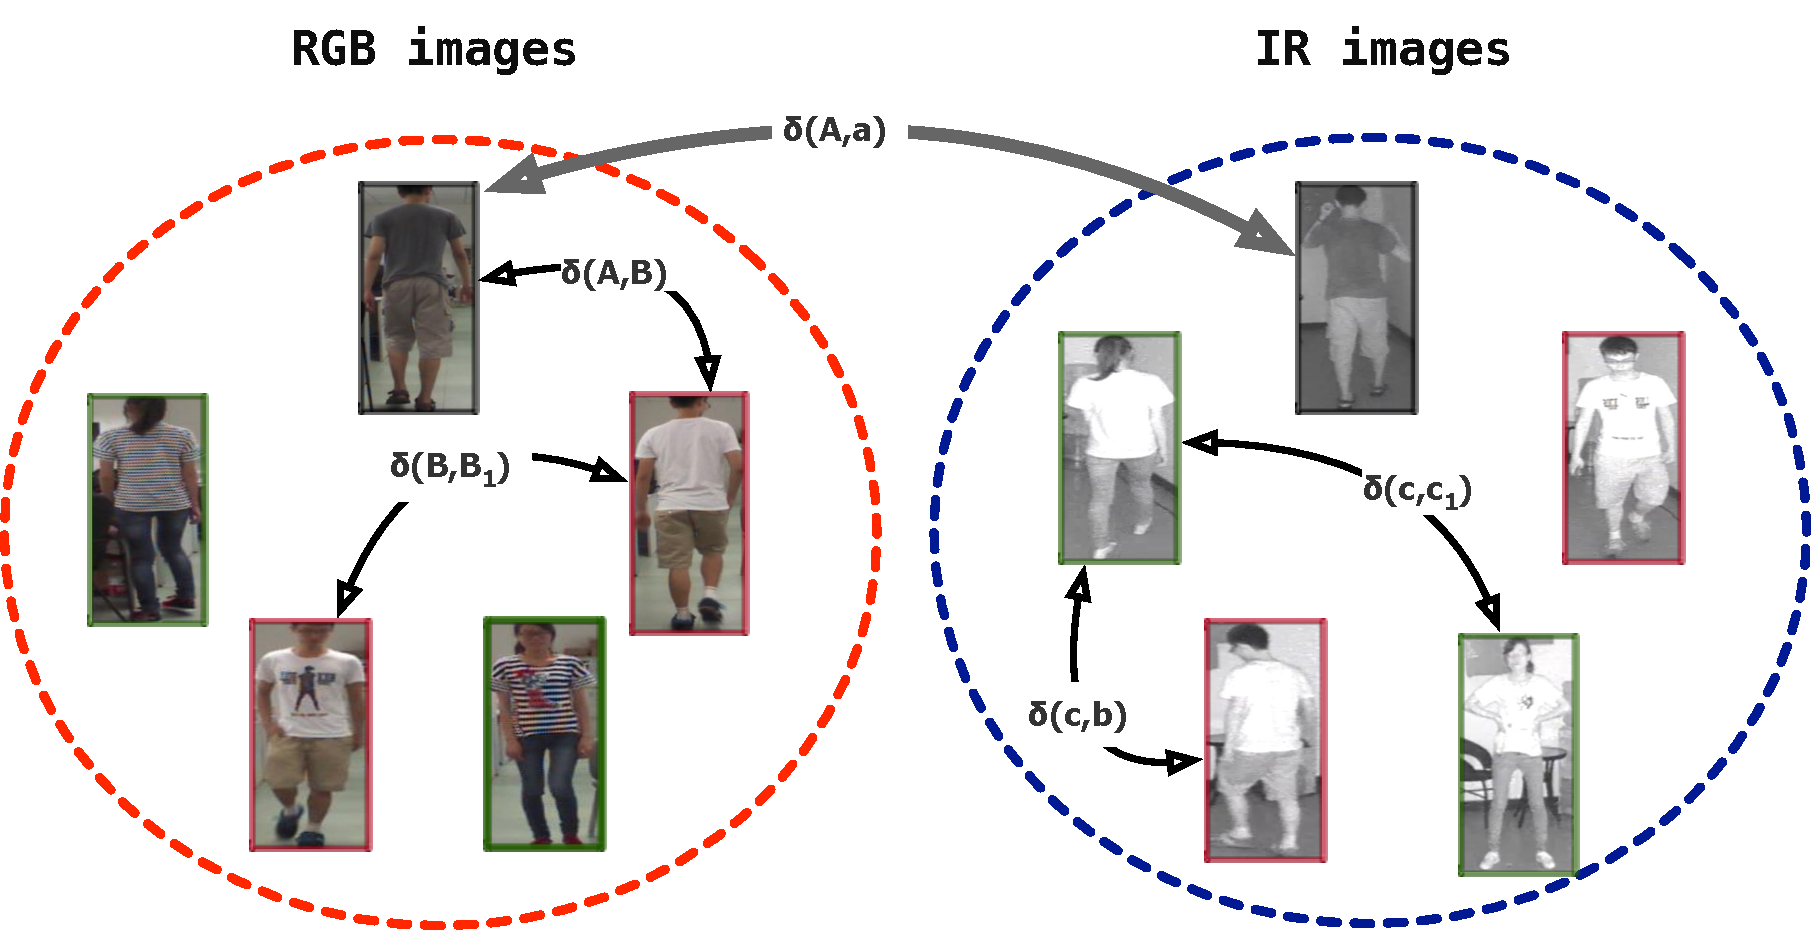
\includegraphics[width=14.5cm]{02/arch1.pdf} \\
    \bicaption[跨模态行人重识别介绍图]
      {跨模态行人重识别难点示意图, 图中展示出来跨模态的变化以及模态内的变化带来的难点。每一张被同色方框围住的图片属于同一个行人。由于模态的差异性以及变化带来的影响, 同一行人的距离 $\delta(A, a)$比不同行人的距离$\delta(A, B)$还大。 同时, 由于模态内的变化存在, 同一行人不同照片的距离 $\delta(c, c_1)$ 也超过了不同行人照片的距离$\delta(c, b)$。}
      {Illustration of the difficulty of VT-REID resulted from the modality discrepancy, cross-modality variation and intra-modality variation. Boxes with the same color denote pictures from the same person. Owing to the crossmodality discrepancy and variation, the intra-person distance$ \delta(A,a)$ is larger than the inter-person distance $\delta(A, B)$. Further, as demonstrated in the right part of the picture, intra-person distance $\delta(c,c_1)$ is larger than $\delta(c,b)$ caused by intra-modality variation.}
   \label{fig:arch1}
\end{figure} 
和传统行人重识别相比, VT-ReID 由于跨模态差异 (Cross-modality Discrepancy)的存在而尤其地具有挑战性, 如图~\ref{fig:arch1}。跨模态的差异一般是由于可见光和热度图成像使用的不同的光谱造成。同时, 如图~\ref{fig:arch1}所示, 由于捕捉行人图像的摄像机角度的差别, 以及行人外表着装等的改变带来的模态内的变化更加剧了跨模态检索的难度。\par
现阶段的跨模态行人重识别方法一般包含两个通用的流程: (1) ``\textbf{特征提取}'' 和 (2)``\textbf{相似度学习}'' 。对于``\textbf{特征提取}'', 现有的算法框架基本基于卷积神经网络例如 AlexNet 或者 ResNet 等来提取特征, 这种简单 CNN 结构的特征提取方法很难保证能提取出充满信息量的特征, 从而对第二阶段的相似度学习带来负面的影响。例如, 来自同一个行人的图片由于着装不同, 光照差异, 姿态不同等差别导致CNN提取的特征截然不同, 导致产生迥异的特征嵌入向量。由于精确的行人检索需要CNN提取的同一行人的特征向量尽量接近, 这也启发了我们基于基础的卷积
\begin{figure}[!htp]
    \centering
    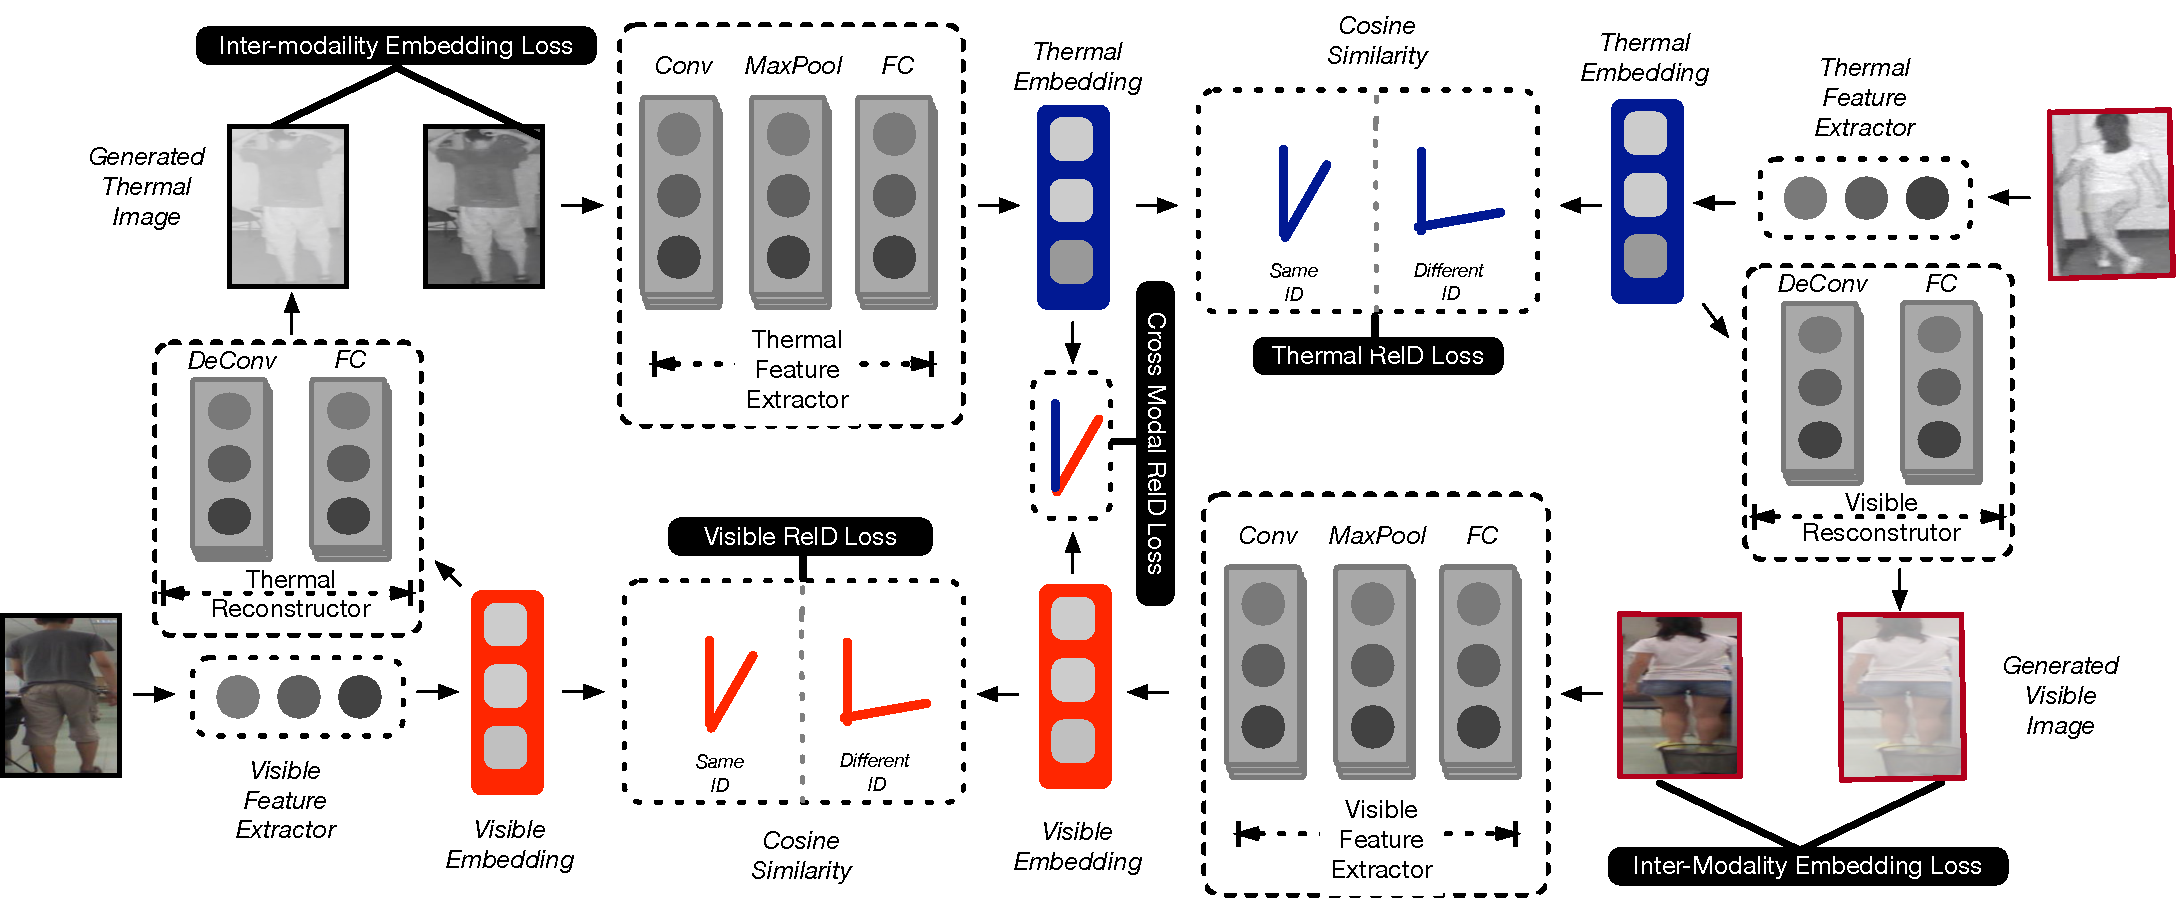
\includegraphics[width=15.0cm]{02/arch.pdf} \\
    \bicaption[跨模态行人重识别MAENet框架示意图]
      {本章提出的跨模态行人重识别MAENet框架的示意图。由图所示, Thermal特征提取器为一个卷积神经网络将从Thermal模态的图片提取特征向量。同样 Visible 特征提取器从Visible模态提取对应特征向量。对应Thermal 和 Visible 重建器从特征向量生成对应Thermal 和 Visible的图片。同时ReID loss是基于贝叶斯的成对损失函数用于跨模态和模态内检索训练。}
      {The framework of the proposed framework- MAENet in this chapter. As illustrated, the fhermal feature fxtractor is a convolutional neural network responsible for extracting feature vector from thermal images. in the same way, the visible feature extractor extracts features from the visible images. The thermal and visible reconstructors are responsible for reconstructing thermal and visible images. The reid losses are devised to perform cross-modal and intra-modal person re-identification.}   
      \label{fig:arch}
\end{figure} 
神经网络设计一个框架来提取对于模态和外表恒定的特征的想法。如图~\ref{fig:arch1}所示, 对于两个绿色框围住的两张来自同一行人的图片, 尽管他们的视觉图像特征截然不同, 但是两张图片中的行人展示出相似的轮廓特征, 这样的轮廓特征便可以帮助我们实现识别同一行人的任务。受这一发现的启发, 本章提出一个全新的框架图 \textbf{MAENet}, 用来完成跨模态的行人重识别任务。我们设计并且实现了一个新的模态和外表恒定编码的网络来提取由不同摄像头不同角度拍摄的同一行人照片的公共的特征。 如图~\ref{fig:arch} 所示, 框架类似于自编码器的架构, 由两个特征提取器 (Visible Feature Extractor 和 Thermal Feature Extractor) 以及两个图像重建器 (Thermal Reconstructor 和 Visible Reconstructor)组成。其中每个图像重建器会从同一行人的在同一模态的图像特征重建图片或者从另一模态的图片的特征重建当前模态的图片。例如, 对于来自同一行人$i$的图片$x_i$, $\hat{x}_i$, $y_i$ 其中 $x_i$ 和 $\hat{x}_i$是来在可见光模态的图片而$y_i$是来自于红外线模态的热度图片。我们的模型将从$x_i$提取的特征恢复成$y_i$图片, 并用L2损失来衡量恢复的优劣。同时也将从$x_i$的图片特征恢复成$\hat{x}_i$的图片, 从而促使模型学习到同一行人在不同的模态不同的外表下的共享的恒定的那一部分特征。
同时, 为了进行相似度学习, 我们设计了两种基于成对训练数据的损失函数来进行跨模态以及单模态的检索训练。本章的主要贡献可以概括为下面的三点:
\begin{enumerate}
    \item 本章提出了一个新型的模态和外表恒定特征编码的框架来提取跨模态和不同外表下的共享的那部分特征用于行人重识别任务。
    \item 本章设计并且推导了基于带权最大似然估计的损失函数用于保留跨模态的相似度以及进行模态内的相似度学习。据我们所知, 这是第一个基于最大似然估计推导应用于跨模态行人重识别的工作。
    \item 本章的算法在多个公共标准数据集上进行了完善的实验, 实验结果表明本章的算法比之前发表的工作具有更加优越的性能, 证实了提出的框架的有效性以及泛化性。
\end{enumerate}

\section{相关工作}
与本章所提出的算法相关的一些工作主要分为两个方面: ``行人重识别'' 和 ``跨模态行人重识别''。 接下来这一小节, 我们着重介绍这些方法的设计和实现以及我们的相关性。
\subsection{行人重识别}
和行人重识别相关的工作可以分成一下两个类别: ``基于手工特征的方法'' 和 ``基于深度学习的方法''。 \par
\textbf{基于手工特征的方法:} 
基于手工特征的核心方法是用人为去设计选取最具有分辨力的图像特征用于后阶段的度量学习~\cite{gray2008viewpoint, hu2013exploring, gheissari2006person, farenzena2010person, ma2012local, cheng2011custom}。Gray 和 Tao 提出~\cite{gray2008viewpoint}使用 AdaBoost 来动态的从色彩和纹理的特征中选取适用于检索的有判别性的特征。Farenzena 等人~\cite{farenzena2010person} 提出一种 Symmetry-Driven Accumulation of Local Features (SDALF)方法, 通过考虑对称性以及非对称性来处理行人图像的视角变化。Ma 等人~\cite{ma2012local} 将局部的描述符转换成 Fisher
Vector 来得到图片的一个全局的特征向量。 Cheng 等人~\cite{cheng2011custom} 基于Pictorial Structure 算法考虑分块的颜色信息来进行行人检索。Liao 等人随后提出了 Local Maximal Occurrence (LOMO), 通过分析纵向局部特征的出现频率, 并且通过最大化出现的频次来获得稳定的特征表示。 同时对于检索需要的度量学习, 通过跨视角的二次判别分析来学习一个子空间, 随后在子空间学习一个QDA的度量函数。LOMO 随后被~\cite{zhang2016learning} 以及~\cite{zhang2016sample} 采用来获取强健的图像表征。Chen~\cite{chen2015mirror} 提出一个基于零填充的特征变换策略来对齐不同视角的特征分布, 这种方法能极大提高现有模型的准确度。 Shi随后~\cite{shi2015transferring} 通过学习中等层次的语义特点例如发型, 鞋子款式 和着装等来获得更加有力的特征表示。 \par
\textbf{基于深度学习的方法:}
与基于手工特征方法不同的是, 基于深度学习的重识别方法使用深度神经网络根据监督信号自动提取图像
特征, 能得到更加有判别力强健的特征表示。基于深度学习的方法由于取得的优异的性能也已经成为了行人重识别的的主流方法。 \par
第一次将深度学习引入行人重识别任务的是~\cite{yi2014deep}和~\cite{li2014deepreid}。2014年, Dong~\cite{yi2014deep} 提出一个基于孪生卷积神经网络的架构直接从输入的图片提取特征, 然后基于二分类损失函数和反向传播优化神经网络。Wei~\cite{li2014deepreid} 等人提出 FPNN 使用一个统一的神经网络同时处理遮挡,背景繁杂等等行人重识别的难题, 并且使用负对数似然 (Negative Log Likelihood)损失函数进行成对的训练。随后, Lin 等人~\cite{wu2016personnet} 通过使用更小的卷积核加深了提取特征的卷积神经网络的深度, 极大的提高了重识别的准确度。Rahul Rama 等人~\cite{varior2016siamese} 将循环神经网络的一个经典架构-长短期记忆网络 (Long Short-term Memory, LSTM) 引入进重识别, 通过LSTM对图片的的分块特征进行序列化的建模来提高得到的图像特征的辨别能力。2018年, Sun 等人~\cite{sun2018beyond} 提出 PCB, 通过一个基于分块的卷积神经网络来提取细粒度的特征以及一个改进的分块池化策略 (RPP)来生成分块的特征向量, 最后通过在每个局部向量上进行分类损失计算来训练模型进行重识别检索任务。Feng~等人~\cite{feng2018learning} 提出在特征提取的阶段引入摄像视角的信息来减缓类内的变化带来的影响。Yu ~\cite{yu2019unsupervised} 探索了用无标签监督的方法进行行人重识别的可能性。Liu 等人~\cite{liu2019deep} 为了提高重识别算法在现实生活中的应用, 提出了使用human-in-the-loop的强化学习来收集数据不断的更新模型。 这样可以最大限度的减少人工标注数据的开销以及提高重识别模型的性能。随后, Eom 等人~\cite{eom2019learning}基于生成对抗网络提出 IS-GAN 用来对行人的表征解耦, 将行人的身份相关的特征从与身份无关的特征中解耦出来。尽管这些方法在许多的行人重识别数据集上获得了不错的性能表现, 他们都是专注解决单可见光模态的行人检索, 并不能直接被应用到跨模态的行人重识别任务中。
\subsection{跨模态行人重识别}
对于跨模态的行人重识别, 研究人员已经研究了 RGB-Depth~\cite{haque2016recurrent, munaro20143d, wu2017robust},  Text-Image ~\cite{li2017identity,li2017person,ye2015specific, yin2017adversarial}。本章研究的跨模态行人重识别主要指的Visible-Thermal 重识别 (VT-ReID)。 2017年, Wu 等人~\cite{wu2017rgb}第一次提出VT-ReID的概念, 并且提出了一个基于零填充的网络结构来学习公共的特征。2018年, Ye 等人~\cite{ye2018visible} 提出使用双流卷积神经网络来将两个模态的图片映射到可以比较的同一特征空间
\begin{figure}[!htp]
    \centering
    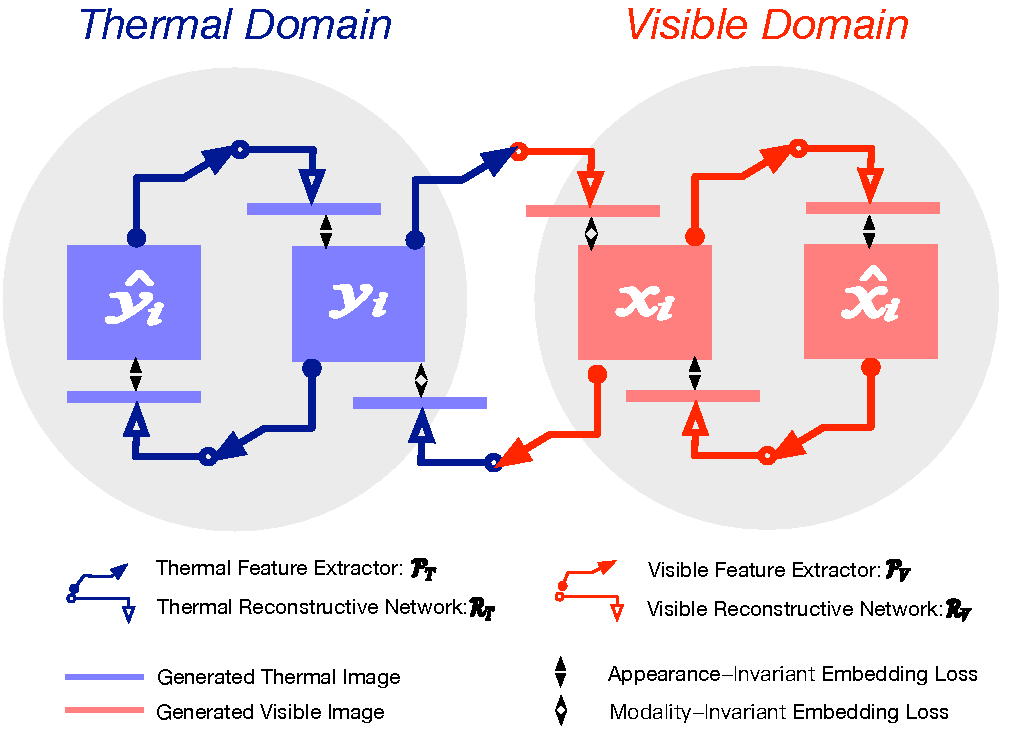
\includegraphics[width=12.0cm]{02/arch2.pdf} \\
    \bicaption[模态和外表恒定重建编码架构图]
      {模态和外表恒定重建编码的基础架构图。红色代表visible模态, 蓝色代表thermal模态。$x_i$ 和 $\hat{x}_i$是来自visible模态的同一行人图片, $y_i$和 $\hat{y}_i$是来自thermal模态的同一行人照片。由图所示, 使用了两种不同的损失函数来学习模态内外表恒定的特征以及跨模态恒定的特征。}
      {The illustration of modality and apperance invariant embedding framework. Red color represents the visible modality and blue color stands for the thermal modality. $x_i$ and $\hat{x}_i$ are person images from the visible modality while $y_i$ and $\hat{y}_i$ are from the thermal modality. Two embedding loss are enforced to learn  apperance-invariant and modality-invariant feature embeddings.}   
      \label{fig:arch2}
\end{figure} 

中。 同时基于排序损失, 作者提出了一个 Dual-Constrained Top-Ranking 的损失函数来减轻跨模态变化以及模态内变化带来的影响。随后, 作者改进了基础的双流神经网络, 在两个卷积神经网络后层的全连接网络共享权重。同时, 作者提出了一个二阶段学习策略, 第一阶段进行特征学习, 第二阶段进行度量学习, 通过一个分层次的跨模态匹配模型优化模态特有的以及模态共享的特征。2019年, Hao等人~\cite{hao2019dual} 基于 PCB 模型设计双流 PCB 主干结构, 在特征分布的层面对齐每一个分块的特征。随后, 他又提出一个新型的算法 HSME~\cite{hao2019hsme} 通过将特征映射到超球面, 然后在超球面进行特征嵌入学习。Ye 随后提出~\cite{ye2019modality}基于双流神经网络的模态感知的协同学习方法, 同时可以在特征层面以及分类器层面解决模态差异带来的影响。特征层面是通过双流神经网络来映射到相同的空间减轻模态差异的影响。在分类器层面则是通过两个模态特有的分类起来捕获模态特定的信息。然而, 前面提到的大多数的算法主要集中关注在后一阶段的度量学习来减轻模态差异以及模态内变化带来的影响, 忽略了在网络结构层面直接解耦提取出最适用于跨模态检索的有辨别性特征的重要性。

\section{MAENet}
\subsection{本章主要符号定义以及问题定义}
在整章中, 我们使用书法大写字母 (calligraphic uppercase), 例如 $\mathcal{X}$ 来表示映射函数。本章使用粗体大写字母 (Bold-face uppercase), 例如 $\mathbf{B}$ 来代表集合以及粗体小写字母来代表向量, 如 $\mathbf{b}$。 $U$代表向量空间。 \par
\textbf{问题定义:} 假设 $\mathbf{X}=\{k\}_{i=1}^N=\mathbf{V} \cup \mathbf{T}$ 是一个包含 $N$ 个训练样本的集合, 其中包含了来自visible 模态的行人照片$\mathbf{V}$以及thermal 模态的行人照片$\mathbf{T}$。$I_{k_i} = i$是一个特征函数将图片映射到它的索引。$\mathcal{S}: N * N \rightarrow\{0,1\}$是一个相似性映射函数。 $\mathcal{S}_{ij} = 1$ 如果 $k_i$ 和 $ k_j$ 图片是属于来自同一个人的照片。  $\mathcal{S}_{ij} = 0$ 如果 $k_i$ 和 $ k_j$ 图片是属于来自不同人的照片。 $\mathbf{P}=\left\{\left\{k_p, k_q: S_{p q}=1\right\}: p, q \in N\right\}$ 是一个包含了所有同一个行人图片对的集合。监督VT-ReID的目标就学习两个特征映射函数 $\mathcal{F}_V: \mathbf{V} \rightarrow \mathbf{U}$ 和 $\mathcal{F}_T: \mathbf{T} \rightarrow \mathbf{U}$, 其中需要满足: 给定任意的在检索图片集中的一张行人照片, 例如来自visible 模态的检索照片 $\mathbf{V}^{\prime} \subset \mathbf{V}$ 以及一个数据库 $\mathrm{T}^{\prime} \subset \mathrm{T}$, 找到 图片 $k \in \mathbf{T}^{\prime}$ 其中 $S_{I_v I_k}=1$。\par
本章提出一个基于深度学习的框架用于VT-ReID, 这个框架集成了增强的特征学习以及度量学习, 并且基于一种端到端的优化方法进行直接优化, 整个框架图如图~\ref{fig:arch}。
\subsection{混合双流特征提取架构}
混合双流特征提取架构如架构图~\ref{fig:arch}所示, 其包含两个模态特定的卷积神经网络$\mathcal{F}_V$ 和 $\mathcal{F}_T$ 来提取visible和thermal模态的图片特征。两个特征提取卷积神经网络的结构完全相同, 都是基于Resnet-50~\cite{he2016deep}。同时, 额外的全连接层添加在Resnet-50后来将特征映射到一个两个模态共享的特征空间。值得注意的是, 额外添加的两个全连接层共享参数, 以便于学习到模态共有的特征信息。
\subsection{模态和外表恒定的重建编码}
为了进一步保证上述从两个模态数据中提取的特征向量包括必要的有判别性的信息, 我们思考在特征层面增加额外的约束条件的可能性。受~\cite{cao2016correlation}使用基于自编码器的网络架构来提取跨模态关联的启发, 我们设计了一个新的网络结构如图~\ref{fig:arch2}所示。网络除了基础的双流卷积神经网络, 即thermal特征提取器$\mathcal{F}_T$和visible特征提取器$\mathcal{F}_V$之外, 还包含两个特征重建神经网络, 即thermal重建网络$\mathcal{R}_T$以及visible重建网络$\mathcal{R}_V$。为了生成模态恒定特征的损失函数可以由如下的公式表示: 
\begin{equation}
  L_{M I}=\sum_{\mathbf{Q} \in \mathbf{P}} \sum_{x_i, y_i \in \mathbf{Q}}\left(\left\|x_i-\mathcal{R}_V\left(\mathcal{F}_T\left(y_i\right)\right)\right\|_2^2+\left\|y_i-\mathcal{R}_T\left(\mathcal{F}_V\left(x_i\right)\right)\right\|_2^2\right).
  \label{eq:MI_loss}
\end{equation} 
其中$\mathcal{R}_V$和$\mathcal{R}_T$是基于反卷积的深度神经网络, 将特征向量重建成对应的visible模态的图片以及thermal模态的图片。$\mathcal{F}_V$和$\mathcal{F}_T$则是两个深度卷积神经网络从输入的图片提取特征并且映射成一个低维的特征向量。$x_i \in \mathbf{V}$ 是来自visible模态的图片, 而$y_i \in \mathbf{T}$是来自thermal模态的图片。同时, $x_i$ 和 $y_i$ 是来自同一行人$i$的两张属于不同模态的图片。通过降低此跨模态重建的误差$L_{M I}$, 从一个模态图片提取的特征向量则会学习到模态不变的特征以便于恢复成对应另一模态的图片。由于VT-ReID同时还受到模态内变化 (Intra-modality Variation) 的影响, 本章另外提出了一个外表恒定的损失函数来促使模型捕捉到在一个模态内同一行人在不同的摄像视角, 着装, 姿态等情况下的共享的信息, 如图~\ref{fig:arch2}右所示。外表恒定损失函数如下所示:
\begin{equation}
  \begin{aligned}
  L_{AI} = \sum_{\mathbf{Q} \in \mathbf{P}}\sum_{x_i,\hat{x_i},y_i,\hat{y_i} \in \mathbf{Q}}(&||x_i - \mathcal{R}_V(\mathcal{F}_V(\hat{x_i}))||_2^2+
      ||\hat{x_i} - \mathcal{R}_V(\mathcal{F}_V(x_i))||_2^2  \\
      +&||y_i - \mathcal{R}_T(\mathcal{F}_T(\hat{y_i}))||_2^2+ 
      ||\hat{y_i} -\mathcal{R}_T(\mathcal{F}_T(y_i))||_2^2).
  \end{aligned}
  \label{eq:AI_loss}
  \end{equation}
  其中$L_{A I}$表示两个模态的模态内外表恒定损失函数的集合, 其中$\hat{x}_i \in \mathbf{V}$ 且 $\hat{y}_i \in \mathbf{T}$ 是和$x_i$, $y_i$分别同模态同一个行人的不同照片。通过最小化损失函数$L_{A I}$, 特征提取器 $\mathcal{F}_T$或者$\mathcal{F}_V$会学习从同一个行人的不同照片中学习到对外观恒定的一部分特征, 例如行人的轮廓或者其他可以有助于识别定位的特征。我们将完整的重建损失定义为以上两种损失函数之和, 如下所示:
  \begin{equation}
    L_{RE} = L_{MI} +L_{AI}
    \label{eq:re}
\end{equation}
通过最小化~\ref{eq:re}这个损失函数, 特征学习神经网络$\mathcal{F}_T$和$\mathcal{F}_V$ 可以同时生成对模态和外观都不变的特征向量, 从而极大的提高后续检索任务的性能。
\subsubsection{基于成对关联的相似度学习}
为了有效的进行跨模态行人重识别任务, 以及支持单模态重识别的操作, 假设我们有两张来自于同一行人的照片$x_i$和$x_j$, 则它们两相对应的特征向量$\mathbf{x}_i$ 和 $\mathbf{x}_j$ 在特征空间上应该比较接近, 即有比较短的欧式距离, 反之亦然。为了更好的保证这一点, 我们设计了一个目标函数直接包含了三种损失函数: (1) 跨模态的成对检索损失函数 (2)模态内的成对检索损失函数 (3)分类损失函数。\par
假设, 我们有一个训练数据集$\mathbf{X}= \{x_i\}^B_{i=1}\cup\{y_j\}^B_{j=1}, B < N$, 我们可以通过对应的特征提取器$\mathcal{F}_T$ 和  $\mathcal{F}_V$得到对应的特征向量 $\mathbf{H} = \{h_i^V\}_{i=1}^B\cup\{h_j^T\}^B_{j=1}$, 其中 $h_i^V = \mathcal{F}_V(x_i)$ $x_i$是来自visible的图片。而对于来自thermal模态的图片$y_i$, 则有 $h_j^T = \mathcal{F}_T(y_j)$。相似性标签写作 $s^{mn}_{ij} = S_{I_{k_i^m}~I_{k_j^n}}$, 其中 $m$ 和 $n$代表模态。$I_{k^m_i}$表示第$i_{th}$章图片在模态$m$的数据集合中的索引。通常说来, $s^{VT}_{ij}=1$意味着第$i_{ith}$和第$j_{th}$组成的图片对 $(k^V_i,k^T_j)$ 分别来自visible和thermal模态, 并且它们属于同一个行人的不同照片。基于以上定义, 其似然函数可以正式描述为:
\begin{equation}
  p(s^{mn}_{ij}|h_i^m,h_j^n) = \sigma{(d(h_i^m,h_j^n))}^{s^{mn}_{ij}}(1 - \sigma{(d(h_i^m,h_j^n))})^{(1-s^{mn}_{ij})} \label{con:conditional} \\
\end{equation}
其中 $d(h_i^m,h_j^n) = \cos{(h_i^m,h_j^n)}$ 是 $h_i^m$和 $h_j^n$的余弦距离。同时, $\sigma(x) = \frac{1}{1+e^{-x}}$ 是sigmoid激活函数。 $ p(s^{mn}_{ij}|h_i^m,h_j^n)$表示在得到两个特征向量$h_i^m$ and $h_j^n$后 $s^{mn}_{ij}$ 的条件概率。同时, 我们另外定义了一个权重参数 $w_{ij}^{mn}$ 来解决数据不平衡的问题~\cite{cao2018deep}:
\begin{equation}
  w^{mn}_{ij} = 
  \begin{cases}
  |\mathbf{S}|/|\mathbf{S}^{mn}_1|, &s^{mn}_{ij}=1\\
  |\mathbf{S}|/|\mathbf{S}^{mn}_0|, &s^{mn}_{ij}=0 \\
  \end{cases}
\end{equation}
其中$\mathbf{S}^{mn}_1 = \{(i,j): s^{mn}_{ij}=1\}$是一个图片对的集合, 其中每个图片对都属于同一个行人。 $\mathbf{S}^{mn}_0 = \{(i,j): s^{mn}_{ij}=0\}$ 则是一个图片对的集合, 其中每个图片对包含的图片来自不同的行人。\par
接下来, 我们会展示跨模态行人重识别损失函数的推导过程。我们基于最大似然估计 (Maximum Likelihood Estimation, MLE) 来推导。用来进行跨模态检索的带权的最大似然估计的损失函数$L_{Inter}$ 如下式~\ref{eq:inter}所示:
\begin{equation}
  \begin{aligned}
     L_{Inter} &= -\log{ p(\mathbf{S}|\mathbf{H})} 
      =  -\sum_{i, j}w^{VT}_{ij}\log{p(s^{VT}_{ij}|h_i^V,h_j^T)} \\
      &= -\sum_{i,j}w^{VT}_{ij}(s^{VT}_{ij}d(h_i^V,h_j^T)-log(1+e^{d(h_i^V,h_j^T)}))
 \end{aligned}
 \label{eq:inter}
  \end{equation}
非常明显, 通过优化~\ref{eq:inter}, 相同图片对的余弦相似度会增加, 不同图片对的特征向量的余弦相似度会降低。但是由于$L_{Inter}$并没有考虑到单模态内的检索问题, 也没用考虑到模态内变化的影响, 因此, 自然我们需要针对visible模态和thermal模态设计两个模态内的重识别损失函数。\par
对于thermal模态的图片, 训练的图片对 $(y_i, y_j)$都是来自thermal模态的行人照片。和跨模态的重识别损失函数类比可得到模态内重识别损失函数的构造:
\begin{equation}
  L_{Intra\_Thermal} = -\sum_{i,j}w^{TT}_{ij}(s^{TT}_{ij}d(h_i^T,h_j^T)-log(1+e^{d(h_i^T,h_j^T)}))
  \label{eq:intrathermal}
\end{equation}
同样的, 我们也可以用相同的方式来推导出在visible模态的成对重识别损失函数:
\begin{equation}
  L_{Intra\_Visible} = -\sum_{i,j}w^{VV}_{ij}(s^{VV}_{ij}d(h_i^V,h_j^V)-log(1+e^{d(h_i^V,h_j^V)}))
  \label{eq:intravisible}
\end{equation}
这样, 模态内的重识别损失函数$L_{Intra}$则可视为visible和thermal的两个损失函数之和:
\begin{equation}
  L_{Intra} = L_{Intra\_Visible} + L_{Intra\_Thermal}
\label{eq:Intra}
\end{equation}
为了进一步提高学习到的表征的可辨别性, 如论文~\cite{ye2018visible}所示, 我们进一步继承了一个身份损失函数 (Identity Loss), 实际上也是一个分类损失函数, 将每一个行人当作一个类别, 并且使用softmax交叉熵来进行监督分类器的学习, 其可用正式的公式表示为:
\begin{equation}
  L_{\text {Identity}}=-\sum_{i=1}^N \log \frac{e^{\mathbf{W}_{y_i}^T \mathbf{h}_{\mathrm{i}}}}{\sum_{k=1}^C e^{\mathbf{W}_k^T \mathbf{h}_{\mathrm{i}}}}.
  \label{eq:identity}
\end{equation} 
其中 $\mathbf{W}_k$是对于第$k$个行人的权重向量, $N$是每个batch的图片数, 照片中的类别总数也就是行人的个数为$C$。值得注意的是, 我们分别对每个模态的特征进行分类学习。通过这种方式, 学习到的特征可以更多的保留与行人相关的特征, 也一定程度减轻了模态内变化的影响。\par
全面的训练目标函数可以视作上述所有的损失函数之和, 即:
\begin{equation}
  L_{total} = L_{Inter}+\lambda_1L_{Intra}+\lambda_2L_{Identity} + \lambda_3L_{RE}
\label{eq:total}
\end{equation}
其中, $\lambda_1$,~$\lambda_2$,~和 $\lambda_3$ 是三个预先设定好的系数用来控制各个不同损失函数在总体训练目标中的影响。
\subsection{优化算法}
本章的优化整个框架的算法如算法~\ref{algo:main}所示。我们有一个训练数据集$\mathbf{X}$ 以及对应的相似性标签$\mathbf{S}$。最初的学习率设置为$\alpha$, 并且我们分别设置三个超参数$\lambda_1, \lambda_2, \lambda_3$来平衡各个损失函数在公式~\ref{eq:total}中的影响。最大的迭代轮数设置为$T$。 首先, 我们将$\theta_{V}$和$\theta_{T}$用在ImageNet上预训练好的参数进行初始化。 然后, 我们基于Xavier初始化随机初始化$\theta_{RV}$和$\theta_{RT}$。迭代轮数计数器$t$被设置为 $0$。 \par
在模型未收敛并且迭代次数$t$比最大迭代次数$T$小时, 我们进行下列操作。首先, 我们将$t$增加$1$。然后, 根据采样策略从输入的数据集中$\mathbf{X}$随机采样一个batch的数据。将数据输入模型, 计算各个部分损失函数的数值。
随后, 计算梯度并且通过反向传播得到各个参数对应的梯度。最后根据梯度更新模型的参数。\par
以上操作循环进行直到模型收敛或者迭代次数超过设定的最大值。


\begin{algorithm}
  \caption{MAENet框架的优化算法}\label{algo:main}
  \KwData{训练图片集 $\mathbf{X}$,~相似性标签 $\mathcal{S}$, ~学习率 $\alpha$ and 损失函数系数 $\lambda_1$, $\lambda_2$, $\lambda_3$~ 最大迭代轮数$T$}
  \KwResult{优化的网络结构参数 $\theta_V$,~$\theta_T$, $\theta_{RV}$,~$\theta_{RT}$;}
  $t \leftarrow 0$\;
  $\theta_V \leftarrow ImageNet预训练参数$  \; 
  $\theta_T \leftarrow ImageNet预训练参数$  \; 
  $\theta_{RV} \leftarrow \textbf{Xavier}(\theta_{RV})$  \; 
  $\theta_{RT} \leftarrow \textbf{Xavier}(\theta_{RT})$  \; 
  \While{未收敛 \textbf{and} $t < T$}
  {
    $t \leftarrow t +1 $\;
   从 $\mathbf{X}$ 中采样 $Q_1, Q_2 \in \mathbf{P}, Q_1 \cap Q_2 = \emptyset $ 来得到$x_i$,~$\hat{x}_i$,~$y_i$,~$\hat{y}_i$ $\in  Q_1$, $x_j$,~$\hat{x_j}$,~${y_j}$,~$\hat{y_j} \in Q_2$ \;
   用 ~$\mathcal{F}_V(\bullet;\theta_V)$,~$\mathcal{F}_T(\bullet;\theta_T)$,~$\mathcal{R}_V(\bullet;\theta_{RV})$,~$\mathcal{R}_T(\bullet;\theta_{RT})$ 通过 Eq. \ref{eq:MI_loss}, \ref{eq:AI_loss}, \ref{eq:re} 计算 $L_{RE}$  \;
   对于 $p \in \{i, j\},~$,$h_p^V = \mathcal{F}_V(x_p;\theta_V)$, $h_p^T = \mathcal{F}_T(y_p;\theta_T)$ \;
   通过 Eq.~\ref{eq:Intra} 计算 $L_{Inter}$ \;
   通过 Eq.~\ref{eq:intrathermal} 计算 $L_{Intra\_Thermal}$ \;
   通过 Eq.~\ref{eq:intravisible} 计算 $L_{Intra\_Visible}$ \;
   通过 Eq.~\ref{eq:identity} 计算 $L_{Identity}$ \;
   $L_{total} \leftarrow L_{Inter} + \lambda_1 (L_{Intra\_Thermal} + Intra\_Visible) + \lambda_2 (L_{Identity}) + \lambda_3 (L_{RE}) $ \;
   反向传播得到 $\nabla_{\theta_*}$~$*\in \{V, T, RV, RT\}$ \;
  $\theta_* \leftarrow \alpha ( \theta_* - \nabla_{\theta_*}) $ \;
  }
 
  \end{algorithm}

\section{实验结果与分析}
本章进行了充足广泛的实验来验证我们提出的模型结构的有效性。在接下来的段落中, 本小节先介绍了数据集的设置以及基本信息, 然后阐述了本文使用的评估标准以及模型的实现细节。 随后, 本小节详细展示了本章提出的算法在各个标准数据集上取得的结果以及与先进的其他算法的比较细节来证明模型的性能。最后, 本小节展示了文章提出的消融实验来证明模型的各个组成部分的有效性。
\subsection{数据集}
本节的实验采取了两个标准的跨模态VT-ReID任务中数据集进行训练与测试。为了实现与现有的先进方法比较的公平公正, 我们采取标准的训练集和测试集的划分方法来进行对比实验。两个数据集的具体信息如下:
\begin{enumerate}
  \item \textbf{RegDB}~\cite{nguyen2017person} 是通过双摄像头系统的监控摄像机收集, 一共包含 $412$ 个行人。 对于每一个行人都包含十张来自visible模态的不同照片以及十张来自thermal模态的不同的照片。本小节采取~\cite{ye2018hierarchical}的实验方法, 将数据集随机分成两半, 一半组成训练集, 对应另一半是测试集。对于测试, 来自一个模态的所有图片当成检索图片, 对应另一个模态所有图片组成了被检索的数据库。 
  \item \textbf{SYSU-MM01}~\cite{wu2017rgb} 是一个由六个摄像机收集的大规模检索数据集, 包括4个可见光摄像头和2个红外摄像头。这个数据集由于包含室内和室外两种场景而显得更具有挑战性。 数据集一共包含$491$个行人, 每个行人至少包括两个摄像头拍摄的照片。 数据集标准测试有两个模式 \textit{indoor search} 和 \textit{all search}。对于 \textit{indoor search}模式, 即排除了在户外的摄像头拍摄的行人照片。由于 \textit{all search}显然更具有挑战性, 本节遵循 Ye et al ~\cite{ye2018visible} 主要采取 \textit{single-shot all search}的场景。 其中, 训练数据集包含$395$个行人, $22,258$ 张visible的图片以及$11,909$张thermal图片。 而测试数据集则包含$96$个行人, $3,803$张thermal的照片以及 $301$张visible的图片。在没有特殊说明的情况下, 均是使用thermal的图片进行检索, visible图片作为被检索的数据库。
\end{enumerate}
\subsection{评价指标}
我们采取平均准确率均值 (Mean Average precision, mAP) 以及累积匹配曲线 (Cumulative Matching Characteristic, CMC) 来评估方法的性能。其中 \textbf{mAP}的计算如下
\begin{equation}
   \textbf{mAP} = \frac{1}{n} \sum_{k=1}^{k= N} \textbf{AP}_k
\end{equation}
其中$N$是查询的图片总数。由此式可知, $mAP$则为每张图片的平均准确率的平均值。
\subsection{模型实现细节}
本章算法通过Pytorch 框架编码实现, 所有的实验是在一台4个Intel Core i7-4790K CPU核以及NVIDIA GeForce 1080Ti显卡上进行。全连接层后的输出维度设置为 2048, 两个数据集的 batch 大小设置为64。 Dropout率设置为 0.5。对于所有输入的图片, 首先会被缩放至 $256 \times 256$ 的大小, 随后会被随机裁剪成 $224 \times 224$的大小以便于输入进神经网络。在训练的阶段, 随机裁剪和随机水平反转被使用来进行数据增强以防止过拟合, 在测试阶段的话, 则使用中心裁剪。 超参数$\lambda_1$, $\lambda_2$和 $\lambda_3$均被设置成 $0.5$。本章采取 Momentum 优化器来进行优化神经网络, momentum设置为 $0.9$。 初使的学习速率设置为 $1e-3$。训练的最大轮数设置为$50000$。


\begin{table}[!htpb]
  %% \centering % not needed
  \bicaption{各个先进的算法在Visible到Thermal的跨模态重识别在RegDB数据集上的测试结果}{Vsible-to-Thermal Test Results of State of The Art Methods on RegDB}
  \centering
  \begin{tabular}{cccccc}
     \\ \hline
  \multicolumn{2}{l|}{Methods} & r=1 &r=10 & r=20 & mAP   \\\hline
  
  \multicolumn{2}{l|}{HOG} & 13.49 & 33.22 & 43.66 & 10.31  \\
  \multicolumn{2}{l|}{MLBP} &  2.02& 7.33 & 10.90 & 6.77  \\
  \multicolumn{2}{l|}{LOMO\cite{liao2015person}} &  0.85& 2.47 & 4.10 & 2.28  \\
  \multicolumn{2}{l|}{GSM\cite{lin2016cross}} &  17.28& 34.47 & 45.26 & 15.06  \\

  \hline
  \hline
  \multicolumn{2}{l|}{SVDNet\cite{sun2017svdnet}} &  17.24& 34.12 & 44.51 & 19.04  \\
  \multicolumn{2}{l|}{PCB\cite{sun2018beyond}} & 18.32& 36.42 & 46.51& 20.13   \\ 
  \hline
  \hline
  \multicolumn{2}{l|}{TONE\cite{ye2018hierarchical}} &  16.87& 34.03 & 44.10 & 14.92  \\
  \multicolumn{2}{l|}{TONE + XQDA} &  21.94 & 45.05 & 55.73 & 21.80  \\
  \multicolumn{2}{l|}{TONE + MLAPG} &  17.82 & 40.29 & 49.73 & 18.03  \\
  \multicolumn{2}{l|}{TONE + SCDL} &  8.06 & 22.09 & 28.89 & 10.03  \\
  \multicolumn{2}{l|}{TONE + rCDL} &  9.47 & 22.96 & 29.42 & 10.26  \\
  \multicolumn{2}{l|}{TONE+HCML }& 24.44 & 47.53 & 56.78 & 20.80 \\
  \multicolumn{2}{l|}{Zero-Padding\cite{wu2017rgb} }& 17.75 &34.21 & 44.35 & 18.90  \\
  \multicolumn{2}{l|}{cmGAN\cite{dai2018cross} }& - & - & - & -  \\
  \multicolumn{2}{l|}{BDTR (ResNet50)\cite{ye2018visible} }& \textcolor{blue}{30.56} & \textcolor{blue}{54.62} & \textcolor{blue}{65.42} & \textcolor{blue}{32.45}  \\
  \hline
  \hline
   \multicolumn{2}{l|}{\textcolor{red}{MAENet} (ResNet50) }&\textcolor{red}{\textbf{44.32}} & \textcolor{red}{\textbf{63.98}} & \textcolor{red}{\textbf{72.67}} & \textcolor{red}{\textbf{45.55}} \\
   \hline
   \hline
  \end{tabular}
  \label{table:visiblethermalRegdb}
\end{table}
\subsection{与其他先进的方法在标准数据集上的结果比较}
我们与解决VT-ReID的先进算法模型在标准数据集上进行性能。具体地, 我们包括了几种基于深度学习的最先进的模型进行仔细的分析研究: \textbf{TONE+HCML}~\cite{ye2018hierarchical}, \textbf{cmGAN}~\cite{dai2018cross}, \textbf{Zero-Padding}~\cite{wu2017rgb}和 \textbf{BDTR}~\cite{ye2019bi}。我们也包括了几种其他的方法, 大部分其他算法的性能来自于~\cite{ye2019bi}。 选择进行比较的算法可以主要分成两类: 基于特征提取的方法 (\textbf{HOG}, \textbf{MLBP}, \textbf{LOMO}~\cite{liao2015person}), 基于匹配模型的方法 (\textbf{XQDA}, \textbf{GSM}~\cite{lin2016cross}, , \textbf{SCDL}~\cite{wang2012semi}, \textbf{rCDL}~\cite{huang2013coupled}, \textbf{MLAPG}~\cite{liao2015efficient})。我们额外加入两个在单模态行人重识别上的先进算法 \textbf{SVDNet}~\cite{sun2017svdnet} 和 \textbf{PCB}~\cite{sun2018beyond} 进行比较。\par
如表格~\ref{table:visiblethermalRegdb} 以及表格~\ref{table:visiblethermalsysu}所示, 本章提出的模型\textbf{MAENet}在 \textbf{RegDB} 和 \textbf{SYSU-MM01}数据集上与现有的先进算法相比较均取得了较大的性能提升。 很明显, 在\textbf{RegDB} 数据集上, 本章的算法比第二先进的算法\textbf{BDTR}在提高了 $13.1 \%$
的\textbf{mAP}, 在$Rank-1$准确度上提高了接近$13.8$。 而在~\textbf{SYSU-MM01} 数据集上 \textit{single-shot all search}场景下, \textbf{MAENet} 也取得了非常优秀的性能表现, 比\textbf{BDTR}提高了 $13.25 \%$ \textbf{mAP}。

\begin{table}[!htpb]
  %% \centering % not needed
  \bicaption{各个先进的算法在Visible到Thermal的跨模态重识别在SYSU-MM01数据集上的测试结果}{Vsible-to-Thermal Test Results of State of The Art Methods on SYSU-MM01}
  \centering
  \begin{tabular}{cccccc}
     \\ \hline
  \multicolumn{2}{l|}{Methods} & r=1 &r=10 & r=20 & mAP   \\\hline
  
  \multicolumn{2}{l|}{HOG} & 2.77 & 18.24 & 31.91 & 4.24  \\
  \multicolumn{2}{l|}{MLBP} & 2.12 & 16.23 & 28.32 & 3.86  \\
  \multicolumn{2}{l|}{LOMO\cite{liao2015person}} &  1.75 & 14.14 & 26.63 & 3.48 \\
  \multicolumn{2}{l|}{GSM\cite{lin2016cross}} &  5.29 & 33.71 & 52.95 & 8.00  \\

  \hline
  \hline
  \multicolumn{2}{l|}{SVDNet\cite{sun2017svdnet}} & 14.64 & 53.28 & 64.24 & 15.17  \\
  \multicolumn{2}{l|}{PCB\cite{sun2018beyond}} & 16.43 & 54.06 & 65.24 & 16.26  \\ 
  \hline
  \hline
  \multicolumn{2}{l|}{TONE\cite{ye2018hierarchical}} &  12.52 & 50.72 & 68.60 & 14.42  \\
  \multicolumn{2}{l|}{TONE + XQDA} &  14.01 & 52.78 & 69.06 & 15.97  \\
  \multicolumn{2}{l|}{TONE + MLAPG} &  12.43 & 50.64 & 68.72 & 14.61  \\
  \multicolumn{2}{l|}{TONE + SCDL} &  6.58 & 35.62 & 56.32 & 10.32  \\
  \multicolumn{2}{l|}{TONE + rCDL} &  7.02 & 37.31 & 57.64 & 10.46  \\
  \multicolumn{2}{l|}{TONE+HCML }& 14.32 & 53.16 & 69.17 & 16.16 \\
  \multicolumn{2}{l|}{Zero-Padding\cite{wu2017rgb} }& 14.80 & 54.12 & 71.33 & 15.95  \\
  \multicolumn{2}{l|}{cmGAN\cite{dai2018cross} }& 26.97 & 67.51 & 80.56 & 27.80  \\
  \multicolumn{2}{l|}{BDTR (ResNet50)\cite{ye2018visible} }& \textcolor{blue}{20.84} & \textcolor{blue}{63.81} & \textcolor{blue}{79.14} & \textcolor{blue}{22.86}  \\
  \hline
  \hline
   \multicolumn{2}{l|}{\textcolor{red}{MAENet} (ResNet50) }&\textcolor{red}{\textbf{29.79}} & \textcolor{red}{\textbf{77.24}} & \textcolor{red}{\textbf{89.87}} & \textcolor{red}{\textbf{36.11}} \\
   \hline
   \hline
  \end{tabular}
  \label{table:visiblethermalsysu}
\end{table}
在 $Rank-1$准确度上也提高了 $8.95 \%$。 同时由表~\ref{table:visiblethermalRegdb}和表~\ref{table:visiblethermalsysu}可知, 传统的单模态的行人重识别算法例如\textbf{PCB} 和 \textbf{SVDNet}并不能取得令人满意的结果, 尽管这两个算法在单模态检索的数据集上表现优异。主要原因是单模态的行人重识别算法没有考虑进来两个不同模态的差异 (Modality Discrepancy), 并不能充足的对齐两个不同模态的特征。而我们的方法由于采取了双流的神经网络进行特征提取, 并且通过多个基于贝叶斯的损失函数来进行特征对齐, 可以有效的减少模态差异带来的影响。同时, 和非深度学习的方法例如 ~\textbf{HOG} 和 ~\textbf{GSM} 等相比较时, 我们的方法更是一个明显的赢家。在 \textbf{RegDB}数据集上, 取得最佳效果的非深度学习方法时~\textbf{GSM}, 得到 $15.06 \%$ \textbf{mAP}。而在 \textbf{SYSU-MM01} 上, ~\textbf{GSM}获得$8.00$ ~\textbf{mAP}。 比本章提出的算法效果分别低 $30.5 \%$ 和 $28.11 \%$。导致基于非深度学习的算法性能不足的主要原因是基于传统手工方法提取的难以保留行人图像中的具有辨别力的特征。同时, 和其他基于深度学习的VT-ReID 方法例如~\textbf{TONE-HCML}, \textbf{cmGAN}, \textbf{Zero-Padding}相比较, 本章的算法也在各个评估指标上显著超出这些方法。

\begin{table}[!htpb]
  %% \centering % not needed
  \bicaption{各个先进的算法在Visible到Thermal的跨模态重识别在SYSU-MM01 (Indoor)数据集上的测试结果}{Vsible-to-Thermal Test Results of State of The Art Methods on SYSU-MM01 (Indoor)}
  \centering
  \begin{tabular}{cccccc}
     \\ \hline
  \multicolumn{2}{l|}{Methods} & r=1 &r=10 & r=20 & mAP   \\\hline
  
  \multicolumn{2}{l|}{HOG} & 3.22 & 24.68 & 44.52 & 7.25  \\
  \multicolumn{2}{l|}{MLBP} & 3.43 & 26.42 & 45.36 & 7.72  \\
  \multicolumn{2}{l|}{LOMO\cite{liao2015person}} &  2.24 & 22.53 & 41.53 & 6.64 \\
  \multicolumn{2}{l|}{GSM\cite{lin2016cross}} &  9.46 & 48.98 & 72.06 & 15.57  \\

  \hline
  \hline
  \multicolumn{2}{l|}{SVDNet\cite{sun2017svdnet}} & 20.24 & 64.32 & 83.62 & 28.74  \\
  \multicolumn{2}{l|}{PCB\cite{sun2018beyond}} & 22.63 & 65.24 & 83.92 & 30.46  \\ 
  \hline
  \hline
  \multicolumn{2}{l|}{TONE\cite{ye2018hierarchical}} &  20.82 & 68.86 & 84.46 & 26.38  \\
  \multicolumn{2}{l|}{Zero-Padding\cite{wu2017rgb} }& 20.58 & 68.38 & 85.79 & 26.92  \\
  \multicolumn{2}{l|}{cmGAN\cite{dai2018cross} }& 31.63 & 77.23 & 89.18 & 42.19  \\
  \multicolumn{2}{l|}{BDTR (ResNet50)\cite{ye2018visible} }& \textcolor{blue}{31.92} & \textcolor{blue}{77.18} & \textcolor{blue}{89.28} & \textcolor{blue}{41.86}  \\
  \hline
  \hline
   \multicolumn{2}{l|}{\textcolor{red}{MAENet} (ResNet50) }&\textcolor{red}{\textbf{38.54}} & \textcolor{red}{\textbf{86.10}} & \textcolor{red}{\textbf{95.61}} & \textcolor{red}{\textbf{49.68}} \\
   \hline
   \hline
  \end{tabular}
  \label{table:sysuindoor}
\end{table}
同时, 我们也在 \textbf{SYSU-MM01} (single-shot indoor search)模式下进行了实验。 室内模式的场景排除了在室外的摄像头所拍摄的所有的行人照片。 首先, 由表~\ref{table:sysuindoor}所示, 本章提出的框架~\textbf{MAENet}在各个评价指标上均显著超越所有比较的方法。 \textbf{MAENet} 获得了$49.68 \%$ \textbf{mAP} 和 $38.54 \%$ $Rank-1$准确度, 比第二高的评估结果分别高出$7.5$和$6.6$个百分点。 同时, 和表~\ref{table:visiblethermalRegdb}和~\ref{table:visiblethermalsysu}相似, 单模态的重识别算法 ~\textbf{SVDNet}和~\textbf{PCB}取得的结果仍然不理想。同时, 基于非深度学习的方法依然不能得到令人满意的性能。但是相比较在(single-short all search) 场景下, 所有算法均取得了比较大的性能提升。 例如, 相比较而言, ~\textbf{GSM} 取得了 $15.57 \%$ ~\textbf{mAP}, 提升了 $7.57 \%$。单模态的行人重识别算法如~\textbf{PCB}的性能提升更为显著, 获得了 $14.2 \%$的性能提升。本章的算法 ~\textbf{MAENet} 也在\textbf{mAP}上提升了 $13.57$个百分点。 这些性能的提升是由于 (indoor search) 场景排除了室外的照片, 因此模态内的变化显著降低, 从而也极大的降低了重识别的难度。
\subsection{消融实验结果分析}
在这一小节, 我们仔细并且彻底的分析本章提出的框架中各个部分的损失函数对整个模型性能的影响。我们分别设计了几个变种模型如下所示:


\begin{figure}[!htp]
  \centering
  \begin{subfigure}{0.45\textwidth}
    \centering
    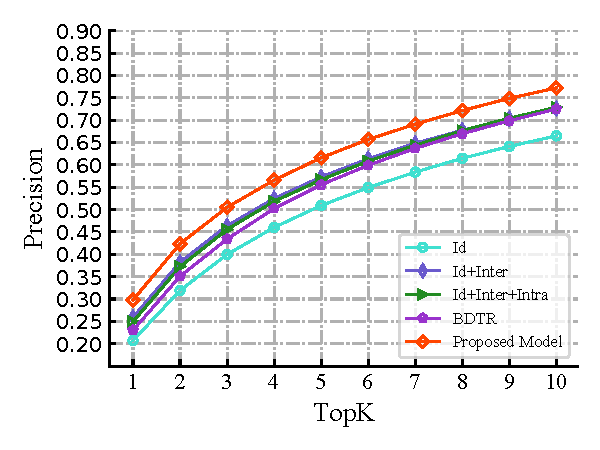
\includegraphics[height=5cm]{02/v_t_sysu_all.pdf}
    \caption{在SYSU-MM01 (All setting)下从visible模态到thermal模态的重识别结果}
  \end{subfigure}
  \hspace{1cm}
  \begin{subfigure}{0.45\textwidth}
    \centering
    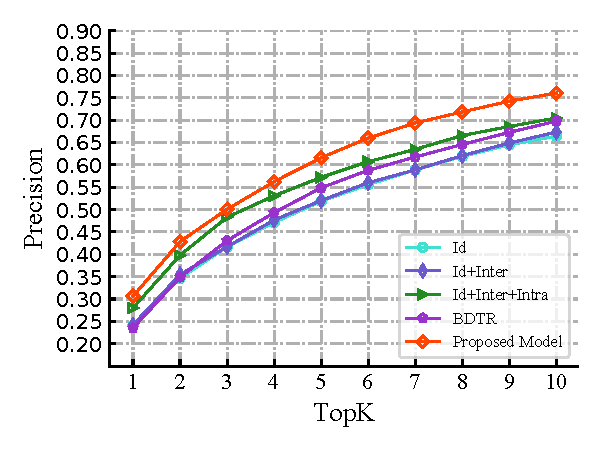
\includegraphics[height=5cm]{02/t_v_sysu_all.pdf}
    \caption{在SYSU-MM01 (All setting)下从thermal模态到visible模态的重识别结果}
  \end{subfigure}
  \begin{subfigure}{0.45\textwidth}
    \centering
    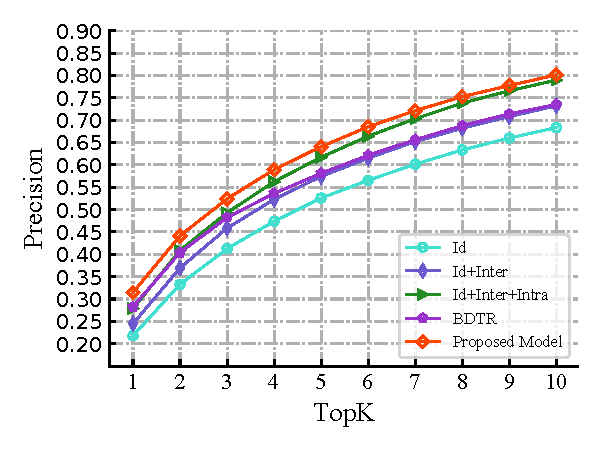
\includegraphics[height=5cm]{02/v_t_sysu_indoor.pdf}
    \caption{在SYSU-MM01 (Indoor setting)下从visible模态到thermal模态的重识别结果}
  \end{subfigure}
  \hspace{1cm}
  \begin{subfigure}{0.45\textwidth}
    \centering
    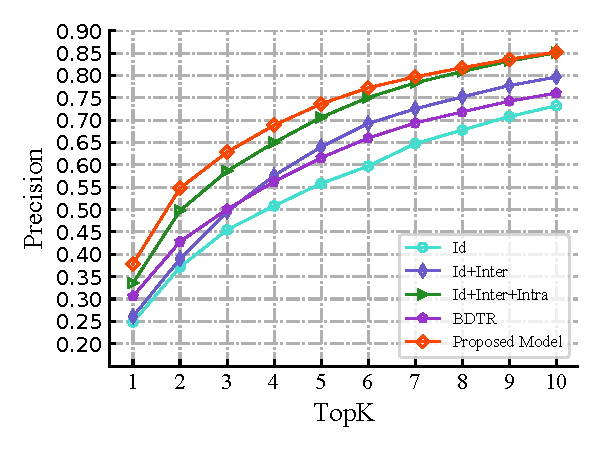
\includegraphics[height=5cm]{02/t_v_sysu_indoor.pdf}
    \caption{在SYSU-MM01 (Indoor setting)下从thermal模态到visible模态的重识别结果}
  \end{subfigure}
  \begin{subfigure}{0.45\textwidth}
    \centering
    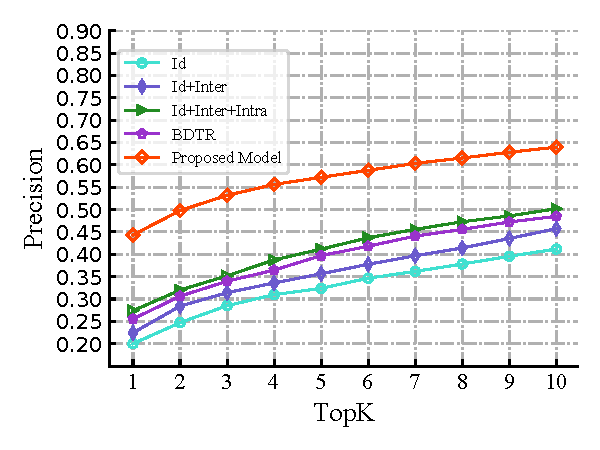
\includegraphics[height=5cm]{02/v_t_regdb.pdf}
    \caption{在RegDB下从visible模态到thermal模态的重识别结果}
  \end{subfigure}
  \hspace{1cm}
  \begin{subfigure}{0.45\textwidth}
    \centering
    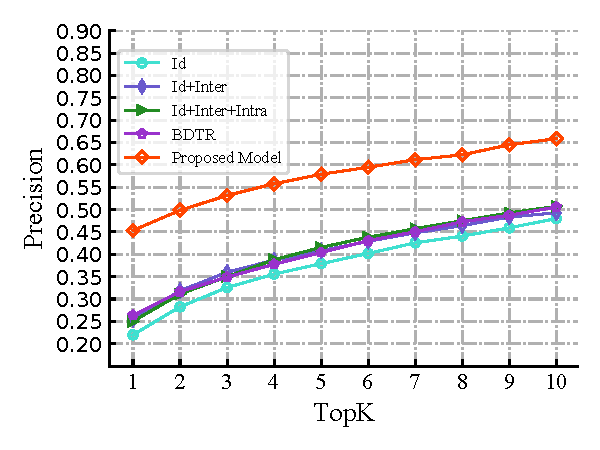
\includegraphics[height=5cm]{02/t_v_regdb.pdf}
    \caption{在RegDB下从thermal模态到visible模态的重识别结果}
  \end{subfigure}
  \bicaption[在两个不同数据集下的消融实验结果]{在两个数据集下模型的不同变种的行人重识别结果}{The person re-identification results of different variants on two public benchmark datasets.}
  \label{fig:ablation_res}
\end{figure}


\begin{enumerate}
  \item \textbf{Id}: 仅仅包含身份分类的损失函数$L_{Identity}$
  \item \textbf{Id + Inter}: 仅包含跨模态重识别损失函数$L_{Inter}$以及基于身份的分类损失函数$L_{Id} $的模型。
  \item \textbf{Id + Inter + Intra}: 不包含重建编码损失函数$L_{RE}$的模型。
  \item \textbf{BDTR}: 当时的基于双流神经网络的最先进模型。 由于我们的方法也是基于相同双流神经网络, 我们将BDTR也加入到消融实验进行对比研究。
  \item \textbf{Proposed Model}: 即本章提出的完整模型 \textbf{MAENet}
\end{enumerate}

由图~\ref{fig:ablation_res}可知, 仅包含分类损失函数的模型 \textbf{Id} 在~\textbf{SYSU-MM01} 和 \textbf{RegDB}上的所有测试场景均只能取得最低的性能。这是由于 \textbf{Id} 并不能有效的降低类内变化以及跨模态变化带来的影响。当加上 $L_{Inter}$损失函数后, 如图中的蓝色曲线所示, 模型在各个场景下都取得了性能上的提升。这是由于 $L_{Inter}$可以较大的对齐两个模态的特征, 降低跨模态差异带来的负面影响。同时当进一步加上$L_{Intra}$时, 如绿色曲线所示, 模型的性能进一步提升, 甚至可以显著的超越 \textbf{BDTR} 的性能。最终, 当我们加上本章提出的创新性的模态以及外表恒定的模块时候, 如红色曲线所示, 我们可以看到性能的显著提升。在 visible-to-thermal重识别场景, 这个模块在 \textbf{RegDB} 和 \textbf{SYSU-MM01} (all search)数据集上, 将$Rank1$准确率从$27.28 \%$, $24.93 \%$ 分别提升到了$44.32\%$ $32.33 \%$。在 thermal-to-visible的重识别场景中, 也可以观察到类似的性能提升。在 \textbf{RegDB}中$Rank1$ 准确度从 $25.00 \%$ 提升到了 $45.34 \%$ 而在 \textbf{SYSU-MM01} (indoor search) 从 $33.56 \%$ 提升到了 $37.86 \%$。这些显著的性能提升是由于我们提出的模态恒定以及外观恒定的网络以及损失函数可以帮助有效的对齐两个模态的特征, 降低模态间的差异, 降低跨模态变化以及模态内同一行人的不同变化带来的影响, 证实了这些不同的模块的有效性。

\section{总结}
本章针对图像检索的一个经典的应用行人重识别进行了深入的研究。本章针对行人重识别问题的一个非常具有挑战性的子问题-"跨模态行人重识别"进行了建模。 我们提出了一个崭新的神经网络框架以及对应的优化损失函数来进行学习。为了应对跨模态行人重识别的模态差异的带来的影响(Modality Discrepancy), 本章采取双流卷积神经网络分别将visible和thermal模态的照片映射到可比较的特征空间。同时, 基于autoencoder, 我们提出了一个模态和外表恒定的自编码网络架构 (modality and apperance invariant reconstructive embedding) 来提取出对于模态和外表都不变的特征。 为了进行重识别任务, 本章基于最大似然估计提出两种基于成对图片的重识别损失函数来进一步对齐两个模态的特征, 以及应对跨模态(Inter-modality Variation)和模态内的变化 (Intra-modality Variation)。
% !TEX root = ../main.tex
\chapter{基于深度哈希的大规模车辆重识别}
车辆重识别是现代智能交通系统中非常普遍的技术。在监控系统中, 车辆重识别可以用于对目标车辆进行自动化的监管, 定位, 以及在犯罪行为发生后进行的刑侦调查。传统的的重识别方法一般是通过将车辆照片映射到实值的特征向量并且通过欧式距离的计算将数据库中的照片根据距离进行排序来进行。然而, 尽管这样的方法可以取得较高的检索准确率, 这些高维的特征向量并不是为了快速索引匹配而设计的, 而且需要占用较大的内存空间, 同时欧式距离的计算也需要较大的计算量。 因此, 这样的方法并不适用于大规模的车辆重识别的场景中。 \par
为了解决这个难题, 本章提出了一个新型的车辆检索的框架 \textbf{DVHN}, 这是第一个将深度哈希学习引用到车辆重识别任务上的工作。 ~\textbf{DVHN}可以极大的降低内存开销并且提高检索的效率同时不会损失较多的准确度。具体来说, ~\textbf{DVHN} 通过联合的特征训练和哈希码生成训练, 使用深度卷积神经网络直接对每张图片学习一个紧凑的二进制编码。为了实现这一目的, 我们直接量化深度网络的输出, 生成离散的哈希编码, 并且增加限制条件使得哈希编码对于分类任务是最优的。 为了优化这个离散的哈希框架, 我们提出了一个交叉优化方法来同时优化离散哈希模块以及特征提取的深度神经网络。本章在两个标准的大规模车辆重识别数据集\textbf{VehicleID}和\textbf{VeRi}上进行了广泛的测试. 实验结果表明, 本章提出的算法\textbf{DVHN}在所有哈希长度上均远超当前最先进的方法。~\textbf{DVHN} 在哈希长度为 $2048$ 时可以在\textbf{VehicleID}(800)取得 $13.94 \%$ 和 $10.21 \%$的~\textbf{mAP} 和$Rank-1$ 精度提升。 在 \textbf{VeRi}数据集上, ~\textbf{DVHN} 可以在$Rank-1$上取得 $35.45 \%$的精度提升, 在~\textbf{mAP}上取得$32.72 \%$的性能提升。
\section{引言}
车辆重识别 (Vehicle Re-identification, Vehicle ReID)~\cite{liu2016deep, liu2017beyond, yan2017exploiting, guo2018learning, lou2019embedding, meng2020parsing} 由于其在智能交通系统, 智能安防领域, 以及在智能城市管理领域的广泛应用, 获得了计算机视觉研究人员的大量关注。\textbf{Vehicle-ReID}旨在给定一张查询的车辆照片, 在由不同监控摄像头拍摄的车辆照片组成的大规模车辆图片数据库中精确的找到属于同一辆车的其他照片。 一般的车辆重识别框架包含两个模块: ``特征学习模块'' 和 ``度量学习模块''。 (1)特征学习: 通过传统基于手工或者基于深度卷积神经网络的方法从车辆图片中提取有判别性的特征。 (2)度量学习: 使得上一步骤学习到的特征向量在低维空间可以保留原始图片的语义信息~\cite{chu2019vehicle}。也就是说, 语义不一致的图片在特征空间的距离尽量疏远, 而语义相近的图片应该尽量有接近的特征向量。 以往的车辆重识别方法已经在多种研究数据集上取得了令人瞩目的性能, 并且被工业界应用在一些现实任务中。 然而, 这些传统的车辆重识别方法并不能在现实生活中的大规模检索任务中进行应用。在大规模图像检索中, 被检索的图像中一般包含了数百万甚至上千万的图片数据。传统的车辆重识别方法一般有下面的劣势, 限制了其在大规模场景的应用。 首先, 在数据库中包含超大量的图片时候, 高维的实值特征向量的存储开销变得极其大。例如, 存储一个 $2048$维的浮点$64$类型的特征向量需要占据 $16$ 千字节(Kilobyte, KB)。对于一个数据库中具有1千万张图片的检索任务而言, 总共需要的内存高达 $150$ 吉字节 (Gigabyte, GB)。 除开内存开销, 检索时需要使用查询的特征向量与数据库中所有的存储的特征向量进行欧式距离的计算。然而, 欧式距离的计算耗时大~\cite{lin2015deep}, 也使得这种方法无法被应用在对检索速度要求较高的任务中。\par
近年来, 由于其低内存开销以及高检索效率, 深度哈希学习已经被广泛应用在通用的图片检索任务中。深度哈希的目标是通过学习一个哈希函数将图片映射到一个低维的汉明空间, 同时在汉明空间里保留其在原始图片的语义相似性~\cite{lin2015deep, cakir2019hashing, cao2016correlation, cao2017hashnet}。因为一个 $2048$位的汉明哈希码仅仅只需要占据 $256$ 字节的内存, 对于上面所述的1亿张图片的数据库只需要不到 $2.4$ GB的内存开销, 相比较基于实值的特征向量而言, 节省了 $147$ GB 的内存开销。另外, 如文章~\cite{ong2016improved}所述, 二进制汉明哈希码之间的汉明距离可以通过 CPU硬件指令 \textit{XOR} 进行加速。 通常来说, 汉明距离的计算可以实用几个机器指令来完成, 相比较欧式距离的计算来说, 极大的降低了计算的时间开销。 \par
被上述的深度哈希的优势所启发, 本章思考了将深度哈希算法直接引入到车辆重识别问题, 来完成大规模车辆重识别任务的可能性。尽管深度哈希在通用图片检索取得了较好的性能表现, 由于车辆重识别任务的独特性和难度, 直接应用这些深度哈希的算法并不能取得可以令人接受的性能表现。车辆重识别受光照变化, 背景繁杂, 遮挡, 以及不同拍照视角的影响导致了问题的困难性。传统的深度哈希方法很难学习到强健的有判别性的特征表示。例如, 一个经典的深度哈希方法~\textbf{SFH}~\cite{lai2015simultaneous} 是第一个端到端的监督的深度哈希框架。 它采用了一个三元损失函数并且使用一个divide-and-conquer模块来生成二进制哈希码。同时在深度卷积神经网络的输出后采取L1-norm来限制网络生成二进制的编码。然而, 这些方法是被设计用在当数据库中检索图片的类别较少的场景。 而在车辆重识别场景中, 数据库中有数以千计甚至上万的车辆, 而且每辆车包含的照片受上述多方面的影响具有较大的差异。 因此, 现成的深度哈希方法只能学习到此优的图像表征, 从而只能生成次优的二进制编码。\par
本章提出了一个新型的基于深度哈希的框架-\textbf{DVHN}-用于高效的的大规模车辆重识别场景。~\textbf{DVHN}充分的吸收了深度哈希的优点但是同时也没有牺牲检索的准确度。它主要包含四个部分: (1) 与以往基于图片对或者图片三元组的传统的哈希方法不同, 本章提出一种在每个批次输入中动态生成困难三元组的方法。(2) 一个基于深度卷积神经网络的特征提取方法。(3) 一个基于度量学习的哈希码生成模块来使得生成的哈希编码可以保留原始图片的视觉相似性。(4) 一个离散汉明哈希模块。 \par
对于保持相似性的度量学习方法, 我们采取一个基于困难三元组挖掘的三元损失函数 (batch-hard triplet loss)来尽量拉近视觉相似的图片在特征空间的距离, 相反, 推远视觉不相似的图片在特征空间的距离。另外, 为了使哈希码进来多保存具有判别性的行人特征, 本章另外加入了一个身份损失, 实际上是一个基于交叉熵的分类损失函数, 将每一个行人视作一个不同的类别。 对于离散汉明哈希模块, 我们直接使用不能导的 \textit{sign} 函数将神经网络的输出直接量化成离散的二进制编码, 并且限制这些学习到的二进制编码是对于分类最优的。 因为 \textit{sign} 函数不可导, 无法通过反向传播进行端到端的训练, 我们设计了一个新型的交叉优化方法来对~\textbf{DVHN}进行优化。在测试阶段, 对于所有查询图片以及数据库中的图片, 我们将它们编码成二进制的哈希码,然后将所有的数据库中的图片通过其与查询图片的哈希码的汉明距离进行从小到大的排序。 \par
本章主要做出如下的贡献:
\begin{enumerate}
    \item 本章分析了阻碍现有的车辆重识别的算法在大规模现实场景应用的主要障碍。我们进行了最初期的使用深度哈希学习来进行大规模车辆重识别的尝试。
    \item 本章提出了一个新型的框架, 以一种端到端的方式对车辆图片学习紧凑的哈希编码。本章提出一个新型的离散汉明哈希模块来学习二进制哈希编码, 同时保证哈希编码在分类任务上是最优解。为了解决困难的离散优化的问题, 我们采取一种交叉优化的方法, 通过离散编码学习到二进制哈希码后, 通过二进制哈希码以及度量学习的损失函数来监督训练神经网络进行表征学习。
    \item 本章基于Pytorch实现了多个先进的深度哈希算法, 并且仔细完备的训练并且测试了它们在标准的车辆重识别数据集上的性能。本章从头训练了72个模型, 对这一方向的研究提供了宝贵的基础数据。通过全面的测试以及比较, 我们证实了本章提出的\textbf{DVHN}算法的有效性, 并且证实了本章的相比较现有的先进算法可以获得极高的性能增长。
\end{enumerate}

\section{相关工作}
在这一小节, 我们主要阐述先前的与本章提出的算法相关的工作。我们主要根据它们是否采用了二进制特征向量来将它们分为两个类别: ``基于哈希的图像检索'' 和 ``车辆重识别''。
\subsection{基于哈希的内容检索}
近年来基于哈希的大规模内容检索已经获得了工业界和学术界的广泛关注~\cite{indyk1997locality, weiss2008spectral, gong2012iterative, heo2012spherical, jegou2010product, ge2013optimized, li2018deep}。根据它们提取特征的方法, 现有的哈希方法主要可以分为两个类别: 浅哈希方法和基于深度学习哈希方法。\par
典型的浅哈希方法通常是基于手工特征来学习哈希编码。一个经典的这方面的算法是局部敏感性哈希 LSH~\cite{indyk1997locality}, 其通过寻找一个局部敏感的哈希族来进行哈希编码的生成。这种哈希族内的哈希函数对于相似的对象生辰生成的哈希码会有碰撞的概率远大与不相似的对象。随后, 基于 LSH, Charikar等人提出 SIMHASH~\cite{charikar2002similarity} 通过结合取整方法实现一系列的保距哈希函数。尽管基于 LSH 的方法取得了不错的性能, 但是她们需要比较长的哈希编码才能取得较好的性能结果。 2008年, Weiss 等人~\cite{weiss2008spectral} 提出了通过最小化图像对的带权的汉明距离来生成哈希编码。尽管这些基于手工特征的哈希方法取得了一定程度上的成果, 但是当被应用到具有较大的类内变化(intra-class variation)的现实数据中时, 由于基于手工的特征提取方法无法精确的保存图片中具有判别力的部分, 这些方法只能取得较低的性能表现。\par
考虑到这一点, 基于深度学习的哈希方法开始涌现~\cite{cao2017hashnet, fan2020deep, li2015feature, zhu2016deep, liu2016deep}。根据这些方法是否会使用到人工标注的标签进行监督训练, 基于深度学习的哈希方法也可以分为: 监督的哈希方法和无监督的哈希方法。无监督的哈希方法通过探索数据内部自带的特征信息来生成二进制码。经典的例子有~\cite{song2018binary, yang2019distillhash, tu2020mls3rduh, qiu2021unsupervised, luo2020cimon}。具体来说, Song等人~\cite{song2018binary} 提出一个二进制的生成对抗网络来通过一种无监督的方式将图片嵌入成二进制码。具体来说, 通过Generator在encoder生成的二进制码上进行条件生成原图片, 通过Discriminator进行判别生成的原图片的优劣, 可以促使encode生成的二进制哈希码保存更多原始图片中的信息。Yang 等人提出了 DistillHash~\cite{yang2019distillhash}, 在原始数据集上生成一个提炼的新的包含很多数据对的数据集, 每个数据对被认为是来自同一个类别, 也就充当了监督训练的标签。 Tu 随后提出 MLS3RDUH~\cite{tu2020mls3rduh}  引入一个机制通过探索特征内在的流型结构来通过数据的余弦相似度重建局部的语义相似度。 Qiu ~\cite{qiu2021unsupervised}提出通过采用带有信息瓶颈的对比学习来进行无监督的哈希学习。随后, Luo 等人提出 Cimon~\cite{luo2020cimon}通过全局的优化以及相似性的统计分布来得到可靠并且光滑的指导。本章的工作属于带监督的哈希范畴, 通过人工标注的标签提供监督信号。2014年, Xia~\cite{xia2014supervised} 提出第一个基于深度学习的监督哈希框架。它提出一种两阶段哈希的方法先将相似度矩阵$S$ 分解成汉明矩阵$H$ 和 $H^T$的乘积, 其中 $H$的每一行代表一个训练图片数据的哈希编码。然后, 在下一阶段, 卷积神经网络通过第一阶段得到的哈希码作为监督信号来进行监督训练。随后, Lai等人提出一个端到端的深度哈希框架~\cite{lai2015simultaneous}, 通过三元损失函数以及一个divide-and-encode 模块来端到端的学习图像特征以及生成二进制的哈希编码。Zhu 随后提出 DHN~\cite{zhu2016deep} 基于贝叶斯学习框架设计一个基于成对训练数据的算是函数来进行相似度保留的哈希码生成。Cao 随后提出 DCH~\cite{cao2018deep} 通过使用一个柯西分布 (cauchy distribution) 来替换DHN框架中使用sigmoid函数来度量两张图片输出的相似概率。Wu 提出了一个增量哈希框架 (incremental hash)~\cite{wu2019deep}, 这个框架不需要每次当数据库中的图片数量增加的时候重新训练模型, 更加具有现实可用性。 Fan 随后提出 DPN~\cite{fan2020deep} 通过一个深度极化损失(polarized loss)来监督模型进行二进制哈希码的生成, 使得不再需要加入常用的量化损失函数来控制模型的输出和量化后的二进制码的误差。尽管相比较无监督的方法, 基于监督的深度哈希取得了更加优越的性能表现, 这些方法并不是为了大规模车辆重识别而设计, 没有考虑到车辆重识别任务具有的特殊的挑战, 在Vehicle ReID任务上只能取得一般的性能表现。 \par
\subsection{基于深度学习的车辆重识别}
由于车辆重识别在数字监控, 智能交通~\cite{zhang2011data}, 城市计算~\cite{zheng2014urban}等领域的大规模应用, 基于深度学习的车辆重识别在这些年开始受到工业界和学术界的大规模的关注~\cite{liu2016large, liu2016deep, wang2017orientation, liu2017provid, bai2020disentangled, meng2020parsing}。车辆重识别由于其较大的类内差异(Intra-class variation)和较小的类间差异(Inter-class variation)而非常具有挑战性, 这是由于不同的车由于其属于同一品牌或者统一模具生产而外观非常相似。一部分的工作聚焦在提高学习到的特征表示的辨别力上。 Liu~\cite{liu2017beyond} 提出一个双流的神经网络来将不同模态的车辆照片映射到可以比较的欧式空间。Yan~\cite{yan2017exploiting} 提出通过探索多粒度的排序限制来学习特征。随后, Guo 等人提出通过一种从粗粒度到细粒度的学习方法来学习更加强健的特征表示。2019年, He~\cite{he2019part} 采取了提取车辆的局部分块的表征来帮助全局的特征训练。Lou ~\cite{lou2019embedding}设计了一个端到端的就对抗学习的网络来学习有判别性的特征。
Zheng ~\cite{zheng2020vehiclenet} 提出了另一个大规模车辆重识别的数据集 \textbf{VehicleNet}并且设计了一个两阶段学习框架来进行检索训练。Jiang~\cite{jiang2021robust}提出通过一个基于分块学习以及将车辆的刚性结构先验信息加入神经网络来学习强健的特征表示。 2022年, Li~\cite{li2022super} 提出了一个基于超分的车辆模块协同网络 (SPCN)来进行车辆重识别。 \par
另一部分的车辆重识别工作主要关注学习对视角不变 (viewpoint invariant)的特征~\cite{wang2017orientation, zhou2018aware, tang2019pamtri, bai2020disentangled}。2017年, wang提出通过定义多个关键部位, 对关键的部位进行局部特征抽取而得到对朝向不变的特征表。同时提出一种在空间和时间维度上的标准化策略来提高检索的准确性。Zhou 随后提出一种新的机制~\cite{zhou2018aware}通过单个视角的信息生成多视角的特征。 Zhou 提出一种对于车辆摆放信息感知的多任务学习算法来学习对于视角不变的特征。Bai ~\cite{bai2020disentangled}随后提出可以将特征解耦成对于朝向特有的(oritentation-specific)以及朝向恒定的(orientation-invariant)的特征来进行重识别任务。Zhu ~\cite{zhu2019vehicle}提出基于四元组的损失函数来进行特征抽取以及度量学习而 Chen 等人~\cite{chen2020vehicle}则提出了一种端到端的基于距离的深度神经网络, 它可以学会区分车辆的局部和全局的不同性来进行重识别。Liu 提出一种车辆解析方法来学习有判别度的车辆局部信息以及建造了一个分块的邻接图来对每个不同部分的特征的关联进行建模。为了减轻剧烈的外表变化带来的影响, Jin 随后设计了一个新型的多中心度量学习的框架来对车辆外观的隐藏的观察点进行建模而不需要额外的监督标签。尽管这些方法取得了一些成果, 以上提及的车辆重识别方法都是基于实值的特征向量并且依赖于欧式距离的计算来对数据库中的图片进行排序和检索。这些方法无法适用于实际现实中的大规模车辆重识别的场景, 以及对与检索速度要求较高的场景。
\section{基于深度哈希的重识别算法}
\subsection{本章主要符号定义以及问题定义}
在本章中, 我们使用书法大写字母 (calligraphic uppercase), 例如 $\mathcal{F}$ 来表示映射函数。我们使用粗体大写字母 (Bold-face uppercase) 如 $\mathbf{B}$ 来代表集合. 粗体小写字母如 $\mathbf{b}$在全章中代表向量。我们使用斜大写字母 (Italic uppercase)来代表图片, 如 $\textit{I}$。 同时, 在全章中, sign激活函数直接由 $\textit{sign}$ 来表示。\par
\textbf{问题定义:} 假设 $\mathbf{X} = \{\textit{I}_i\}^N_{i=1}$ 是一个包含了$N$个训练数据的车辆检索训练数据集。 $\mathbf{Q} = \{I_i^q\}^{N_{q}}_{i=1}$ 和 $\mathbf{G} = \{I^g_i\}^{N_{g}}_{i=1}$是对应的查询集和被检索的数据库图片集。$\mathbf{Y} = \{\textit{y}_i\}^N_{i=1} \in \{0,1\}^C$是对应的标签集, 其中$C$是对应的车辆数。 基于深度哈希的车辆重识别的目标是学一个非线性的哈希函数 $\mathcal{H}: I \mapsto \mathbf{b} \in \{0,1\}^K $, 通过输入一张图片$\it{I}$并且将其映射成一个 K 位的二进制哈希向量 
$\mathbf{f}$。

同时需要保证每张车辆照片经过映射后的哈希向量需要保存原车辆照片的视觉相似性。整个基于学习的哈希函数可以由如下公式表示:
\begin{equation*}
    \mathbf{b}  = \mathcal{H}(I) = \mathbf{\it{sign}} (\mathcal{F}_{hash}(\textit{I})) 
\end{equation*}
其中 $\mathcal{F}_{hash}$ 代表生成哈希向量的非线性的深度神经网络, $\it{I}$是输入的车辆照片。 $\mathbf{\it{sign}(v)}$是一个符号函数, 它输出 $1$ 如果 $v \geq 0$, 反之输出$-1$。
本章提出一个新型的针对车辆重识别设计的哈希框架~\textbf{DVHN}。在接下来的小节中, 我们会着重详细的介绍模型的实现细节。我们先简单的介绍了我们的基础神经网络架构。随后, 我们介绍用于进行相似度学习的度量方法。之后, 我们详细的阐述了离散哈希学习的方法。接着, 我们介绍了采用的优化整个架构的交叉优化方法。最后, 我们简单的介绍了训练和测试的检索过程。
\begin{figure}[!htp]
    \centering
    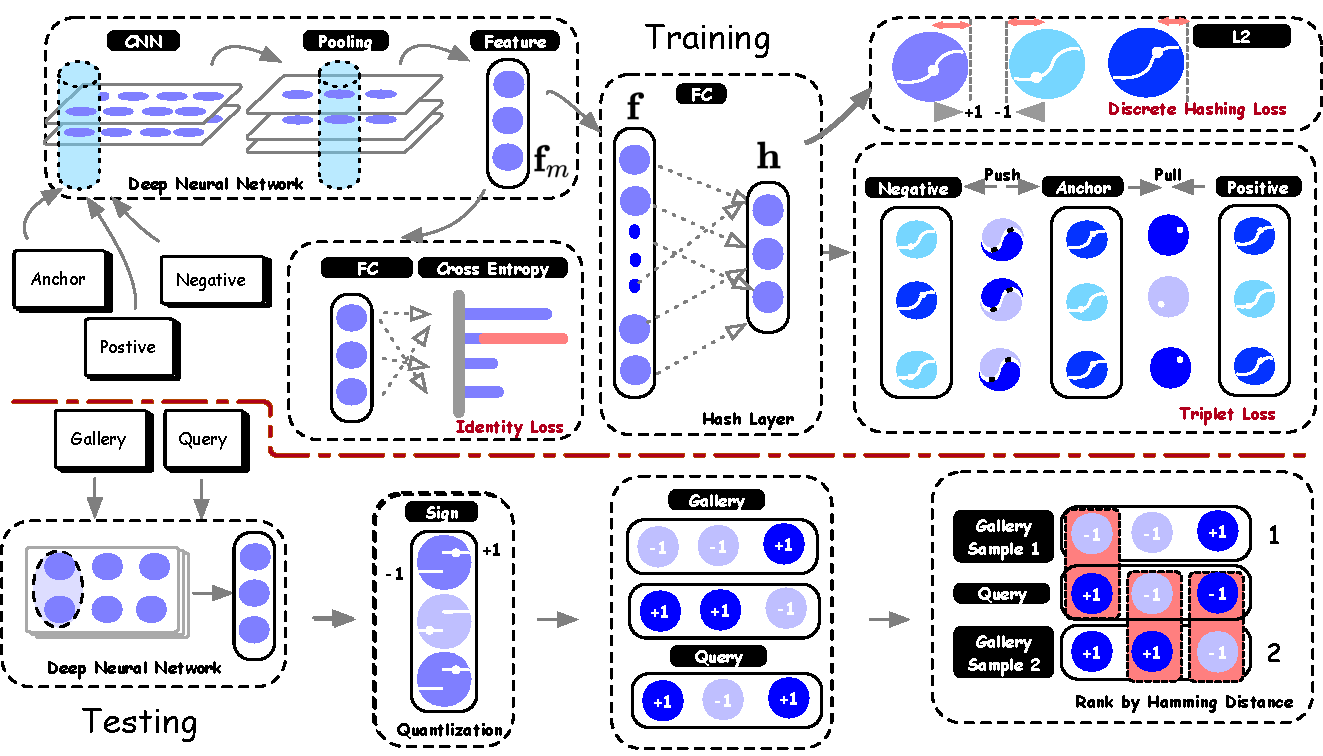
\includegraphics[width=15cm]{03/architecture.pdf} \\
    \bicaption[基于深度哈希的大规模车辆重识别框架]
      {基于深度哈希的大规模车辆重识别框架图,包含两个阶段。上图阐述神经网络学习生成有效的哈希编码的过程, 包含一个身份损失和一个基于困难组的三元损失函数以及离散哈希模块。下图阐述了测试过程。在测试阶段, 检索和数据库图片都被编码成二进制编码, 然后通过与检索的图片的汉明距离进行排序。}
      {The framework of DVHN. It basically contains two stages. The top part illustrates the process of learning to produce effective hash codes. The
      bottom demonstrates the testing process. During testing, the query and gallery images are encoded into binary discrete hash codes with the trained model.
      Then, the gallery images are ranked by computing their Hamming distances to the query image.}
   \label{fig:archvehicle}
\end{figure} 
\subsection{用于生成哈希向量的网络}
我们采取 \textbf{ResNet-50}~\cite{he2016deep} 作为基础的特征提取神经网络, 用$\mathcal{F}_{\theta}$表示。图片$\it{I}_i$丛$\mathcal{F}_{\theta}$输出的特征向量$\mathbf{f}_i$的过程如下所示:
\begin{equation}
    \mathbf{f}_i = \mathcal{F}_{\theta}(I_i)
\end{equation}
为了生成有不同长度的哈希码, 我们基于主干网络设计了一个额外的哈希层。具体来说, 在全局平均池化层(Global average pooling)后, 我们增加了一个全连接层, 它接收$M$维度的特征向量 $\mathbf{f}$ 输出 $K$维度的连续的哈希向量:
\begin{equation}
    \mathbf{h} = \mathcal{F}_{\theta_1}(\mathbf{f}) = \mathbf{f}W_1^T + \textbf{b}
\end{equation}
其中$W_1 \in \mathbb{R}^{M\times K}$ 和 $\mathbf{b} \in \mathbb{R}^{K}$ 代表全连接哈希层的权重以及偏差参数。 而$K$是代表汉明哈希码的长度。值得注意的是, 不像之前的深度哈希方法采取 \textit{tanh} 或者 \textit{sigmoid} 函数来将神经网络的输出强制接近二进制输出, 我们采取一个量化损失函数 $quantization loss$ 来使得神经网络的输出接近二值, 具体细节会在接下来的小节中详细阐述。
\subsection{基于相似度保留的特征学习}
我们将输入的车辆图片组织成三元样本, 并且将哈希函数学习的问题转化为一个相似度保留的特征学习问题。具体来说, 被Hermans~\cite{hermans2017defense}的工作所启发, 我们在每次输入前, 先随机采样 $P$ 个车辆, 随后, 我们随机对于每一辆车采样$K_1$张图片来组成一个具有$P*K_1$张图片的批次输入。对于在批次中的每一张图片$\it{I}_i$, 我们会将它视为锚定图片(anchor image), 然后找到一张和$\it{I}_i$属于同一辆车但是距离最远的图片$\it{I}_i^+$。同样的方法,我们也会在批次中找到一个在某个距离指标$D$下最难的负样本$\it{I}_i^-$, 即和图片$\it{I}_i$属于不同的一辆车但是距离却最近的图片。 通过这样的方法, 我们可以得到一个训练数据集 $\mathbf{T_{1}} = \{(I_i, I_i^+, I_i^-)\}_{i=1}^{P*K_1}$。对于每一张图片 $I$, 对应的连续的哈希向量 $\mathbf{h}$ 可以通过以下公式得到:
\begin{equation}
    \mathbf{h}_i = \mathcal{H}(I_i) = \mathcal{F}_{\theta_1}(\mathcal{F}_{\theta}(I_i))
\end{equation}
其中 $\mathbf{h}_i$是$\it{I}_i$对应的哈希向量。 $\mathcal{F}_{\theta}$代表主干非线性的卷积神经网络,而$\mathcal{F}_{theta_1}$则代表基于全连接神经网络的哈希层。因为我们的目标是需要保存图片在汉明空间的相似性, 我们提出了以下的限制:
\begin{equation}
    \mathcal{D}_H(\mathbf{h}_i, \mathbf{h}_i^+) < \mathcal{D}_H(\mathbf{h}_i, \mathbf{h}_i^-) 
\end{equation}
其中, $\mathcal{D}_H$代表了汉明距离。这个公式表明, 我们希望anchor图片和其最难的正样本$\it{I}_i^+$的汉明剧喽应该要小于和对应的最难负样本的距离。我们可以观察到汉明距离与内积有以下的线性关系:
\begin{equation*}
    \mathcal{D}_H(\mathbf{h}_i,\mathbf{h}_j) = \frac{1}{2}(B - \langle \mathbf{h}_i,\mathbf{h}_j \rangle)
\end{equation*}
因此, 在本文中我们使用内积来作为汉明距离的一个替代计算方法, 以便于汉明距离的计算。\par
接下来, 我们可以用公式表示基于三元图片组的相似性保留损失函数:
\begin{equation}
    \begin{array}{l}
    \begin{aligned}
    L_{Triplet} (h)
    &= \sum_{i \in \mathbf{T_{1}}} [\alpha + \mathcal{D}_{H}(\mathbf{h}_i,\mathbf{h}_i^+) - \mathcal{D}_{H}(\mathbf{h}_i, \mathbf{h}_i^-)]  \\
    &=  \sum _{i=1}^{P} \sum _{a=1}^{K}[\alpha+\overbrace{\max _{p=1 \ldots K}\left\|e_{i}^{a}-e_{i}^{(p)}\right\|_{2}}^{\text {hardest positive}}  \\
    &- 
    \underbrace{\min _{n=1 \ldots K \atop j=1 \ldots P} \|e_{i}^{a}-e_{j}^{(n)}\|_{2} }_\textrm{hardest negative}]
    \end{aligned}
    \end{array}
    \label{eq:tripletloss}
    \end{equation}
其中 $P$代表输入批次中有的车辆总数, $K$ 代表批次中每辆车包含的图片数量。$e_{i}^a$ 代表属于车辆 $i$ 的anchor的向量。$\alpha$代表三元损失函数的边界参数。\par
为了使学习到的特征向量可以保留更多的具有判别力的特征, 我们另外在主干网络输出的特征向量$\mathbf{f}$后增加来了一个身份损失函数(identity loss)。为了实现这个目标, 我们另外增加了一个全连接层充当分类器。如图~\ref{fig:archvehicle}所示, 一个输出维度的$N_C$的全连接层$\mathcal{F}_{\theta_2}$被添加在$\mathbf{f}$之后, 其中$N_C$是训练数据集中的车辆数。通过将每一辆车当成分类任务中的一个类别, 我们可以将身份损失函数表示成为一个分类损失函数:
 $L_{Identity}$ as:
\begin{equation}
L_{Identity}(f)=-\sum_{i=1}^{P*K} \log \frac{e^{{W}_{y_{i}}^{T} \mathbf{f}_i }}{\sum_{k_1=1}^{N_C} e^{{W}_{k_1}^{T} \mathbf{f}_{i}}}
\label{eq:identity}
\end{equation}
其中 $W_k$是对于第$k$辆车的权重向量, $P \times K_1$是批次中所有的图片, $N_C$是输入批次中总共的车辆数。
\subsection{离散哈希学习}
离散哈希模块核心假设是学习到的二进制汉明哈希码需要保存图片的类别信息。具体来说, 对于每一张图片$\it{I}_i$, 二进制汉明码$\mathbf{b}_i$可以通过对连续的哈希向量$\mathbf{h}_i$使用 \textit{sign} 函数得到:
\begin{equation}
    \mathbf{b}_i = \textit{sign}(h_i) = \textit{sign}(\mathcal{H}(\textit{I}_i))
\end{equation}
其中 $\textit{sign}(x)$的定义如下:
\begin{equation}
\operatorname{sgn}(x)=\left\{\begin{array}{c}
1, x>=0 \\
-1, x \le 0 
\end{array}\right.
\end{equation}
我们随后采取一个简单的线性分类器利用二进制的哈希码来重建真是的标签如下所示:
\begin{equation}
    y_i = W^T_h\mathbf{b}_i
\end{equation}
其中  $y_i \in \{0,1\}^C$, $C$是车辆的数量, $W_h$是分类器的权重参数。我们可以将离散哈希损失函数写作:
\begin{equation}
    L_{Quant}(\mathbf{b}) =  \mu\sum_{i=1}^{N}\left\|y_{i}-W^{T}_h \mathbf{b}_{i}\right\|_{2}^{2}+\nu \|W_h\|_{F}^{2}  
\end{equation}
其中 $\|\cdot\|_{2}$ 是一个向量的 $l_2$ 范数 而$\|\cdot\|_{F}$ 则是一个矩阵的弗罗贝尼乌斯范数 (Frobenius norm )。
\subsection{交叉优化算法}
我们可以将最终的损失函数写作为:
\begin{equation}
    L_{Total} = \lambda L_{Triplet}(\mathbf{h})  + \sigma L_{Identity}(\mathbf{f}) + L_{Quant}(\mathbf{b})
    \label{eq:totall}
\end{equation}
其中 $\lambda$, $\beta$ and $\sigma$为三个预先定义的系数来控制各个部分的损失函数对目标函数的影响。最直接的优化这个目标函数的想法就是直接利用标准的随机梯度下降算法来优化这个目标函数~\ref{eq:totall}。然而, \textit{sign} 函数是不可导的, 梯度无法通过这个函数进行反向传播。因此, 目标函数的第三个部分$L_{Quant}$不能像第一第二个部分的损失函数一样用随机梯度下降算法直接优化。我们将第三个部分展开为:
\begin{equation}
    \begin{aligned}
     L_{Total} &= \lambda L_{Triplet}(\mathbf{h})  + \sigma L_{Identity}(\mathbf{f})) \\
     &+\mu \sum_{i=1}^{N}\left\|y_{i}-W_h^{T} b_{i}\right\|_{2}^{2}+\nu\|W_h\|_{F}^{2} 
    \end{aligned}
       \label{eq:totalfold}
   \end{equation}
为了绕过\textit{sign}函数到来的梯度消失的问题, 之前的工作一般采取\textit{tanh}和\textit{sigmoid}函数在训练阶段来生成接近二值的连续性的输出而在测试阶段再使用\textit{sign}函数来获得二值的哈希码。然而这样的优化方法是在优化原始目标的一个放松后的目标函数, 导致优化结果会偏离原始目标从而导致次优的哈希码~\cite{liu2016deep}。\par
考虑到这一点, 我们采取一种新型的交替优化方法 (alternative optimization) 模式在优化网络的时候保留哈希码的离散特性。与Li~\cite{li2017deep}和 Wang~\cite{wang2017deep}的工作相似, 我们引入了一个额外的变量将之前的优化公式~\ref{eq:totalfold}改写为: 
\begin{equation}
    \begin{aligned}
L_{Total} &= L_{Triplet}(h) + L_{Identity}(f) \\
&+\mu \sum_{i=1}^{N}\left\|y_{i}-W_h^{T} b_{i}\right\|_{2}^{2}+\nu\|W_h\|_{F}^{2} \\
&\text { s.t. } \quad \mathbf{b}_{i}=\operatorname{sgn}\left(h_{i}\right), \quad \mathbf{h}_{i} \in \mathbb{R}^{K \times 1}, \quad(i=1, \ldots, N)
\end{aligned}
\label{eq:var}
\end{equation}
其中 $\mathbf{h} = \mathcal{F}_{hash}(f) $是连续性的实值哈希向量, $\mathbf{f}$是主干深度卷积神经网络的特征输出。而 $\mathbf{b}$则是二值化的汉明哈希码。上述公式~\ref{eq:var}是一个受限制的优化问题, 可以用拉格朗日乘子法(Lagrange Multiplier Method)进行优化:
\begin{equation}
    \begin{aligned}
L_{Total} &= L_{Triplet}(h) + L_{Identity}(f) \\
&+\mu \sum_{i=1}^{N}\left\|y_{i}-W^{T}_h b_{i}\right\|_{2}^{2}+\nu\|W_h\|_{F}^{2} \\ 
     &+ \eta \sum_{i=1}^{N}\left\|\mathbf{b}_{i}-\operatorname{sgn}\left(\mathbf{h}_{i}\right)\right\|_{2}^{2} \\
&\text { s.t. } \quad \mathbf{b}_{i} \in \{-1,1\}^K, \quad \mathbf{h}_{i} \in \mathbb{R}^{K \times 1}, \quad(i=1, \ldots, N)
\end{aligned}
\label{eq:lagrange}
\end{equation}
在公式~\ref{eq:lagrange}中的最后一个部分可以被视作一个限制条件, 度量连续的哈希向量和离散的汉明哈希码之间的量化误差。受Li~\cite{li2017deep}等的公布所启发, 我们将公式~\ref{eq:lagrange}解耦合成两个子优化问题, 并且用一种交替优化等方法来解决。 \par
首先, 我们固定参数$b$和$W$, 优化目标可以被转变为:
\begin{equation}
    \begin{aligned}
        L &= \lambda L_{Triplet}(\mathbf{h}) + \sigma L_{Identity}(\mathbf{f}) \\
        &+ \eta \sum_{i=1}^{N}\left\|\mathbf{b}_{i}-\mathbf{h}_{i}\right\|_{2}^{2}
    \end{aligned}
    \label{eq:sgd}
    \end{equation} \par
其次, 主干网络的参数 $\theta$, 哈希全连接网络的参数 $\theta_1$ 和分类器的网络参数 $\theta_2$ 可以通过随机梯度下降和反向传播来进行优化。\par
接着, 我们固定  $\theta$, $\theta_1$, $\theta_2$ 和 $\mathbf{b}_i$, 问题被转换成了以下:
\begin{equation}
    L = \mu \sum_{i=1}^{N}\left\|y_{i}-W_h^{T} b_{i}\right\|_{2}^{2}+\nu\|W_h\|_{F}^{2} \\ 
    \label{eq:least}
\end{equation}
非常明显可以看到公式~\ref{eq:least}是一个最小二乘问题(Least squares problem)并且有一个相近形式的解法:
\begin{equation}
    W_h=\left(B B^{T}+\frac{\nu}{\mu} I\right)^{-1} B^{T} Y
    \label{eq:least1}
\end{equation}
其中 $B = \{\mathbf{b}_i\}_{i=1}^N \in\{-1,1\}^{K \times N}$ 并且 $Y = \{y_i\}^N_{i=1} \in \mathbb{R}^{C \times N}$。\par

最后, 在获得$W_h$的解后, 我们固定参数 $\theta$, $\theta_1$, $\theta_2$ 和 $W_h$ 从而得到以下的目标函数: 
\begin{equation}
    \begin{aligned}
&L=\mu \sum_{i=1}^{N}\left\|y_{i}-W_h^{T} \mathbf{b}_{i}\right\|_{2}^{2}+\eta \sum_{i=1}^{N}\left\|\mathbf{b}_{i}-\mathbf{h}_{i}\right\|_{2}^{2} \\
&\text { s.t. } \quad \mathbf{b}_{i} \in\{-1,1\}^{K},(i=1, \ldots, N)
\end{aligned}
\end{equation} 
我们采取离散循环坐标下降 (cyclic coordinate descent)方法来迭代式的一行一行的求解$B$, 如下所示:
\begin{equation}
    \min _{B}\left\|W_h^{T} B\right\|^{2}-2 \operatorname{Tr}(P), \quad \text { s.t. } B \in\{-1,1\}^{K \times N}
    \label{eq:binary}
\end{equation}
其中 $P=W_h Y+\frac{\eta}{\mu} H$。
\begin{algorithm}
    \caption{\textbf{DVHN优化算法}\label{algo:maindvhn}}
    \KwData{训练图片集 $\mathbf{I}$,~监督标签 $\mathbf{Y}$, ~学习率 $\epsilon$ and 损失函数系数 $\alpha$, $\beta$, $\sigma$~ 最大迭代轮数$T$}
    \KwResult{优化的网络结构参数 $\theta$,~$\theta_1$, $\theta_2$,~$W_h$ 和二进制的汉明哈希码$\mathbf{B}$;}
    $t \leftarrow 0$\;
    $\theta \leftarrow $ ImageNet预训练参数 \; 
    $\theta_1 \leftarrow $ ImageNet预训练参数 \; 
    $\theta_2 \leftarrow \textbf{Xavier}(\theta_{RV})$  \; 
    $W_h \leftarrow \textbf{Xavier}(W_h)$  \;
    $B \leftarrow \textbf{Xavier}(B)$  \; 
    \While{未收敛 \textbf{and} $t < T$}
    {
      $t \leftarrow t +1 $\;
      \For{$i\gets0$ \KwTo $100$ }{
        冻结参数 $W_h$ 和$\mathbf{B} $  \;
        采样$P$辆车, 对于每辆车$p \in P$采样 $K$张图片, \;
        得到一个批次数据集 $\mathbf{Y} = \{y_i\}_{i=1}^{p*K}$ \;
        $f_i = \mathcal{F}_\theta(I_i)$   \;
        $h_i = \mathcal{F}_{\theta_1}(f_i)$  \;
        通过公式~\ref{eq:identity}计算 $L_{Identity}$ \;
        构建三元数据组 $\left\{ \mathbf{h}_i, \mathbf{h}_i^+,\mathbf{h}_i^-  \right\}$ \;
        通过公式~\ref{eq:tripletloss}计算 $L_{Triplet}$ \;
        通过\textbf{SGD} 来得到梯度$\nabla_{\theta_*}$~$*\in \{\theta,\theta_1,\theta_2\}$ \;
        $ \theta_* \leftarrow \alpha ( \theta_* - \nabla_{\theta_*}) $ \;
      }
      冻结参数$\theta,~\theta_1,~\theta_2$, 通过公式~\ref{eq:least}更新 $W_h$ \;
      冻结参数$\theta,~\theta_1,~\theta_2,~W_h$, 通过公式~\ref{eq:binary}更新 $\mathbf{B}$ \;
    }
    \end{algorithm}
\subsection{全局的训练算法}
总共的\textbf{DVHN}的训练优化算法如算法~\ref{algo:maindvhn}。我们有一个训练数据集$\mathbf{T}$和对应的标签集 $\mathbf{Y}$。最初的学习速率被设置成 $\epsilon$, 并且设置好三个在公式~\ref{eq:totall}控制各个部分影响的三个系数 $\alpha$, $\beta$, $\sigma$ 和边界参数 $\alpha$。 总共的训练迭代次数设置为 $T$。 \par
我们首先用在\textbf{ImageNet}预训练好的resnet-50参数来初始化$\theta$。对于哈希层和分类器的参数$\theta_1$和 $\theta_2$, 我们使用随机初始化的方法, 对于最初的计数器$t$, 我们设置为$0$。 \par
当模型还没有收敛并且迭代次数$t$ 小于总共的迭代次数$T$时, 我们进行如下的操作: 首先我们将迭代的计数器$t$增加$1$, 然后将下面操作进行$100$次:
\begin{enumerate}
    \item 首先, 我们冻结离散哈希模块的参数$W_h$ 和二进制哈希码$\mathbf{B}$。
    \item 随后, 我们构建一个批次的训练数据 $\mathbf{I}_b$, 其一共包含 $P \times K$张图片。$P$ 是所有的车辆数, $K$是随机对于某辆车抽样的照片数量。 对应的标签集$\mathbf{Y}_b$也同样建立。
    \item 随后, 通过随机梯度下降和反向传播更新得到对于$\theta, \theta_1$ 和 $\theta_2$的梯度$\theta_*$。
    \item 随后, 通过学习率$\alpha$来更新网络参数。
\end{enumerate}
在经过100次上述操作后, 我们冻结$\theta, \theta_1, \theta_2$, 并且通过公式~\ref{eq:least}来更新$W_h$。随后, 我们冻结 $\theta, \theta_1, \theta_2, W_h$, 并且通过公式~\ref{eq:binary}来逐行更新$\mathbf{B}$。

\subsection{检索过程}
在这一小节, 我们阐述如何在给定一个训练好的模型下进行高效的车辆重识别。通常, 给定一个查询数据集$\mathbf{Q}$和被检索的数据集$\mathbf{G}$。对于每一张查询图片$q_k$,任务是检索出在$\mathbf{G}$中和$q_k$属于同一辆车的图片。在测试阶段, 我们通过下面式子得到其离散二进制哈希码:
\begin{equation}
    \mathbf{b}_k^q = \mathbf{\it{sign}(\mathcal{F}_{\theta_1}(\mathcal{F}_{\theta}(\it{I}^q_k)))}
\end{equation}
随后, 用同样的方式对于所有在$\mathbf{G}$中的图片 $\mathbf{G} = \{\it{I}^g_k\}_{k=1}^{N_g} $, 我们得到一个二进制哈希码集合  $\mathbf{H^g} = \{\mathbf{b}_k^g\}_{k=1}^{N_g}$。随后, 我们可以通过被查询的二进制哈希码和检索的哈希码之间的汉明距离来进行对数据库中照片的排序。 我们注意到汉明距离$\mathcal{D}_H$和内积 $\langle\cdot, \cdot \rangle$有一个线性关系,如下所示:
\begin{equation}
    \mathcal{D}_H(\mathbf{b}_i,\mathbf{b}_j) = \frac{1}{2}(K - \langle \mathbf{b}_i, \mathbf{b}_j \rangle)
\end{equation}
其中$K$是二进制哈希码$\mathbf{b}$的长度。随后, 我们计算$\mathbf{b}_k^q$和所有被查询的数据库的哈希码$\mathbf{H}^g$的汉明距离。之后, 我们根据距离进行从小到大的排序。最后, 我们通过排序的汉明距离可以将$\mathbf{G}$中的图片进行对应的排序。

\section{实验结果与分析}
在这个章节, 我们仔细的评估测试了\textbf{DVHN}在标准的车辆重识别数据集上的性能, 并且与先进的其他算法进行了细致的对比。我们首先给出简要的介绍和我们模型的实现细节,数据集的具体信息以及评估指标。随后, 我们展示了详细的实验结果分析以及对比。
\begin{table}[!htpb]
    %% \centering % not needed
    \bicaption{各个先进深度哈希算法在车辆重识别数据集\textbf{VehicleID(800)}上的测试结果}{Vehicle Re-identification results of state-of-the-art deep hashing methods on \textbf{VehicleID (800)}}
    \centering
    \begin{tabular}{cccccc}
       \\ \hline
    \multicolumn{2}{l|}{Methods} & 256-bit & 512-bit & 1024-bit & 2048-bit   \\\hline
    \multicolumn{2}{l|}{SH~\cite{weiss2008spectral} (NeurIPS)} & 23.98 & 23.64 & 21.09 & 17.71  \\  
    \multicolumn{2}{l|}{ITQ~\cite{gong2012iterative} (TPAMI)} & 23.84 & 25.39 & 25.93 & 26.26  \\  
    \hline
    \hline
    \multicolumn{2}{l|}{DSH~\cite{liu2016deep} (CVPR)} & 30.56 & 32.53 & 34.22 & 33.62  \\
    \multicolumn{2}{l|}{DHN~\cite{zhu2016deep} (AAAI)} & 43.57 & 45.42 & 46.70 & 46.39  \\
    \multicolumn{2}{l|}{HashNet~\cite{cao2017hashnet} (ICCV)} & 62.95 & 64.52 & 65.96 & 66.61  \\
    \multicolumn{2}{l|}{DCH~\cite{cao2018deep} (CVPR)} & 37.08 & 34.55 & 26.04 & 24.13  \\
    \multicolumn{2}{l|}{DPN~\cite{fan2020deep} (IJCAI)} & 57.16 & 61.92 & 63.55 & 64.65  \\
    \hline
    \hline
     \multicolumn{2}{l|}{\textcolor{red}{DVHN} (ResNet50) }&\textcolor{red}{\textbf{71.61}} & \textcolor{red}{\textbf{73.69}} & \textcolor{red}{\textbf{75.86}} & \textcolor{red}{\textbf{76.82}} \\
     \hline
     \hline
    \end{tabular}
    \label{table:vid800}
  \end{table}
  \begin{table}[!htpb]
    %% \centering % not needed
    \bicaption{各个先进深度哈希算法在车辆重识别数据集\textbf{VeRi}上的测试结果}{Vehicle Re-identification results of state-of-the-art deep hashing methods on \textbf{VeRi}}
    \centering
    \begin{tabular}{cccccc}
       \\ \hline
    \multicolumn{2}{l|}{Methods} & 256-bit & 512-bit & 1024-bit & 2048-bit   \\\hline
    \multicolumn{2}{l|}{SH~\cite{weiss2008spectral} (NeurIPS)} & 3.33 & 2.75  & 2.08 &  1.57 \\  
    \multicolumn{2}{l|}{ITQ~\cite{gong2012iterative} (TPAMI)} & 4.80 & 4.95 & 5.04 & 5.14 \\  
    \hline
    \hline
    \multicolumn{2}{l|}{DSH~\cite{liu2016deep} (CVPR)} & 8.93 & 9.77 & 10.24 &  10.47 \\
    \multicolumn{2}{l|}{DHN~\cite{zhu2016deep} (AAAI)} & 13.85 & 13.93 & 14.31 & 13.71 \\
    \multicolumn{2}{l|}{HashNet~\cite{cao2017hashnet} (ICCV)} & 27.13 & 28.40 & 29.94 & 29.30  \\
    \multicolumn{2}{l|}{DCH~\cite{cao2018deep} (CVPR)} & 19.75 & 19.23 & 12.15 & 14.96  \\
    \multicolumn{2}{l|}{DPN~\cite{fan2020deep} (IJCAI)} & 10.03 & 11.26 & 13.52 & 13.58  \\
    \hline
    \hline
     \multicolumn{2}{l|}{\textcolor{red}{DVHN} (ResNet50) }&\textcolor{red}{\textbf{54.61}} & \textcolor{red}{\textbf{58.38}} & \textcolor{red}{\textbf{59.27}} & \textcolor{red}{\textbf{62.02}} \\
     \hline
     \hline
    \end{tabular}
    \label{table:veri}
  \end{table}

  \begin{table}[!htpb]
    %% \centering % not needed
    \bicaption{各个先进深度哈希算法在车辆重识别数据集\textbf{VehicleID (1600)}上的测试结果}{Vehicle Re-identification results of state-of-the-art deep hashing methods on \textbf{VehicleID (1600)}}
    \centering
    \begin{tabular}{cccccc}
       \\ \hline
    \multicolumn{2}{l|}{Methods} & 256-bit & 512-bit & 1024-bit & 2048-bit   \\\hline
    \multicolumn{2}{l|}{SH~\cite{weiss2008spectral} (NeurIPS)} & 19.96 & 20.06  & 16.32 &  13.83 \\  
    \multicolumn{2}{l|}{ITQ~\cite{gong2012iterative} (TPAMI)} & 20.23 & 21.45 & 21.27 & 22.23 \\  
    \hline
    \hline
    \multicolumn{2}{l|}{DSH~\cite{liu2016deep} (CVPR)} & 26.25 & 29.39 & 30.36 &  30.97\\
    \multicolumn{2}{l|}{DHN~\cite{zhu2016deep} (AAAI)} & 39.97 & 41.77 & 43.34 & 43.72 \\
    \multicolumn{2}{l|}{HashNet~\cite{cao2017hashnet} (ICCV)} & 56.89 & 69.99 & 60.05 & 60.88  \\
    \multicolumn{2}{l|}{DCH~\cite{cao2018deep} (CVPR)} & 27.23 & 25.33 & 19.67 & 18.45  \\
    \multicolumn{2}{l|}{DPN~\cite{fan2020deep} (IJCAI)} & 53.68 & 58.03 & 60.23 & 61.42  \\
    \hline
    \hline
     \multicolumn{2}{l|}{\textcolor{red}{DVHN} (ResNet50) }&\textcolor{red}{\textbf{66.67}} & \textcolor{red}{\textbf{69.12}} & \textcolor{red}{\textbf{71.83}} & \textcolor{red}{\textbf{72.72}} \\
     \hline
     \hline
    \end{tabular}
    \label{table:vid1600}
  \end{table}
  \subsection{模型的实现细节}
  本章的模型基于Pytorch~\cite{paszke2019pytorch}实现。详细的架构如图~\ref{fig:archvehicle}所示。具体来说, 在标准的\textbf{Resnet-50}的$f_{avg}$层后, 我们增加了一个输出为$K$维的全连接层, $K$代表哈希码的长度。对于分类器, 我们增加了一个输出为$N_C$维的全连接层, $N_C$代表类别的总数。这两个全连接层通过高斯随机初始化, 平均值为$0$, 标准哈为$0.01$。在训练过程中, 车辆总数$P$设置为$16$, 每辆车的照片数设置为$6$, 得到每一个批次的输入图片总数为$96$。 同时, 网络使用\textit{amsgrad}优化器进行优化。最初的学习速率$\epsilon$设置为$3e-4$, 权重衰减系数设置为$5e-4$, $\beta_1$设置为$0.9$而$\beta_2$设置为$0.99$。边界参数$\alpha$设置为$0.3$。对于控制各个损失函数在全局损失函数中的比重的系数 ($\lambda, \beta, \sigma$), 我们设置为$1$。

  \subsection{数据集}
  本节的实验采取了两个标准的车辆重识别任务中数据集进行训练与测试。为了实现与现有的先进方法比较的公平公正, 我们采取标准的训练集和测试集的划分方法来进行对比实验。两个数据集的具体信息如下:
  \begin{enumerate}
    \item \textbf{VehicleID}~\cite{liu2016deep}是一个大规模的车辆重识别数据集。它总共包含了$221,763$张来自$26,267$辆车的照片。在所有的照片中, $110,178$张来自$13,134$辆车的照片被选作为训练数据集。在测试中, 三个包含$800$, $1600$, $2400$辆车的子集从测试数据集中抽取出来, 组成 \textbf{VehicleID (800)}, \textbf{VehicleID (1600)}和 \textbf{VehicleID (2400)}三种模式。在本章中, 我们在\textbf{VehicleID (1600)}进行测试。对于\textbf{VehicleID (800)}, 查询数据集中包含$5,693$张来自$800$辆车的照片, 被检索的数据库中包含$800$张来自$800$辆车的照片。 对于\textbf{VehicleID (1600)}场景, 查询数据集包含$11,777$张来自$1600$辆车的照片而被检索数据库中包括了$1,600$张来自$1,600$辆车的照片。
    \item \textbf{VeRi}~\cite{liu2016deep}是一个现实世界都市监控车辆数据集。它包含了$50,000$张来自$776$辆车的图片。其中, $37,781$张来自$576$辆车的照片被当作训练数据集。在测试中, $1,678$张来自$200$辆车的照片被当作查询集, 剩余的$11,579$张照片当成被查询的数据库。
  \end{enumerate}
  \subsection{评价指标}
  我们采取平均准确率均值 (Mean Average precision, mAP) 以及累积匹配曲线 (Cumulative Matching Characteristic, CMC) 来评估方法的性能。\textbf{CMC}计算查询图片出现在检索返回列表不同位置的概率。由于它仅仅考虑第一次的匹配,使得其不适用于数据库中包含不止一张与查询图片属于同一辆车的图片的场景。因此我们加入\textbf{mAP}作为评估指标。~\textbf{mAP}同时考虑返回的查询结果的\textit{precison}和\textit{recall}其中 \textbf{mAP}的计算如下
  \begin{equation}
     \textbf{mAP} = \frac{1}{n} \sum_{k=1}^{k= N} \textbf{AP}_k
  \end{equation}
  其中$N$是查询的图片总数。由此式可知, $mAP$则为每张图片的平均准确率的平均值。其中~\textbf{AP}是计算precision-recall曲线下的面积, 如下所示:
  \begin{equation}
    \text { AP }^{=} \sum_{k=1}^{N} precision _{i}\left( recall _{k}- recall _{k-1}\right)
\end{equation}
其中 $k \in \{1, 2, 3, ..., N\}$并且$N$是被查询的数据集中照片的总数。

\subsection{与先进方法的对比结果}
在这一小节, 我们将~\textbf{DVHN}与先进的哈希算法在标准车辆重识别数据集上进行比较。具体而言, 用来比较的算法可以被划分为下面两个类别: ``无监督的哈希算法''和``有监督的深度哈希算法''。对于无监督的哈希算法, 我们包含了\textbf{SH}~\cite{weiss2008spectral}和\textbf{ITQ}~\cite{gong2012iterative}。值得注意的是, 这两种方法需要依赖特征提取器先从车辆照片提取特征向量。通常的做法是利用预训练好的深度卷积神经网络来提取特征。在本章中, 我们使用在imagenet上预训练后的\textit{AlexNet}来进行特征提取。对于监督学习的场景, 我们随后加入了~\textbf{DSH}~\cite{liu2016deep}, 第一批使用深度卷积神经网络来学习离散二进制哈希编码的工作。
\begin{figure}[!htp]
    \centering
    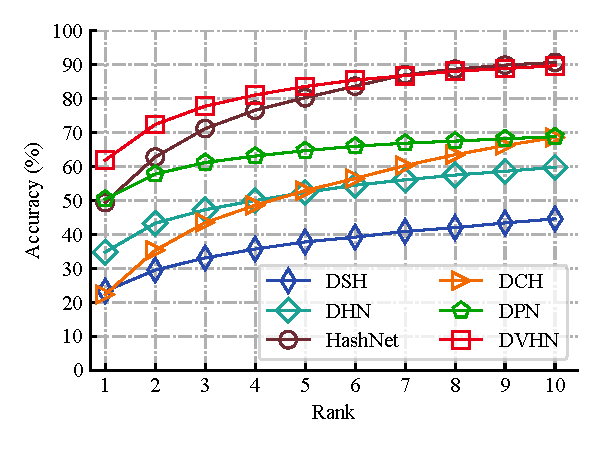
\includegraphics[width=13cm]{03/vid_256.pdf} \\
    \bicaption[在\textbf{VehicleID (800)}上256位的哈希算法的CMC结果]
      {256位哈希算法在\textbf{VehicleID (800)}上的结果}
      {CMC Results on \textbf{VehicleID (800)} of 256 bits}
   \label{fig:vid256}
\end{figure}

\begin{figure}[!htp]
    \centering
    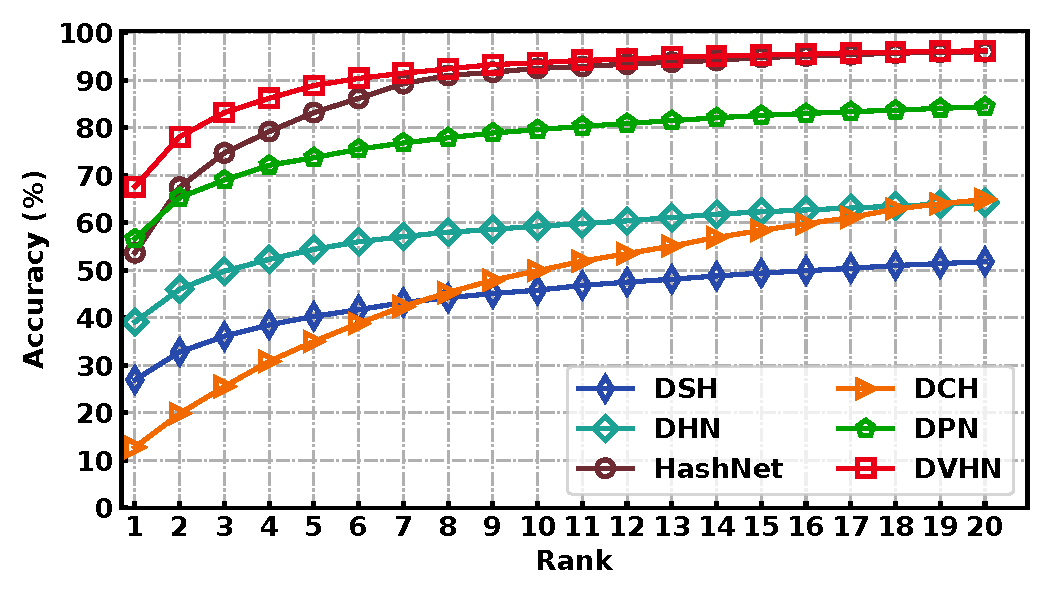
\includegraphics[width=13cm]{03/vid_2048.pdf} \\
    \bicaption[在\textbf{VehicleID (800)}上2048位的哈希算法的CMC结果]
    {2048位哈希算法在\textbf{VehicleID (800)}上的结果}
    {CMC Results on \textbf{VehicleID (800)} of 2048 bits}
   \label{fig:vid2048}
  \end{figure}

  \begin{figure}[!htp]
    \centering
    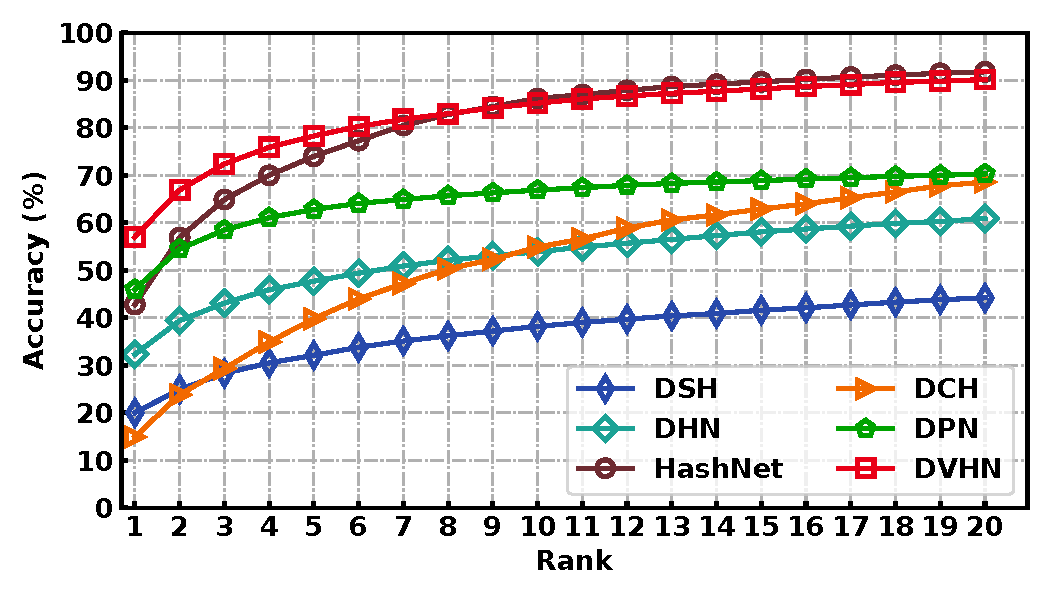
\includegraphics[width=13cm]{03/vid_1600_256.pdf} \\
    \bicaption[在\textbf{VehicleID (1600)}上256位的哈希算法的CMC结果]
    {256位哈希算法在\textbf{VehicleID (1600)}上的结果}
    {CMC Results on \textbf{VehicleID (1600)} of 256 bits}
   \label{fig:vid1600_256}
  \end{figure}
  \begin{figure}[!htp]
    \centering
    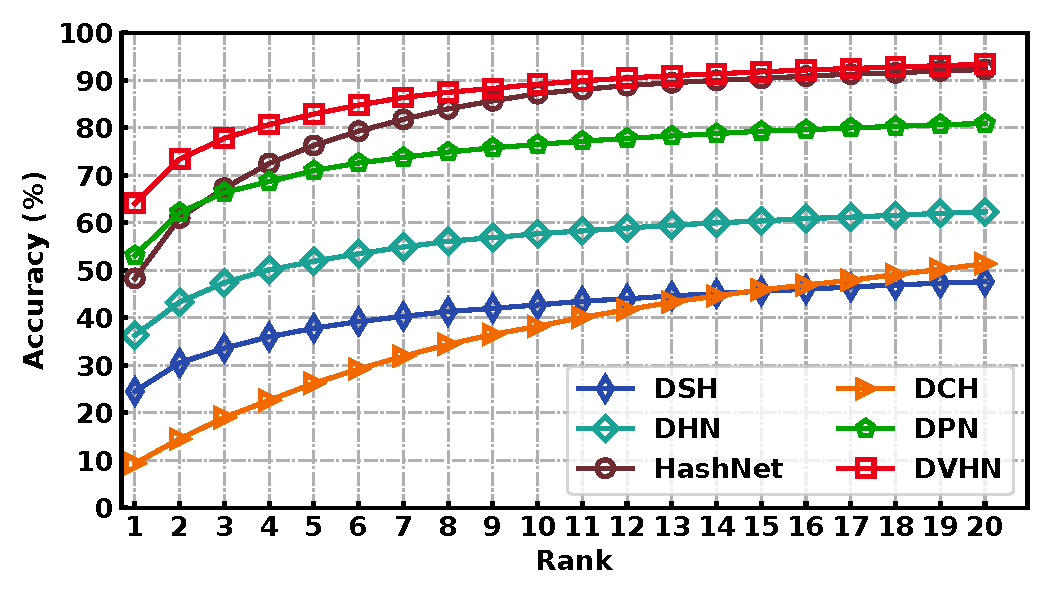
\includegraphics[width=13cm]{03/vid_1600_2048.pdf} \\
    \bicaption[在\textbf{VehicleID (1600)}上2048位的哈希算法的CMC结果]
    {2048位哈希算法在\textbf{VehicleID (1600)}上的结果}
    {CMC Results on \textbf{VehicleID (1600)} of 2048 bits}
   \label{fig:vid1600_2048}
  \end{figure}
  
  \begin{figure}[!htp]
    \centering
    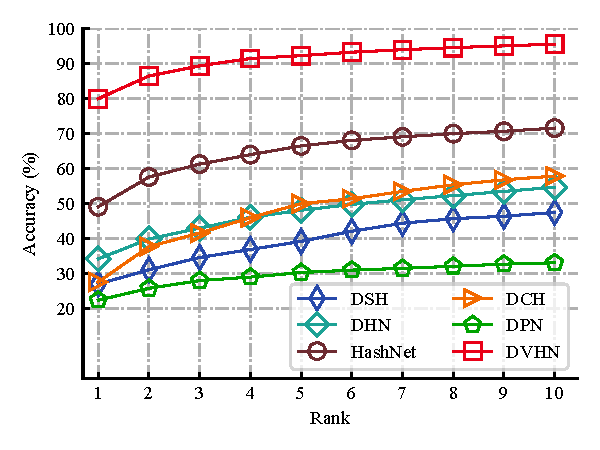
\includegraphics[width=13cm]{03/veri_256.pdf} \\
    \bicaption[在\textbf{VeRi}上256位的哈希算法的CMC结果]
    {256位哈希算法在\textbf{VeRi}上的结果}
    {CMC Results on \textbf{VeRi} of 256 bits}
   \label{fig:veri256}
  \end{figure}
  \begin{figure}[!htp]
    \centering
    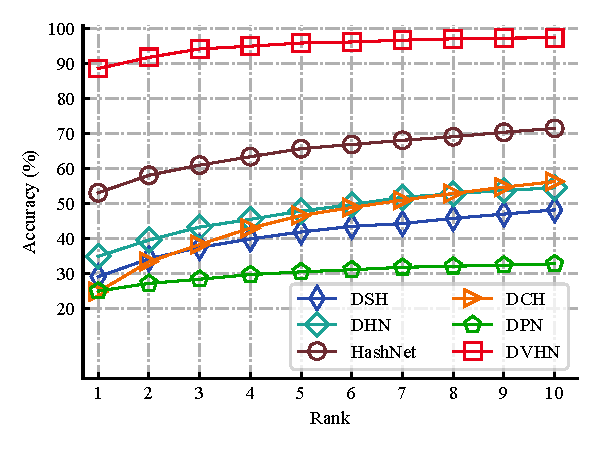
\includegraphics[width=13cm]{03/veri_2048.pdf} \\
    \bicaption[在\textbf{VeRi}上2048位的哈希算法的CMC结果]
    {2048位哈希算法在\textbf{VeRi}上的结果}
    {CMC Results on \textbf{VeRi} of 2048 bits}
   \label{fig:veri2048}
  \end{figure}




另外, 我们也加入其他的最近的哈希方法进行细致的比较和分析, 包括~\textbf{DHN}~\cite{zhu2016deep}, \textbf{HashNet}~\cite{cao2017hashnet}, \textbf{DCH}~\cite{cao2018deep}, \textbf{DPN}~\cite{fan2020deep}。值得注意的是对于~\textbf{SH}, ~\textbf{ITQ},~\textbf{DCH}和~\textbf{DHN}我们采用作者开源的代码, 而对于其他的方法, 我们基于\textit{Pytorch}进行重新实现。我们首先对于所有的模型在生成哈希码为$2048$位的情况下进行分析。如表~\ref{table:vid800}, 表~\ref{table:vid1600}和表~\ref{table:veri}所示, 很明显, 传统的非深度学习的方法如~\textbf{SH}和~\textbf{ITQ}在两个数据集上都只能取得显著较低的性能。在哈希码长度为$2048$位是, 它们在\textbf{VeRi}数据集上分别取得$1.57\%$和$5.14\%$ \textbf{mAP}。 在\textbf{VehicleID (800)}和\textbf{VehicleID (1600)}上, 性能稍微有上升的趋势。具体来说, \textbf{SH}取得了$17.71 \%$ 和 $13.83 \%$ \textbf{mAP}而 \textbf{ITQ}分别达到了$26.26 \%$ 和 $22.23\%$。
\begin{figure}[!htp]
    \centering
    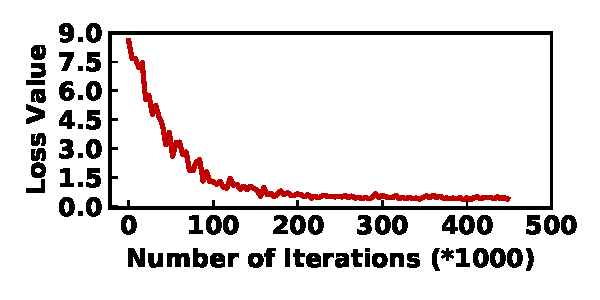
\includegraphics[height=3.5cm]{03/loss_256.pdf}
    \hspace{1cm}
    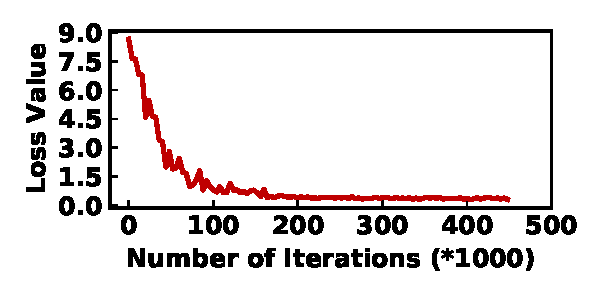
\includegraphics[height=3.5cm]{03/loss_512.pdf}
    \bicaption[\textbf{DVHN}在$256$和$512$哈希长度下的收敛图]{\textbf{DVHN}在$256$ (左)和$512$ (右)哈希长度下的收敛曲线}{The convergence curve of \textbf{DVHN} on 256 (left) and 512 (right) bits.}
    \label{fig:losscurve}
  \end{figure}

  \begin{figure}[!htp]
    \centering
    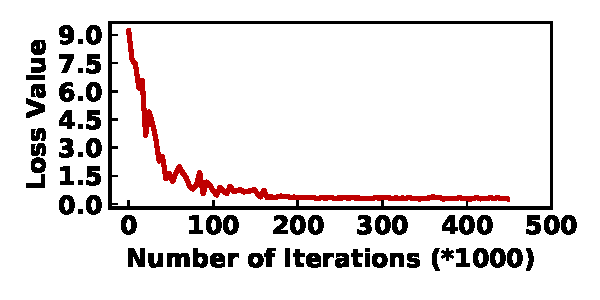
\includegraphics[height=3.5cm]{03/loss_1024.pdf}
    \hspace{1cm}
    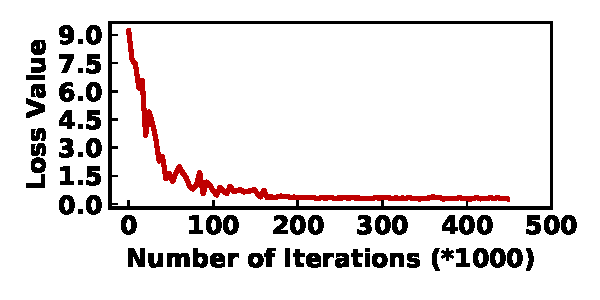
\includegraphics[height=3.5cm]{03/loss_2048.pdf}
    \bicaption[\textbf{DVHN}在$1024$和$2048$哈希长度下的收敛图]{\textbf{DVHN}在$1024$ (左)和$2048$ (右)哈希长度下的收敛曲线}{The convergence curve of \textbf{DVHN} on 1024 (left) and 2048 (right) bits.}
    \label{fig:losscurve1}
  \end{figure}


性能不优的主要原因是无监督的方法难以学习到具有判别力的特征, 从而导致了次优的哈希码。很明显, 监督的方法在两个数据集上在四种不同哈希码长度上都能取得更加优秀的结果。具体来说, ~\textbf{HashNet} 和 \textbf{DPN} 在\textbf{VehicleID (800)}上取得了优异的性能, 在 $2048$位的情况下分别取得 $66.61 \%$ 和 $64.65 \%$ \textbf{mAP}。对于其他哈希长度来说, 在\textbf{mAP} 这个指标下, 他们也是明显的赢家。 对于\textbf{VeRi}数据集, 两种算法的性能出现了明显的下降, 对于\textbf{HashNet}和\textbf{DPN} 分别取得 $29.30\%$ 和$13.58\%$。 性能的下降主要是由于\textbf{VeRi} 数据集是现实数据集, 有较大的背景遮挡, 视角变化等等带来的检索难度的提升。很明显, 本章提出的框架-\textbf{DVHN}对与所有的哈希长度以及在所有的测试数据集下都是优胜者。具体上, ~\textbf{DVHN}在$2048$位时, 在\textbf{VehicleID} 和\textbf{VeRi}上对于最先进的结果取得$11.05\%$和$35.46 \%$的\textbf{Rank-1}准却度提升。



对于$256$位的场景, 在两个数据集上, 我们获得了$11.54 \%$ 和 $30.93 \%$的提升。对于~\textbf{mAP}而言, 在$2048$位的哈希码长度场景下, 我们在\textbf{VehicleID (800)}, \textbf{VehicleID (1600)} 和 \textbf{VeRi}上, 我们分别取得了$76.82 \%$, $72.72 \%$ 和 $56.58 \%$。相比较次优的方法而言, 我们获得了$10.21 \%$, $11.30 \%$和$32.72\%$的性能提升。优越的性能可以证实我们的同时哈希和分类的设计可以使得模型学习到更具有判别性的特征, 生成更加紧凑的编码。\par 
我们额外提供了 各个模型在不同的哈希长度情况下在~\textbf{VehicleID (800)}, ~\textbf{VehicleID (1600)}和~\textbf{VeRi}三种数据集下的\textbf{top-K} 准确度的结果(CMC 曲线), 如图~\ref{fig:vid256}, 图~\ref{fig:vid2048}, 图~\ref{fig:vid1600_256}, 图~\ref{fig:vid1600_2048} 以及图~\ref{fig:veri256} 和图~\ref{fig:veri2048}所示。 \par
\textbf{VehicleID (800):} 如图~\ref{fig:vid256}和图~\ref{fig:vid2048}所示, 本章比较了~\textbf{DVHN}和其他深度哈希模型在不同的哈希长度下的 \textbf{top-K}准确度差异。值得注意的是, 由于无监督算法较低的性能表现, 我们并没有加入无监督的哈希算法进行比较。很明显可以发现, 在\textbf{Rank-1}到\textbf{Rank-5}, \textbf{DVHN}都取得了非常显著的性能提升。相比较~\textbf{DPN}而言 ~\textbf{DVHN}在$256, 512, 1024, 2048$ 哈希码长度的场景下分别取得取得了$11.52\%,~9.61\%,~10.75\% $和 $11.05\%$ 的性能提升。同时也能发现, ~\textbf{HashNet} 在\textbf{Rank-6}到\textbf{Rank-10}下也能取得比较优异的结果。然而在重识别任务中, 返回的匹配图片越靠前越满足检索需求。同时也能发现, 我们的模型在哈希码长度增加时能取得更加优异的结果, \textbf{mAP}从$71.61\%$提高到$76.81$。性能的提升主要归功于较长的哈希码可以保存更多的相似度信息。 \par


\begin{figure}[!htp]
    \centering
    \begin{subfigure}{\textwidth}
      \centering
      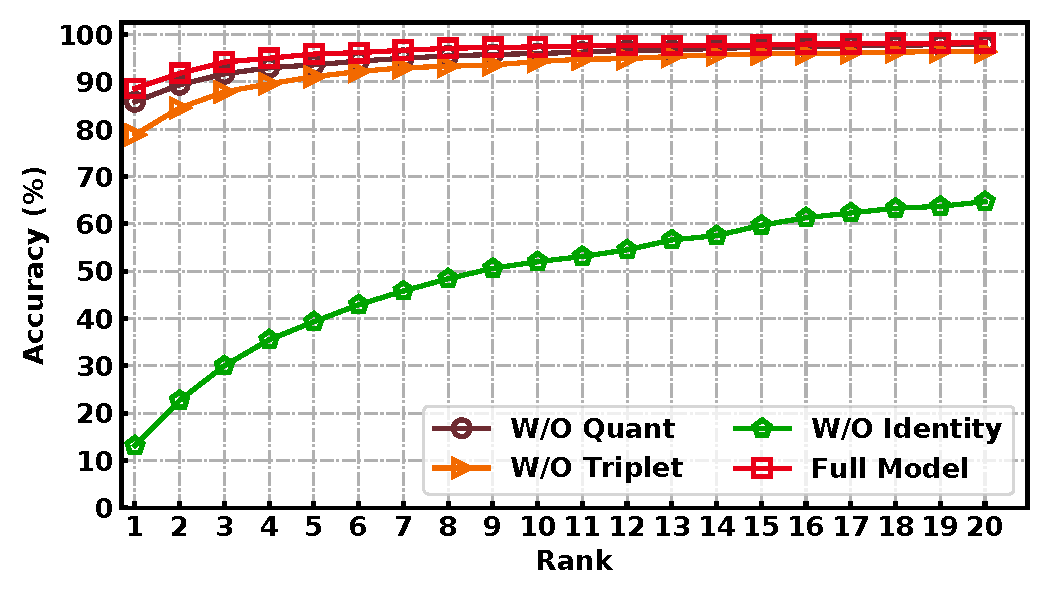
\includegraphics[height=8cm]{03/ablation_veri.pdf}
      \caption{不同的变种在\textbf{VeRi}数据集上的\textbf{CMC}曲线}
    \end{subfigure}
    \hspace{1cm}
    \begin{subfigure}{\textwidth}
      \centering
      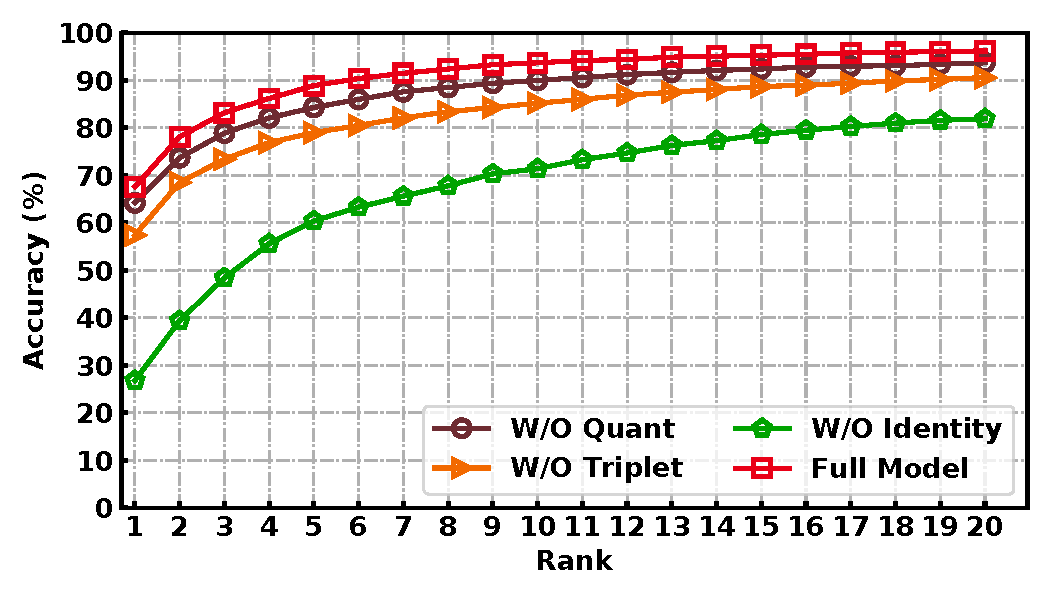
\includegraphics[height=8cm]{03/ablation_vid.pdf}
      \caption{不同的变种在\textbf{VehicleID}数据集上的\textbf{CMC}曲线}
    \end{subfigure}
    \bicaption[\textbf{DVHN}消融实验的\textbf{CMC}结果]{\textbf{DVHN}消融实验的在\textbf{VehicleID (800)} 和\textbf{VeRi}数据集上的\textbf{CMC}结果}{The ablation results on \textbf{VehicleID (800)} and \textbf{VeRI} of \textbf{DVHN}}
    \label{fig:ablationcmc}
  \end{figure}

\textbf{VehicleID (1600):}对于在这个场景下的性能表现, 如表~\ref{table:vid1600}, 图~\ref{fig:vid1600_256}和图~\ref{fig:vid1600_2048}所示, 在\textbf{CMC}和\textbf{mAP}上我们可以发现相似的趋势。\textbf{DVHN}在$256, 512, 1024$和$2048$位场景下可以取得$57.06\%, 60.41\%, 63.26\% $ $64.11\%$的\textbf{Rank-1}性能。对于\textbf{mAP}, \textbf{DVHN}可以在所有场景下均取得了大范围的性能提升。值得注意的是, 与\textbf{VehicleID (800)}的测试相比, 模型的性能有明显的下降。 例如, \textbf{Rank-1}准确度在哈希码长度为$256$位时, 下降了接近$5 \%$。这主要是由于数据库中照片增大导致的检索难度提升。 \par
\textbf{VeRi: }如表~\ref{table:veri}和图~\ref{fig:veri256}以及图~\ref{fig:veri2048}所示, \textbf{DVHN}和其他所有比较的方法在所有的评估指标上都显示出了持续的优势。 如图~\ref{fig:veri256}以及图~\ref{fig:veri2048}所示, ~\textbf{DVHN}大幅度领先\textbf{HashNet}。我们在$256,512,1024,2048$位哈希码的场景分别获得了$80.10\%, 85.81\%, 87.01\% $和 $88.62\%$的\textbf{Rank-1}准确度, 比~\textbf{HashNet}对应超出$30.93\%, 33.85\%, 33.73\%$ 和 $35.46\%$。对于~\textbf{mAP}而言, \textbf{DVHN}和其余比较的方法的性能差异更加显著。我们比第二优的方法在$2048$位的哈希码场景下超出了$32.77 \%$。明显, 在图~\ref{fig:veri256}以及图~\ref{fig:veri2048}中, 代表~\textbf{DVHN}性能的红色曲线持续在其他曲线之上, 并且以大幅度领先。我们算法的优越性可以归功于我们的相似度保留的学习策略和离散哈希的模块的紧耦合的设计。

\begin{figure}[!htp]
    \centering
    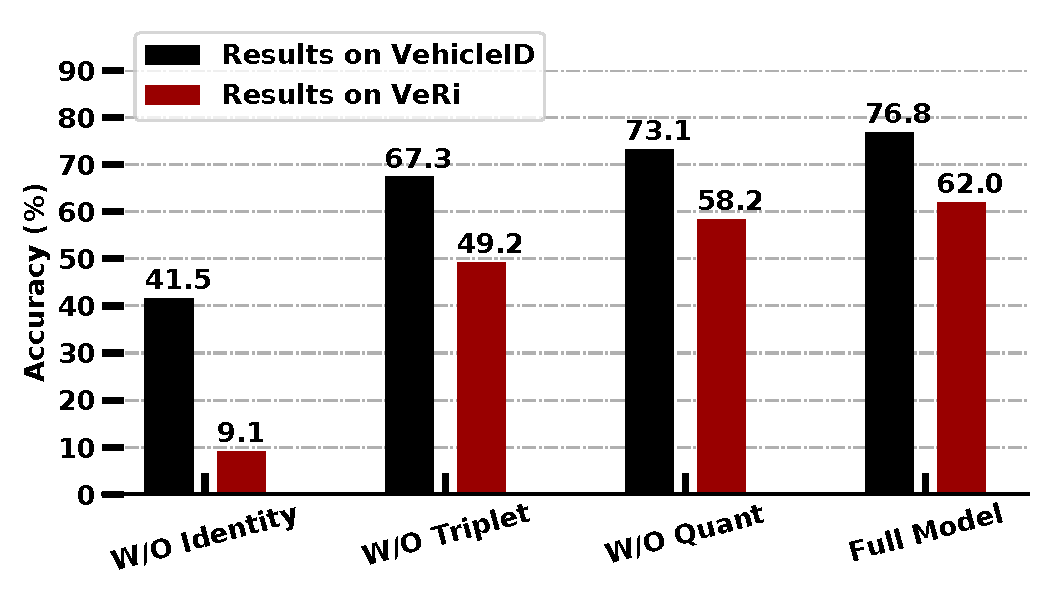
\includegraphics[width=15cm]{03/ablation_map.pdf} \\
    \bicaption[在\textbf{VehicleID (800)}和\textbf{VeRi}数据集上的消融实验\textbf{mAP}结果]
      {不同的变种在\textbf{VehicleID (800)}和\textbf{VeRi}数据集上的\textbf{mAP}}
      {The ablation results on \textbf{VehicleID (800)} and \textbf{VeRI} in terms of \textbf{mAP}}
   \label{fig:ablationmap}
\end{figure}

\subsection{经验性分析}
首先, 本章的模型在不同哈希长度下的收敛曲线如图~\ref{fig:losscurve}和图~\ref{fig:losscurve1}所示。\par
其次, 我们进行的详细的消融实验来证明\textbf{DVHN}框架中各个组成部分的效果。为了有效的评估身份损失函数$L_{Identity}$, 基于三元组的损失函数$L_{Triplet}$和我们设计的离散学习损失$L_{Quant}$, 我们设计了如下变种算法, 并且依次测试了他们在\textbf{VehicleID (800)}和\textbf{VeRi}数据集上的性能。
\begin{enumerate}
    \item \textbf{Full Model:} 一个包含了全部的部件的变种模型, 也就是完整版的\textbf{DVHN}。
    \item \textbf{W/O Triplet:} 缺少了基于三元组的相似度保留损失函数$L_{Triplet}$的模型。 
    \item  \textbf{W/O Identity:} 缺少了基于分类器的分类损失函数$L_{Identity}$的变种模型。
    \item \textbf{W/O Quant:} 缺少了离散哈希学习模块的变种模型。
\end{enumerate}
值得注意的是, 所有的消融实验是在哈希码为$2048$位的情况下进行。如图~\ref{fig:ablationcmc}和图~\ref{fig:ablationmap}所示, 


\begin{figure}[!htp]
    \centering
    \begin{subfigure}{\textwidth}
      \centering
      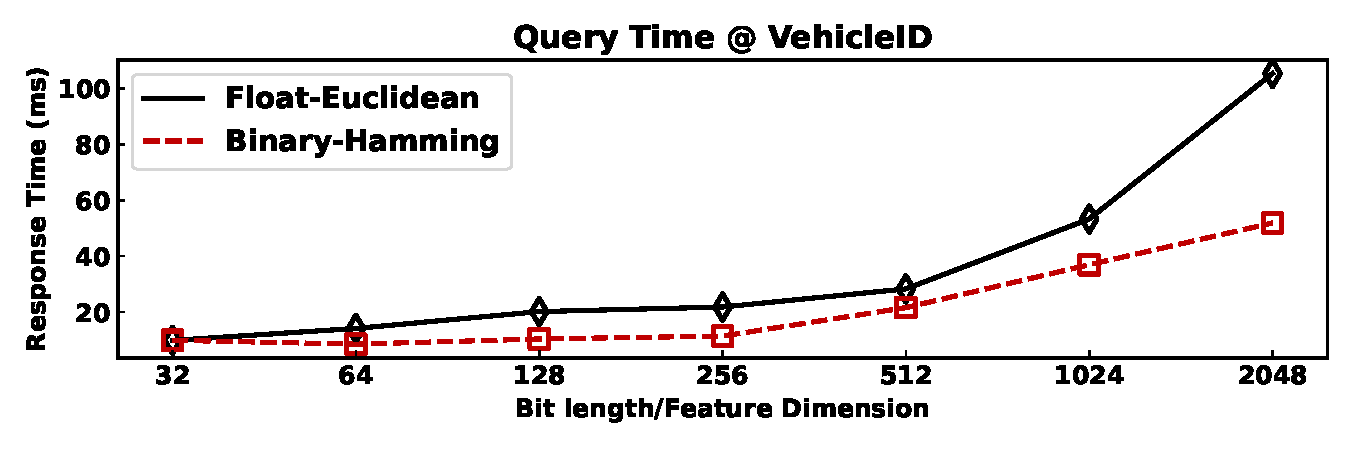
\includegraphics[height=4cm]{03/vehicle_query_speed.pdf}
      \caption{在\textbf{VehicleID}上的查询时间}
    \end{subfigure}
    \hspace{1cm}
    \begin{subfigure}{\textwidth}
      \centering
      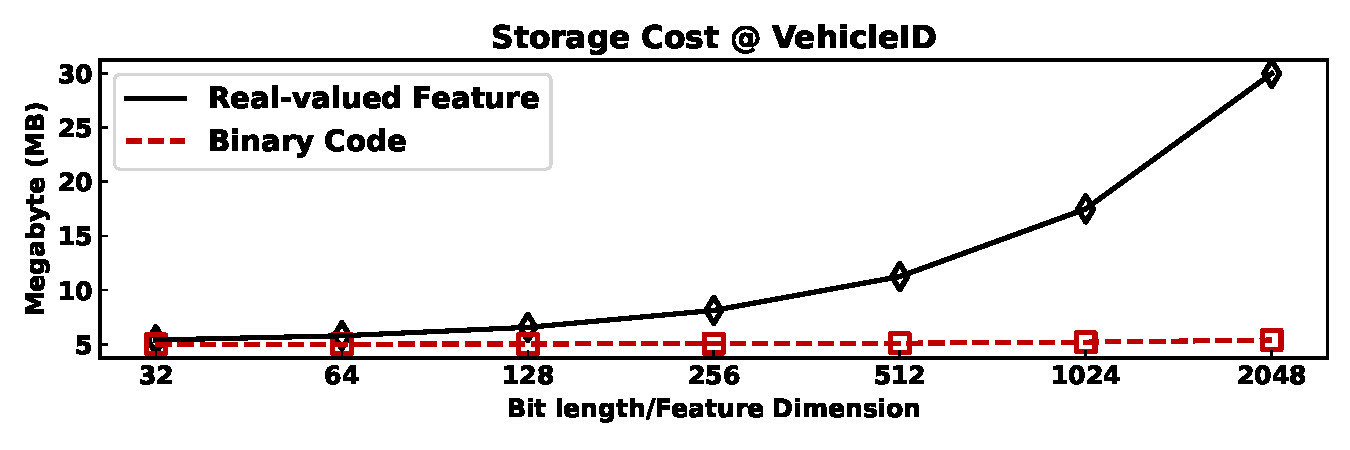
\includegraphics[height=4cm]{03/vehicle_storage.pdf}
      \caption{在\textbf{VehicleID}上的存储开销}
    \end{subfigure}
    \begin{subfigure}{\textwidth}
        \centering
        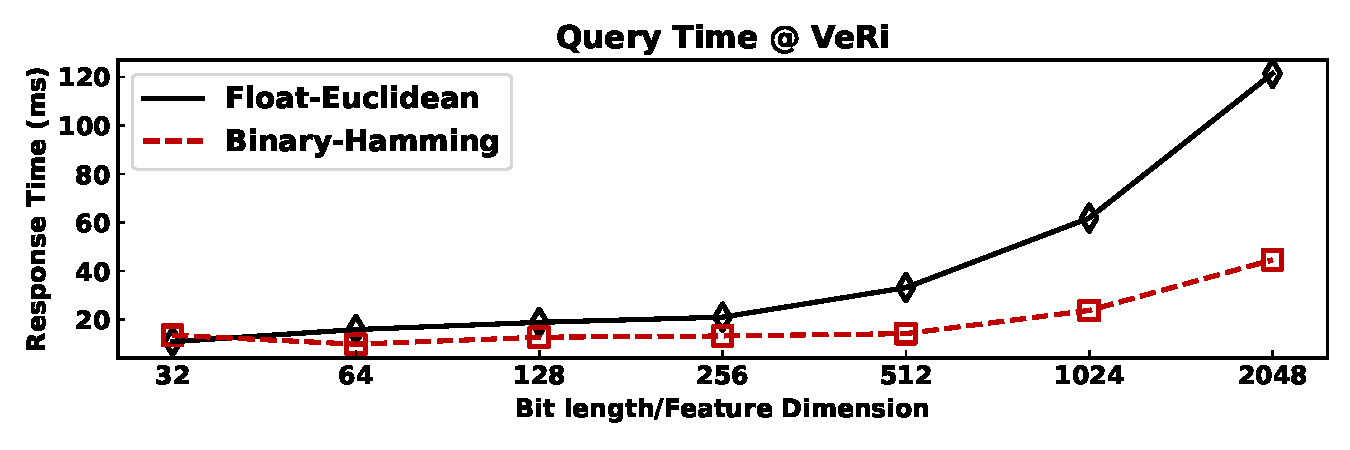
\includegraphics[height=4cm]{03/veri_query_speed.pdf}
        \caption{在\textbf{VeRi}上的查询时间}
      \end{subfigure}
      \begin{subfigure}{\textwidth}
        \centering
        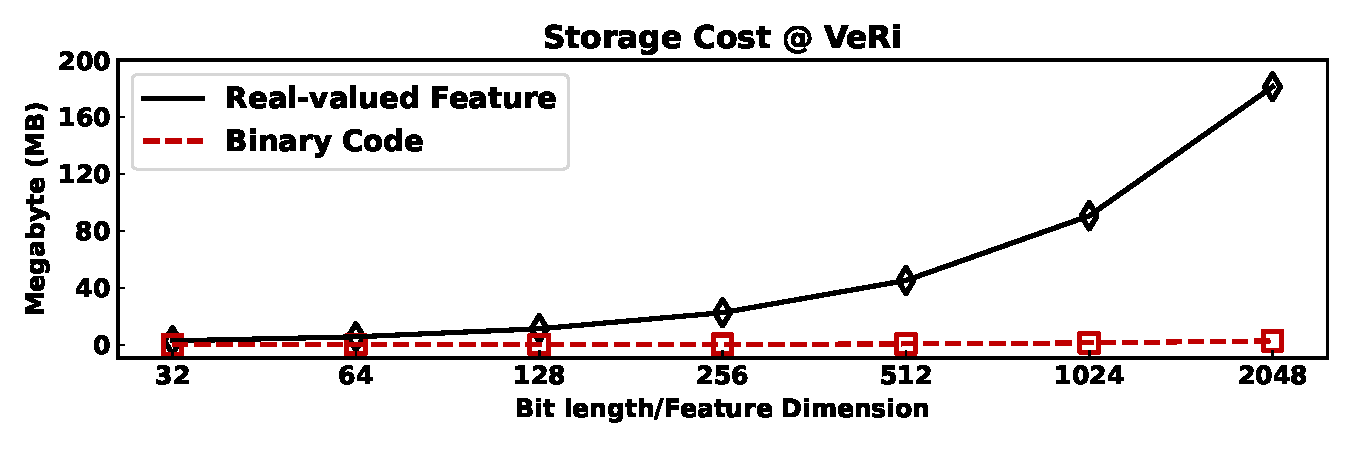
\includegraphics[height=4cm]{03/veri_storage.pdf}
        \caption{在\textbf{VeRi}上的存储开销}
      \end{subfigure}
    \bicaption[存储开销和查询时间的对比]{实值检索和基于哈希码的检索的存储开销和检索时间对比}{Comparison of the total query response time and storage cost of real-valued vectors and binary hash code}
    \label{fig:sttcost}
  \end{figure}
  当模型没有离散学习损失函数时, \textbf{Rank-1}准确度 和 \textbf{mAP} 在\textbf{VehicleID (800)}数据集上分别下降$3.46 \%$ 和 $3.50 \%$, 而在\textbf{VeRi}数据集上分别下降$2.80 \%$和$3.77 \%$。这证实了本章提出的离散学习模块在生成包含车辆信息的二进制编码的有效性。当模型失去$L_{Identity}$, 如图中的 \textbf{W/O Identity}所示, 模型的性能遭遇了显著的下降。具体来说, 在\textbf{VehicleID (800)}上, \textbf{Rank-1}准确度下降了$40.84 \%$而\textbf{mAP}则下降了$35.31 \%$。 在\textbf{VeRi}数据集上, 性能的下降更加的显著, \textbf{Rank-1}准确度下降了$75.11 \%$而\textbf{mAP}则下降了$52.84 \%$。性能的大幅度下降也证实了身份损失函数在学习强健并且有判别性特征方面的重要性。最后, 当我们观察没有了$L_{Triplet}$损失函数的橙色曲线\textbf{W/O Triplet}, 我们也可以观察到和\textbf{Full Model}对比的显著的性能下降。在\textbf{VehicleID (800)}上, \textbf{W/O Triplet}取得了$57.47 \%$的\textbf{Rank-1} 准确度和$67.32 \%$ 的\textbf{mAP}, 比\textbf{Full Model}分别下降了$10.19 \%$和$9.45 \%$。在\textbf{VeRi}数据集上, 我们也能观察到类似的趋势。\textbf{W/O Triplet}获得了$78.84$ \% \textbf{Rank-1}准确度和$49.23 \%$的\textbf{mAP}, 比\textbf{Full Model}降低了$9.78 \%$ 和 $12.79\%$。 模型性能的下降主要可以证明基于困难三元组的三元损失函数在解决车辆重识别问题的有效性, 特别是在类内变化有时候比类间变化更显著情况下。由此小节的消融实验可以证明各个部分的损失函数对于\textbf{DVHN}模型的整体性能都是不可缺少的。 
  
\begin{figure}[!htp]
    \centering
    \includegraphics[width=15.5cm]{03/256_retrieved_results.pdf} \\
    \bicaption[256位的\textbf{DVHN}框架的检索结果可视化]
      {256位的\textbf{DVHN}框架在\textbf{VehicleID (800)}数据集上的的前十检索结果可视化}
      {The Visualization of the Top 10 Retrieved Results of \textbf{DVHN} Framework on 256 Hashing Bit}
   \label{fig:retrieval256}
\end{figure}
\subsection{检索效率比较}
车辆重识别 (Vehicle ReID)系统的检索时间开销一般分为两个部分: ``特征提取的时间开销''和``向量距离计算的时间开销''。如Chen等人~\cite{chen2020deep}指出, 特征提取的时间开销其实绝大部分和使用的主干神经网络相关, 我们在固定使用同样的神经网络模型。 在本小节的比较中, 我们主要关注比较我们方法的大规模的距离计算的时间开销和基于实值向量的大规模计算的开销。 同时, 我们也和基于实值向量的方法比较我们基于二进制汉明哈希码的存储开销。\par
如图~\ref{fig:sttcost} 所示, 我们展示了在\textbf{VehicleID (1600)}和\textbf{VeRi}上的检索效率对比。 其中\textbf{VehicleID (1600)}包含$11,777$张查询图片, $1,600$张数据库照片, 而 \textbf{VeRi}包含了$1,678$张查询图片和$11,579$张数据库照片。在图~\ref{fig:sttcost}中a和c, ``Float-Euclidean''表示基于实值向量的车辆重识别方法在数据集上进行大规模欧式距离计算的时间开销。而``Binary-Hamming''表示基于二进制哈希码的车辆重识别方法在数据集上进行大规模汉明距离计算的时间开销。对于图(c)和图(d), 其展示了两种不同的方法在两个数据集上不同的向量长度的存储开销。 非常明显可以看出基于二进制哈希码的方法可以大量降低存储的开销以及提高检索的速度。
\begin{figure}[!htp]
    \centering
    \includegraphics[width=15.5cm]{03/512_retrieved_results.pdf} \\
    \bicaption[512位的\textbf{DVHN}框架的检索结果可视化]
      {512位的\textbf{DVHN}框架在\textbf{VehicleID (800)}数据集上的的前十检索结果可视化}
      {The Visualization of the Top 10 Retrieved Results of \textbf{DVHN} Framework on 512 Hashing Bit}
   \label{fig:retrieval512}
\end{figure}
\begin{figure}[!htp]
    \centering
    \includegraphics[width=15.5cm]{03/1024_retrieved_results.pdf} \\
    \bicaption[256位的\textbf{DVHN}框架的检索结果可视化]
      {1024的\textbf{DVHN}框架在\textbf{VehicleID (800)}数据集上的的前十检索结果可视化}
      {The Visualization of the Top 10 Retrieved Results of \textbf{DVHN} Framework on 1024 Hashing Bit}
   \label{fig:retrieval1024}
\end{figure}
\begin{figure}[!htp]
    \centering
    \includegraphics[width=15.5cm]{03/2048_retrieved_results.pdf} \\
    \bicaption[256位的\textbf{DVHN}框架的检索结果可视化]
      {2048位的\textbf{DVHN}框架在\textbf{VehicleID (800)}数据集上的的前十检索结果可视化}
      {The Visualization of the Top 10 Retrieved Results of \textbf{DVHN} Framework on 2048Hashing Bit}
   \label{fig:retrieval2048}
\end{figure}
\subsection{车辆检索结果的定性分析}
在图~\ref{fig:retrieval256}, 图~\ref{fig:retrieval512}, 图~\ref{fig:retrieval1024}和图~\ref{fig:retrieval2048}中, 我们可视化\textbf{DVHN}再不同的哈希码长度的场景在\textbf{VeRi}数据集上的检索结果。为了展示检索的有效性, 我们将原先的数据库集当成查询集, 将查询集当作被检索的数据库集, 这样的话每一张查询的图片在数据库中有多个对应的图片。在上述的可视化图中, 为了方便对比性能, 我们采用同一张查询的图片在$256$, $512$, $1024$, $2048$四个长度的哈希码场景下进行检索。图的右侧可视化了对于查询图片生成的前十张检索图片。蓝色框圈出来的图片代表它和查询图片是属于同一辆车。通常来说, 对于一个重识别的模型, 我们希望在检索返回的图片中属于同一辆车的图片尽量靠前。在四张可视化图中也可以看出来, $2048$位的哈希检索模型有更加的检索效果。
\subsection{总结}
本章基于深度哈希学习提出了第一个进行高效大规模车辆重识别的框架-\textbf{DVHN}。受深度哈希采用二进制哈希码来进行高效的检索的启发, 我们进行第一个引入二进制哈希算法进行解决大规模车辆重识别问题, 和传统基于实值的检索方法相比, 极大的的降低了存储的开销以及提高了检索的速度。具体来说, 对于相似度保持的度量学习, 本章采取了一个三元损失函数以及一个设计了在线困难三元组生成模块。同时, 我们额外增加了一个基于分类损失的身份损失函数来学习更强健和有判别性的特征表示。 对于二进制码学习, 我们基于二进制码应该尽量保留图像的类别信息的假设, 提出了一个离散哈希学习方法。 为了解决由于生成二进制码使用\textit{sign}函数带来的梯度消失的难题, 我们提出一个交叉优化的方法来优化整个框架。我们在标准的大规模车辆数据集上进行了大规模广泛的实验。 实验结果表明本章提出的框架~\textbf{DVHN}可以生成有效的二进制哈希码来进行大规模的车辆检索, 并且相比较当前的其他先进的深度哈希方法, 我们的方法可以大幅度的提升检索的精度。


% !TEX root = ../main.tex
\chapter{基于Vision Transformer的深度哈希检索模型}
由于其检索的速度以及较低的内存开销, 深度哈希在大规模图像检索领域获得了广泛的关注。直到本章的算法提出前, 这个领域的所有的深度哈希模型都是基于卷积神经网络而设计, 例如, \textbf{ResNet}~\cite{he2016deep}, \textbf{AlexNet}等。在本章中, 受最近Vision Transformer架构的启发, 我们设计了第一个完全基于Vision Transformer的深度哈希架构来进行大规模的图像检索。具体来说, 我们的架构包含两个基本的模块: (1) 基于Vision Transformer (ViT), 我们设计了一个孪生Vison Transformer的主干架构来进行特征提取。为了学习细粒度的特征, 我们设计了一个双流特征学习的Transformer块来同时学习局部和全局的特征。(2)同时, 我们采取一个基于动态创建的相似度矩阵作为监督标签设计的贝叶斯学习框架来学习相似度保持的紧凑的二进制哈希编码。整个框架是通过一种端到端的方法同一训练。据我们所知, 本章提出的深度哈希框架是第一个完全不基于卷积神经网络的深度哈希学习框架。本章的算法在三个被广泛研究的标准数据集上进行全方面的测试, 数据集包括:~\textbf{CIFAR-10},~\textbf{NUSWIDE},~和~\textbf{IMAGENET}。数据结果证实了我们的方法和现阶段的先进的深度哈希算法比较具有极高的性能的优越性。在三个数据集上, 我们比较第二优越的算法分别获得了 $8.2\%$, $2.6 \%$和$12.7\%$的性能增长。

\section{引言}
近些年来, 由于互联网技术的普及, 以及计算机技术, 便携摄像的进步, 传感器技术, 云计算以及各种社交网络的兴起, 由无数终端用户生成的视频和图片数据以爆炸性的速度增长。如何对海量的数据进行检索是利用数据进行其他大规模商业应用的基石, 因此准确和高效进行数据检索的研究开始受到学术界和工业界研究人员的大规模的关注。在这些技术研究中, 大规模图像检索由于其广泛的工业界应用, 如推荐系统, 搜索引擎, 遥感检索系统等, 受到了日益增长的关注。 在所有解决这一具有挑战性的任务的方法中\cite{fu2017fast, ge2013optimized, jegou2010product, malkov2018efficient}, 基于二进制码的哈希方法取得了令人瞩目的成果。基于哈希的方法通过学习一个哈希函数, 将高维像素空间中的图片映射到低维的二进制汉明空间中, 其中在低维度的汉明空间的图片对应的哈希码需要保存原图片之间的视觉相似性。过去的这些你那, 一大批的基于哈希的方法被提出。 根据它们提取特征的方法, 我们可以将其简单的分成两个类别: (1) 基于手工特征提取的方法 (2) 基于深度学习的方法。\par

\begin{figure}[!htp]
    \centering
    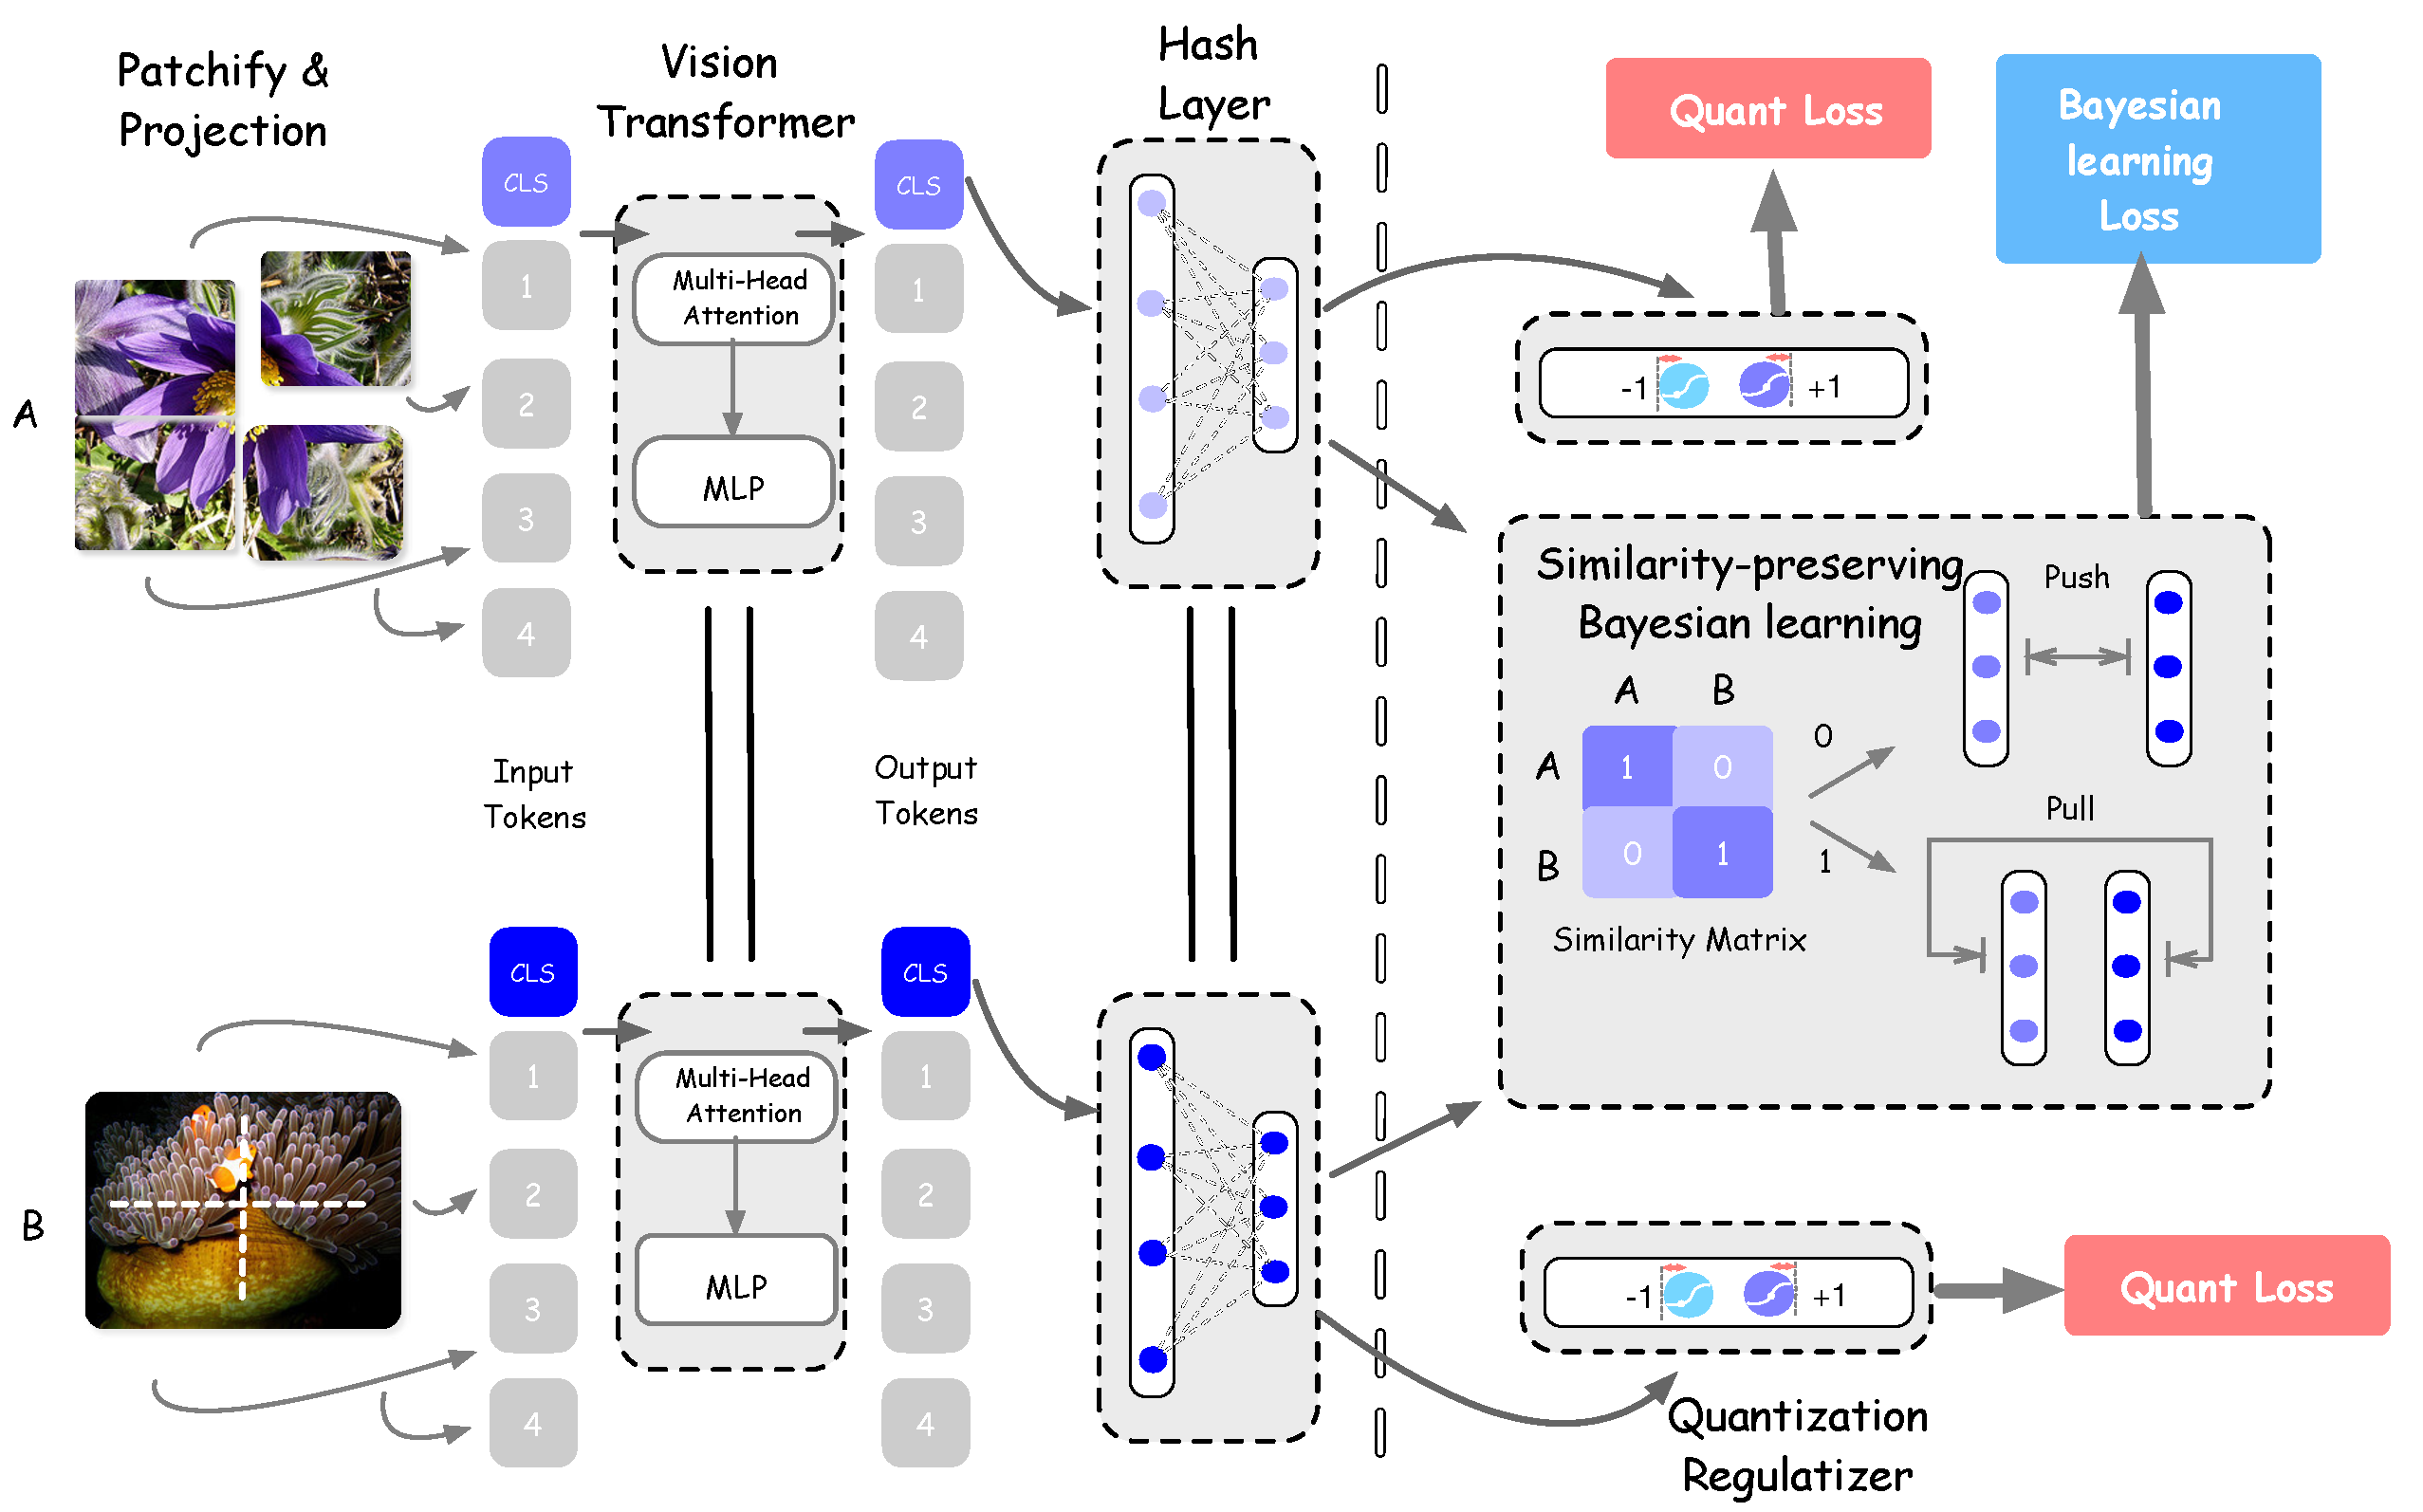
\includegraphics[width=15cm]{04/subfig.pdf} \\
    \bicaption[基于孪生Vision Transformer的图片检索基本框架]
      {对于一个图片对 (A, B), 我们将它们分割成固定大小的多个小图片块。然后将每个小块的像素转变成一个向量并且通过全连接将维成为一系列的嵌入表示。随后, 我们在这一系列的嵌入表征前添加一个随机初始化的向量作为分类嵌入。随后两串表征被输入进孪生Transformer模型并且通过一个哈希层生成$B$为的哈希向量。我们使用基于贝叶斯的学习框架来进行相似度保持学习。}
      {For an image pair (A,B), we cut them into several patches. Then every patch is flattened and projected to a fix-sized embedding with a fully connected layer, resulting in a sequence of embeddings. Subsequently, we add a classification token in the front of each sequence. Then, two sequences are fed into the Siamese transformer architecture. At last, we add a hash layer projecting the feature into B-bit hash vectors. The Bayesian learning module is employed to preserve the similarity in the \textit{Hamming} space for each pair. }
   \label{fig:subfig}
\end{figure} 

基于手工特征的浅层次哈希方法一般是通过基于人工设计的视觉特征描述符来进行哈希函数的学习~\cite{charikar2002similarity, indyk1997locality, weiss2008spectral}, 例如 \textbf{GIST}~\cite{oliva2001modeling}等。经典的浅层次哈希方法有~\textbf{LSH}~\cite{indyk1997locality}, 其主要思想是将相似的高维数据以比较大的概率被映射到相近的哈希编码中。然而由于基于手工提取的特征向量其实并不能准确的刻画保存原图片的有区别性的信息, 这导致了基于手工特征的哈希算法有一道无法逾越的性能鸿沟。为了减轻这个问题的影响, 随着AlexNet~\cite{}的提出, 基于深度学习的特征提取方法开始成为计算机视觉领域的主流。基于深度学习的模型~\cite{dosovitskiy2020image, russakovsky2015imagenet}相比较基于手工特征的方法通常而言可以获得显著的性能提升。基于深度学习的哈希学习方法一般包含两个阶段。 第一阶段致力于基于深度卷积神经网络, 例如 \textbf{AlexNet}等, 学习有判别性的特征。第二阶段包含包含设计各种非线性的函数来将连续性的神经网络输出转化成固定的哈希长度的二进制哈希码, 并且通过各种度量学习的损失函数~\cite{cakir2019hashing,cao2018deep,erin2015deep,gong2012iterative, li2015feature}来在汉明空间保存其对应的图片的视觉相似性。 \par
最近, Transformer~\cite{vaswani2017attention}模型展示了其在自然语言领域的卓越性能~\cite{brown2020language, devlin2018bert}。随后, Google设计了 Vision Transformer~\cite{dosovitskiy2020image}, 一种基于 Transformer的变种, 正式将Transformer引入进计算机视觉领域。Vision Transformer 开始在各个计算机视觉任务上超越传统基于卷积神经网络的模型(例如, 图像分类~\cite{dosovitskiy2020image}, 行人重识别~\cite{he2021transreid},等)。如图~\ref{fig:subfig}所示, Vision Transformer 通过首先将输入的图片分割成一系列的2D图片块。 随后, 将图片块转换成向量并且通过可以学习的转换矩阵来将向量将维度成低维度的特征表示。 随后, 一系列的输入向量可以被输入进标准的Transformer的编码器架构来学习特征表示。受Vision Transformer的高性能表现的启发, 我们思考完全基于Vision Transformer设计一个深度哈希框架的可行性。\par
在本章中, 我们基于Transformer 设计了一个新型的深度哈希框架-\textbf{TransHash}, 这是有史以来第一个不基于卷积神经网络作为主干网络来进行特征学习的深度哈希架构。具体而言, 为了进行成对的哈希学习, 我们设计了一个孪生多粒度Vision Transformer主干网络 (Multi-Granular Vision Transformer, MGVT)。它包含了两个完全一致的多粒度学习的Transformer网络, 并且这两个网络是完全共享所有参数~\cite{bromley1993signature}。具体而言, 为了进行多粒度的学习, 我们受\textbf{TransReID}~\cite{he2021transreid}所启发, 我们在传统的Vision Transformer的最后一层上设计了一个双流特征学习机制, 将最后一个Transformer块设计成两个并行的分支。对于第一个分支, 它是用来进行全局特征的学习。对于并行的第二个分支, 我们将前一个Transformer块的输出序列进行重新分组成$K$个序列组。这$K$个序列组的序列前都被添加了共享的用于分类的嵌入表征。随后, 将这$K$个序列分别输入进最后一个Transformer层来输出$K$个局部的特征。通过这样的方法, 我们可以通过全局和局部的网络架构设计同时学习到粗粒度的全局特征以及细粒度的局部特征。同时, 我们的模型还可以取得和Lai等人的工作~\cite{lai2015simultaneous}相似的效果。通过将哈希码的表征变成多个分支的哈希码的拼接, 类似于Lai等人提出的 divide-and-encode模块, 可以降低哈希码的冗余性。为了在特征空间保持原来图片的语义相似性, 我们提出采取基于贝叶斯学习的框架来将相似的图片对在特征空间中尽量拉近, 而将不相似的图片在特征空间中尽量拉远。最终, 由于基于卷积神经网络学习到的特征表示是连续的, 我们需要采用\textit{Sign}函数从将连续的表示生成离散的二进制哈希码。但是, 由于离散的哈希码$h$和连续的特征表示$f$之间存在鸿沟, 也就是``量化误差''~\cite{zhu2016deep}的存在, 直接在测试阶段使用\textit{sign}函数只能取得次优的检索性能。为了缩小量化误差, 减轻在测试阶段的性能损失, 我们将相似度保持学习重新规划成一个受限制的优化问题。具体做法是在之前的贝叶斯学习框架后加上一个科西分布量化损失来在训练阶段缩短连续的特征表示和二进制哈希码之间的差距。\par
总结而言, 本章做出了以下的创新与贡献:
\begin{enumerate}
    \item 本章设计了一个基于Vision Transformer的孪生多粒度Vision Transformer主干网络(Multi-Granular Vision Transformer, MGVT)。在传统的Vision Transformer的最后一层, 我们通过将其最后一层设计成一个并行的两个独立的分支, 设计一个新型的双流特征学习框架。 通过这种方法, 我们可以同时学习全局和局部的特征表示。同时, 如前所述, 它也可以进一步提高最后学习到的哈希向量各个位之间的独立性。
    \item 通过采用一个基于贝叶斯的相似度保持的贝叶斯学习模块以及一个量化损失的限制, 我们实现了第一个完全基于Transformer的深度哈希框架-\textbf{TransHash}来进行大规模的图像检索。据我们所知, 这是第一个不基于卷积神经网络的进行大规模图像检索的深度哈希框架。
    \item 我们在三个标准的检索数据集-\textbf{CIFAR-10}, \textbf{NUSWIDE} 和~\textbf{IMAGENET}-设计并且进行了一系列的全面的实验。实验结果表明了本章提出的框架-\textbf{TransHash}-具有优越的性能表现, 以大幅度领先当时的先进的深度哈希算法。
\end{enumerate}

\section{相关工作}
在本小节,~我们介绍与本章工作相关的其他工作。我们将相关的工作分为三个类别: (1) 在计算机视觉领域卷积神经主干网络的发展 (2) 在计算机视觉领域的Transformer的进展 (3)图像检索的深度哈希相关工作。
\subsection{计算机视觉领域的卷积神经网络发展}
卷积神经网络一开始是由LeCun 等人~\cite{cnnoriginal}提出来进行手写数字的自动识别。它提出了卷积核来对图片像素在空间区域的联系进行建模从而提取特征, 并且取得了显著的识别性能。然而直到2012年, \textbf{AlexNet}~\cite{alexnet}的提出, 基于卷积神经网络的方法才开始成为计算机视觉领域绝大部分任务的主要模型, 例如``实例分割''~\cite{he2016deep, ren2017end}, ``图像修复''~\cite{yeh2017semantic,yu2019free}, ``深度哈希''~\cite{cao2018deep, cao2017hashnet}, ``行人重识别''~\cite{chen2020maenet, hermans2017defense, ye2018hierarchical, ye2018visible} 等等。为了提高卷积神经网络的表征能力, 一系列更加深更加有效的卷积神经网络被提出。2014年, Simonyan and Zisserman~\cite{simonyan2014very} 提出了 VGG 网络。 VGG 从网络结构深度的角度来提升CNN的性能。通过使用3*3的小尺寸卷积核作为所有卷积层的标准, VGG 包括了最低11层到最高19层 (VGG-11、 VGG-13、 VGG-16、 VGG-19)等变种, 证明了提高模型的深度可以更好的学习图像中的视觉特征。 随后 GoogLeNet~\cite{szegedy2015going} 提出同时学习多尺度的图像特征。通过使用同时使用不同大小的卷积核(5*5、3*3、1*1)对图像进行卷积操作, 以及在通道维度进行拼接, 可以学习不同粒度的图像特征。在卷积神经网络发展的同时, 研究人员发现一味的增加卷积神经网络的深度在某个时候不能增加模型的性能, 甚至会导致梯度消失或者梯度爆炸等问题, 从而导致模型退化。为了解决这个难题, 2015年, Kaiming~\cite{he2016deep} 提出~\textbf{ResNet}, 通过恒等映射和残差映射来解决梯度消失的问题。从此,~\textbf{ResNet}开始成为计算机视觉领域的一个标准的基础主干神经网络。尽管基于卷积神经网络的模型目前任然在视觉领域占据主要的部位, 最近Vision Transformer的出现以及开启了采取Transformer的架构来进行一系列的视觉任务的可能性。本章提出的算法在当时是第一批利用Transformer来解决经典计算机视觉领域任务的工作。\par
\subsection{计算机视觉领域的Transformer发展}
Transformer最初是有2017年Google提出~\cite{vaswani2017attention}, 在自然语言处理领域进行序列数据的处理。从那时开始, 许多科研人员就开始在研究Transformer架构在计算机视觉领域的效果。最初的做法是利用Transformer处理由卷积神经网络提取的序列化的特征图~\cite{carion2020end, girdhar2019video, xie2021segmenting}。在2020年, Google提出了\textbf{Vision Transformer} (ViT) 通过将图片数据分块然后通过线性映射转换成一个序列的向量然后直接输入进传统的Transformer里通过在大型数据集上预训练后,就可以在多个任务如图像分类等领域取得了接近\textbf{ResNet}的性能。随后不同的ViT的变种开始在计算机视觉多个任务取得超越\textbf{ResNet}的性能效果。DeiT~\cite{touvron2021training}~是一个证实Transformer可以在中等大小的数据集上进行预训练并且取得较有的性能。DeiT通过使用CNN的输出当做一个教师模型, 通过蒸馏学习(distillation learning)来帮助训练自身的Transformer架构。在输入的嵌入表征前, 它们添加了一个蒸馏表征, 然后通过交叉熵损失和蒸馏损失进行训练。随后 Token-to-Token (T2T) Vision Transformer~\cite{yuan2021tokens}递归的将临近的token融合成一个token来降低序列的长度并且对于空间中的较远的联系进行建模。 Transformer in Transformer~\cite{han2021transformer}提出在两种层面上进行其中关键的注意力操作: (1) patch 层面, 与传统的ViT类似。 (2) 局部子patch层面, 通过将多个patch组合成一个大的子patch进行自注意力机制计算。通过这样的机制, 模型可以学习到更加细粒度的特征,~取得了更加优异的性能。由于ViT中d的自注意力机制的计算复杂度对于输入的序列长度而言是 $O(n^2)$, 这极大的限制了模型的可应用性。Pyramid ViT (PVT)~\cite{wang2021pyramid} 提出一个分层次的ViT设计, 通过逐步将整合临近的token缩小自注意力机制计算的序列长度。随后2021年的ICCV最佳论文~Swin Transformer~\cite{liu2021swin}通过将输入的图片块分成一个个限定大小窗口, 并且只在窗口内进行自注意力的计算。为了建立不同窗口内的patch之间的联系, 作者提出了一个Shifted Window分割机制, 在连续的两个Transformer层之间进行基于window的自注意力计算和shifted window的自注意力计算。Swin Transformer 在多个计算机视觉领域取得超越传统基于\textbf{ResNet-50}的模型, 开始成为取代卷积神经网络的计算机视觉主干深度神经网络。随后, CrossFormer
也基于一个分层次的Pyramid架构提出short-distance 注意力和long-distance 注意力, 在降低计算复杂度的同时可以同时捕捉局部和全局的特征信息。RegionVit~\cite{chen2021regionvit} 提出一个regional-to-local的注意力机制来对层次性特征进行编码。\par
除了上述基于ViT的基础主干网络的发展, 基于ViT的计算机视觉任务的应用也以惊人的速度增长。例如在``目标检测''任务中, Fang 等人提出~\cite{fang2021you}一个完全基于Transformer的目标检测框架。它将ViT中的用于分类的token替换成了多个可以学习的目标查询的token。在``图像分割''领域, Segmentation Transformer (SETR)~\cite{zheng2021rethinking} 使用ViT作为编码器, 使用两个解码器进行逐步的上采样。随后 SegFormer~\cite{strudel2021segmenter}~使用一个基于Pyramid ViT的编码器和一个简单的基于MLP的解码器来得到分割的掩膜。同样, Transformer在低层次视觉任务方面也取得了卓越的表现。在``图像处理''方面, chen 等人提出了一个基于预训练的Transformer模型。它可以进行多种图像修复的工作, 例如图像超分, 图像去噪, 等。除了在传统2D视觉领域, Transformer在3D计算机视觉方向也取得了令人瞩目的效果。3D点云的排序不变的特征天然适合Transformer的计算特性。2021年, Zhao 等人提出了 Point Transformer~\cite{zhao2021point} 提出了一个新型的点云Transformer层来对3D点的局部邻接信息进行自注意力计算。这个Transformer层基于向量自注意力机制, 其中的注意力权重是通过向量来表示。
Guo等人~\cite{guo2021pct}提出Pct来显式的对局部的3D结构进行编码, 并且在3D形状分类, 分割等领域取得了较好的性能表现。Lin等人提出一个Mesh Transformer~\cite{lin2021end}通过2D的图片重建3D得行人姿态以及进行网格重建, 这是第一个基于Transformer的3D行人重建的工作, 并且也取得了较好的结果。\par
Vision Transformer在此时仍然处于研究的初期, 并且由于其优越的性能得到了各个研究机构以及工业界的持续性上涨的关注。越来越多的研究人员在讲Vision Transformer引入进自己的研究方向来解决实际的问题。

\begin{figure}[!htp]
    \centering
    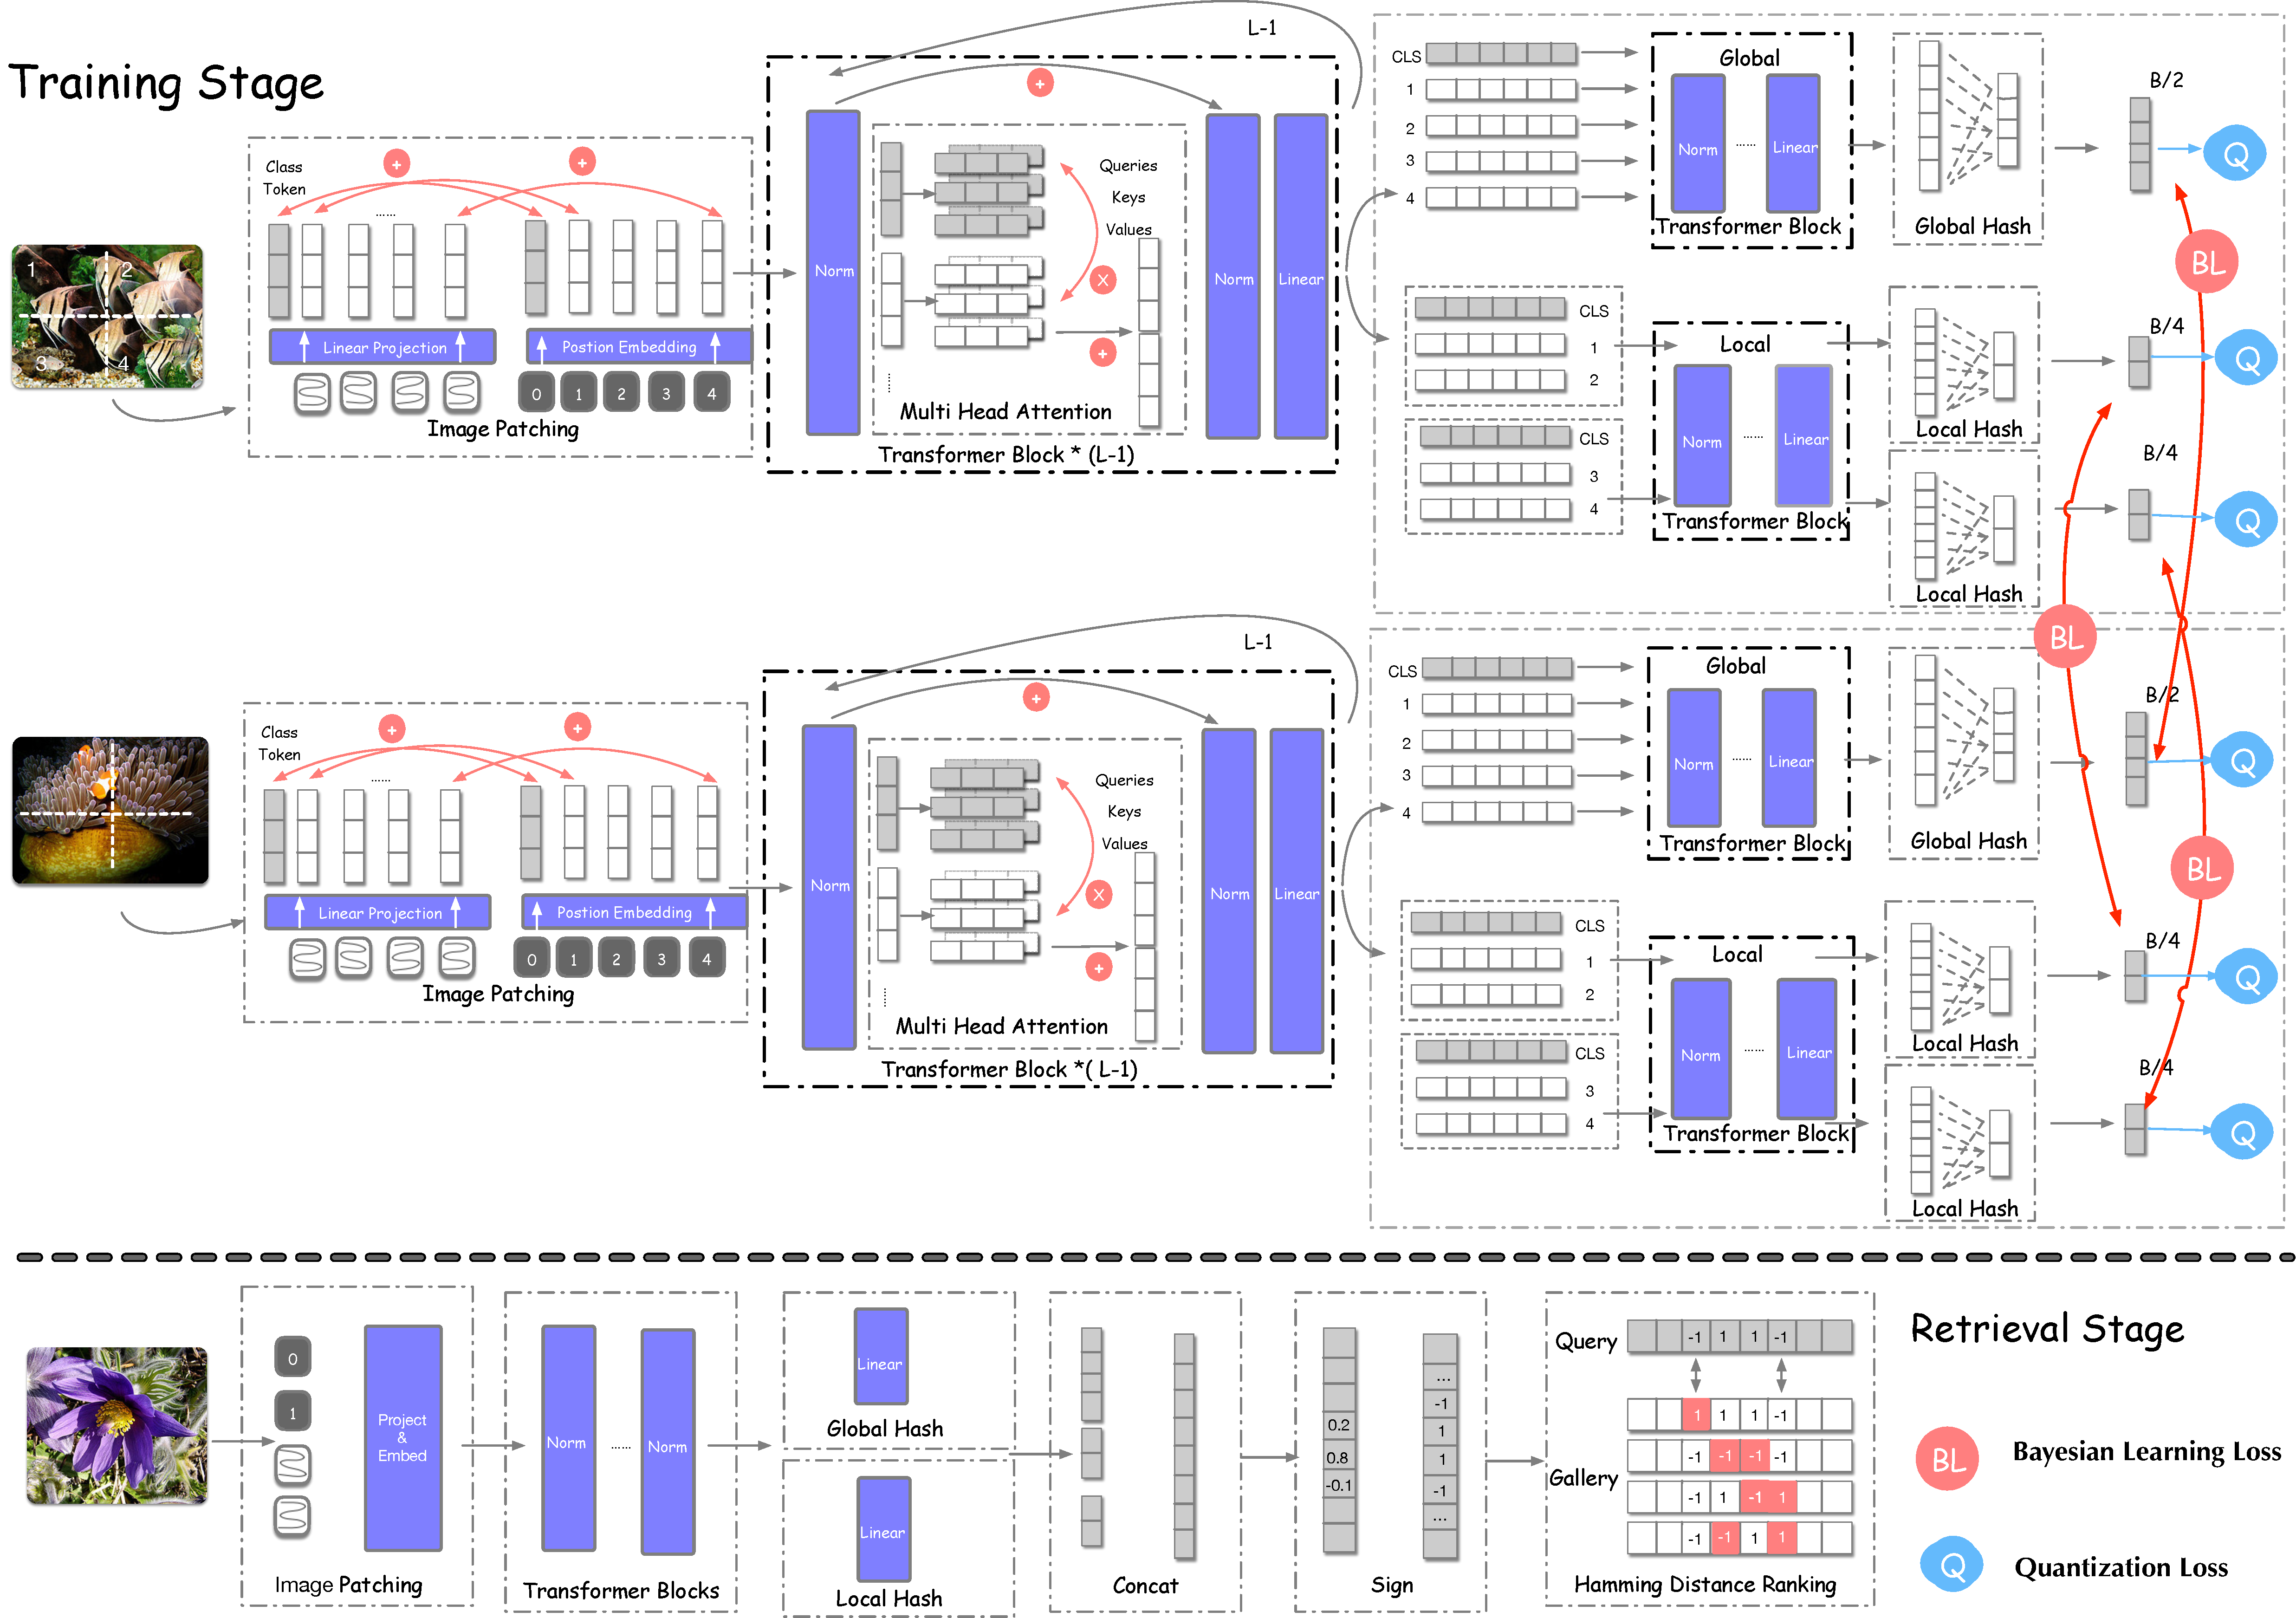
\includegraphics[width=15cm]{04/architecture.pdf} \\
    \bicaption[基于Vision Transformer的深度哈希框架]
      {TransHash的细节框架。图上部分表示了框架进行训练的阶段。我们采用一个孪生的架构。如传统的ViT, 输入图片将被切割成多个小块并且降维成一个序列的嵌入表征。在Transformer的最后一层, 我们设计了两个并行的Transformer 层来学习全局和局部的信息。同时, 对于全局和局部的特征, 我们均设计了对应的哈希层来进行哈希码的学习。 图的下部分表示测试阶段, 其中全局和局部的哈希码被连接成一个哈希码进行检索。}
      {The detailed architecture of the proposed \textbf{TransHash}. The upper part denotes the training stage. Specifically, we follow the same protocols as ViT by feeding the patch embedding together with the position embedding into the transformer encoder. At the last layer of the transformer, we design two parallel transformer blocks: global and local transformer blocks.  For the global feature and each local feature, we design a corresponding hashing layer. In the testing stage, the global and all the local hash vectors are concatenated and quantized into one hash code.}
   \label{fig:mainarch}
\end{figure} 

\subsection{基于哈希的图像检索}
深度哈希在大规模高效图像检索领域近年来获得了越来越多的关注~\cite{chen2021dvhn, ge2013optimized, gong2012iterative, heo2012spherical, indyk1997locality, yu2018product, weiss2008spectral}。根据它们提取特征的方法, 我们可以将它们分成两个类别: ``浅哈希方法''和``基于深度学习的哈希方法''。 \par
传统的浅哈希方法一般基于手工设计的特征来学习一个哈希函数将图片映射到二进制哈希码。一个典型的例子是~ Locality Sensitive Hash (LSH)~\cite{indyk1997locality}。LSH 致力于寻找一个哈希族使得相似的对象经过哈希函数产生的哈希碰撞要比不相似的概率要高。随后, Charikar等人~\cite{charikar2002similarity}提出另一个基于LSH的变种, SIMHASH, 其针对在欧式空间中的余弦相似性。 尽管这些基于手工特征的方法取得了一定程度的成功。 但是当应用到现实的数据时, 由于图片具有较多外观变化, 基于手工设计的特征并不能提取到有判别性的信息, 从而导致了哈希精度的不足。\par
基于这一点, 基于深度卷积神经网络提取特征进行哈希学习的方法研究取得了极大的进展~\cite{cao2017hashnet, fan20deep, li2015feature, liu2016deep, zhu2016deep}。2014年, Xia~\cite{xia2014supervised} 提出第一个基于深度学习的监督哈希框架。它提出一种两阶段哈希的方法先将相似度矩阵$S$ 分解成汉明矩阵$H$ 和 $H^T$的乘积, 其中 $H$的每一行代表一个训练图片数据的哈希编码。接着, 卷积神经网络通过第一阶段学习到的哈希码作为监督信号来进行监督训练。Lai等人提出了第一个端到端的深度哈希框架通过三元损失函数以及一个降低哈希码的荣誉性的模块来同时进行特征学习以及二进制哈希码的生成。随后, Zhu~\cite{liu2016deep}提出一个基于贝叶斯学习的框架通过成对的图片数据进行相似度保留学习。HashNet~\cite{cao2017hashnet} 提出使用不用,Cao~\cite{cao2018deep} 随后$tanh(\beta z)$函数, 通过逐步的增大参数$\beta$, 使得神经网络的输出接近二值化, 从而减少测试阶段和训练阶段的量化误差。2018年, Cao等人提出 DCH~\cite{cao2018deep} 使用一个Cauchy分布来替代DHN框架中的sigmoid函数来生成两个图片对的相似度评分。Fan 随后提出 DPN~\cite{fan2020deep} 通过一个深度极化损失(polarized loss)来监督模型进行二进制哈希码的生成, 使得不再需要加入常用的量化损失函数来控制模型的输出和量化后的二进制码的误差。传统的深度哈希算法均是基于卷积神经网络而构造。卷积神经网络由于加入了较多对于图片模块的先验信息, 例如图片空间区域接近的地方信息类似, 即具有空间局部性, 导致有较高的归纳偏置~(inductive bias)。而Transformer则归纳偏置则较小, 在大量数据进行训练的条件下可以取得优异的性能表现。本章作为第一个探究完全基于Transformer的深度哈希方法, 取得了相比较卷积神经网络更加令人瞩目的性能。

\section{基于Vision Transformer的深度哈希算法}
\subsection{本章主要符号定义以及问题定义}
在本章中, 我们使用书法大写字母 (calligraphic uppercase), 例如 $\mathcal{H}$ 来表示映射函数。我们使用粗体大写字母 (Bold-face uppercase) 如 $\mathbf{T}$ 来代表集合. 粗体小写字母如 $\mathbf{b}$在全章中代表向量。我们使用斜大写字母 (Italic uppercase)来代表图片, 如 $\textit{I}$。 同时, 在全章中, sign激活函数直接由 $\textit{sign}$ 来表示。\par
\textbf{问题定义:} 假设我们有一个训练数据集$T = \{I_i\}_{i=1}^{NT}$, 包含$NT$张训练数据图片, 以及其对应的监督标签集合 $Y = \{y_i\}_{i=1}^{NT}$。对于在所有的训练数据中的图片对, 我们可以创建一个相似度矩阵$\mathbf{S}$, 其中$s_{ij} = 1$ 如果图片$\it{I}_i$和图片$\it{I}_{ij}$是来自一个类别, 否则的话$s_{ij} = 0$。进行图片检索的深度哈希的目标是学习到一个非线性的哈希函数$\mathcal{H}: \mathbf{I} \mapsto \{0,1\}^B $, 将输入的图片$\it{I}_i$映射到一个二进制的$B$位的哈希向量$\mathbf{h}_i$。其中$\mathbf{h}_i$需要保存在$\mathbf{S}$中的图片之间的相似度信息。也就是说, 如果$s_{ij} = 1$时, $\mathbf{h}_i$和$\mathbf{h}_j$之间的汉明距离应该尽量小。而, $s_{ij} = 0$时, $\mathbf{h}_i$和$\mathbf{h}_j$之间的汉明距离则应该尽量大。

\subsection{孪生Vision Transformer架构}
本章提出的架构如图~\ref{fig:mainarch}所示。对于一个图片对$(\it{I}_i, \it{I}_j)$, 其中每张图片的大小为$H \times W \times 3$, 我们将其切割成多个相同大小的小patch, 其中每个patch的大小为$P \times P \times 3$。通过这样的方法, 我们一共可以得到$N$个patch, 其中  $N = H \times W / P^2$。值得注意的是$N+1$则是输入进Transformer的有效的输入序列长度。 \par
\textbf{Patch 编码} \quad 对于每一个大小为$P \times P \times 3$的图片patch, 我们将其拉平成一个大小为$P^2 \times 3$的向量。随后, 类似于传统的ViT, 我们通过一个全连接神经网络将每一个向量映射到一个$D$维的向量。这样生成了一个序列$\{x_p^k\} \in \mathbb{R}^{D}, k \in [1, N]$。 随后, 我们在序列的前面添加一个可以训练的嵌入向量$x_{class}$。 其对应的状态在Transformer的最后一层的输入是充当用于分类的图片的全局表征。 通过这种方法, 我们得到了最终的输入表征$X_p \in \mathbb{R}^{(N+1) \times D}$。\par
\textbf{位置编码} \quad 位置编码 (positional embedding) 是用来对patch编码增加其对应在2D图片中的位置信息。通过这样的方式, Transformer可以学习到图片块在原图中的空间位置信息。 我们采取ViT的方法, 在序列中的每一个嵌入向量上叠加一个可以训练的位置向量。因此, Transformer第一层的输入$z_o $可以被正式描述为:
\begin{equation}
    z_0 = X_p + E_{pos} = [x_{class}; x_p^1 , ... , x_p^N ] + E_{pos}.
\end{equation} \par
\textbf{基于自注意力的编码器} \quad
Transformer编码器包含$L-1$层, 每一层包含了一个多头的自注意力模块(multi-headed self-attention, MHA)和一个多层感知器(multi-layer perceptron, MLP)。在每一层前加入一个层次标准化。同时采取残差连接进行每一层的相连, 如图~\ref{fig:mainarch}所示。Transformer的每一层计算如下述公式所示:
\begin{equation}
    \begin{split}
        z_{l} &= \mathcal{F}_{msa}(\mathcal{F}_{ln}(z_{l-1})) + z_{l-1}   \\
      z_{l} &= \mathcal{F}_{mlp}(\mathcal{F}_{ln}(z_{l} )) + z_{l} \\
      \text{where} \\ l & = 1 ... (L-1)
    \end{split}
  \end{equation} \par
\textbf{双流特征学习}\quad 类似于TransReID~\cite{he2021transreid}, 在上述的编码器后, 我们可以得到$Z_{L-1} = [z_{L-1}^0;z_{L-1}^1,z_{L-1}^2, ... ,z_{L-1}^N]$。值得注意的是, $z_{L-1}^0$是对于添加的用于分类的可学习的嵌入表征$x_{class}$的隐向量。受TransReID~\cite{he2021transreid}所启发, 我们设计了两个并行的分支, 用于学习全局特征信息的分支$\mathcal{F}^g_{block}$和用于学习局部特征信息的分支 $\mathcal{F}^l_{block}$。对于全局信息的分支, 它和传统的Transformer层类似,将 $Z_{L-1}$编码成$Z_{L} = [\mathbf{f}_g;z_L^1,z_L^2, ... ,z_L^  N]$, 其中$\mathbf{f}_g$被视作全局特征的代表向量。对于学习局部特征信息的分支, 我们将 $Z_{L-1}$ 分成$K$个组, 并且将一个共享的token $z_{L-1}^0$ 添加在每个组的前部。 通过这样的方法, 我们得到了$K$个输入序列, 如$ \{[z_{L-1}^0;z_{L-1}^1,...,z_{L-1}^{N/K}],$ $ [z_{L-1}^0;z_{L-1}^{N/K+1},...,z_{L-1}^{2\times N/K}], [z_{L-1}^0;z_{L-1}^{N-N/K+1}$ $,...,z_{L-1}^N]\}$所示。随后, 我们将$K$个特征组输入到 $\mathcal{F}^l_{block}$ 来学习$K$个局部的特征向量$\{\mathbf{f}_l^1,\mathbf{f}_l^2,...,\mathbf{f}_l^K\}$。\par
\textbf{哈希神经网络层}
为了学习到紧凑的哈希编码, 我们额外设计了几个哈希层来讲特征向量映射成不同长度的哈希向量。具体来说, 假设在检索阶段每一张图片的哈希码长度为$B$, 则对于长度为$M$的全局特征向量, 我们经过映射后得到一个长度为$B/2$的全局哈希向量, 具体的计算如下所示:
\begin{equation}
    h_g = \mathcal{F}_h^g(f_g) = \mathbf{f}_g W^T + b.
\end{equation}
其中$W$是一个大小为$(B/2,M)$的权重矩阵, 而 $b$则是一个偏差权重向量, 其大小为$(B/2,)$。通过同样的方法, 对于每一个局部特征向量 $\mathbf{f}_l \in \{\mathbf{f}_l^1,...,\mathbf{f}_l^K\}$, 我们都设计一个对应的基于全连接的哈希网络层, 其输出维度为 $B/(2*K)$。这样我们可以获得$K$个局部的哈希向量$\{h_l^1,...,h_l^K\}$。 \par
通过这样的方法, 对于每一个图片对$\it{I}_i, \it{I}_j$, 本章的孪生的深度哈希模型输出两个哈希向量集合:  $\{\{h_g\}^i,\{h_l^1\}^i,...,\{h_l^K\}^i\}$ 和 $\{\{h_g\}^j,\{h_l^1\}^j,$ $..., \{h_l^K\}^j\}$。
\subsection{基于贝叶斯的相似度保留学习}
在本章中, 我们提出基于一个贝叶斯学习的框架进行相似度保留的深度哈希训练。给定一对训练数据图片对$(\it{I}_i,\it{I}_j,s_{ij}): s_{ij} \in \textbf{S}$, 其中 $s_{ij} =1 $ 如果 $\it{I}_i$和 $\it{I}_j$是来自于同一个类别。相反, 则 $s_{ij} =1 $。我们可以用公式描述基于哈希码的$\boldsymbol{H} = \{ \mathbf{h}_1, \mathbf{h}_2,...,\mathbf{h}_P\}$的最大先验估计为:
\begin{equation}
    \begin{aligned}
    \log P(\boldsymbol{H} \mid \mathbf{S}) & \propto \log P(\mathbf{S} \mid \boldsymbol{H}) P(\boldsymbol{H}) \\
    &=\sum_{s_{i j} \in \mathbf{S}} w_{i j} \log P\left(s_{i j} \mid \boldsymbol{h}_{i}, \boldsymbol{h}_{j}\right)+\sum_{i=1}^{NT} \log P\left(\boldsymbol{h}_{i}\right).
    \end{aligned}
    \label{eq:map}
\end{equation}
其中 $P(\mathbf{S} \mid \boldsymbol{H})$是一个带权的似然函数, $w_{ij}$则是对于每一个图片对 $(I_i,I_i)$的对应的权重。相似性矩阵$\mathbf{S}$在现实的检索场景中非常的稀疏~\cite{cao2017hashnet}, 这通常会导致数据不平衡的问题, 从而导致检索性能的下降。 我们采用带权重的似然函数对每一个图片对分配一个对应的权重来解决这个问题, 如下所示:
\begin{equation}
    w_{i j}=\left\{\begin{array}{ll}
|\mathbf{S}| /\left|\mathbf{S}_{1}\right|, & s_{i j}=1 \\
|\mathbf{S}| /\left|\mathbf{S}_{0}\right|, & s_{i j}=0
\end{array}\right.
\end{equation}
其中$\mathbf{S}_{1}=\left\{s_{i j} \in \mathbf{S}: s_{i j}=1\right\}$ 是属于同一个类别的图片对的集合。而$\mathbf{S}_{0}=\left\{s_{i j} \in \mathbf{S}: s_{i j}=0\right\}$ 则是不属于同一个类别的图片对的集合。对于每一对哈希向量对 $(\mathbf{h}_i,\mathbf{h}_j)$, $P\left(s_{i j} \mid \boldsymbol{h}_{i}, \boldsymbol{h}_{j}\right)$ 则是一个给定一对哈希码$\mathbf{h}_i$和$\mathbf{h}_j$后对于$s_{ij}$的条件概率。因为$s_{ij}$的取值为二值, $0$和$1$, 我们自然可以将$P\left(s_{i j} \mid \boldsymbol{h}_{i}, \boldsymbol{h}_{j}\right)$定义为一个伯努利分布(benoulli distribution):
\begin{equation}
    \begin{aligned}
P\left(s_{i j} \mid \boldsymbol{h}_{i}, \boldsymbol{h}_{j}\right) &=\left\{\begin{array}{ll}
\sigma\left(\mathcal{D}_H\left(\boldsymbol{h}_{i}, \boldsymbol{h}_{j}\right)\right), & s_{i j}=1 \\
1-\sigma\left(\mathcal{D}_H\left(\boldsymbol{h}_{i}, \boldsymbol{h}_{j}\right)\right), & s_{i j}=0
\end{array}\right.\\
&=\sigma\left(\mathcal{D}_H\left(\boldsymbol{h}_{i}, \boldsymbol{h}_{j}\right)\right)^{s_{i j}}\left(1-\sigma\left(\mathcal{D}_H\left(\boldsymbol{h}_{i}, \boldsymbol{h}_{j}\right)\right)\right)^{1-s_{i j}}.
\end{aligned}
\label{eq:beyesian}
\end{equation}
其中$\mathcal{D}_H(.)$是一个汉明距离函数, $\sigma$是一个概率函数, 其通过输入一对哈希码的汉明距离然后输出一个他们来自于同一个类别的概率。 由于直接优化离散的哈希码是一个极其有挑战的问题, 我们在训练阶段对二进制的哈希码$\mathbf{h}_i \in \{-1,1\}^B$使用持续性放松, 类似于之前的工作~\cite{cao2017hashnet,cao2018deep,zhu2016deep}。因此, 在连续的空间, 我们可以采用一个对于$\mathcal{D}_H(.)$的替代 $\mathcal{D}_S$来进行距离的计算, 如下所示:
\begin{equation}
    \begin{aligned}
    \mathcal{D}_S\left(\boldsymbol{h}_{i}, \boldsymbol{h}_{j}\right) &=\frac{K}{4}\left\|\frac{\boldsymbol{h}_{i}}{\left\|\boldsymbol{h}_{i}\right\|}-\frac{\boldsymbol{h}_{j}}{\left\|\boldsymbol{h}_{j}\right\|}\right\|_{2}^{2} \\
    &=\frac{K}{2}\left(1-\cos \left(\boldsymbol{h}_{i}, \boldsymbol{h}_{j}\right)\right)
    \end{aligned}    
    \label{eq:prob}
\end{equation}
对于概率函数$\sigma(.)$, 最常使用的函数是$sigmoid(.)$函数。然而, 如Cao等人之处~\cite{cao2018deep}指出, 其输出的概率在输入的汉明距离远大于$2$是一个较稳定的高值。只有当输入的汉明距离接近$b/2$时候, 概率才开始下降。这个特性使得基于$sigmoid(.)$的深度哈希方法很难将相似对的距离降低到一个较低的程度。考虑到这一点, 我们提出基于一个柯西分布的概率函数, 如下所示:
\begin{equation}
    \sigma\left(\mathcal{D}_S\left(\boldsymbol{h}_{i}, \boldsymbol{h}_{j}\right)\right)=\frac{\gamma}{\gamma+\mathcal{D}_S\left(\boldsymbol{h}_{i}, \boldsymbol{h}_{j}\right)}
\label{eq:cauchy}
\end{equation}
其中 $\gamma$是一个代表了柯西分布的等级的超参数。柯西分布有一个较好的特性, 其概率输出在汉明距离较低的情况下依然可以下降陡峭, 这使得其可以将相似图片对的汉明码距离拉近到一个较小的半径中。通过将公式~\ref{eq:cauchy},~公式~\ref{eq:prob}以及公式~\ref{eq:beyesian}输入进最大先验估计(\textbf{MAP})的模型中, 我们可以得到如下的优化目标:
\begin{equation}
    \begin{aligned}
         L_{s} &= \sum_{s_{i j} \in \mathbb{S}} L_{ce}(\boldsymbol{h}_i,\boldsymbol{h}_j) \\
         &=\sum_{s_{i j} \in \mathbf{S}} w_{i j}\left(s_{i j} \log \frac{\mathcal{D}_s\left(\boldsymbol{h}_{i}, \boldsymbol{h}_{j}\right)}{\gamma}+\log \left(1+\frac{\gamma}{\mathcal{D}_S\left(\boldsymbol{h}_{i}, \boldsymbol{h}_{j}\right)}\right)\right)
    \end{aligned}
    \label{eq:final}
\end{equation}
从公式~\ref{eq:beyesian}和公式~\ref{eq:final}, 我们可以发现 $L_{s}$具有一个类似于逻辑回归的形式。通过优化$L_{s}$,  对于一对来自于同一个类别的图片对$(I_i,I_j)$, 我们会增大$P(1|\textbf{h}_i,\textbf{h}_j)$。由于$\sigma(.)$是一个单调递减的柯西函数, 这会导致这对图片对应的哈希向量的汉明距离$\mathcal{D}_S(\mathbf{h}_i, \mathbf{h}_j)$的增大。\par
为了缩小在训练阶段的连续性的哈希向量和其对应的二值化的二进制哈希码之间的差距, 我们可以从提出的先验分布中推导出我们的量化损失函数。
\begin{equation}
    P\left(\boldsymbol{h}_{i}\right)=\frac{\gamma}{\gamma+\mathcal{D}_S\left(\left|\boldsymbol{h}_{i}\right|, \mathbf{1}\right)}.
\end{equation}
其中$\mathbf{1}$是一个所有维度都是1的向量, 而$\gamma$则是和公式~\ref{eq:cauchy}一致的超参数。因为在 公式~\ref{eq:map}中我们实际上需要最大化$P(H)$, 相对应则可以得到量化损失函数为: 
\begin{equation}
    L_Q =  \sum_{i=1}^{NT} Q(\boldsymbol{h}_i)=\sum_{i=1}^{NT} \log \left(1+\frac{\mathcal{D}_S\left(\left|\boldsymbol{h}_{i}\right|, \mathbf{1}\right)}{\gamma}\right).
\label{eq:quant}
  \end{equation}
通过最小化$L_Q$, 哈希向量$\mathbf{h}$的每一个维度都被驱使接近$1$或者$-1$, 从而获得接近二值化的哈希码。
\subsection{端到端的训练}
在这一小节中, 我们接受本章提出的\textbf{TransHash}的优化目标函数。 给定成对的训练图片数据集
$(I_i,I_j)$, 我们可以通过将图片对输入进孪生Vision Transformer得到一对连续的哈希向量集合$\{\{h_g\}^i,\{h_l^1\}^i,...,\{h_l^K\}^i\}$ 和 $\{\{h_g\}^j,\{h_l^1\}^j$ $,...,\{h_l^K\}^j\}$。随后, 对于局部的特征, 我们可以得到相似度保持的贝叶斯损失和量化损失如下所示:
\begin{equation}
    \begin{aligned}
        L_{B}^{local} = \sum_{s_{i j} \in \mathbf{S} } \sum_{k}^K L_{ce}(\{\textbf{h}_l^k \}^i,\{\textbf{h}_l^k \}^j) \\
        L_{Q}^{local} = \sum_i^{NT} \sum_j^K Q(\{h_l^j\}^i)
    \end{aligned}
    \end{equation}
其中$N$是训练数据集中图片的总数, $\mathbf{S}$代表相似度矩阵, $K$是代表每一张图片的局部特征的数量。 用相同的方法我们可以得到全局的损失函数为:
\begin{equation}
    \begin{aligned}
        L_{B}^{global} = \sum_{s_{i j} \in \mathbf{S} }  L_{ce}(\{\textbf{h}_l^k \}^i,\{\textbf{h}_l^k \}^j) \\
        L_{Q}^{global} = \sum_i^{NT} Q(\{h_l^j\}^i)
    \end{aligned}
    \end{equation}
总共的训练目标函数如下式所示:
\begin{equation}
    \min_{\theta} L_B^{global} + L_B^{local} + \lambda (L_Q^{global} + L_Q^{local})
\end{equation}
其中$\theta$表示框架中可以学习的参数, 而 $\lambda$代表控制柯西量化损失函数的重要性的超参数。
\subsection{大规模的检索阶段}
在这小节, 我们阐述如何利用训练好的\textbf{TransHash} 进行高效的大规模图像检索。通常我们给定一个查询的数据集$\mathbf{Q}$和一个数据库数据集$\mathbf{G}$。 对于每一张查询图片 $\it{I}^q_{k}$, 我们可以得到对应的二进制哈希向量如下:
\begin{equation}
    \mathbf{b}^q_k = \textit{sign}([\{h_g\}^i,\{h_l^1\}^i,...,\{h_l^K\}^i])
\end{equation}
随后通过这种方式, 对于在$\mathbf{G} = \{\it{I}^g_k\}_{k=1}^{N_g} $,  我们可以获得二进制一个哈希码集合:$\mathbf{H^g} = \{\mathbf{b}_k^g\}_{k=1}^{N_g}$。随后通过使用查询图片的哈希码$\mathbf{b}^q_k$和$\mathbf{H^g} $每个哈希码进行汉明距离的计算, 可以根据数据库中图片于查询的图片的哈希码的汉明距离进行由小到大排序来进行检索。

\section{实验结果与分析}
在这个章节, 我们仔细的评估测试了\textbf{TransHash}在标准的大规模图像检索数据集上的性能, 并且与先进的其他算法进行了细致的对比。我们首先给出简要的介绍和我们模型的实现细节,数据集的具体信息以及评估指标。随后, 我们展示了详细的实验结果分析以及对比。
\begin{table}[!htpb]
    %% \centering % not needed
    \bicaption{各个先进深度哈希算法在\textbf{CIFAR-10}上的测试结果}{Results of state-of-the-art deep hashing methods on \textbf{CIFAR-10}}
    \centering
    \begin{tabular}{cccccc}
       \\ \hline
    \multicolumn{2}{l|}{Methods} & 16-bit & 32-bit & 48-bit & 64-bit   \\\hline
    \multicolumn{2}{l|}{SH~\cite{weiss2008spectral} (NeurIPS)} & - & - & - & -  \\  
    \multicolumn{2}{l|}{ITQ~\cite{gong2012iterative} (TPAMI)} & - & - & - & -  \\  
    \multicolumn{2}{l|}{KSH~\cite{liu2012supervised} (TPAMI)} & - & - & - & -  \\  
    \multicolumn{2}{l|}{BRE~\cite{kulis2009learning} (NeurIPS)} & - & - & - & -  \\  
    \hline
    \hline
    \multicolumn{2}{l|}{DSH~\cite{liu2016deep} (CVPR)} & 0.6145 & 0.6815 & 0.6828 & 0.6910  \\
    \multicolumn{2}{l|}{DHN~\cite{zhu2016deep} (AAAI)} & 0.6544 & 0.6711 & 0.6921 & 0.6737  \\
    \multicolumn{2}{l|}{HashNet~\cite{cao2017hashnet} (ICCV)} & 0.5105 & 0.6278 & 0.6631 & 0.6826  \\
    \multicolumn{2}{l|}{DCH~\cite{cao2018deep} (CVPR)} & 0.6680 & 0.6936 & 0.6807 & 0.6775  \\
    \multicolumn{2}{l|}{IDHN~\cite{cao2018deep} (TMM)} & 0.5419 & 0.5695 & 0.5895 & 0.5970  \\
    \multicolumn{2}{l|}{DPN~\cite{fan2020deep} (IJCAI)} & 0.825 & 0.838 & 0.830 & 0.829  \\
    \hline
    \hline
     \multicolumn{2}{l|}{\textcolor{red}{TransHash} }&\textcolor{red}{\textbf{0.9075}} & \textcolor{red}{\textbf{0.9108}} & \textcolor{red}{\textbf{0.9141}} & \textcolor{red}{\textbf{0.9166}} \\
     \hline
     \hline
    \end{tabular}
    \label{table:cifar}
  \end{table}

\subsection{模型实现细节}
本章的模型基于Pytorch~\cite{paszke2019pytorch}实现。详细的架构如图~\ref{fig:mainarch}所示。所有的输入图片首先被缩放至 $256 \times 256$。在训练阶段, 我们采取标准的随机图像扩增的方法来防止模型过拟合, 包括随机将图片裁剪到 $224 \times 224$以及随机反转。对于测试数据图片, 我们仅采取中心裁剪的方法将图片裁剪到$224 \times 224$的大小。模型的输入的batch大小设置为$64$。 本章采取\textbf{SGD}优化器进行模型的梯度下降优化, 其权重衰减系数为$1e-4$。学习速率被设置为$3e-2$, 并且采取余弦学习速率下降。调度器的warmup 步数被设置为$500$。孪生Vision Transformer的输入patch大小设置为$(32, 32)$, 隐匿层的向量长度设置为$1024$。模型的多头注意力的头数设置为$16$, 一共包含$24$层。
\begin{table}[!htpb]
    %% \centering % not needed
    \bicaption{各个先进深度哈希算法在\textbf{NUSWIDE}上的测试结果}{Results of state-of-the-art deep hashing methods on \textbf{NUSWIDE}}
    \centering
    \begin{tabular}{cccccc}
       \\ \hline
    \multicolumn{2}{l|}{Methods} & 16-bit & 32-bit & 48-bit & 64-bit   \\\hline
    \multicolumn{2}{l|}{SH~\cite{weiss2008spectral} (NeurIPS)} & 0.4058 & 0.4209  & 0.4211 & 0.4104  \\  
    \multicolumn{2}{l|}{ITQ~\cite{gong2012iterative} (TPAMI)} & 0.5086 & 0.5425 & 0.5580 & 0.5611  \\  
    \multicolumn{2}{l|}{KSH~\cite{liu2012supervised} (TPAMI)} & 0.3561 & 0.3327 & 0.3124 & 0.3368  \\  
    \multicolumn{2}{l|}{BRE~\cite{kulis2009learning} (NeurIPS)} & 0.5027 & 0.5290 & 0.5475 & 0.5546  \\  
    \hline
    \hline
    \multicolumn{2}{l|}{DSH~\cite{liu2016deep} (CVPR)} & 0.6338 & 0.6507 & 0.6664 & 0.6856  \\
    \multicolumn{2}{l|}{DHN~\cite{zhu2016deep} (AAAI)} & 0.6471 & 0.6725 & 0.6981 & 0.7027  \\
    \multicolumn{2}{l|}{HashNet~\cite{cao2017hashnet} (ICCV)} & 0.6821 & 0.6953 & 0.7193 & 0.7341  \\
    \multicolumn{2}{l|}{DCH~\cite{cao2018deep} (CVPR)} & 0.7036 & 0.7178 & 0.7106 & 0.7056  \\
    \multicolumn{2}{l|}{IDHN~\cite{cao2018deep} (TMM)} & 0.6999 & 0.7149 & 0.7225 & 0.7256  \\
    \multicolumn{2}{l|}{DPN~\cite{fan2020deep} (IJCAI)} & - & - & - & -  \\
    \hline
    \hline
     \multicolumn{2}{l|}{\textcolor{red}{TransHash} }&\textcolor{red}{\textbf{0.7263}} & \textcolor{red}{\textbf{0.7393}} & \textcolor{red}{\textbf{0.7532}} & \textcolor{red}{\textbf{0.7488}} \\
     \hline
     \hline
    \end{tabular}
    \label{table:nuswide}
  \end{table}


  \begin{table}[!htpb]
    %% \centering % not needed
    \bicaption{各个先进深度哈希算法在\textbf{IMAGENET}上的测试结果}{Results of state-of-the-art deep hashing methods on \textbf{IMAGENET}}
    \centering
    \begin{tabular}{cccccc}
       \\ \hline
    \multicolumn{2}{l|}{Methods} & 16-bit & 32-bit & 48-bit & 64-bit   \\\hline
    \multicolumn{2}{l|}{SH~\cite{weiss2008spectral} (NeurIPS)} & 0.2066 & 0.3280  & 0.3951 & 0.4191  \\  
    \multicolumn{2}{l|}{ITQ~\cite{gong2012iterative} (TPAMI)} & 0.3255 & 0.4620 & 0.5170 & 0.5520  \\  
    \multicolumn{2}{l|}{KSH~\cite{liu2012supervised} (TPAMI)} & 0.1599 & 0.2976 & 0.3422 & 0.3943  \\  
    \multicolumn{2}{l|}{BRE~\cite{kulis2009learning} (NeurIPS)} & 0.0628 & 0.2525 & 0.3300 & 0.3578  \\  
    \hline
    \hline
    \multicolumn{2}{l|}{DSH~\cite{liu2016deep} (CVPR)} & 0.4025 & 0.4914 & 0.5254 & 0.5845  \\
    \multicolumn{2}{l|}{DHN~\cite{zhu2016deep} (AAAI)} & 0.4139 & 0.4365 & 0.4680 & 0.5018  \\
    \multicolumn{2}{l|}{HashNet~\cite{cao2017hashnet} (ICCV)} & 0.3287 & 0.5789 & 0.6365 & 0.6656  \\
    \multicolumn{2}{l|}{DCH~\cite{cao2018deep} (CVPR)} & 0.5868 & 0.5862 & 0.5639 & 0.5540  \\
    \multicolumn{2}{l|}{IDHN~\cite{cao2018deep} (TMM)} & 0.2583 & 0.3339 & 0.3708 & 0.4037  \\
    \multicolumn{2}{l|}{DPN~\cite{fan2020deep} (IJCAI)} & 0.684 & 0.740 & 0.756 & 0.756  \\
    \hline
    \hline
     \multicolumn{2}{l|}{\textcolor{red}{TransHash} }&\textcolor{red}{\textbf{0.7852}} & \textcolor{red}{\textbf{0.8733}} & \textcolor{red}{\textbf{0.8932}} & \textcolor{red}{\textbf{0.8921}} \\
     \hline
     \hline
    \end{tabular}
    \label{table:imagenet}
  \end{table}


  \subsection{数据集信息}
  本节的实验采取了三个标准的大规模图像检索数据集进行训练与测试。为了实现与现有的先进方法比较的公平公正, 我们采取标准的训练集和测试集的划分方法来进行对比实验。两个数据集的具体信息如下:
  \begin{enumerate}
    \item \textbf{CIFAR-10:} 是一个被广泛研究的数据集~\cite{krizhevsky2009learning}。其包含了$60,000$张来自$10$个类别的图片。我们参照Cao和Zhu等人的规范~\cite{cao2018deep,zhu2016deep}。具体来说, 对于每一个类别我们随机选取$500$张图片当作训练集, 生成$5,000$张训练图片。随后, 我们随机对每一个类别选取$100$张图片作为查询集, 其余的图片作为被检索的数据库。
    \item \textbf{NUSWIDE:} 是一个被广泛研究的公共网络图片数据集~\cite{chua2009nus}。其一共包含$269,648$张图片。每张图片包含1至81中类别标注。为了公平的性能评估, 我们采取和Zhu和Cao等人~\cite{cao2017hashnet,zhu2016deep}的实验标准。我们随机采样$5,000$张图片作为查询图片, 其余的图片作为数据库图片。随后, 我们随机从数据库中采样出$10,000$张图片作为训练数据集。
    \item \textbf{IMAGENET:} 是大规模图像识别挑战数据集( Large Scale Visual Recog-
    nition Challenge, ISVRC-2015)的一个子集。 具体来说, 我们采取和Fan和Cao等人\cite{fan20deep, cao2017hashnet}一样的实验标准。我们随机采样$100$个类别并且使用这$100$个类别的验证集中的所有图片作为查询集。 这些类别在训练集中的所有图片被当作检索数据库, 其中对于每个类, 我们采样$100$张图片作为哈希的训练数据。
  \end{enumerate}

  \subsection{实验评价指标}
  我们采取平均准确率均值 (Mean Average precision, mAP) 以及 \textbf{Precision}-\textbf{Recall}   曲线来评估方法的性能。\textbf{CMC}计算查询图片出现在检索返回列表不同位置的概率。由于它仅仅考虑第一次的匹配, 使得其不适用于数据库中包含不止一张与查询图片属于同一辆车的图片的场景。因此我们加入\textbf{mAP}作为评估指标。~\textbf{mAP}同时考虑返回的查询结果的\textit{precison}和\textit{recall}其中 \textbf{mAP}的计算如下
  \begin{equation}
     \textbf{mAP} = \frac{1}{n} \sum_{k=1}^{k= N} \textbf{AP}_k
  \end{equation}
  其中$N$是查询的图片总数。由此式可知, $mAP$则为每张图片的平均准确率的平均值。其中~\textbf{AP}是计算precision-recall曲线下的面积, 如下所示:
  \begin{equation}
    \text { AP }^{=} \sum_{k=1}^{N} precision _{i}\left( recall _{k}- recall _{k-1}\right)
\end{equation}

其中 $k \in \{1, 2, 3, ..., N\}$并且$N$是被查询的数据集中照片的总数。
和 Cao等人类似\cite{cao2018deep,cao2017hashnet}, 我们对于\textbf{CIFAR-10}计算其$54,000$张返回图片的\textbf{mAP}, 而对于\textbf{NUSWIDE}和~\textbf{IMAGENET}, 则是计算$5,000$和$1,000$张返回图片。



\begin{figure}[!htp]
    \centering
    \begin{subfigure}{\textwidth}
      \centering
      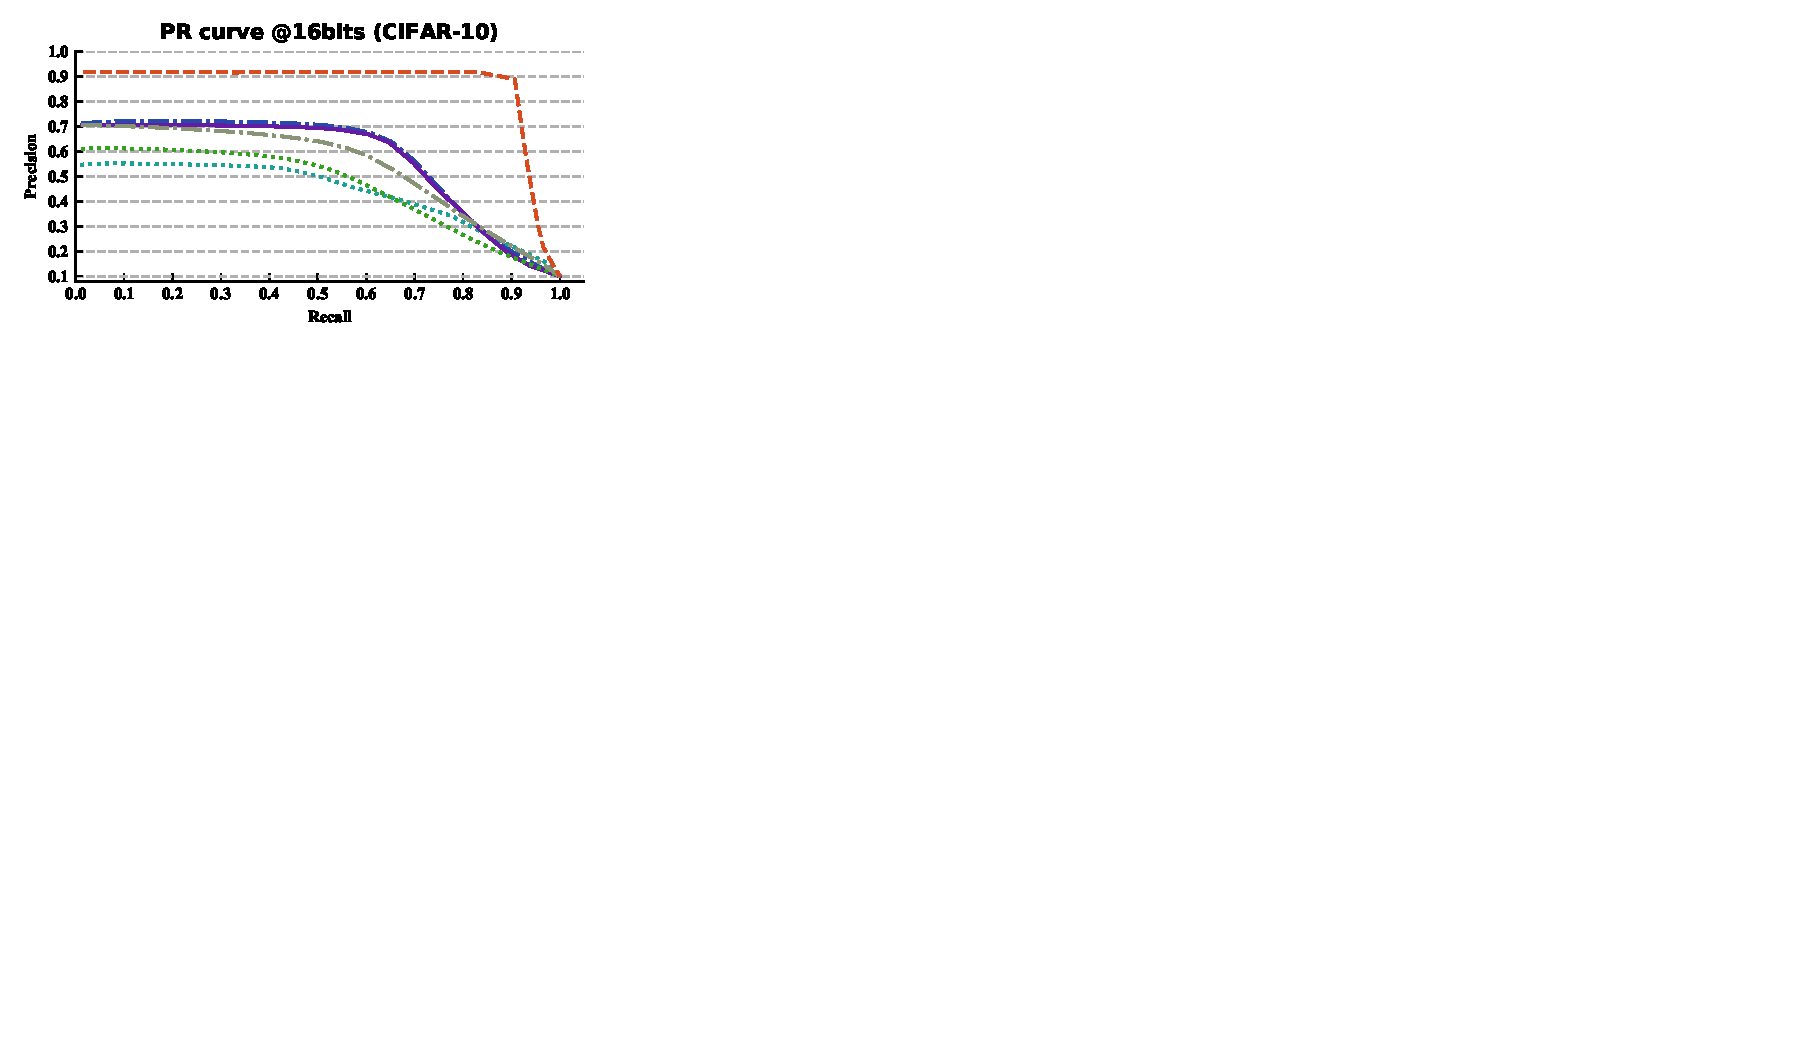
\includegraphics[height=8cm]{04/16prcifar.pdf}
      \caption{16位哈希码下在\textbf{CIFAR-10}上各种方法的\textbf{PR}曲线}
    \end{subfigure}
    \hspace{1cm}
    \begin{subfigure}{\textwidth}
      \centering
      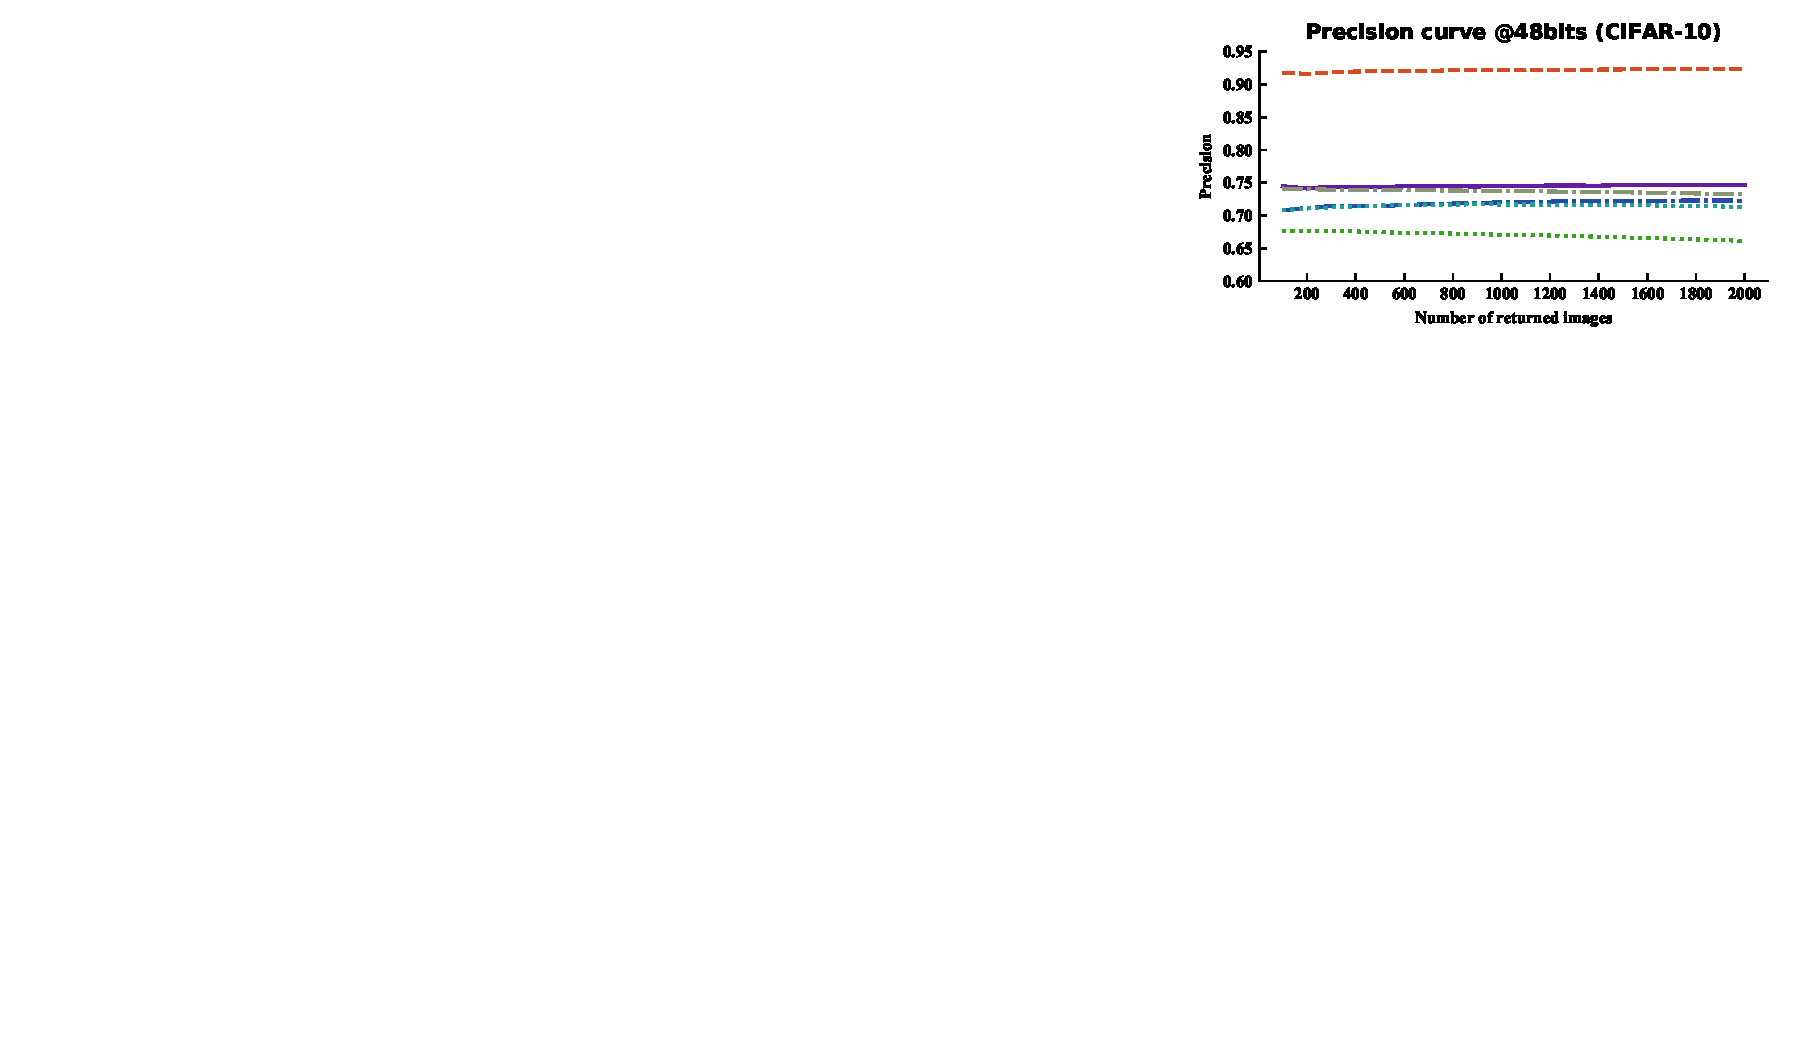
\includegraphics[height=8cm]{04/precifar.pdf}
      \caption{16位哈希码下在\textbf{CIFAR-10}上各种方法的\textbf{Precision}}
    \end{subfigure}
    \bicaption[各种哈希算法在\textbf{CIFAR-10}上的结果]{
        \textbf{TransHash}和其他算法在\textbf{CIFAR-10}数据集上的结果}{The experimental results on \textbf{CIFAR-10}  of \textbf{TransHash} and other competing methods}
    \label{fig:rescifar}
  \end{figure}

  \begin{figure}[!htp]
    \centering
    \begin{subfigure}{\textwidth}
      \centering
      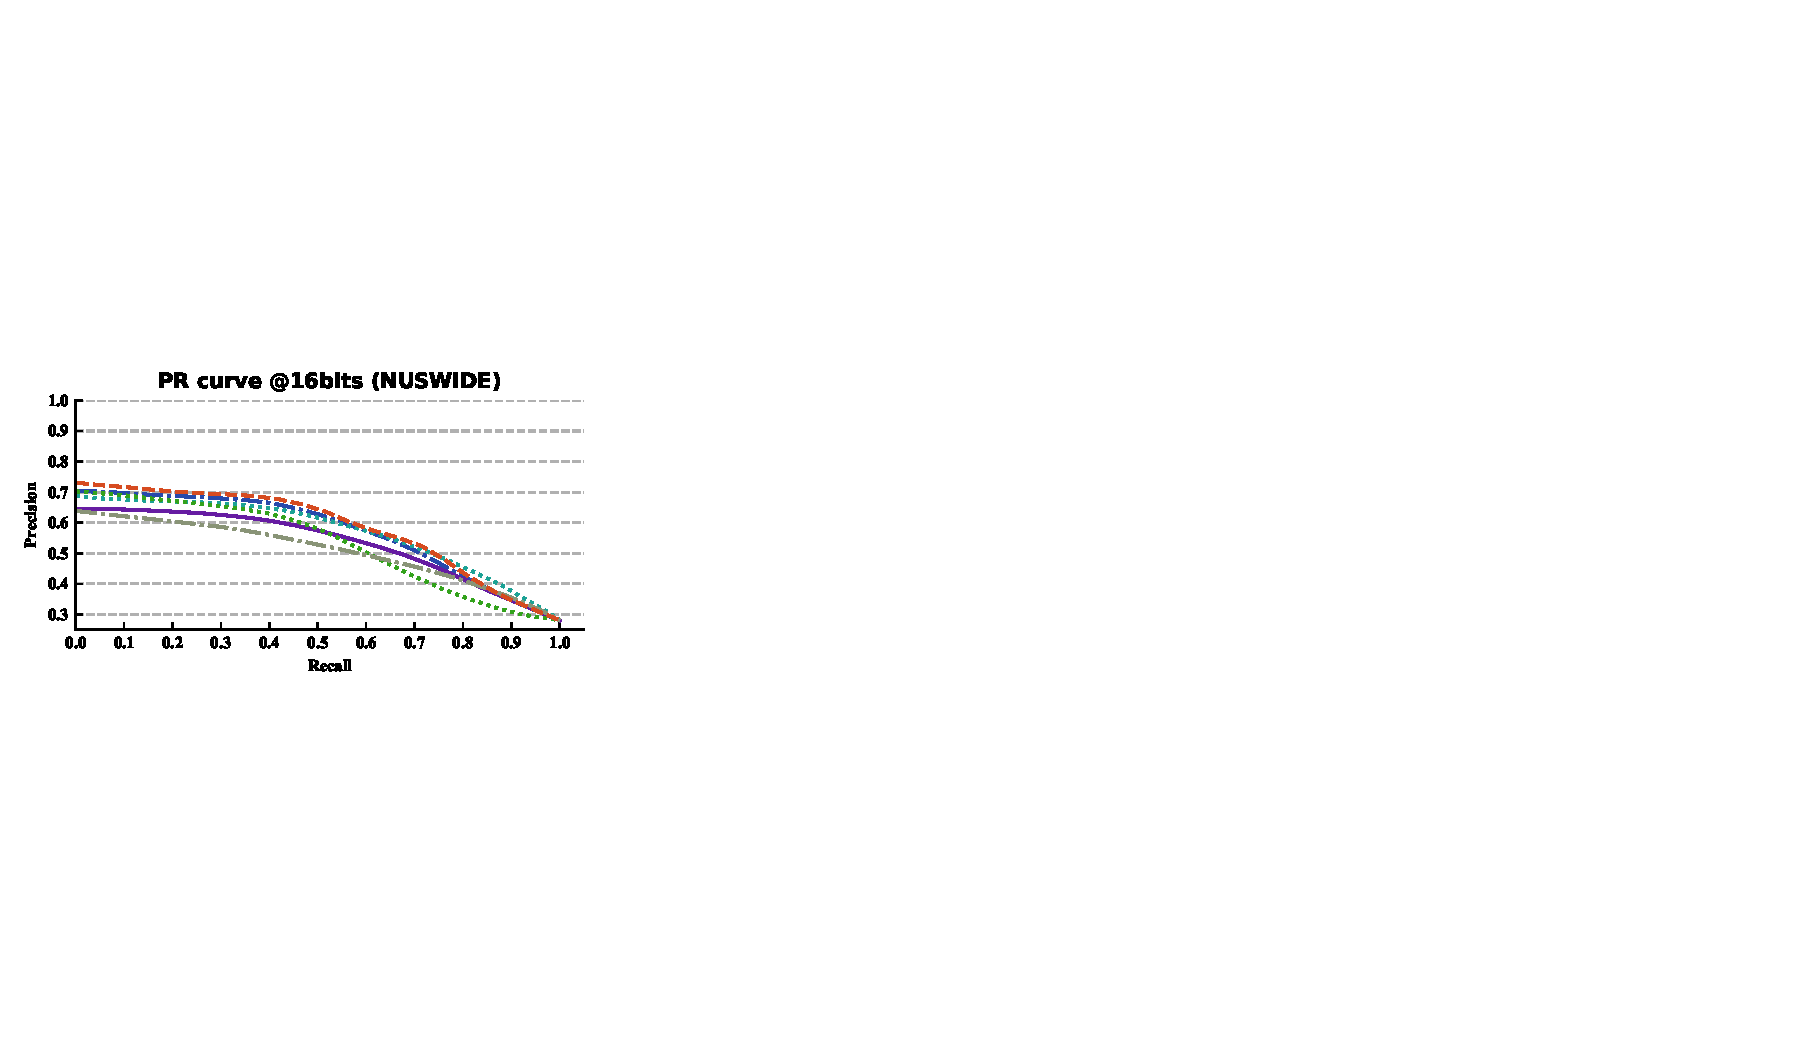
\includegraphics[height=8cm]{04/16prnuswide.pdf}
      \caption{16位哈希码下在\textbf{NUSWIDE}上各种方法的\textbf{PR}曲线}
    \end{subfigure}
    \hspace{1cm}
    \begin{subfigure}{\textwidth}
      \centering
      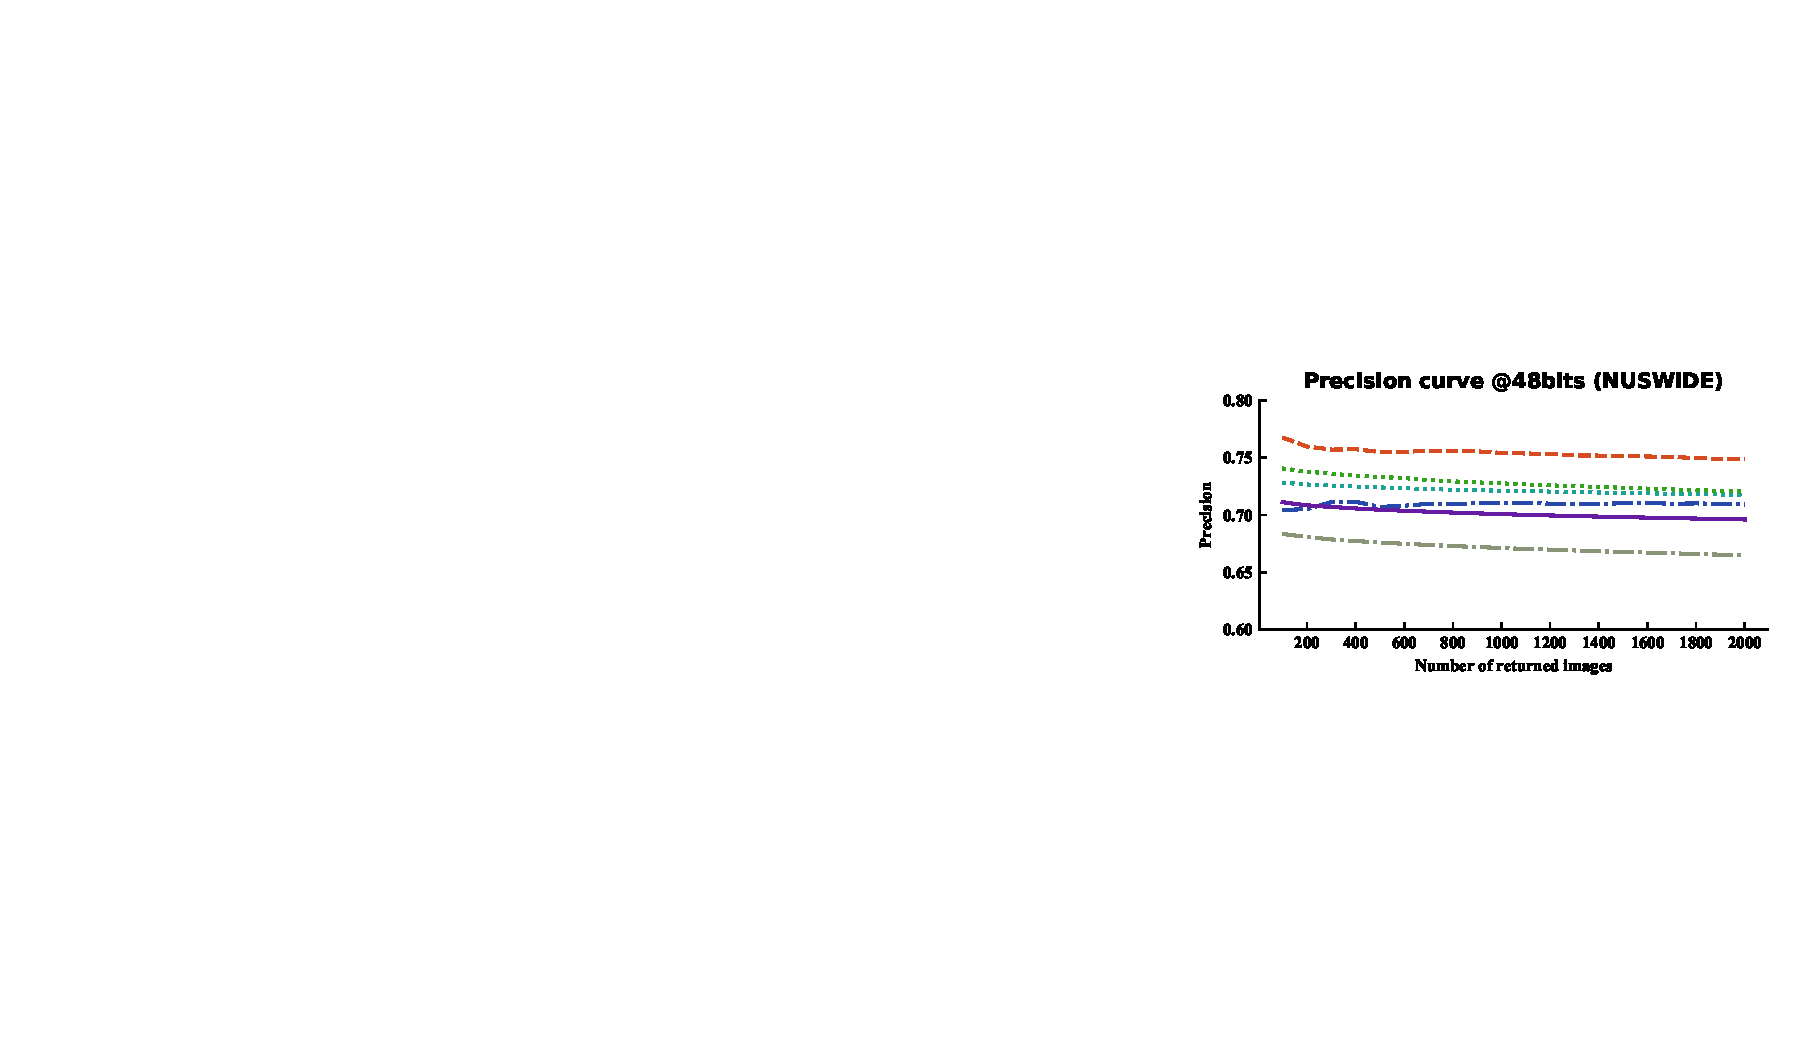
\includegraphics[height=8cm]{04/prenuswide.pdf}
      \caption{16位哈希码下在\textbf{NUSWIDE}上各种方法的\textbf{Precision}}
    \end{subfigure}
    \bicaption[各种哈希算法在\textbf{NUSWIDE}上的结果]{
        \textbf{TransHash}和其他算法在\textbf{NUSWIDE}数据集上的结果}{The experimental results on \textbf{NUSWIDE}  of \textbf{TransHash} and other competing methods}
    \label{fig:nuswide}
  \end{figure}

  \begin{figure}[!htp]
    \centering
    \begin{subfigure}{\textwidth}
      \centering
      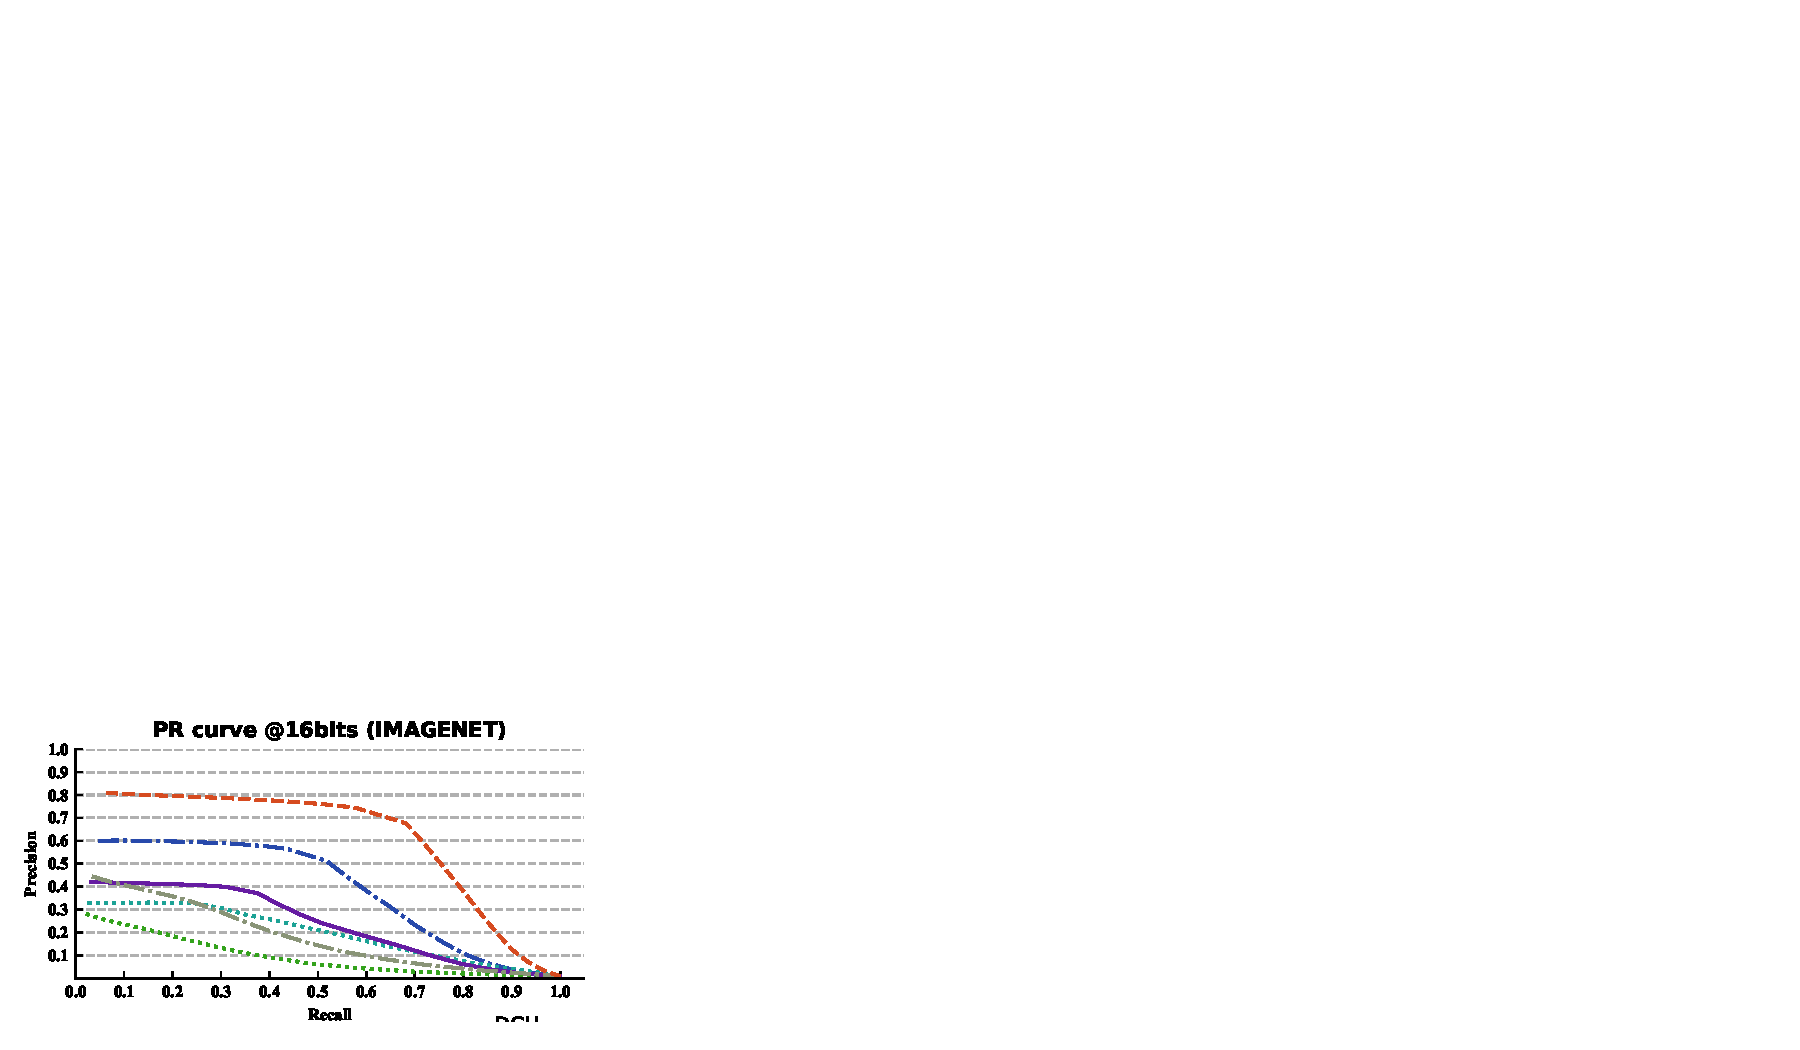
\includegraphics[height=8cm]{04/16primagenet.pdf}
      \caption{16位哈希码下在\textbf{NUSWIDE}上各种方法的\textbf{PR}曲线}
    \end{subfigure}
    \hspace{1cm}
    \begin{subfigure}{\textwidth}
      \centering
      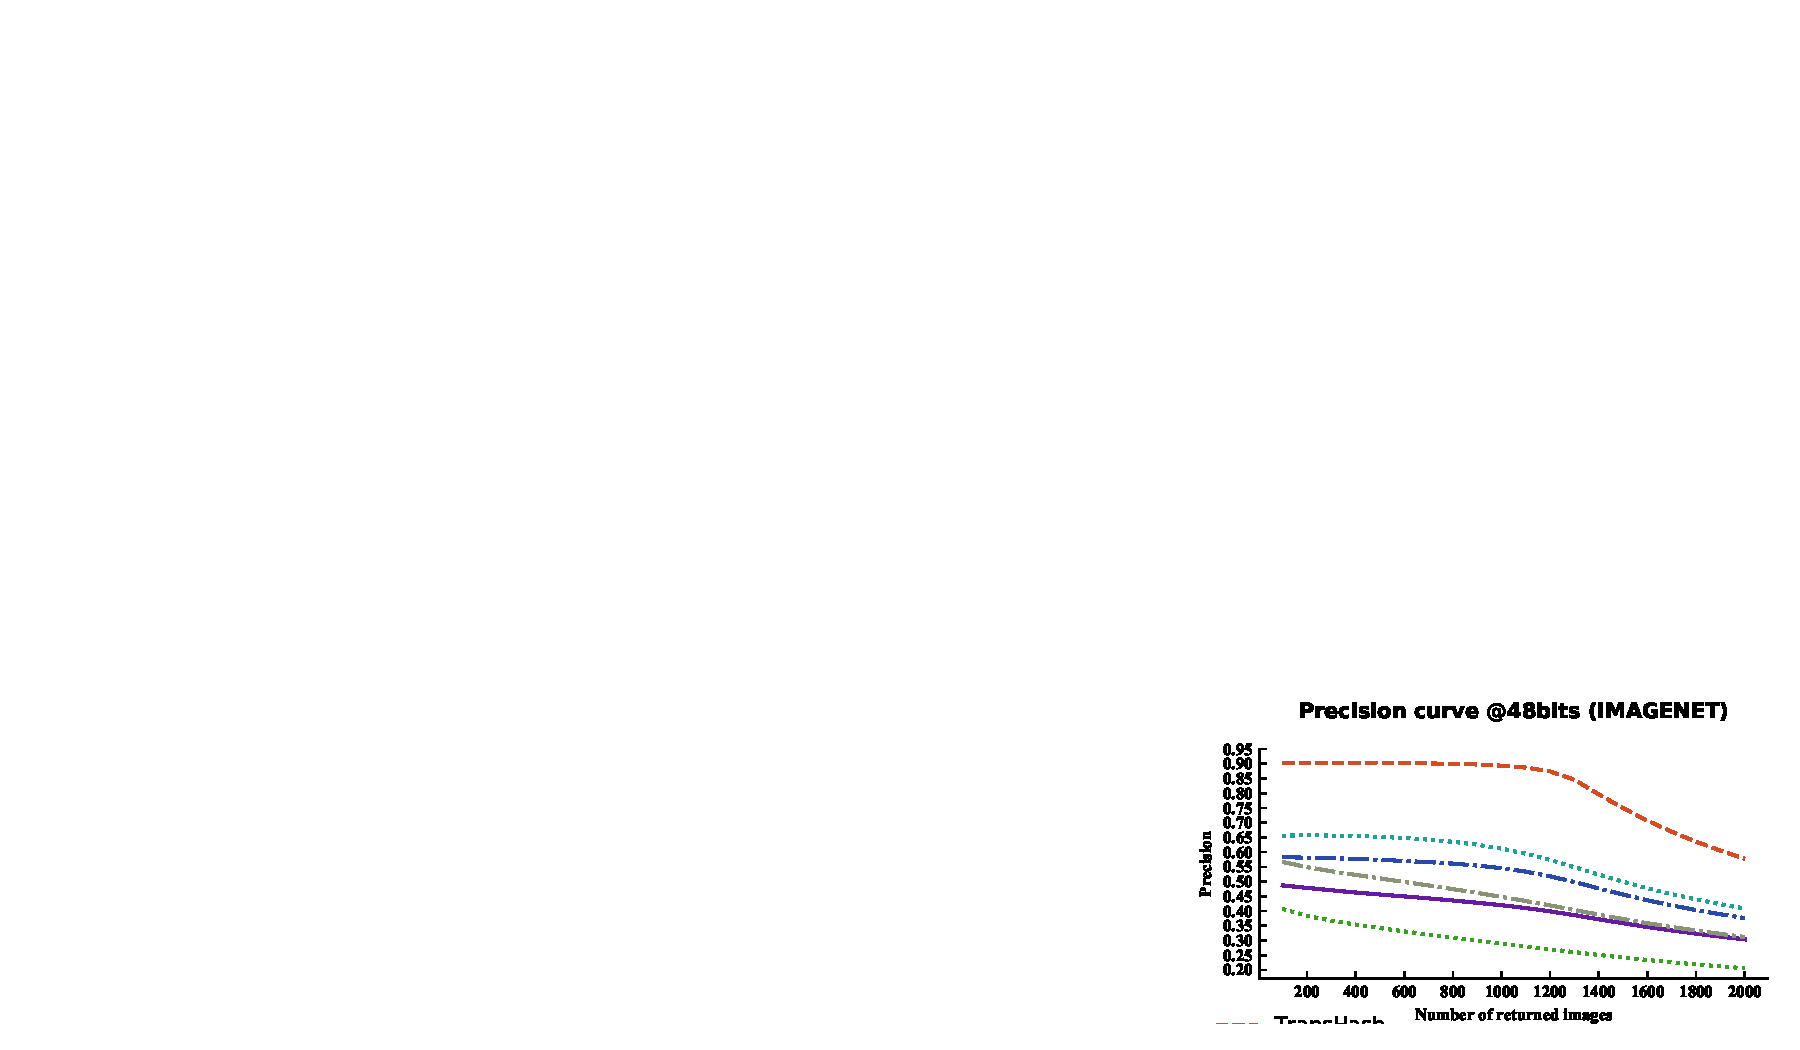
\includegraphics[height=8cm]{04/preimagenet.pdf}
      \caption{16位哈希码下在\textbf{IMAGENET}上各种方法的\textbf{Precision}}
    \end{subfigure}
    \bicaption[各种哈希算法在\textbf{IMAGENET}上的结果]{
        \textbf{TransHash}和其他算法在\textbf{IMAGENET}数据集上的结果}{The experimental results on \textbf{IMAGENET}  of \textbf{TransHash} and other competing methods}
    \label{fig:imagenet}
  \end{figure}
\subsection{与先进方法的对比结果}
在这小节, 我们将本章提出的基于Vision Transformer的架构~\textbf{TransHash}和其他先进的深度哈希算法进行比较。具体来说, 本章进行比较的算法可以被分成两个类别: ``浅哈希方法'' 和``深度哈希方法''。对于``浅哈希方法'', 我们包括了最常见的几个算法\textbf{SH}~\cite{weiss2008spectral},~\textbf{ITQ}~\cite{gong2012iterative},~\textbf{KSH}~\cite{liu2012supervised},~和~\textbf{BRE}~\cite{kulis2009learning}进行细致的比较。对于基于深度学习的哈希方法, 我们包含了第一批基于深度卷积神经网络来解决哈希问题的关注~\textbf{DSH}\cite{liu2016deep12}。同时, 我们还包括了一些最近出现的深度哈希的工作, 例如, ~\textbf{DHN}~\cite{zhu2016deep},~\textbf{HashNet}~\cite{cao2017hashnet},~\textbf{IDHN}~\cite{zhang2019improved} and~\textbf{DPN}~\cite{fan20deep}。 \par
值得注意的是, 对于所有非深度学习的方法和\textbf{DPN}, 我们直接引用Cao~\cite{cao2017hashnet} 和 \cite{fan20deep}的实验结果。对于其他的深度哈希的算法, 我们采用开源的实现代码进行训练并且测试。为了公正的比较, 我们对于算法的超参数和预处理的方法都遵循原先论文中的实验准则。 \par
全类平均精准度(\textbf{mAP})的结果如表~\ref{table:cifar}, 表~\ref{table:nuswide}和表~\ref{table:imagenet}所示。很明显可以看到本章提出的基于Vision Transformer的算法框架在三个数据集上和其他比较的算法而言都能取得非常优异的性能表现。我们的算法在\textbf{NUSWIDE}和\textbf{IMAGENET}上相比较最优的浅层哈希的方法的方法分别取得$19.93\%$,$~39.69\%$的平均\textbf{mAP}提升。在\textbf{NUSWIDE}数据集上, \textbf{ITQ}在 16位, 32位, 48位和64位的哈希长度时取得了 $0.5086$, $0.5425$, $0.5580$, $0.5611$ 的\textbf{mAP} 远低于基于深度哈希的方法。在\textbf{IMAGENET}数据集上, 和深度学习的哈希方法的性能差距更加的显著。基于手工特征的哈希方法的性能不佳的原因主要是因为基于手工描述符的特征难以刻画保留原图片中的具有判别力的特征, 从而导致次优的哈希码。 很明显, 基于深度学习的哈希方法可以取得大幅度的性能提升。\textbf{DPN}算法在\textbf{CIFAR-10}上取得除了本章算法外的最优性能, $0.8305$~\textbf{mAP}。在\textbf{NUSWIDE}上的第二性能由~\textbf{IDHN}取得, $0.7157$ \textbf{mAP}。 在\textbf{IMAGENET}, \textbf{DPN}取得除了\textbf{TransHash}的最优性能, 在4种不同的哈希长度上取得$0.734 $ \textbf{mAP}。\par
很明显, \textbf{TransHash} 依然以大幅度性能提升领先其余基于深度卷积神经网络的算法。\textbf{TransHash}在\textbf{CIFAR-10},~\textbf{NUSWIDE},~\textbf{IMAGENET}上分别取得了$0.9123 $, $0.7419$和 $0.8610$的平均~\textbf{mAP}。具体来说, 在\textbf{CIFAR-10}上, 64位哈希长度时, \textbf{TransHash}取得了$0.9166$的\textbf{mAP}, 比最先进的基于卷积神经网络的方法\textbf{DPN}超出了$8.8 \%$。\textbf{TransHash}在\textbf{IMAGENET}上的性能增长更加显著, 平均\textbf{mAP}超越第二的算法\textbf{DPN}$12.7\%$。 \textbf{TransHash}的性能的增长主要可以归功于两个方面。第一方面是\textbf{TransHash}采取的孪生架构以及双流的特征学习机制可以帮助学习到更加细粒度的特征。


\begin{table}[!htpb]
    %% \centering % not needed
    \bicaption{各个不同的变种在三个数据集上的效果}{Results of different variants on three datasets}
    \centering
    \begin{tabular}{cccccc}
       \\ \hline
    \multicolumn{2}{l|}{Datases} & \multicolumn{4}{c}{\textbf{CIFAR-10}} \\
    \multicolumn{2}{l|}{Methods} & 16-bit & 32-bit & 48-bit & 64-bit   \\\hline
    \hline
    \multicolumn{2}{l|}{\textbf{TransHash}} & 0.9075 & 0.9108 & 0.9141 & 0.9166  \\
    \multicolumn{2}{l|}{\textbf{TransHash w/o C}} & 0.8406 & 0.8384 & 0.8958 & 0.9062  \\
    \multicolumn{2}{l|}{\textbf{TransHash w/o P}} & 0.9029 & 0.9053 & 0.9028 & 0.9014  \\
    \multicolumn{2}{l|}{\textbf{TransHash w/o Q}} & 0.8927 & 0.9023 & 0.9048 & 0.9078  \\
    \hline
    \hline 
    \multicolumn{2}{l|}{Datases} & \multicolumn{4}{c}{\textbf{NUSWIDE}} \\
    \multicolumn{2}{l|}{Methods} & 16-bit & 32-bit & 48-bit & 64-bit   \\\hline
    \hline
    \multicolumn{2}{l|}{\textbf{TransHash}} & 0.7263 & 0.7393 & 0.7532 & 0.7488  \\
    \multicolumn{2}{l|}{\textbf{TransHash w/o C}} & 0.7004 & 0.7265 & 0.7336 & 0.7310  \\
    \multicolumn{2}{l|}{\textbf{TransHash w/o P}} & 0.7190 & 0.7147 & 0.7339 & 0.7167  \\
    \multicolumn{2}{l|}{\textbf{TransHash w/o Q}} & 0.6540 & 0.6821 & 0.6689 & 0.6915  \\
    \hline
    \hline 
    \multicolumn{2}{l|}{Datases} & \multicolumn{4}{c}{\textbf{IMAGENET}} \\
    \multicolumn{2}{l|}{Methods} & 16-bit & 32-bit & 48-bit & 64-bit   \\\hline
    \hline
    \multicolumn{2}{l|}{\textbf{TransHash}} & 0.7852 & 0.8733 & 0.8932 & 0.8921  \\
    \multicolumn{2}{l|}{\textbf{TransHash w/o C}} & 0.7172 & 0.7808 & 0.8064 & 0.8244  \\
    \multicolumn{2}{l|}{\textbf{TransHash w/o P}} & 0.7549 & 0.8485 & 0.8635 & 0.8635  \\
    \multicolumn{2}{l|}{\textbf{TransHash w/o Q}} & 0.7451 & 0.8588 & 0.8689 & 0.8758  \\
    \hline
    \hline 
    \end{tabular}
    \label{table:ablation}
  \end{table}





第二个原因是在\textbf{ImageNet}上相似的图片对和不相似图片对的比例比~\textbf{CIFAR-10}更加严重, 造成了数据不平衡问题, 大大降低了检索的模型性能~\cite{zhang2019improved,liu2016deep12}。\textbf{TransHash}通过动态的对每一个图片对分配一个权重来解决这个问题~ \cite{cao2017hashnet}。在\textbf{NUSWIDE}数据集上, 本章提出的算法也可以在四种哈希长度上均超越所有比较的算法。算法取得的性能提升相比较在其他两个数据集上没有显著的原因主要是因为~\textbf{TransHash}并不是针对多标签检索的场景。\par
我们额外画了基于深度学习的比较模型和\textbf{TransHash}在$16$位哈希码下的\textbf{Precision-Recall}曲线以及在不同的检索返回的图片数量下的\textbf{Precision}曲线。如图~\ref{fig:rescifar}, 图~\ref{fig:nuswide}和图~\ref{fig:imagenet}所示, 对于\textbf{PR}曲线, 代表\textbf{TransHash}的红色曲线始终以大幅度领先其他比较的算法。而对于\textbf{Precision}曲线, \textbf{TransHash}也显著高于所有其他的曲线。在\textbf{NUSWIDE}上, \textbf{TransHash}在\textbf{PR} 曲线上只以微小的优势超过其余方法。对于\textbf{Precision}曲线, \textbf{TransHash}对于检索的返回图片数为$100$时, 得到的精度为$76.77 \%$, 超过\textbf{IDHN}$2.7 \%$。 在\textbf{IMAGENET}, 同样可以观察到非常显著的性能提升。对于$16$位哈希码的\textbf{Precision-Recall}曲线, \textbf{DCH}取得了第二的性能而在$48$时, \textbf{HashNet}则超越了\textbf{DCH}取得了第二的性能。同时很容易观察到\textbf{TransHash}在两种评估指标上都以大幅度领先其余比较的方法。在\textbf{Precision}上, 在检索返回图片数量为$100$和$1000$时候, 我们分别取得$90.35\%$和$ 89.38\%$的精度, 超越\textbf{HashNet} $24.73\%$ 和 $28.18 \%$。这些卓越的性能结果可以充分的证实本章提出的纯粹基于Transformer的深度哈希架构的有效性。
\begin{figure}[!htp]
    \centering
    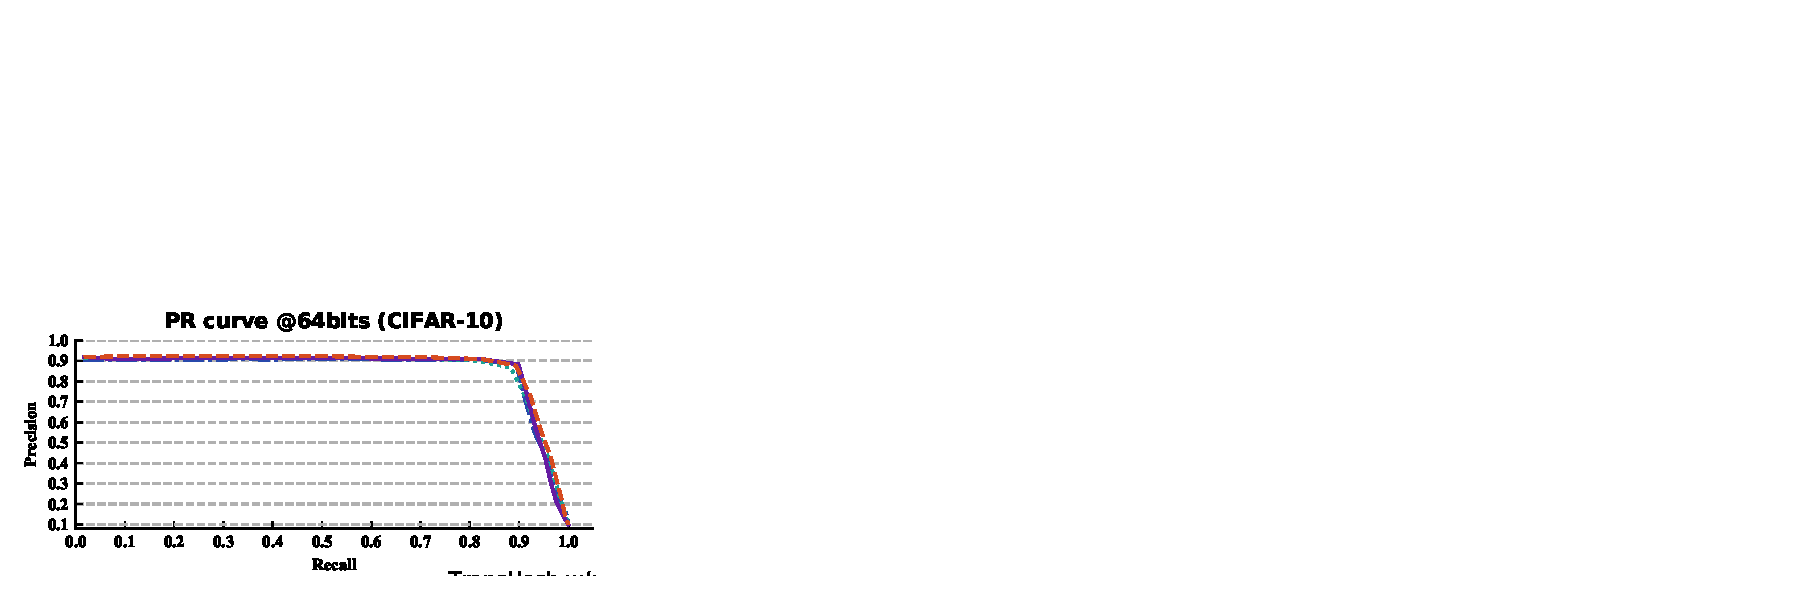
\includegraphics[width=15.5cm]{04/64abcifar10} \\
    \bicaption[在\textbf{CIFAR-10}上的消融实验的结果]
      {不同的变种在$64$位哈希码时的\textbf{CIFAR-10}性能。}
      {The performance of different variants on \textbf{CIFAR-10} of $64$ bits.}
   \label{fig:ablationcifar}
\end{figure}

\begin{figure}[!htp]
    \centering
    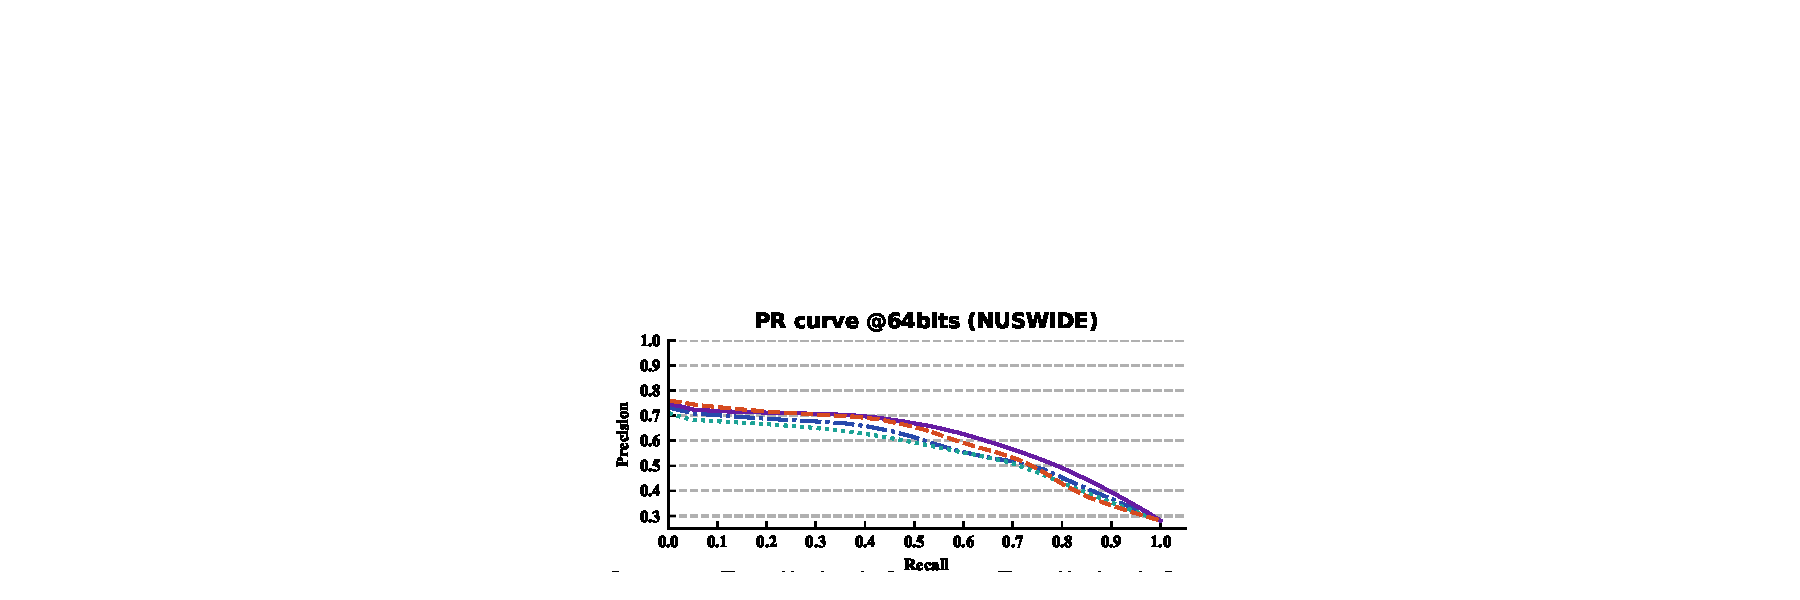
\includegraphics[width=15.5cm]{04/64abnuswide} \\
    \bicaption[在\textbf{NUSWIDE}上的消融实验的结果]
      {不同的变种在$64$位哈希码时的\textbf{NUSWIDE}性能。}
      {The performance of different variants on \textbf{NUSWIDE} of $64$ bits.}
   \label{fig:ablationnuswide}
\end{figure}


\subsection{消融实验}
为了进一步分析本章提出的整个算法框架, 我们进行了一个详细的消融实验来证实框架每一个组成部分的有效性。具体而言, 我们研究了三种基于\textbf{TransHash}的变种:
\begin{enumerate}
    \item \textbf{TransHash w/o P:} 是没有双流特征学习机制的\textbf{TransHash}变种。
    \item \textbf{TransHash w/o Q:} 是没有柯西分布的量化损失函数的变种。
    \item \textbf{TransHash w/o C:} 是继续采取\textit{sigmoid}函数作为生成概率的函数$\sigma(.)$的变种。
\end{enumerate}
如表~\ref{table:ablation} 和 图~\ref{fig:ablationcifar}, 图~\ref{fig:ablationnuswide}以及图~\ref{fig:ablationimagenet}所示, 当没有柯西量化损失函数时, 如\textbf{TransHash w/o Q}所示, 框架经受了明显的性能下降。在\textbf{NUSWIDE}和\textbf{IMAGENET}下, $64$位哈希码的情况下\textbf{mAP}分别从 74.88\% 下降到 69.15\% 以及89.21\% 下降到 87.58 \%。当模型没有采取柯西分布作为概率生成函数时, 如\textbf{TransHash w/o C}所示, 我们可以观察点显著的性能下降。具体来说, 在\textbf{IMAGENET}上, 模型经历了平均$5.55 \%$的\textbf{mAP}下降。我们也注意到在哈希码较短的情况下, 模型的性能损失更加显著。主要的原因是根据Cao~\cite{cao2018deep}, 柯西分布可以有效的拉近相似对的哈希距离至一个较小的范围内, 这使得其在哈希码短的情况下更加的明显。\par

\begin{figure}[!htp]
    \centering
    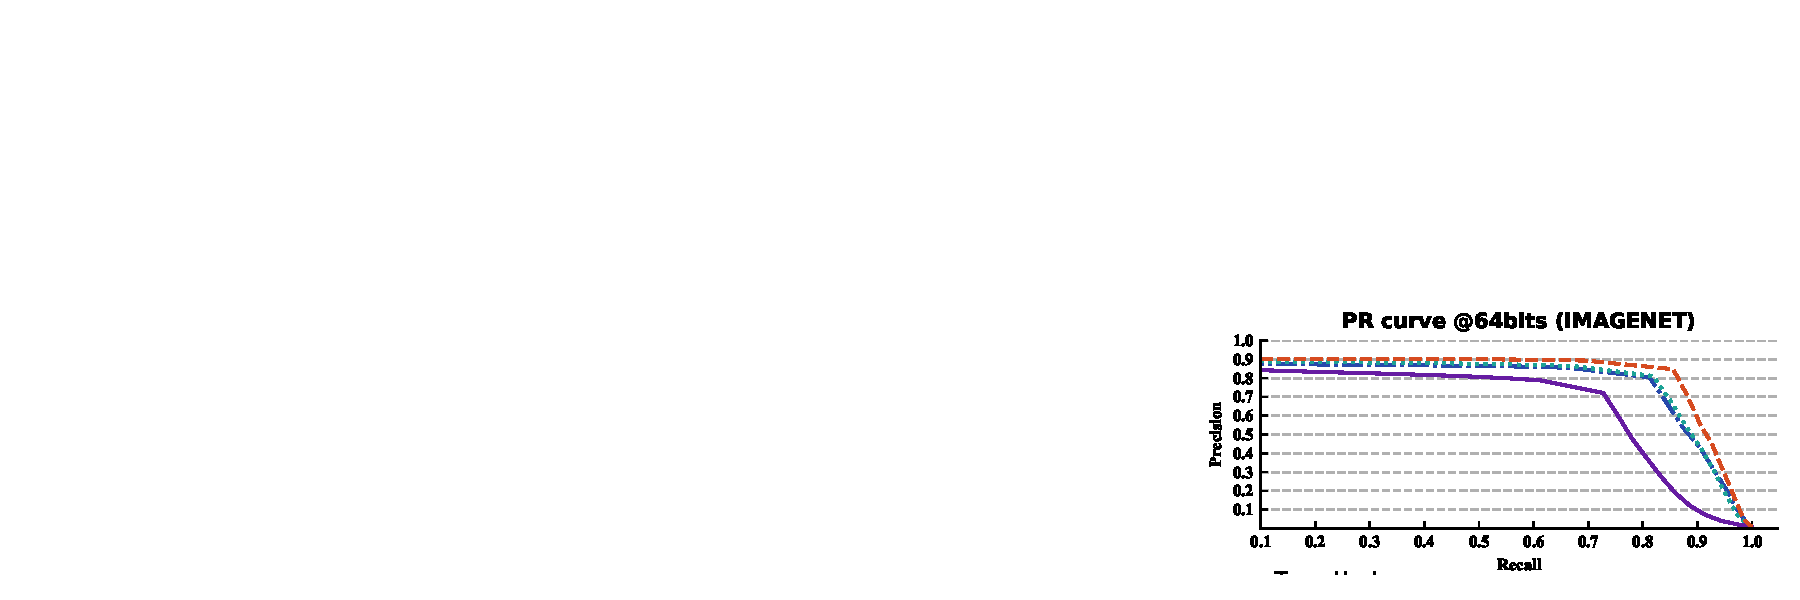
\includegraphics[width=15.5cm]{04/64abimagenet} \\
    \bicaption[在\textbf{IMAGENET}上的消融实验的结果]
      {不同的变种在$64$位哈希码时的\textbf{IMAGENET}性能。}
      {The performance of different variants on \textbf{IMAGENET} of $64$ bits.}
   \label{fig:ablationimagenet}
\end{figure}


最重要的是, 为了测试本章提出的双流特征学习的有效性, 我们也测试了本章提出的孪生模型仅仅包含全局特征学习时时候的性能。如图~\ref{}所示,  \textbf{TransHash w/o P} 的性能持续性的低于具有我们提出的双流特征学习机制的完全模型。在\textbf{NUSWIDE} 和 \textbf{IMAGENET}上, 平均的\textbf{mAP}下降分别是  2.08\% 和 2.83\%。这些实验充足的证明了我们提出的纯基于Transformer的框架的各个组成部分的有效性。\par
由于控制本框架的局部特征的数量的超参数$K$对于模型来说也非常的重要, 我们额外在\textbf{CIFAR-10}进行了详细的实验来对$K$值的敏感性进行探讨。值得注意的是, 如果最终的哈希码的长度是$16$, 并且$K$为2时, 则全局的特征负责生成第一个$8$位的哈希码, 而其余的局部特征每一个负责生成$4$位的哈希码。 \par
如表~\ref{table:ablationk}所示, 通常而言, 模型的性能对$K$的取值并不敏感。同时, 我们也注意到, 当每一个局部特征向量对应生成的哈希码长度少于$4$时候, 模型通常不能收敛。鉴于以上的观察, 我们根据经验将$K$的值设置为$2$。

\begin{table}[!htpb]
    %% \centering % not needed
    \bicaption{$K$值的敏感性分析。`-'指的是模型不能收敛 }{Analysis of the effects of K on CIFAR-10. Note that `-' denotes when K equals a certain number, the model fails
    to converge as illustrated in the empirical analysis.}
    \centering
    \begin{tabular}{ccccccc}
       \\ \hline
    
    \multicolumn{2}{l|}{Groups (K)} & 2 & 3 & 4 & 5  & 66 \\\hline
    \hline
    \multicolumn{2}{l|}{\textbf{16 bits}} & 0.9075 & - & - & - & -  \\
    \multicolumn{2}{l|}{\textbf{32 bits}} & 0.9075 & 0.9013 & - & - & -  \\
    \multicolumn{2}{l|}{\textbf{48 bits}} & 0.9141 & 0.9017 & 0.9187 & 0.9107 & 0.9143 \\
    \multicolumn{2}{l|}{\textbf{64 bits}} & 0.9166 & 0.9103 & 0.9057 & 0.9062 & 0.8994  \\
    \hline 
    \hline
    \end{tabular}
    \label{table:ablationk}
  \end{table}


\section{总结}
在本章中, 我们提出了一个完全基于Transformer的深度哈希框架-\textbf{TransHash}来解决具有挑战性的大规模图像检索的问题。具体来说, 我们提出了一个新型的基于孪生Vision Transformer的架构基于成对的相似度矩阵来提取强健的有判别力的特征。同时, 我们提出设计一个双流特征学习机制来同时学习全局和局部的特征, 从而得到更加细粒度的特征表示。为了进行相似度保留学习, 本章基于一个带权重的贝叶斯学习框架来进行度量学习。本章提出的框架可以通过一个端到端的学习方法进行训练优化。我们在三个标准的大规模图像检索数据集上进行了训练和测试。实验结果表明我们的模型在\textbf{CIFAR-10},~\textbf{NUSWIDE}和~\textbf{IMAGENET}上, 相比较其他先进的基于卷积神经网络的算法可以获得显著的性能提升。
% !TEX root = ../main.tex
\chapter{基于自注意力机制的乘积量化图像检索算法}
在本章中, 我们提出第一个完全基于Vision Transformer的深度乘积量化网络来进行大规模的图像检索-平均精度量化Transformer (Average Precision Quantization Transformer, APQFormer)。\textbf{APQFormer}基于一个双支的Vision Transformer设计了一个深度量化神经网络, 其可以通过同时通过使用不同的图片patch策略学到更具有判别性的特征信息, 又通过一个可以嵌入至深度学习训练中的可导的乘积量化层来进行端到端的量化编码。对于端到端的乘积量化学习, 现在的算法大多数使用基于排序的量化损失函数, 而这样的方法并不能保证优化最终的评价指标-平均精度均值(Mean Average Precision, mAP)。我们提出了一个新型的量化损失函数-平均精度量化损失(Average Precision Quantization Loss, APQ loss)。其通过对查询的数据使用原向量而被检索的图片使用量化后的特征向量来将量化编码检索时的非对称检索特性嵌入至度量学习设计中。同时, 其通过直接优化训练过程中每个批次数据计算得到的平均精度(Average Precision, AP)来同时学习保留了相似度的特征向量以及紧凑的乘积量化编码。本章在两个标准的大规模检索数据集-\textbf{CIFAR-10}和\textbf{IMAGENET}-上进行了广泛的实验。实验结果正式了\textbf{APQ}与先进算法相比具有更加优越的性能, 从而证实了算法设计的有效性。
\section{引言}
现代社会中每日的多媒体数据量以爆炸性的速度增长, 这导致了针对大规模检索的近似最近邻搜索技术的迅速发展于成熟~\cite{andoni2006near,shrivastava2014densifying, malkov2018efficient, nie2020deep, li2021dahp}。在近似最近邻技术中, 深度哈希算法由于其检索的速度以及较低的存储开销成为了主流被采用的方法~\cite{zhu2016deep, jiang2018asymmetric, zhang2019improved, cao2017hashnet}。具体来说, 在基于深度学习的大规模图像检索中, 每一张图片是由一个紧凑的哈希码来表示, 并且通过哈希码进行图片间的迅速的距离计算~\cite{jang2020generalized}。\par
通常来说, 深度哈希方法可以被分为两种: 深度汉明哈希 (Deep Hamming h、Hash, DHH) 和深度乘积量化(Deep Product Quantization, DPQ)。基于深度汉明哈希的方法通常通过学习一个哈希函数来将在原始像素图片映射到汉明空间并且图片对应的二进制汉明哈希码需要保留原始图片的视觉相似性~\cite{zhu2016deep,zhang2019improved, cao2017hashnet, cao2018deep, fan2020deep}。基于学习二进制汉明哈希码的哈希方法其中一个优势是, 由于汉明距离的计算可以通过\textbf{XOR}的位操作来进行加速计算, 检索速度可以大大的提高。但是其也有一个主要的缺点, 汉明距离的区分度有限, 会导致损失一大部分原特征向量的有判别性的特征。基于深度乘积量化的方法, 一种使用乘积量化来对深度神经网络生成的特征向量进行压缩编码的检索方法, 因此获得了学术界和工业界的广泛关注。\par

\begin{figure}[!htp]
  \centering
  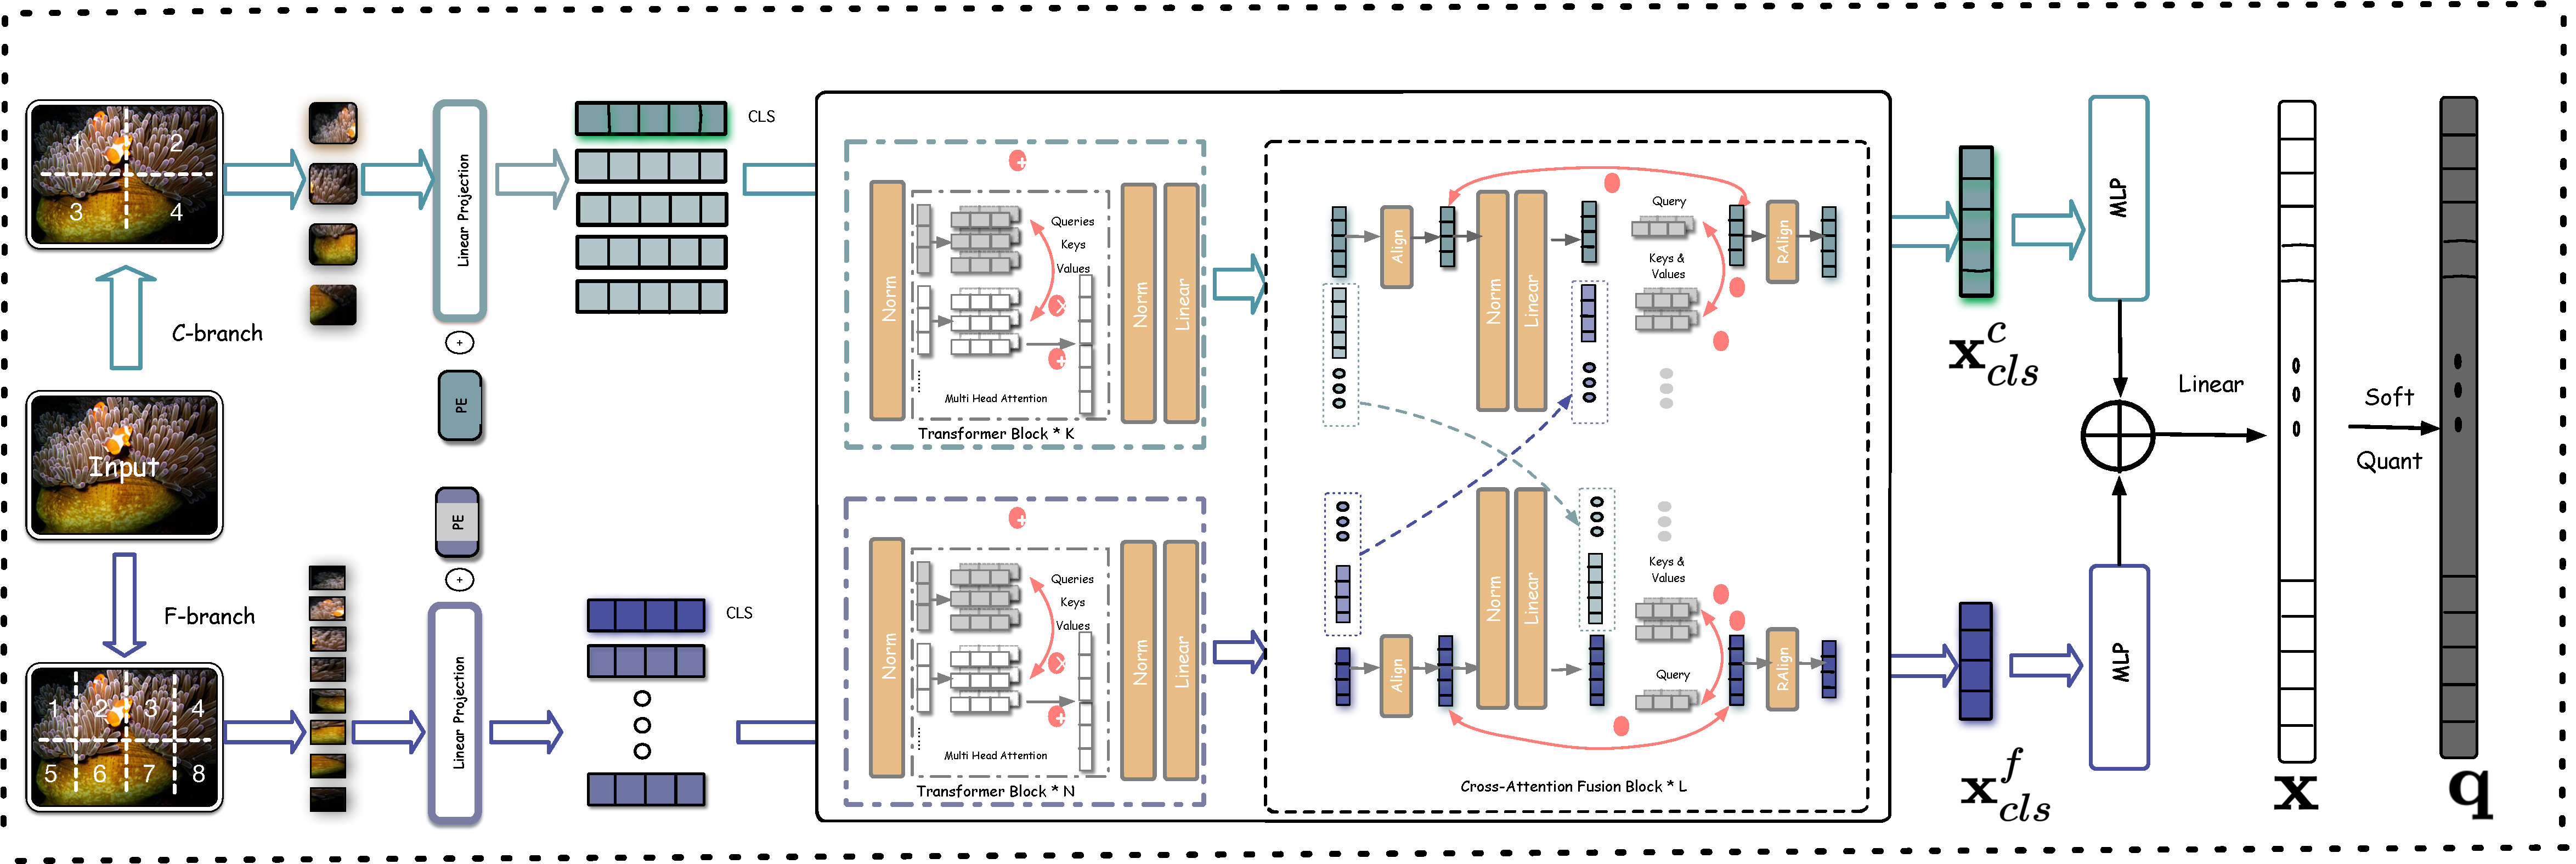
\includegraphics[width=15cm]{05/main1.pdf} \\
  \bicaption[基于Vision Transformer的深度乘积量化框架]
    {基于Vision Transformer的深度乘积量化框架~\textbf{APQFormer}。框架的左边是基于双支的Vision Transformer架构用于多尺度细粒度特征提取。右边包含一个软乘积量化层用于进行乘积量化学习。}
    {The detailed architecture of the proposed \textbf{APQFormer} for deep product quantization learning. The left part of the figure illustrates the dual-branch vision transfomer-based network for fine-grained feature learning. The right part exibits the soft  quantiation layer for product quantization learning. }
 \label{fig:mainapq}
\end{figure} 


乘积量化(Product Quantization, PQ)将原有的特征空间分解成$\mathbf{M}$个子空间。随后, 每一个子空间被量化成$\mathbf{K}$个组(sub-codewords)~\cite{klein2019end}, 这样总共生成了$\mathbf{M}$本 sub-codebook以及$\mathbf{M}\times\mathbf{K}$个sub-codewords。 对于一个输入向量$\mathbf{x} \in  \mathbb{R}^{MD}$, 它先被分割成$\mathbf{M}$个属于 $\mathbb{R}^D$空间的子向量, $ \mathbf{x} =  [\mathbf{x}_1,\mathbf{x}_2,...,\mathbf{x}_M]$。随后, 它通过对每个子向量进行向量量化编码得到一个紧凑的哈希码 $z_x \in \{0,1\}^{M. \log_2{K}}$。这个哈希码是由$\mathbf{M}$组$\log_2{K}$位的短哈希码拼接而成。对于第$m$个$\log_2{K}$的短哈希码, 它代表着输入的第$m$个子向量对应的sub-codeword在第$m$本sub-codebook中的索引,  $i \in \{0,\cdots,K-1\}$。\par
基于深度乘积量化的检索方法通常包含两个阶段: (1) 基于深度卷积神经网络,例如AlexNet,的特征学习。(2)基于上一阶段学习到的特征向量的乘积量化学习。以往的先驱算法通常采取一个二阶段的学习方法~\cite{yue2016deep, liu2018deep, cao2017deep}。第一阶段一般通过监督学习的方法来学习生成有判别性的特征向量。在第二阶段, 通常使用无监督的K-means聚类方法来学习每个sub-codebook中的所有sub-codewords。 尽管这些方法取得了一定程度上的成功, 基于无监督的量化在乘积量化生成codewords的阶段忽略了监督信号的作用, 从而只能达到次优的性能。 \par
\begin{figure}[!htp]
  \centering
  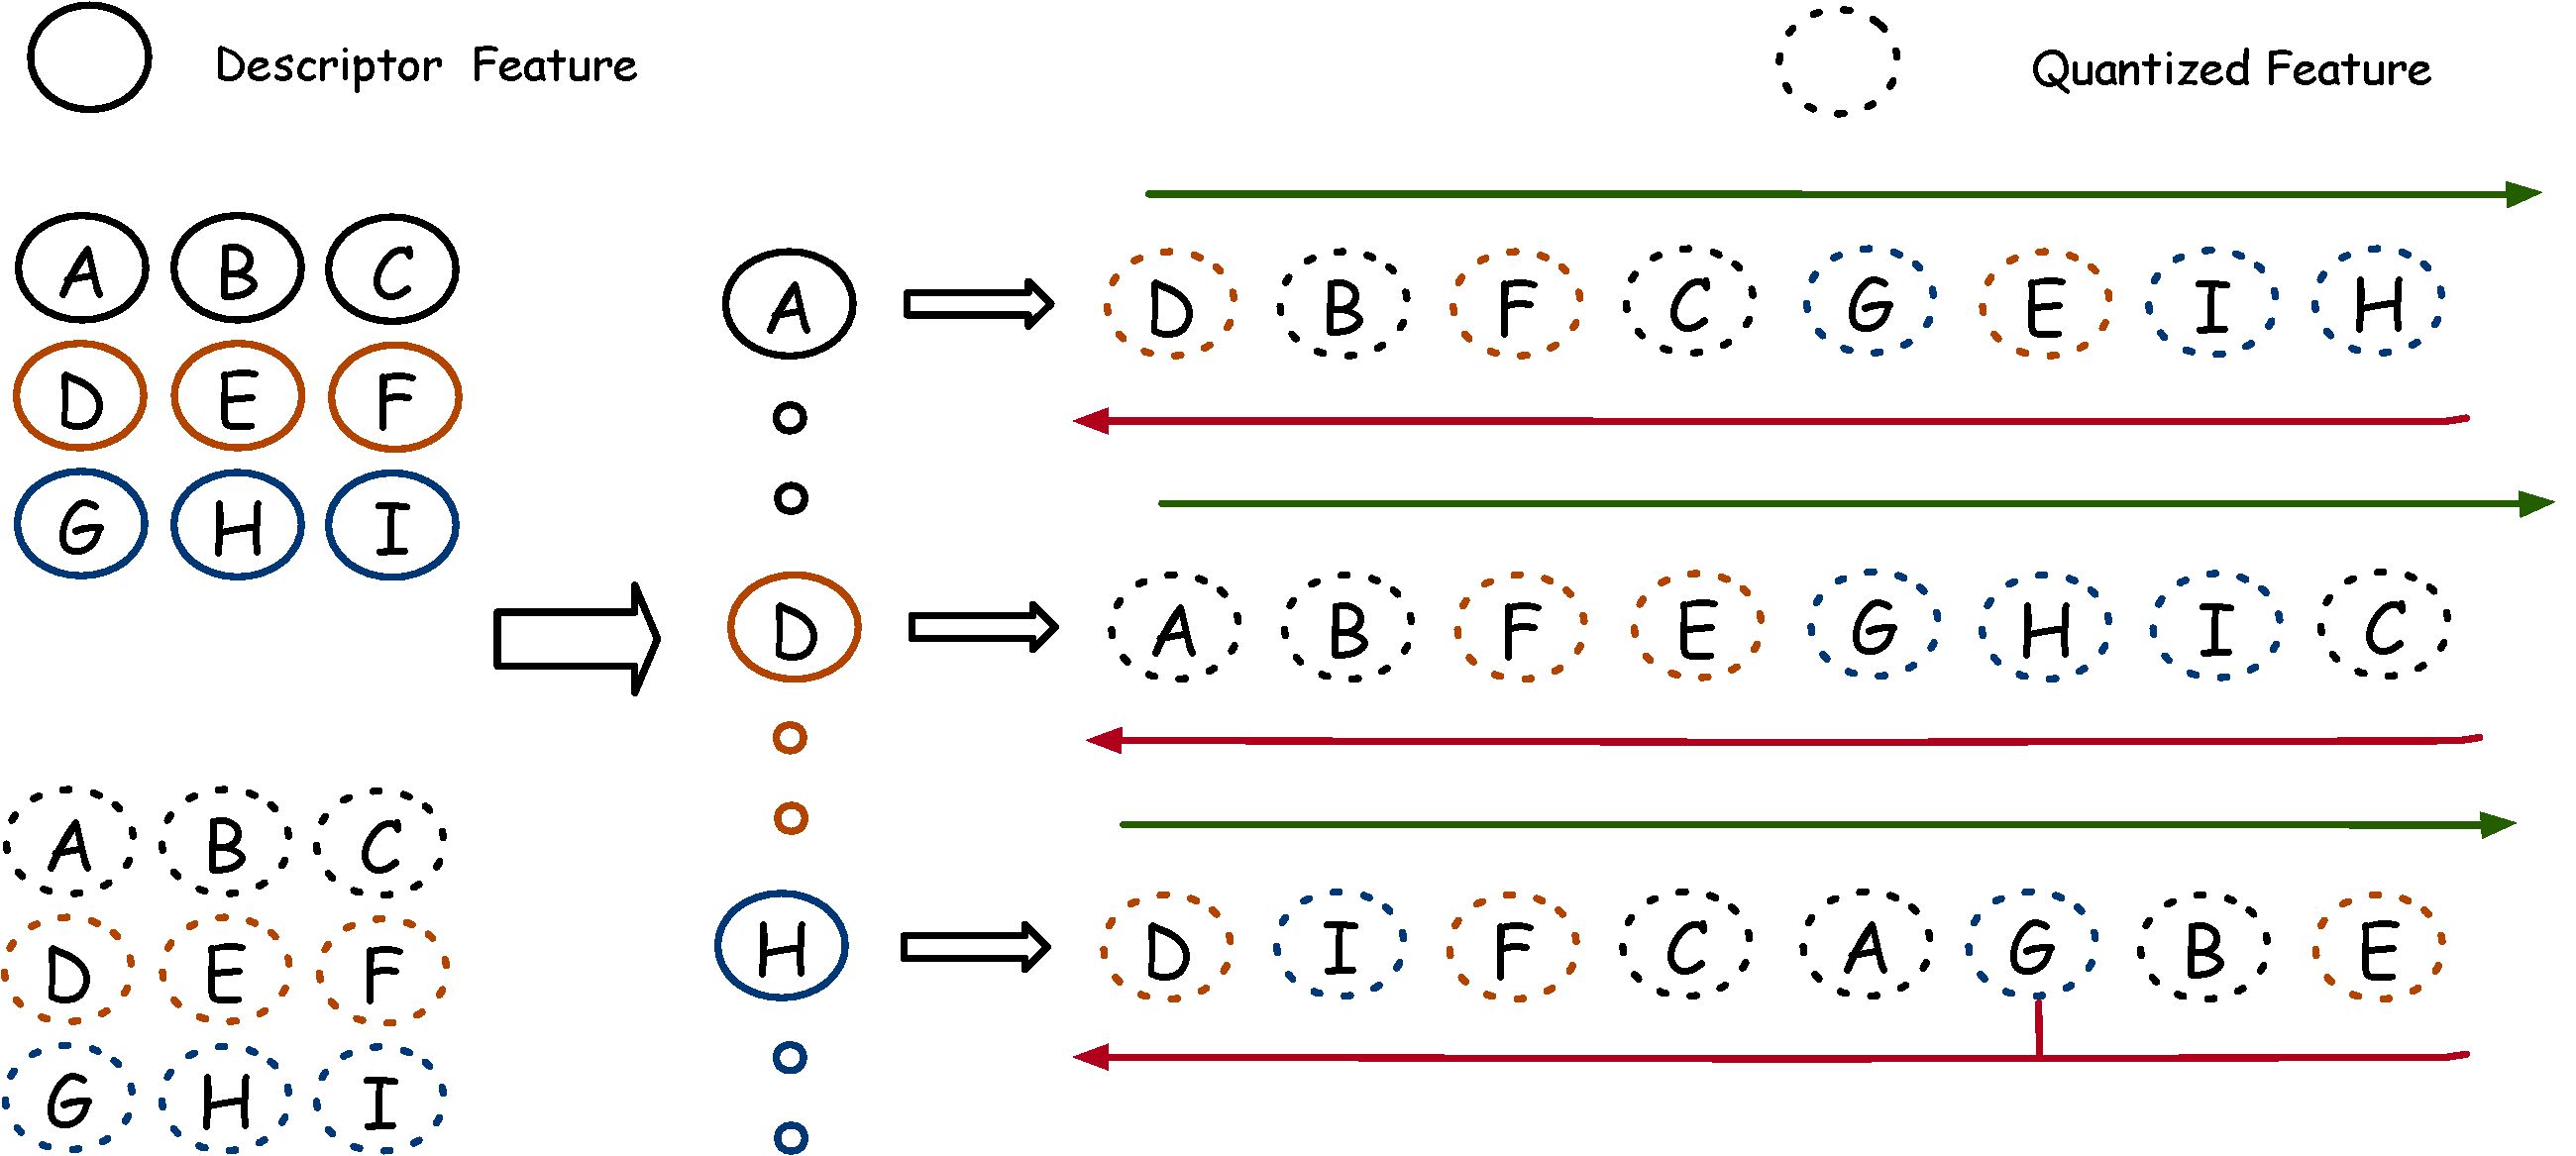
\includegraphics[width=15cm]{05/main2.pdf} \\
  \bicaption[直接优化平均精度\textbf{AP}的量化损失函数]
    {平均精度量化损失函数-\textbf{APQ}的描述。}
    { The description of the average product quantization (\textbf{APQ}) loss.}
 \label{fig:mainapq1}
\end{figure} 

我们通过合并以上两个阶段, 将乘积量化融入到监督学习框架中从而端到端的进行乘积量化学习。受以往工作~\cite{jang2020generalized, yu2018product, dosovitskiy2020image, chen2021crossvit}等的启发, 我们提出一个基于双支Vision Transformer的乘积量化神经网络如图~\ref{fig:mainapq}所示。 其通过两个不同的分支对不同的图片大小分块学习融合的多粒度特征, 同时通过一个可以训练的乘积量化层来对特征向量进行量化。对于相似度保持的量化学习, 迄今为止有不少基于排序损失设计的量化损失函数, 例如基于三元组的损失函数~\cite{jegou2010product}以及n元组的损失函数~\cite{jang2020generalized}。然而, 如Revaud所示~\cite{revaud2019learning}, 优化基于排序损失的目标函数并不能保证优化我们的最终评估指标~\textbf{mAP}。同时, 这些量化损失函数需要机器学习从业人员手工对高敏感的超参数进行微调, 例如三元损失函数中的边界超参数~\cite{cakir2019deep}。为了解决以上的问题, 我们设计了一个新型的量化损失函数-平均精度量化损失(\textbf{APQ})-来进行相似度保持的端到端的监督乘积量化学习, 如图~\ref{fig:mainapq1}。平均精度(Average Precision, AP)的计算是不可导的, 非常难通过传统的基于梯度的框架进行优化。我们通过histogram binning 的方法重新定义\textbf{AP}的计算, 同时采取线性插值的方法来将不可导的直方图桶计数的问题转化成为一个可导的连续性的目标函数。具体来说, \textbf{APQ}通过将未量化的特征向量当作查询向量, 量化后的向量当作被检索的向量。在得到一个返回的检索向量排序集后, 通过在这个返回的列表计算一个\textbf{AP}的可梯度优化的替代目标来进行优化。通过这个\textbf{APQ}新型的度量学习目标函数, 本章提出的框架可以直接可以直接学习到紧凑的乘积量化编码并且这种编码在评估指标\textbf{mAP}上是最优的。 总而言之, 本章的主要工作与贡献如下:
\begin{enumerate}
    \item 本章设计了第一个完全基于Transformer的深度乘积量化框架来进行大规模的图像检索-\textbf{APQFormer}。其包含了一个新型的双支Vision Transformer的乘积量化网络来进行端到端的多尺度特征学习以及一个新型的量化损失函数用于监督进行相似度保留学习。
    \item 本章提出了一个新型的量化损失函数, 平均精度均值量化损失(\textbf{APQ})来进行语意保留的度量学习。它直接在检索返回的量化后的特征向量列表上优化平均精度(\textbf{AP})的连续的可导的替代目标函数。通过最小化这个损失函数, 我们可以直接优化在测试阶段使用乘积量化使用非对称的检索策略进行检索时候的评估指标(\textbf{mAP} )。
    \item 本章在两个标准的公共大规模检索数据集上进行了不同哈希长度下的检索实验-\textbf{CIFAR-10}和\textbf{IMAGENET}。实验结果表明本章提出的框架-\textbf{APQFormer}-可以取得比先进算法显著的性能提升, 证实了算法的有效性。
\end{enumerate}

\section{相关工作}
早期的针对高效的图像检索工作依赖于手工提取的特征 (例如, SIFT~\cite{lowe2004distinctive}) 来得到刻画图片的特征用于后续的哈希码的生成。这种方法一般被称作是浅哈希方法。典型的工作包括无监督的浅层哈希方法 (\textbf{SH}~\cite{weiss2008spectral}, \textbf{ITQ}~\cite{gong2012iterative} 和\textbf{MLH}~\cite{norouzi2011minimal}) 和有监督的浅层哈希方法 (\textbf{KSH}~\cite{liu2012supervised} 和 \textbf{BRE}~\cite{kulis2009learning})。确切地说, \textbf{SH}~\cite{weiss2008spectral}提出最小化图片对之间的带权的汉明距离。同时, \textbf{ITQ} 通过基于在手工提取的特征上最小化量化误差来最小化将实值特征向量二值化的信息损失。为了使用监督标签来获得更好的语义保留的效果,~\textbf{KSH}~\cite{liu2012supervised}和\textbf{BRE}~\cite{kulis2009learning}提出在核空间进行相似度语义保留的哈希学习。尽管这些方法取得了一定程度上的成功, 但是由于手工提取的特征很难准确的保留图像中的语义信息, 这些方法只能取得次优的性能。\par
靠虑到于这一个主要的限制点, 利用卷积神经网络(例如, AlexNet~\cite{alexnet}, ResNet~\cite{he2016deep})来进行端到端的特征提取的深度哈希算法开始获得科研人员的大量关注。它们一般可以被分为两个类别: (1)深度汉明码哈希方法 和深度乘积量化的方法。深度汉明哈希的方法通过深度神经网络学习到一个哈希函数将图片从原本的空间映射到一个汉明空间, 并且在汉明空间中保持原图片的相似性。典型的例子包括\textcircled{1}单点哈希方法~\cite{lin2015deep}, \textcircled{2}成对哈希方法~\cite{liu2016deep,cao2017hashnet,cao2018deep,fan2020deep} \textcircled{3} 三元组哈希方法~\cite{lai2015simultaneous,wang2016deep,li2019triplet}。\textcircled{1}单点哈希方法主要包含: Lin~\cite{lin2015deep}是第一批探究深度卷积神经网络在哈希学习中的工作。通过使用在ImageNet上预训练的AlexNet模型在哈希的数据集上进行分类微调, 然后采取分层次的方法进行检索。\textcircled{2}成对的哈希方法主要有: Liu 和 Cao等人\cite{liu2016deep,cao2017hashnet}提出基于一个贝叶斯学习的框架基于成对的图片输入以及其对应的图片对之间的相似度标签来进行度量学习, 以及对应的量化损失函数来降低连续性的哈希向量和二进制哈希码之间的信息差。Cao~\cite{cao2018deep}提出了一个基于柯西分布作为概率输出函数, 使用成对的交叉熵损失进行度量学习来学习紧凑的哈希编码。 \textcircled{3}三元组的哈希方法通常是使用三元损失函数进行相似度保留的度量学习。2015年, Lai等人~\cite{lai2015simultaneous}提出第一个基于三元损失函数的排序损失进行哈希学习, 并且通过一个divide-and-conquer的模块生成哈希码并且降低哈希码的冗余。然而以上基于排序损失改进的哈希算法都是在优化essential loss~\cite{liu2011learning}, 这是平均精度均值\textbf{mAP} 的一个上界。因此, 优化这些目标函数不一定能够保证可以优化最终的评估指标\textbf{mAP}。 为了解决这个问题, He等人~\cite{he2018hashing}提出一个tie-aware的哈希框架将汉明距离的整数性质考虑进其中, 同时通过直接优化\textbf{mAP}以及归一化折损累积收益~\textbf{NDCC}来进行端到端的哈希训练。\par
由于二进制哈希码的生成一般需要使用一个不能导的\textit{Sign}激活函数来进行量化导致无法端到端通过梯度下降的方法进行训练, 现阶段的``深度汉明哈希方法''通常采取持续放松~\cite{liu2016deep}的方法来绕过这一难题。它们采取的做法是通过在训练阶段优化一个放松的连续的可导的目标函数, 然后在测试阶段使用\textit{Sign}函数进行二值化生成二进制的编码。然而由于放松后的连续性的目标函数已经远离了原始的离散优化的目标函数, 这通常会导致次优的性能。``深度乘积量化''方法通过使用乘积量化将原始的连续性高维向量量化成二进制编码可以有效的解决上述的问题。\textbf{DQN}\cite{yue2016deep}是第一个探究乘积量化~\cite{jegou2010product,ge2013optimized,zhang2014composite}在深度哈希上应用的工作。它采取了一个成对的训练策略基于余弦损失函数来学习实值的特征向量以及一个随后的量化损失函数来进行无监督的乘积量化学习。 Liu等人随后提出了一个三元量化方法~ \cite{liu2018deep}, 通过提出一个组内最难三元组生成方法动态在每个批次的输入组建困难的三元组, 然后使用三元损失函数进行度量学习。然而这样的方法有一个关键的缺陷, 从而导致了性能的下降。由于基于这种机制的乘积量化的过程和深度神经的监督训练过程分离开来, 并且是基于无监督的k-means聚类算法来实现。由于基于k-means的聚类的乘积量化过程无法使用监督的标签进行训练, 也无法反馈调整前一阶段的特征学习的效果, 这种模式的性能大大的受限。因此, Yu, Klein 以及Jang等人~\cite{yu2018product, klein2019end,jang2020generalized}提出将乘积量化融合进入端到端的深度神经网络监督训练中, 通过\textit{Softmax}来在训练阶段接近乘积量化的效果。\par
Transformer最初是由\textbf{Google}公司提出在自然语言处理替代基于编码器和解码器的神经网络架构~\cite{vaswani2017attention}。一经提出, \textbf{Transformer}就迅速成为了自然语言处理领域的标准主干神经网络框架。2020年末, \textbf{Google} 又进一步提出Vision Transformer (ViT) 将Transformer引入到计算机视觉领域, 从而成为了卷积神经网络的一个极强的替代神经网络模型。从此, 基于Vision Transformer的计算机视觉模型开始迅速发展, 在各个计算机视觉任务上展现出比卷积神经网络更优越的性能。DeiT~\cite{touvron2021training}~是一个Transformer可以在中等大小的数据集上进行预训练并且取得较有的性能。DeiT通过使用CNN的输出当做一个教师模型, 通过蒸馏学习(Distillation Learning)来帮助训练自身的Transformer架构。在输入的嵌入表征前, 它们添加了一个蒸馏表征, 然后通过交叉熵损失和蒸馏损失进行训练。随后 Token-to-Token (T2T) Vision Transformer~\cite{yuan2021tokens}递归的将临近的token融合成一个token来降低序列的长度并且对于空间中的较远的联系进行建模。 Liu等人\cite{liu2021swin} 提出了Swin Transformer, 一个基于Vision Transformer的变种。其通过提出Window Self Attention 将自注意力的计算限制在固定大小的窗口内从而极大的降低计算复杂度, 使得Vision Transformer可以处理更大的现实视觉任务。 He 等人\cite{he2021transreid}提出了第一个完全基于Transformer的行人重识别框架, 并且在多个行人重识别以及车辆重识别领域获得了超越当前最先进的基于卷积神经网络的重识别框架的性能。Wang等人 \cite{wang2021pyramid}提出一个Pyramid Transformer来进行密集预测。 Cheng等人\cite{wang2021crossformer}提出了一个跨尺度的Transformer来学习更加细粒度的图像特征来进行图像分类任务。 随后, Chen~\cite{chen2021regionvit}提出一个新型的 region-to-local 注意力机制来替代原ViT中的自注意力机制。为了学习到更多的细粒度特征, Chen\cite{chen2021crossvit} 设计了一个双支的Transformer框架来学习图像中不同尺度的特征。\par
在本章中, 受以往的工作的启发 \cite{chen2021crossvit,cakir2019deep,revaud2019learning}, 我们提出了一个平均精度均值量化Transformer (Avereage Precision Quantization Transformer, \textbf{APQFormer})。具体来说, 受Chen和Yu的工作启发\cite{chen2021crossvit,yu2018product}我们设计了一个双支 Vision Transformer 量化神经网络来进行端到端的特征学习。对于相似度保留的度量学习, 本章采取了和当前的量化损失函数完全不同的策略。我们通过直接优化非对称检索的\textbf{mAP}评估指标来优化整个框架。由于\textbf{mAP} 的计算并不可导, 因此无法通过标准的随机梯度下降算法进行训练学习。He 等人\cite{he2018hashing,he2018local} 展示了通过histogram binning算法\cite{ustinova2016learning}来建立一个近似不可导\textbf{mAP}计算的可导的目标函数。 2018年, He\cite{he2018hashing}提出一个为深度汉明哈希设计的通过优化\textbf{mAP}的框架, 但是并不能适用于乘积量化学习。除此之外, 也有其他的工作基于直接优化这个评估指标进行度量学习~\cite{yue2007support,mcallester2010direct,oh2016deep,henderson2016end}。 Yue 提出通过一个loss-augmented的推断问题~\cite{mcallester2010direct}采取线性支持向量机(Support Vector Machine, svm)来优化\textbf{AP}。Song 等人\cite{song2016training} 随后将这个框架扩展到非线性的模型中。然而, 这些方法需要需要采取一个动态规划的方法, 从而偏离了原先的优化问题本身。随后, 一系列的工作开始\cite{he2018local,henderson2016end,revaud2019learning}通过直接优化基于\textbf{AP}的损失来优化深度神经网络框架分别在面片验证, 目标检测以及图像检索的应用。\par
尽管以上的方法取得了比较惊人的性能, 这些\textbf{AP}的变种, 由于乘积量化一般是通过无监督k-means进行训练,从而并不能直接应用在乘积量化学习中。同时, 乘积量化一般的非对称检索性质也应该被考虑进度量学习之中。本章提出的 \textbf{APQ}量化损失函数是第一个端到端的基于直接优化\textbf{AP}的适用于大规模图像检索的量化损失函数。 
\section{乘积量化的背景}
在本小节中, 我们介绍与乘积量化相关的背景知识, 从而方便理解后续的实现细节。我们先从乘积量化的最初的向量量化开始介绍, 最后介绍乘积量化的基础。
\subsection{向量量化}
乘积量化是向量量化(Vector Quantization, VQ)~\cite{gray1984vector} 的一种变种。 VQ 通过学习来将一个长度为$d$的特征向量$\mathbf{x} \in \mathbb{R}^d$ 映射到\textit{codebook} $\mathcal{C}$中的\textit{codeword} $\textbf{c}$中。映射的函数被正式成为一个量化器(Quantizer):  $\mathcal{Q}(\mathbf{x}) \mapsto \{\mathbf{c}_1,...,\mathbf{c}_N\}$。其中 $N$代表了\textit{codebook} $\mathcal{C}$中\textit{codewords} 的数量。向量量化的目标函数是为了减少量化的误差, 如下式所示:
\begin{equation}
    \label{eq:vq}
      \min E = \frac{1}{N_{D}} \sum_{\mathbf{x}} ||\mathbf{x} - \mathcal{Q}(\mathbf{x}) ||^2_2
  \end{equation}
其中,  $||.||$代表了$l_2$正则化,  $N_{D}$则代表被量化的所有特征的数量。给定一个 \textit{codebook} $\mathcal{C}$ 最小化式子~\ref{eq:vq} 可以得到一个满足 Lloyd 条件的~\cite{gray1984vector}的量化器。Lloyd 条件是指一个向量 $\mathbf{x}$ 应当永远通过量化器$\mathcal{Q}(\mathbf{x})$被映射到\textit{codebook}中$\mathcal{C}$离它最近的\textit{codeword}上。通常, \textit{codebook} $\mathcal{C}$中的\textit{codewords}一般由无监督k-means算法通过预先定义的聚类数$N$来生成。
\subsection{乘积量化}
当\textit{codeword}$\mathbf{c}$需要从一个有限数量的\textit{sub-codebook}的笛卡尔乘积中取时~\cite{ge2013optimized}, 优化公式~\ref{eq:vq}会就会得到乘积量化算法~\cite{jegou2010product}。\par
正式来说, 对于一个输入的特征向量$\mathbf{x} \in \mathbb{R}^d$, 我们将其分割成$M$个子向量$x^s$, 其中每一个子向量$x^s$ 的维度为$\frac{d}{M}$。我们将$\mathbf{x}$ 视为 $M$个子向量的和 $\mathbf{x} = [x^s_1,...,x^s_m,...,x^s_M]$。\textit{Codebook}$\mathcal{C}$中的每一个\textit{codeword} 都是$M$个 $M$ \textit{sub-codewords}的拼接: $\mathbf{c} = [c^s_1,...,c^s_m,...,c^s_M]$ 和  $\mathcal{C} = [\mathcal{C}^s_1,...,\mathcal{C}^s_m,....\mathcal{C}^s_M ]$。对于每一个\textit{sub-codebook} $\mathcal{C}^s_m$, 一般在子向量空间$x^s_m$中采取无监督k-means聚类生成。乘积量化的量化器可以用如下的公式所表示:
\begin{equation}
    \begin{aligned}
    \mathcal{Q}(x) = [\mathcal{Q}^1_{hard}(x^s_1),...,\mathcal{Q}^m_{hard}(x^s_m),...\mathcal{Q}^M_{hard}(x^s_M)]
    \end{aligned}
    \end{equation}
  其中 $\mathcal{Q}_m$ 是子空间 $\mathbf{x_m}$的量化器, 并且可以被表示为:
    \begin{equation}
    \label{eq:pq1}
    \begin{aligned}
    &\mathcal{Q}^m_{hard}(\mathbf{x}_m) = \argmin_{(c^s_m)_k} ||\mathbf{x}_m^s - (c^s_m)_k ||^2_2  \\
    &\text { s.t.}  \quad k \in  \{i\}_{i=1}^{i=K}
    \end{aligned}
    \end{equation}
其中$K$是在\textit{sub-codebook}$\mathcal{C}_m^s$中的 \textit{sub-codewords}的数量。乘积量化的最大贡献是由于最终的\textit{codewords}数量是各个\textit{sub-codebook}的笛卡尔乘积, 这样可以生成大量的\textit{codewords}。例如, 如果每个\textit{sub-codebook}是由$K$ \textit{sub-codewords}组成, 则其笛卡尔乘积的结果组成的最终\textit{codebook} $\mathcal{C}$ 包含 一共$K^M$个\textit{codewords}。这对于给予向量量化的方法来说是无法做到的。
\section{基于Vision Transformer的量化方法}
\subsection{本章主要符号定义以及问题定义}
在本章中, 我们使用书法大写字母 (Calligraphic Uppercase), 例如 $\mathcal{H}$ 来表示映射函数。我们使用粗体大写字母 (Bold-face Uppercase) 如 $\mathbf{T}$ 来代表集合. 粗体小写字母如 $\mathbf{b}$在全章中代表向量。我们使用斜大写字母 (Italic Uppercase)来代表图片, 如 $\textit{I}$。 同时, 在全章中, sign激活函数直接由 $\textit{sign}$ 来表示。\par
\textbf{问题定义:} 假设我们有一个训练数据集 $\mathbf{I} = \{ I_i\}_{i = 1}^N$ 和一个对应的标签集合$\mathbf{Y} = \{\mathbf{y}_i\}_{i=1}^N$。我们定义了一个对于成对的图片的相似度函数$\mathcal{S}: (Y_i,Y_j) \mapsto \{0,1\}$。 如果 $y_i y_j^T > 0$ 则$\mathcal{S}(y_i,y_j) = 1$, 否则 $\mathcal{S}(y_i,y_j) = 0$。深度乘积量化是要通过深度神经网络学习一个复合量化器
$f_{\Theta}: I \rightarrow \mathbf{b} \in \{ 0,1 \}^B$, 其中$\Theta$是神经网络中可以学习的参数。深度乘积量化的目标是将图片$\it{I}$映射到二进制量化编码同时最小化量化误差。
\subsection{双支Vision Transformer乘积量化网络}
我们的乘积量化网络是在由Chen等人提出\cite{chen2021crossvit}的Vision Transformer上构造。它包含了两个分支来学习两个尺度的特征以及一个跨尺度注意力融合模型来融合来自两个分支的特征。另外, 它还包含一个可以训练的乘积量化网络层来进行端到端的乘积量化。 \par
\begin{figure}[!htp]
  \centering
  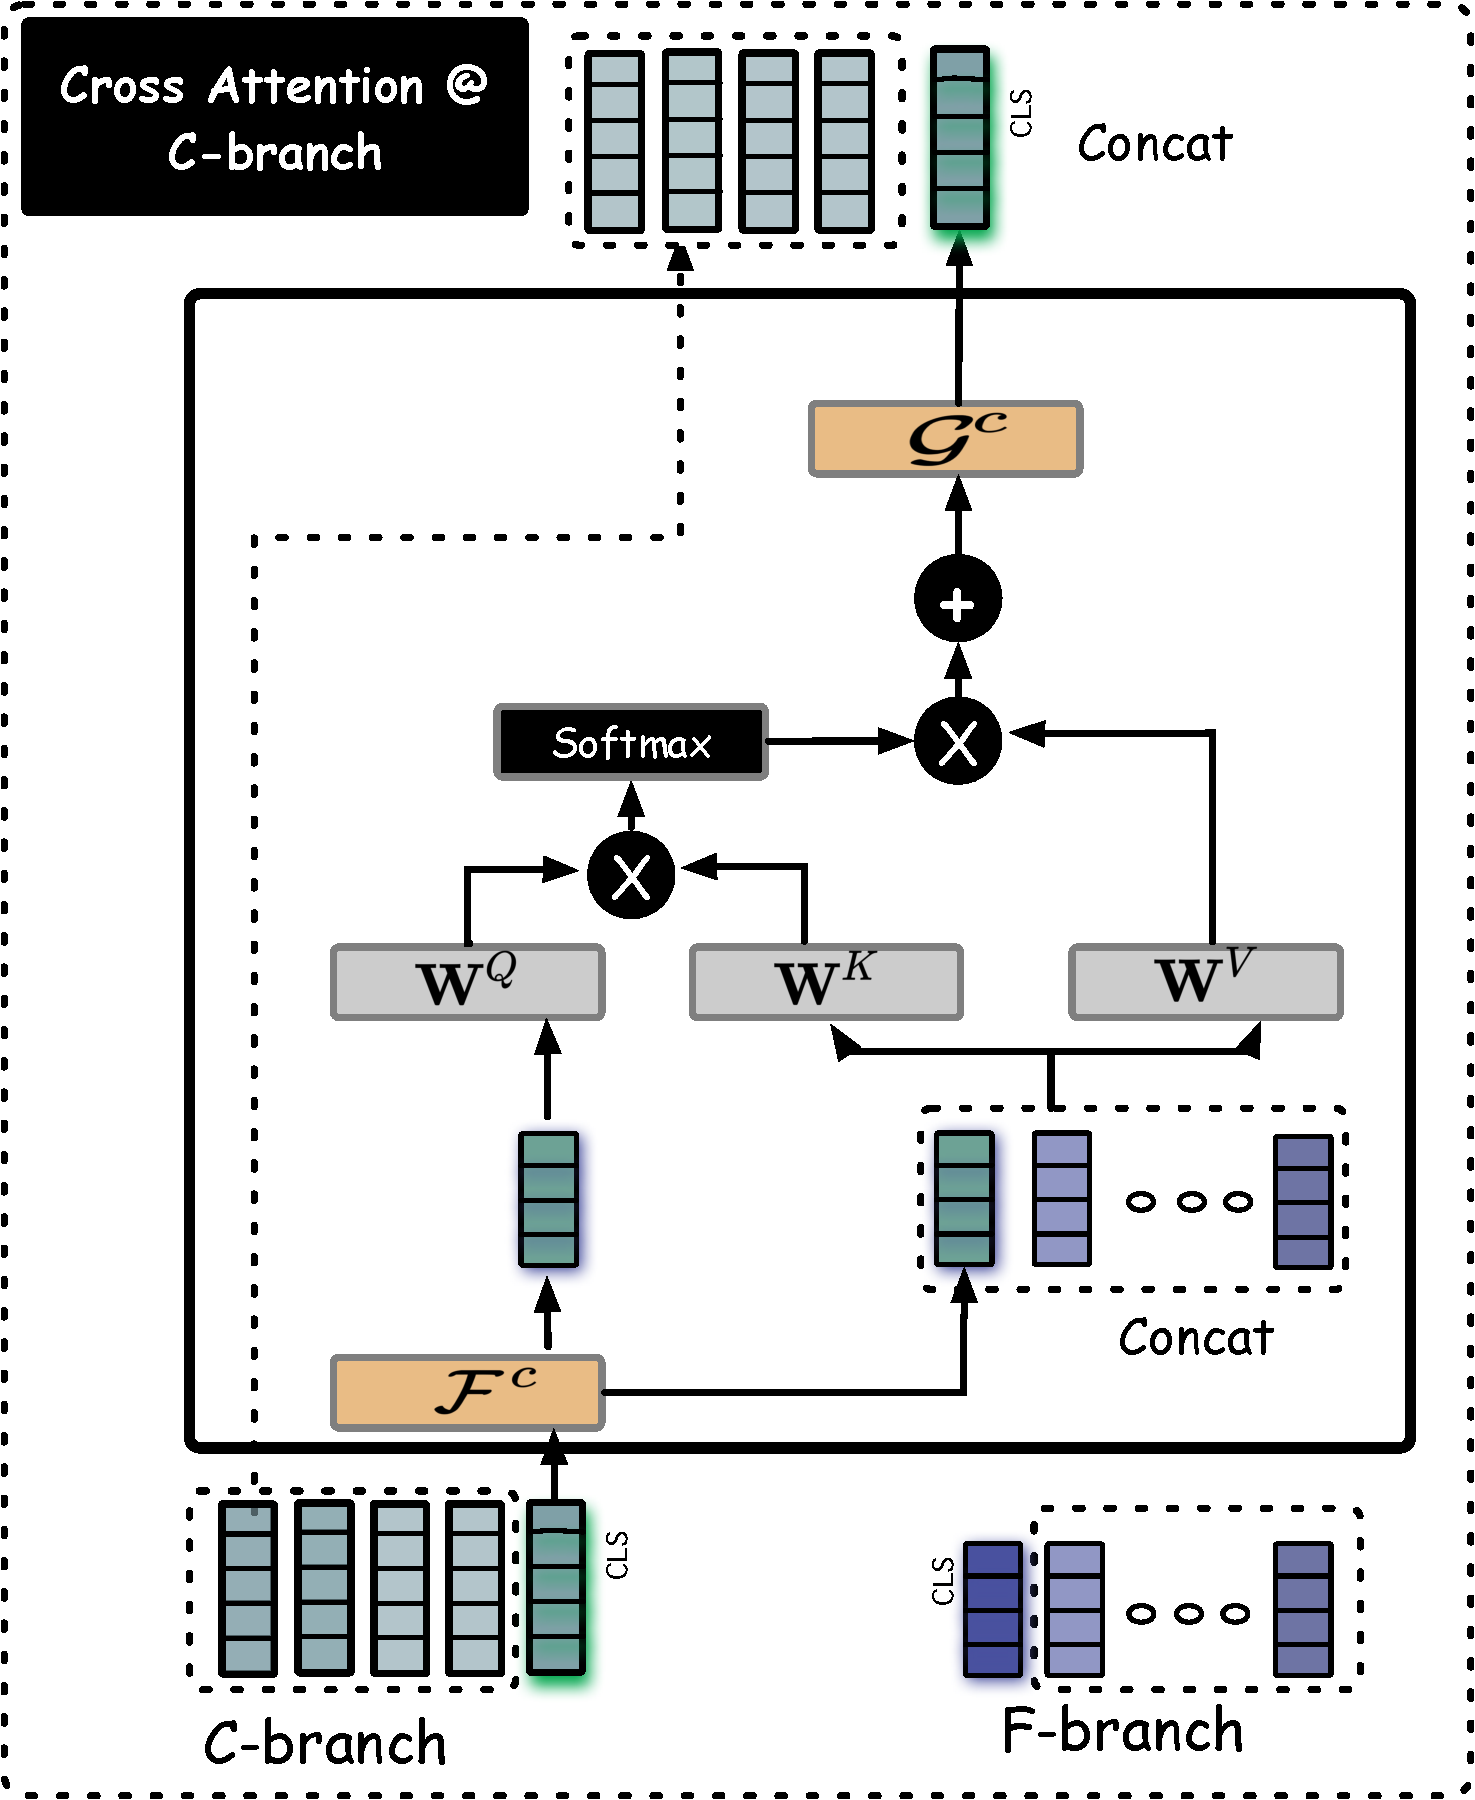
\includegraphics[width=8cm]{05/main3.pdf} \\
  \bicaption[跨尺度特征学习]
    {\textbf{C-branch}的跨尺度自注意力机制。}
    { The cross attention mechanism for the \textbf{C-branch}.}
 \label{fig:mainapq3}
\end{figure} 



\textbf{传统Vision Transformer的背景知识:} Vision transformer (ViT)~\cite{dosovitskiy2020image}通过先将图片分割成一个块序列, 随后将二维的拉平成一个向量, 通过线性映射来将它们映射成token $\mathbf{x}_{patch}$。我们在序列的头部额外添加一个用于分类 \textit{CLS}的token $\mathbf{x}_{cls}$, 用于学习作为分类的表征。类似于传统的Transformer, ViT 对每一个token添加了对应的位置编码来学习二维位置信息。随后, 所有的token被输入进传统的Transformer编码器, 此编码器一般包含多个block。每一个block包含一个多头注意力机制(Multi-headed Self-attention, MSA)以及一个全连接层。同时, 在每一层前都会进行层标准化的操作, 并且在每一层后会使用残差连接。ViT的第一层的输入 $\mathbf{x}_0$以及第$i$层的计算可以用公式写为:
\begin{equation}
    \begin{aligned}
    &\mathbf{x}_{0}=\left[\mathbf{x}_{cls} \| \ \mathbf{x}_{\text{patch}}\right]+\mathbf{x}_{\text {pos }} \\
    &\mathbf{y}_{i}=\mathbf{x}_{i-1}+\mathbf{MSA}\left(\mathbf{LN}\left(\mathbf{x}_{i-1}\right)\right) \\
    &\mathbf{x}_{i}=\mathbf{y}_{i}+\mathbf{FFN}\left(\mathbf{LN}\left(\mathbf{y}_{i}\right)\right)
\end{aligned}
\end{equation}
其中$x_{cls} \in \mathbb{R}^{1\times C}$ , $x_{patch} \in \mathbb{R}^{N\times C}$ and $x_{pos} \in \mathbb{R}^{(1+N) \times C}$分别是 \textit{CLS} token, 图片块 token以及每一个token的位置编码。而 $N$ 和 $C$则是图片块的数量以及嵌入编码的维度。 \par
\textbf{双支网络特征学习}
对于Vision Transformer而言, 切割的图片块的大小和模型最后的准确性以及计算复杂度紧密相关。一般来说, ViT在图片块切割较小数量较多的情况下可以学习到更加细粒度的特征, 从而取得更加优异的性能。但是, 这样的切割通常会导致显著的内存消耗增长以及计算量的增长。如Chen等人\cite{chen2021crossvit}指出, 当图片快大小为$16$时, ViT的性能可以超越图片块为$32$ 的情况接近$6\%$。 但是同时, 它也需要接近4倍的计算开销。 为了在获得更加细粒度的特征表示的同时防止模型复杂度的爆炸性增长, 我们采用了一个双支的ViT, 如图~\ref{fig:mainapq1}所示。具体来说, 在多尺度Transformer内部由下面两个分支: (1)  \textbf{C-Branch}: 是一个采取大图片块切割策略的分支, 用于学习粗粒度的特征。 (2) \textbf{F-branch}: 是一个采取较小图片块的分支, 用于学习更加细粒度的特征。 每一个分支后都是使用得标准的Transformer 编码器。 为了平衡两个分支的计算, 我们通常对于\textbf{C-Branch} 会采取较多的block, 而对于\textbf{F-branch}则会使用较少的。\par
\textbf{跨尺度特征融合} \quad
由于本章设计的目标是为了学习多尺度的判别性特征, 我们需要充足有效的融合来自由两个分支的特征。为了实现这一目的, 我们采取了额外的跨尺度特征融合策略使得每一个分支可以和另一个分支交换信息。具体做法是, 每一个分支的\textit{CLS} token用来和另一个分支的除\textit{CLS}外的token进行交互, 来学习到另一个分支信息。如图~\ref{fig:mainapq3}所示, 以\textbf{C-branch}为例, 为了使\textbf{C-branch} 的\textit{CLS}token包含来自\textbf{F-branch}的信息, 我们将\textbf{C-branch} 的\textit{CLS} token和 来自\textbf{F-branch}的块token进行拼接:
\begin{equation}
    \mathbf{x}^{\prime c}=\left[\mathcal{F}^{c}\left(\mathbf{x}_{c l s}^{c}\right) \ || \ \mathbf{x}_{\text {patch }}^{f}\right]
\end{equation}
其中$\mathcal{F}^c$ 是一个线性映射, 用于对齐两个分支的特征的维度。随后, 我们对\textit{CLS}向量$\mathbf{x}_{cls}^c$使用交叉注意力(Cross-attention, CA)来生成一个融合的特征。通过将 $\mathbf{x}_{cls}^c$ 作为唯一的query向量, 这个注意力可以生成一个新的 \textit{CLS} token, 其充分融合了来自\textbf{F-branch}的细粒度特征。  \textbf{CA} 以及对应的多头交叉注意力(Multi-headed Cross Attention, MCA)如下式所示:
\begin{equation}
    \begin{aligned}
    \textbf{ MCA }(Q, K, V) &=\text { concat }\left(\textbf{head}_{\ 1}, \ldots, \textbf{head}_{\ \mathrm{h}}\right) W^{O} \\
    \text { where \quad \textbf{head}}_{\ \mathrm{i}} &= \textbf{CA }\left(Q \mathbf{W}_{i}^{Q}, K \mathbf{W}_{i}^{K}, V \mathbf{W}_{i}^{V}\right) \\
    \textbf{ CA }(\textbf{q}, \textbf{k}, \textbf{v})  &= \operatorname{softmax}\left(\frac{\textbf{q} \textbf{k}^{T}}{\sqrt{d}}\right) \textbf{ v}
    \end{aligned}
\end{equation}
其中$Q = \mathbf{x}_{cls}^{c}$, $K = \mathbf{x}^{\prime c}$ 并且 $V = \mathbf{x}^{\prime c}$。$\mathbf{W}^Q_i$,~$\mathbf{W}^K_i$,~$\mathbf{W}^V_i \in \mathbb{R}^{d/h}$是可以训练的注意力的参数矩阵。 $d$ 和 $h$则是嵌入的维度以及多头注意力的头数。随后, 对于来自粗粒度分支\textbf{C-branch}的 $\mathbf{x}^c$ 的跨尺度特征融合则可以表示如下:
\begin{equation}
    \begin{aligned}
\mathbf{y}_{c l s}^{c} &= \mathcal{F}^{c}\left(\mathbf{x}_{c l s}^{c}\right)+\textbf{MCA}\left(\textbf{LN}\left(\left[\mathcal{F}^{c}\left(\mathbf{x}_{c l s}^{c}\right) \ \| \ \mathbf{x}_{\text {patch }}^{f}\right]\right)\right) \\
\mathbf{z}^{c} &=\left[\mathcal{G}^{c}\left(\mathbf{y}_{\text {cls }}^{c}\right) \ \| \ \mathbf{x}_{\text {patch }}^{c}\right]
\end{aligned}
\end{equation}
其中 $\mathbf{z}^c$是跨尺度特征融合的输出而$\mathcal{F}^c$ and $\mathcal{G}^c$则是为了对其两个分支的维度的一个前向线性映射和一个反向线性映射。\par
\textbf{可训练的乘积量化网络层}\quad
在Transformer网络的最终, 我们通过融合来自两个分支的 \textit{CLS} token得到了一个最终的特征向量 $\mathbf{x}$。在两个分支的输出均使用线性映射来对齐两个分支的特征维度:
\begin{equation}
    \mathbf{x} = \mathcal{F}_{ln}^c(\mathbf{x}^c_{cls}) + \mathcal{F}_{ln}^c(\mathbf{x}^f_{cls}) = (\mathbf{x}^c_{cls} W_c^T + \mathbf{b}_c) + ( \mathbf{x}^f_{cls} W_f^T + \mathbf{b}_f)
\end{equation}
其中$ \mathbf{x}$是需要被量化的特征向量。$W_c \in \mathbb{R}^{L \times d^c }$ 和  $W_f \in \mathbb{R}^{L \times d^f}$ 则是两个分支的线性映射的权重矩阵。而 $\mathbf{b}_c, \mathbf{b}_f \in \mathbb{R}^{L}$则是对应的偏差参数。$d^c$ 和 $d^f$是  \textbf{C-branch} 和 \textbf{F-branch}的嵌入的维度。 传统的使用 $\argmin$的量化方法, 如下式~\ref{eq:soft}所示, 是不可导的。为了将乘积量化的过程融合进Transformer神经网络架构进行端到端的基于梯度下降的学习, 受这些工作\cite{arandjelovic2016netvlad,yu2018product}的启发, 我们观察到下面的等式:
\begin{equation}
    \label{eq:soft}
    \begin{aligned}
    \mathcal{Q}_{soft}\left(\mathbf{x}_{m}\right) &=\lim _{\gamma \rightarrow+\infty} \sum_{k} \frac{e^{-\gamma\left\|\mathbf{x}_{m}-(z_m^s)_k\right\|_{2}}}{\sum_{k} e^{-\gamma\left\|\mathbf{x}_{m}-(z_m^s)_k\right\|_{2}}} (z_m^s)_k \\
    & = \argmin_{(z^s_m)_k} ||\mathbf{x}_m^s - (z^s_m)_k ||_2^2  \\
    &\text { s.t.}  \quad k \in  \{i\}_{i=0}^{i=K-1}
    \end{aligned}
\end{equation}
当 $\gamma \rightarrow+\infty$时,  第$m$个子向量 $x_m$被量化到在第$m$本\textit{sub-codebook}  $\mathcal{Z}_m^s$ 中最近的\textit{sub-codeword}。其中$K$ 是 $\mathcal{Z}_m^s$中 \textit{sub-codeword}的数量。\par
基于这些发现, 我们设计了本章的软量化器如下:
\begin{equation}
    \mathcal{Q}_{soft}(\mathbf{x_m}) = \sum_{k} \frac{e^{-\gamma \mathcal{D}_E(\mathbf{x}_{m},(z_m^s)_k)}}{\sum_{k} e^{-\gamma \mathcal{D}_E(\mathbf{x}_{m},(z_m^s)_k)}} (z_m^s)_k 
\end{equation}
其中$\mathcal{D}(x,z)$是欧式距离函数。 本章采取一个较大的$\gamma$来使得\textit{softmax}函数逼近原先的\textit{argmin}。软量化器$\mathcal{Q}_{\text{soft}}$ 是可导的, 可以直接被嵌入进深度神经网络中进行训练。\par
具体而言, 我们提出一个可以训练的{PQ} \textit{codebook} $\mathcal{Z}$, 其是一个新分配的用于存储$M$\textit{sub-codebooks}的内存。 每一个\textit{sub-codebook}是一个$K \times \frac{L}{M}$的张量。 \textit{codebook}在最初是随机初始化并且设置成可以学习。这样的话可以通过标准的反向传播算法进行优化。因此, 对于一个特征向量$\textbf{x}$, 我们可以由下式获得其量化后的向量$q$:
\begin{equation}
    \label{eq:quantizer}
        \textbf{q} = [\mathcal{Q}^1_{soft}(x^s_1),\cdots,\mathcal{Q}^m_{soft}(x^s_m),\cdots,\mathcal{Q}^M_{soft}(x^s_M)]
    \end{equation}
    
\subsection{平均精度量化学习}
为了进行同时的量化学习以及特征学习, 我们提出了一个新型的直接优化评价指标\textbf{AP}的量化损失函数。 \par
\textbf{针对非对称检索的平均精度}: 由于基于乘积量化的大规模图像检索一般在测试阶段采取非对称的检索策略, 我们将非对称的检索本质嵌入进我们的量化损失函数中。具体来说, 对于一个具有$N+1$张训练图片 $\mathcal{B}=\left\{I_{1}, \ldots, I_{N+1}\right\}$的训练数据集, 以及其对应的监督标签, 我们可以获得一系列的未量化的特征向量$\mathcal{D} = \left\{ \mathbf{x}_{1}, \ldots, \mathbf{x}_{N+1} \right\}$以及
一系列的量化后的的特征向量 $\mathcal{R} = \left\{ \mathbf{q}_1, \ldots, \mathbf{q}_{N+1} \right \}$。我们将每一个未量化的特征向量$\mathbf{x}$当作一个潜在的检索向量,将所有的除检索向量外的对应的量化后的特征向量当成被检索数据库。 随后, 我们根据每一个在$\mathcal{R}$中的向量和 $\mathbf{x}$的欧式距离
$\mathcal{D}_E$ 进行排序, 得到一个排序序列。 平均精度(AP) 则可以用公式描述为:
\begin{equation}
    \mathbf{AP}=\sum_{i=1}^{N} Prec(i) \ \Delta Rec(i)
    \end{equation}
其中 $Prec(i)$ 和 $Rec(i)$ 是在排序序列$i$ 处的准确率以及召回率。其中$\Delta Rec(i) = Rec(i) - Rec(i-1)$。 值得注意的是,  和Cakir等人一致, 为了方便计算, 我们假设 $Rec(0) = Prec(0) =  0$。

\textbf{AP 的近似计算}: 如Boyd所言 \cite{boyd2013area}, 当$|\mathcal{R}^{+}|$ 时, \textbf{AP} 可以被视为准确率-召回率曲线下的面积(~\textbf{AUPR}).
\begin{equation}
    \label{eq:appro}
    \begin{aligned}
    \textbf { AUPR } &=\int_{0}^{1} Prec(Rec) \ d Rec \\
    &=\lim _{\left|\mathcal{R}^{+}\right| \rightarrow \infty} \sum_{i=1}^{N} \operatorname{Prec}(i) \triangle \operatorname{Rec}(i)
    \end{aligned}
\end{equation}
其中$\mathcal{R}^{+} \subset \mathcal{R}$ 是返回的检索集合 $\mathcal{R}$中的和查询图片是属于同一个类别的集合。相对应的$\mathcal{R}^{-}$则是不属于同一个类别的集合。 如 公式~\ref{eq:appro}所示, 准确度(precision)和召回率(recall)可以看做和查询的数据$\mathbf{x}$的欧式距离的函数。这提供了一个新的绕过在\textbf{mAP}中不可导的排序操作的方法。用 $e$来表示查询向量 $\mathbf{x}$ 和被检索数据库中量化后的$\mathbf{q} \in {\mathcal{R}}$ 之间的欧式距离, 其值域为 $\Omega$。 我们可以重新将平均精度~\textbf{AP}用公式描述为:
\begin{equation}
    \label{eq:ap}
     \textbf{AP} = \int_{\Omega}Prec(e) \ dRec(e)
\end{equation}
为了求解式~\ref{eq:ap}, 受cakir的工作\cite{cakir2019deep}的启发, 我们定义了几个概率函数。首先, 让 $\mathcal{E}$ 作为一个随机变量, 代表欧式距离$e$。我们随后定义两个先验分布 $P(\mathcal{R}^{+})$和$P(\mathcal{R}^{-})$, 其中 $P(\mathcal{R}^{+}) = 1 - P(\mathcal{R}^{-})$。$P(\mathcal{R}^{+})$ 表示对于在被检索集合$\mathcal{R}$中, 给定一个查询$\mathbf{x}$ 的正样本的概率。然后, 我们定义随机变量 $\mathcal{E}$ 的概率密度累计函数(Cumulative Distribution Function, CDF)为:$\mathcal{E}$ as $F(e) = P(\mathcal{E} \le e)$。 \par
有了如上的概率密度函数, 我们可以以一种概率密度函数的角度重新定义Precision 和Recall:
\begin{equation}
    \label{eq:bayesian}
    \begin{aligned}
    \operatorname{Prec}(e)=P\left(\mathcal{R}^{+} \mid \mathcal{E}<e\right) 
    &=\frac{F\left(e \mid \mathcal{R}^{+}\right) P\left(\mathcal{R}^{+}\right)}{F(e)} \\
    \end{aligned}
    \end{equation}
\begin{equation}
\operatorname{Rec}(z)=P\left(\mathcal{E}<e \mid \mathcal{R}^{+}\right)=F\left(z \mid \mathcal{R}^{+}\right)
\end{equation}
公式~\ref{eq:bayesian} 可以通过贝叶斯理论来推到得到。通过在式~\ref{eq:ap}中替换这些, 我们可以得到\textbf{AP}的一个表达式如下:
\begin{equation}
    \label{eq:approb}
    \begin{aligned}
    \textbf{AP} &=\int_{\Omega} P\left(\mathcal{R}^{+} \mid \mathcal{E}<e\right) d P\left(\mathcal{E}<e \mid \mathcal{R}^{+}\right) \\
    &=\int_{\Omega} \frac{F\left(e \mid \mathcal{R}^{+}\right) P\left(\mathcal{R}^{+}\right)}{F(e)} p\left(e \mid \mathcal{R}^{+}\right) d e .
    \end{aligned}
\end{equation}
值得注意的是, 我们是用来如下等式:
\begin{equation}
    dP(\mathcal{E} \le e \mid \mathcal{R}^{+}) = P(e \mid \mathcal{R}^{+}) de
\end{equation}
因为\textbf{CDF}的梯度就是对应的概率密度函数\textbf{PDF}。\par 
由于直接优化公式~\ref{eq:approb}是无法求解的, 我们采取有限和(finite sums)问题来近似的解决。具体来说, 我们先$l2$标准化原始的特征 $\mathbf{x}$以及对应的量化后的特征$\mathbf{q}$。通过这种方法, 值域 $\Omega$ 就限定在了 $[0,2]$之间。 随后, 我们将区间$[0,2]$等分成$L$个相同大小的区间, 每个区间中心为
$\{c_1, \ldots, c_L\}$。这样可以生成直方图 $\mathcal{E} = [e_1,\ldots,e_L]$。我们将离散的\textbf{AP}的近似形式表示为:
\begin{equation}
    \label{eq:approap}
    \text { DAP }=\sum_{e \in \mathcal{E}} \frac{F\left(e \mid \mathcal{R}^{+}\right) P\left(\mathcal{R}^{+}\right)}{F(e)} P\left(e \mid \mathcal{R}^{+}\right)
\end{equation} \par
为了求解公式~\ref{eq:approap}, 我们可以重写这个直方图表示。如Cakir中 \cite{cakir2019deep}的做法, 我们也创建一个距离直方图表示, 每一个桶的中心为 $e_i \in \mathcal{E}$。 $m_j$ 是进入第$j$个桶的数量,  $M_j = \sum_{h\leq j}m_h$是直方图的累积和。 同时, 我们用 $k_j^{+}$ 表示对于查询向量$\mathbf{x}$检索得到的量化后的特征向量的数量, 以及用$M_j^+$表示其累积和。通过这种方法, 我们用这些直方表示概率密度函数如下:
\begin{equation}
    \begin{aligned}
         P(\mathcal{R}^{+}) = \frac{N_{x}^{+}}{N}, \quad P(e \mid \mathcal{R}^{+}) = \frac{m_j^{+}}{N_{x}^{+}} \\
         F(e \mid \mathcal{R}^{+}) = \frac{M_j^+}{N_x^+},\quad F(e) = \frac{M_j}{N}
    \end{aligned}
\end{equation}
其中$N$是被检索数据库$\mathcal{R}$中的向量的数量。 $N_{x}^{+}$是对于查询向量$\mathbf{x}$的正样本检索子集 $\mathcal{R}^{+}$的基数。通过用以上的定义来替代式\ref{eq:approap}中的概率密度函数, 我们可以将\textbf{AP} 重新表示为: 
\begin{equation}
    \label{eq:binn}
    \text { DAP }=\sum_{j=1}^{L} \frac{\frac{M_{j}^{+}}{N_{x}^{+}} \cdot \frac{N_{x}^{+}}{N}}{\frac{M_{j}}{N}} \cdot \frac{m_{j}^{+}}{N_{x}^{+}}=\frac{1}{N_{x}^{+}} \sum_{j=1}^{L} \frac{M_{j}^{+} m_{j}^{+}}{M_{j}}
    \end{equation} \par
\textbf{Soft binning 函数}: 优化公式\ref{eq:binn}还面临一个难题, 即$m_j$ 是通过一个不可导的指示函数生成。为了更好的阐述, 我们接下来仔细的介绍一下直方的生成过程。 对于一个$l2$标准化的检索向量$\mathbf{x}$, 以及一个 被检索的量化后的向量集合$\mathcal{R} = \{q_i,\ldots,q_N\}$。如之前所述, 我们将欧式距离的值域量化成$L$个中心为 $\{c_1, \ldots, c_L\}$的大小相同的桶。 传统的histogram binning 方法如下所示:
\begin{equation}
    \label{eq:indica}
    h_{j}=\sum_{q \in \mathcal{R}} \mathbb{1}\left[Q(\mathbf{q})=j\right]
    \end{equation}
其中 $\mathbb{1}$是一个指示函数, 而 $Q$可以进一步表示为:
\begin{equation}
    Q(\mathbf{q})=\arg \min _{i}\left|\mathcal{D}_E\left(\mathbf{x}, \mathbf{q}\right)-c_{i}\right|, \forall \mathbf{q} \in \mathcal{R} 
\end{equation}
其中 $\mathbf{D}_E$ 是欧式距离函数。 由于指示函数~\ref{eq:indica}是不可导的, 如Revaud的做法\cite{revaud2019learning}, 我们定义了一个软binning 函数  $\delta$。 $\delta(x,j)$ 是一个三角核函数, 其中心为第$j$个桶的中心$c_i$, 并且其宽度为$\Delta = c_j - c_{j-1}$:
\begin{equation}
    \delta(x, j)=\max \left(1-\frac{\left|x-c_{j}\right|}{\Delta}, 0\right)
\end{equation}
值得注意的是在桶的数量趋向于无穷大$L \rightarrow \infty $时候, 软binning函数 $\delta(x,i)$逐渐接近指示函数\ref{eq:indica}。 最重要的是, 它对于 $x$ 可导。因此, 我们可以将传统的不可导的binning操作~\ref{eq:indica} 重写为:
\begin{equation}
    \label{eq:indicasoft}
    \hat{h}_{j}=\sum_{q \in \mathcal{R}} \delta(\mathcal{D}_E(\mathbf{x},\mathbf{q}), j)
\end{equation} \par
\textbf{总共的优化}: 在训练阶段, 由于直接在整个数据集上进行计算检索的\textbf{AP}并不可行, 我们随机从训练数据集中采样出小的批次数据。我们用 $\mathcal{B}=\left\{I_{1}, \ldots, I_{B}\right\}$代表训练数据的标签, 用 $\mathcal{D} = \left\{ \mathbf{x}_{1}, \ldots, \mathbf{x}_{B} \right\}$ 代表对应图片的特征向量, 以及$\mathcal{R} = \left\{ \mathbf{q}_{1}, \ldots, \mathbf{q}_{B} \right\}$代表对应的量化后的向量。 随后, 我们提出的平均精度量化损失函数(\textbf{APQ})可以用下式表示:
\begin{equation}
    L_{\textbf{APQ}} = - \frac{1}{B}\sum_{i=1}^{B} \ \mathbf{AP}(\mathbf{x_i}, \mathcal{R} \backslash \mathbf{q}_i)
\end{equation}\par
\textbf{检索过程}: 当\textbf{APQFormer}经过基于随机梯度下降的端到端神经网络训练优化后, 对于每一张在被检索数据集中的图片$I$, 我们可以通过神经网络得到对应的特征向量$\mathbf{x}$。随后, 对每一个子向量 $x_m^s$, 我们计算它和对应的 \textit{sub-codewords}$\{ (c_m^s)_k \}_{k=1}^{k=K}$的欧式距离。 然后, 找到和子向量欧式距离最近的 \textit{sub-codeword} $(c_m^s)_k$的索引。 我们随后可以用一个 $\log_2 (K)$位的二进制码来代表$k$, 这便是对于子向量$x_m^s$的二进制量化编码 $b_m^s$ 。
对于$\it{I}$的二进制编码$b \in \{0,1\}^{M*\log_2(K)}$ 是所有子二进制编码 $[b_1^s,\ldots,b_M^s]$的拼接。 我们重复这个过程, 直到计算完并且存储所有在检索数据集中图片的二进制量化编码表示。\par
\textbf{非对称检索}:  
给定一张查询图片$\it{I}_q$, 以及一个检索的二进制量化编码数据集, 我们遵循\textbf{DQN}中的做法采取非对称量化距离(Asymmetric Quantizer Distance, AQD)作为相似度度量工具。对于查询图片$\it{I}_q$和一个被检索的图片$\it{I}_r$, \textbf{AQD}的计算如下:
\begin{equation}
    \mathbf{AQD}(I_q,I_r) = \sum_{m=1}^{M} || (\mathbf{x}_m^s)_q - \mathcal{C}_m (b_m^s)_r |||
\end{equation}
其中 $\mathbf{x}_q$ $\it{I}_q$的特征向量而 $b_r$则是对应被检索图片$\it{I}_i$的二进制量化编码。$\mathcal{C}_m$ 是对应的\textit{sub-codebook}。$(\mathbf{x}_m^s)_q$和 $b_m^s$是$\mathbf{x}_q$和$b_r$对应的第$m$个子向量以及第$m$个子量化编码。
由于距离的计算是在一个特征向量和一个量化后的特征向量之间进行, 所以视为非对称的距离计算。 在实际检索场景中, \textbf{AQD} 的计算可以通过预先计算子向量$x_m^s$和在\textit{sub-codebook} $\mathcal{C}_m$ 的所有\textit{sub-codewords} 的欧式距离, 并且将它们存储在 $M \times K$的查询表中。 随后, 对于查询向量和一个被检索的向量的距离计算, 我们只需要进行 $M$ 次查表以及相加的操作。 同时, 基于倒排索引\cite{babenko2014inverted}等传统用于大规模向量检索的近似最近邻搜索的方法也可以用于加速此场景。

\begin{table}[!htpb]
    %% \centering % not needed
    \bicaption{各个先进深度哈希算法在\textbf{CIFAR-10}上的测试结果}{Results of state-of-the-art deep hashing methods on \textbf{CIFAR-10}}
    \centering
    \begin{tabular}{cccccc}
       \\ \hline
    \multicolumn{2}{l|}{Methods} & 16-bit & 32-bit  & 64-bit   \\\hline
    \multicolumn{2}{l|}{DSH} & 69.1 & 67.0   & 52.4  \\  
    \multicolumn{2}{l|}{HashNet} & 55.5 & 86.8 & 88.0   \\  
    \multicolumn{2}{l|}{GreedyHash} & 81.5 & 83.5 & 86.3   \\  
    \multicolumn{2}{l|}{CSQ} & 83.6 & 82.8 & 83.7  \\  
    \multicolumn{2}{l|}{DPN} &  82.0 & 83.8 & 82.0   \\  
    \hline
    \hline
    \multicolumn{2}{l|}{DQN} & 63.5 & 65.5 & 66.7   \\
    \multicolumn{2}{l|}{DTQ} & 80.1 & 82.3 & 82.5   \\
    \multicolumn{2}{l|}{PQN} & 73.5 & 75.5 & 78.5  \\
    \multicolumn{2}{l|}{GPQ} & 78.8 & 82.3 & 83.5  \\
 
    \hline
    \hline
     \multicolumn{2}{l|}{\textcolor{red}{APQFormer} }&\textcolor{red}{\textbf{88.5}} & \textcolor{red}{\textbf{88.8}} & \textcolor{red}{\textbf{89.1}} \\
     \hline
     \hline
    \end{tabular}
    \label{table:cifar10apq}
  \end{table}

  \begin{table}[!htpb]
    %% \centering % not needed
    \bicaption{各个先进深度哈希算法在\textbf{IMAGENET}上的测试结果}{Results of state-of-the-art deep hashing methods on \textbf{IMAGENET}}
    \centering
    \begin{tabular}{cccccc}
       \\ \hline
    \multicolumn{2}{l|}{Methods} & 16-bit & 32-bit  & 64-bit   \\\hline
    \multicolumn{2}{l|}{DSH} & 47.3 & 67.3   & 75.3  \\  
    \multicolumn{2}{l|}{HashNet} & 20.5 & 47.8 & 66.0   \\  
    \multicolumn{2}{l|}{GreedyHash} & 81.2 & 84.6 & 85.6   \\  
    \multicolumn{2}{l|}{CSQ} & 83.6 & 86.0 & 86.6  \\  
    \multicolumn{2}{l|}{DPN} &  83.3 & 85.7 & 86.6   \\  
    \hline
    \hline
    \multicolumn{2}{l|}{DQN} & 65.6 & 68.5 & 67.8   \\
    \multicolumn{2}{l|}{DTQ} & 78.3 & 81.2 & 83.8   \\
    \multicolumn{2}{l|}{PQN} & 76.6 & 77.4 & 79.2  \\
    \multicolumn{2}{l|}{GPQ} & 78.7 & 82.3 & 85.6  \\
 
    \hline
    \hline
     \multicolumn{2}{l|}{\textcolor{red}{APQFormer} }&\textcolor{red}{\textbf{92.2}} & \textcolor{red}{\textbf{92.4}} & \textcolor{red}{\textbf{92.9}} \\
     \hline
     \hline
    \end{tabular}
    \label{table:imagenetapq}
  \end{table}

\section{实验结果与分析}
在本章节中, 我们首先介绍了使用的数据集的信息, 实验评估的指标。 然后我们介绍了模型实现的细节。随后我们仔细的评估测试了\textbf{APQFormer}在标准数据集上的性能效果以及和先进的算法进行细致的对比。我们随后也进行了细致的消融实验来评估模型各个部分的有效性。
\subsection{数据集信息}
本节的实验采取两个标准的大规模检索数据集-\textbf{CIFAR-10}和\textbf{IMAGENET}进行实验以及比对。为了确保实验的公正与公平, 我们采取标准的训练集和测试集划分的方法。 两个数据集如下:
\begin{enumerate}
    \item \textbf{CIFAR-10}~\cite{krizhevsky2009learning}一共包含了$60,000$张来自$10$个类别的照片。我们随机对于每一个类别采样 $500$张图片来构成训练数据集, 随机采样 $100$张作为查询数据集, 剩余的图片组成了被检索的数据库。 
    \item  \textbf{IMAGENET}~\cite{russakovsky2015imagenet} 是一个训练数据包含了超过120万张图片, 验证数据集包含了超过5万张照片的大规模图像识别数据集。我们遵循Cao等人的实验准则\cite{cao2017hashnet}。 我们先随机采样出$100$个类别, 随后将这些类别在验证集中的所有图片作为查询图片。 这些类别在训练数据集中的所有图片作为数据库。 同时, 我们对每一个类别采样出$100$张图片作为检索任务的训练集合。 
\end{enumerate}


\subsection{评估指标}
我们采取平均准确率均值 (Mean Average precision, mAP) 以及 \textbf{Precision}-\textbf{Recall}  曲线来评估方法的性能。\textbf{CMC}计算查询图片出现在检索返回列表不同位置的概率。由于它仅仅考虑第一次的匹配, 使得其不适用于数据库中包含不止一张与查询图片属于同一辆车的图片的场景。因此我们加入\textbf{mAP}作为评估指标。~\textbf{mAP}同时考虑返回的查询结果的\textit{precison}和\textit{recall}其中 \textbf{mAP}的计算如下
\begin{equation}
   \textbf{mAP} = \frac{1}{n} \sum_{k=1}^{k= N} \textbf{AP}_k
\end{equation}
其中$N$是查询的图片总数。由此式可知, $mAP$则为每张图片的平均准确率的平均值。其中~\textbf{AP}是计算precision-recall曲线下的面积, 如下所示:
\begin{equation}
  \text { AP }^{=} \sum_{k=1}^{N} precision _{i}\left( recall _{k}- recall _{k-1}\right)
\end{equation}

其中 $k \in \{1, 2, 3, ..., N\}$并且$N$是被查询的数据集中照片的总数。
和 Cao等人类似\cite{cao2018deep,cao2017hashnet}, 我们对于\textbf{CIFAR-10}计算其$54,000$张返回图片的\textbf{mAP}, 而对于\textbf{NUSWIDE}和~\textbf{IMAGENET}, 则是计算$5,000$和$1,000$张返回图片。
\subsection{实现细节}
本章的模型基于\textbf{PYTORCH}实现, 所有的实验在两块 NVIDIA RTX 3080TI GPU上完成。对于所有的用来比较的深度哈希算法, 我们采取在\textbf{IMAGENET}上进行预先了的\textbf{ResNet-50}作为主干网络。用来比较的先进深度哈希算法包括, 深度汉明哈希算法:\textbf{DSH}~\cite{liu2016deep},~\textbf{HashNet}~\cite{cao2017deep},~\textbf{GreedyHash}~\cite{su2018greedy},~\textbf{DPN}~\cite{fan2020deep},~\textbf{CSQ}~\cite{yuan2020central} 和深度乘积量化算法: ~\textbf{DQN}~\cite{yue2016deep} ,~\textbf{DTQ}~\cite{liu2018deep}, ~\textbf{PQN}~\cite{yu2018product}, ~\textbf{GPQ}~\cite{jang2020generalized}. \par

\begin{table}[!htpb]
    %% \centering % not needed
    \bicaption{各个不同的变种在三个数据集上的效果}{Results of different variants on three datasets}
    \centering
    \begin{tabular}{cccccc}
       \\ \hline
    \multicolumn{3}{l|}{Datases} & \multicolumn{3}{c}{\textbf{CIFAR-10}} \\
    \multicolumn{3}{l|}{Methods} & 16-bit & 32-bit & 64-bit   \\\hline
    \hline
    \multicolumn{3}{l|}{\textbf{APQFormer}} & \textcolor{red}{88.5} & \textcolor{red}{88.8} &  \textcolor{red}{89.1}  \\
    \multicolumn{3}{l|}{\textbf{APQFormer-C}} & 86.2 &  86.7 &   88.4  \\
    \multicolumn{3}{l|}{\textbf{APQFormer-F}} & 86.6 & 87.1 &  89.0  \\
    \hline
    \hline 
    \multicolumn{3}{l|}{Datases} & \multicolumn{3}{c}{\textbf{IMAGENET}} \\
    \multicolumn{3}{l|}{Methods} & 16-bit & 32-bit  & 64-bit   \\\hline
    \hline
    \multicolumn{3}{l|}{\textbf{APQFormer}} & \textcolor{red}{92.2} & \textcolor{red}{92.4} &  \textcolor{red}{92.9}  \\
    \multicolumn{3}{l|}{\textbf{APQFormer-C}} & 86.6 & 89.7 &  91.0  \\
    \multicolumn{3}{l|}{\textbf{APQFormer-F}} & 86.4 & 90.6 &  91.8  \\
    \hline
    \hline 
    \end{tabular}
    \label{table:abdtq}
  \end{table}



至于模型的细节, 对于 \textbf{F-branch}, 我们将图片分块大小设置为$12$, 嵌入的特征维度设置为$192$。而对于\textbf{C-branch}, 图片分块大小为$16$对应的嵌入特征维度被设置为$384$。框架一共包含$3$个多尺度block, 每一个多尺度block包含了\textbf{F-branch}的$1$个标准的Transformer block 以及 \textbf{C-branch}的$4$ 个Transformer block。同时还包含了一个跨尺度特征融合block来融合两个分支的信息。多头注意力机制的头数被设置为$6$. 为了生成不同长度的二进制量化编码, 我们将\textit{sub-codewords}的数量 $K$设置为$16$, 将 $M$设置为$4, 8, 16$ 来分别获得$16, 32, 64$位的量化编码。 \par
对于训练的细节, 我们采取 \textit{RMSprop}优化器以及of $1e-5$的学习率衰减来优化整个网络模型。 最初的学习率被设置为$1e-5$。控制软量化的 $\gamma$被设置为$20$, 批次数据的大小被设置为$50$。对于\textbf{C-branch}和\textbf{F-branch}, 训练图片分别被随机裁剪到 $240 \times 240$ 和$224 \times 224$。 我们采取标准的数据增光策略来防止模型过拟合, 如 随机上下翻转, 色彩抖动 以及随机放大等。




\subsection{与先进算法的对比结果}
本小节将我们提出的\textbf{APQFormer}框架和先进的深度哈希算法框架进行仔细的性能对比。在两个图像检索的标准数据集上的实验结果如表~\ref{table:cifar10apq}和表~\ref{table:imagenetapq}所示。 很明显可以发现本章提出的算法在平均精度均值(\textbf{mAP})下以大幅度性能领先所有相比较的先进的算法架构。例如, 和先进的深度汉明哈希方法相比较, 我们在\textbf{CIFAR-10}和\textbf{IMAGENET}上三种不同的哈希编码长度上分别取得了平均\textbf{5.43} 和 \textbf{7.09\%}的性能提升。 至于和深度乘积量化的方法相比较, 我们在\textbf{CIFAR-10}和\textbf{IMAGENET}上均超过使用两阶段量化方法的基于三元组的\textbf{DTQ}。 我们平均取得  \textbf{7.16\%}和~\textbf{11.5\%}的\textbf{mAP}的提升。相比较端到端的深度量化方法, 本章提出的算法在两个数据集上以及3种不同的量化编码长度上-\textbf{APQFormer}-仍然是一个明显的赢家。和最先进的端到端的乘积量化方法\textbf{GPQ}相比, 我们在\textbf{CIFAR-10}和\textbf{IMAGENET}上, 分别平均获得了\textbf{7.27\%} 和 \textbf{10.30\%} 的\textbf{mAP}提升。值得注意的是, 和相比较的深度哈希不同的是, 本章提出的算法并不需要繁琐的调试量化损失函数中的超参数。 同时表~\ref{table:cifar10apq}和表~\ref{table:imagenetapq}也揭露了一些有趣的发现: (1) 我们注意到整体来说端到端的量化学习方法取得了更加优异的结果。这是由于乘积量化学习的过程被融合进了神经网络进行有监督的优化。 (2) 汉明哈希模型通常在哈希码长度增加时性能获得提升。 这主要是由于较长的哈希码可以保留更多的判别性特征。 而对于基于量化编码的模型, 较长的哈希码可以更加精确的表示原来的特征空间。 总体来说, 本章提出的模型~\textbf{APQFormer}的优异性能可以归功于两个方面: (1) 基于双支Vision Transformer的乘积量化网络可以端到端的进行多尺度的细粒度特征学习以及同时进行有监督的乘积量化学习。(2) 进行相似度保留的平均精度量化损失函数 (\textbf{APQ} )将非对称的量化检索嵌入进度量学习中, 通过直接优化返回的检索列表的\textbf{AP}, 可以进行更加准确的度量学习。



\begin{figure}[!htp]
  \centering
  \begin{subfigure}{0.45\textwidth}
    \centering
    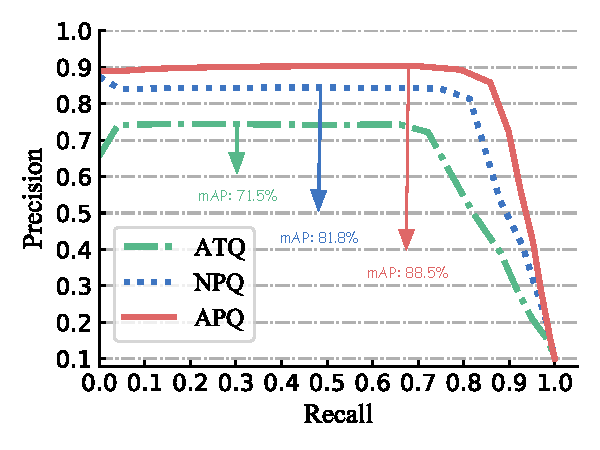
\includegraphics[height=5cm]{05/cifar_16b_anno.pdf}
    \caption{16位哈希码下在\textbf{CIFAR-10}上各种方法的\textbf{PR}曲线}
  \end{subfigure}
  \hspace{1cm}
  \begin{subfigure}{0.45\textwidth}
    \centering
    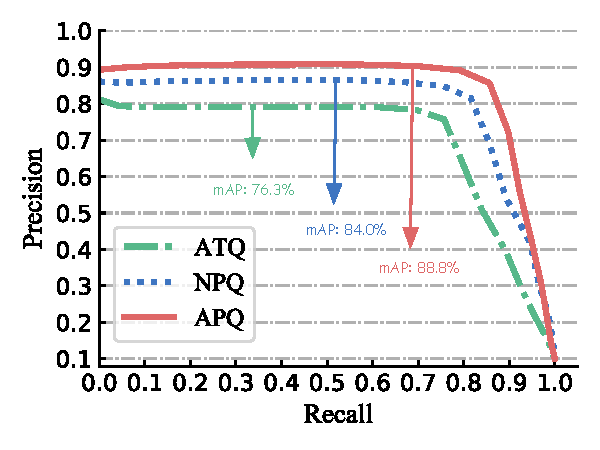
\includegraphics[height=5cm]{05/cifar_32b_anno.pdf}
    \caption{32位哈希码下在\textbf{CIFAR-10}上各种方法的\textbf{PR}曲线}
  \end{subfigure}
  \hspace{1cm}
  \begin{subfigure}{0.45\textwidth}
    \centering
    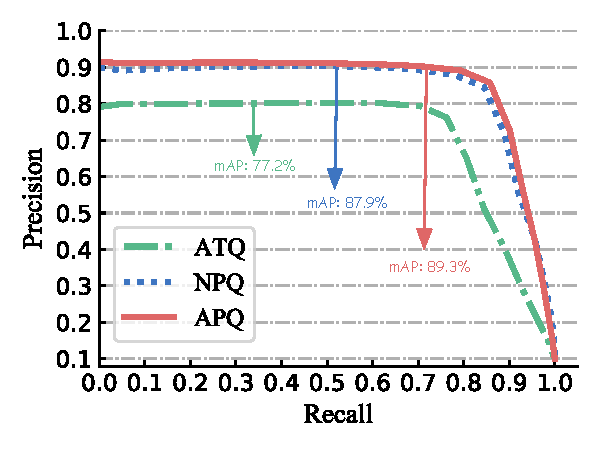
\includegraphics[height=5cm]{05/cifar_64b_anno.pdf}
    \caption{64位哈希码下在\textbf{CIFAR-10}上各种方法的\textbf{PR}曲线}
  \end{subfigure}
  \hspace{1cm}
  \begin{subfigure}{0.45\textwidth}
    \centering
    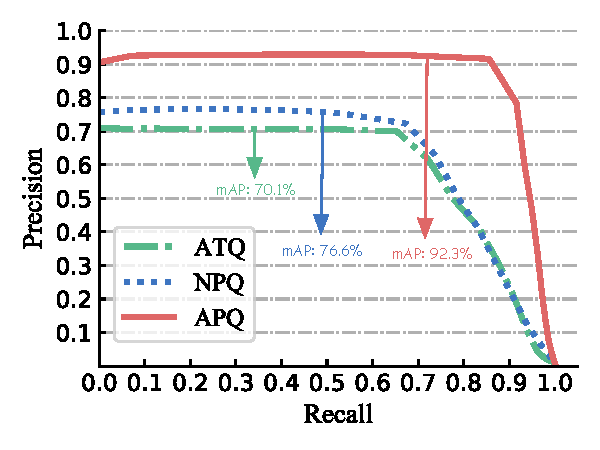
\includegraphics[height=5cm]{05/imagenet_16b_anno.pdf}
    \caption{16位哈希码下在\textbf{IMAGENET}上各种方法的\textbf{PR}曲线}
  \end{subfigure}
  \hspace{1cm}
  \begin{subfigure}{0.45\textwidth}
    \centering
    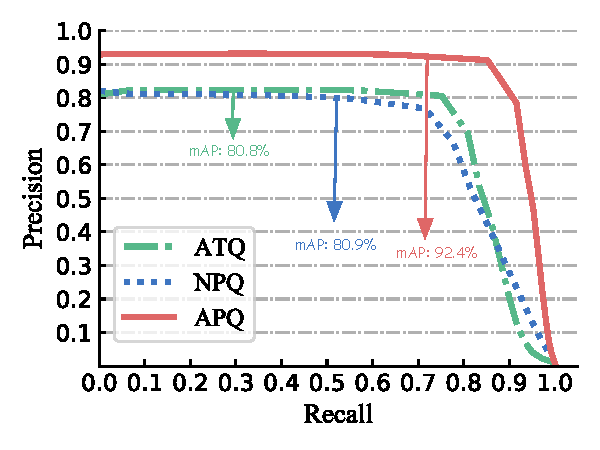
\includegraphics[height=5cm]{05/imagenet_32b_anno.pdf}
    \caption{32位哈希码下在\textbf{IMAGENET}上各种方法的\textbf{PR}曲线}
  \end{subfigure}
  \hspace{1cm}
  \begin{subfigure}{0.45\textwidth}
    \centering
    \includegraphics[height=5cm]{05/imagenet_64b_anno.pdf}
    \caption{64位哈希码下在\textbf{IMAGENET}上各种方法的\textbf{PR}曲线}
  \end{subfigure}
  \bicaption[各种量化损失函数在\textbf{CIFAR-10}和\textbf{IMAGENET}上的结果]{
      \textbf{APQ}量化损失和其他两种量化损失函数在\textbf{CIFAR-10}和\textbf{IMAGENET}数据集上的结果}{The experimental results on \textbf{CIFAR-10} and \textbf{IMAGENET} of \textbf{APQ} and other quantization losses.}
  \label{fig:abloss3}
\end{figure}

\subsection{消融实验}
在本小节, 我们对本章提出的\textbf{APQFormer}的每一个模块的作用进行了仔细的实验分析与研究。具体来说, 我们首先提供了详细的消融实验来研究主干神经网络来证实双支特征学习的必要性。随后, 我们将提出的量化学习损失函数\textbf{APQ} 和两个先进的量化损失函数进行实验来验证\textbf{APQ}损失函数的有效性。 最后, 我们将\textbf{APQ}和\textbf{APQ}基于的\textbf{FastAP}度量学习损失函数进行了比较, 证明非对称量化学习的有效性。\par
\textbf{主干网络的消融实验}: 我们设计了一个详尽的消融实验来验证本章中提出的主干网络的双支学习的有效性。具体来说, 我们设计了两种主干网路的变种:
\begin{enumerate}
    \item \textbf{APQFormer-C}: 一个只包含\textbf{C-branch}的\textbf{APQFormer}的变种。
    \item \textbf{APQFormer-F}: 一个只包含\textbf{F-branch}的\textbf{APQFormer}的变种。
\end{enumerate}
值得注意的是, 我们测量的这两个变种基于同等多的标准的Transformer block 并且其多头注意力的头数也一致。如表~\ref{table:abdtq}所示, 完整的模型~\textbf{APQFormer} 在两个数据集上以及三种不同的哈希长度上以较大幅度的性能差距明显超过其他两种变种。这证明了双支Vision Transformer的特征设计的有效性。 同时, 我们也能观察到~\textbf{APQFormer-F}变种在各种场景下性能优于\textbf{APQFormer-C}。这是由于其采取的图片分块的数量更大, 可以学到更加细粒度的特征。但是值得注意的是, 这也会导致计算量的显著增大。\par
\textbf{和其他的量化损失函数的对比}:  我们额外提供了实验分析证明我们提出的量化损失函数~\textbf{APQ}的有效性。我们和以下两种先进的量化损失函数进行了细致的比较:
\begin{enumerate}
    \item \textbf{ATQ} 是一个由Yu等人\cite{yu2018product}提出的非对称的三元量化损失函数。
    \item \textbf{NPQ} 是有Jang等人\cite{jang2020generalized}提出的用于半监督图像检索场景的n-pair 量化损失函数。
\end{enumerate}


实验结果如图~\ref{fig:abloss3}所示。很明显, 我们提出的量化损失函数~\textbf{APQ}可以以大幅度性能优势领先其余两种量化损失函数。特别来说, 在\textbf{IMAGENET}数据集上, 我们在\textbf{mAP}指标上, 分别超越了\textbf{ATQ} 和\textbf{NPQ} 平均 \textbf{$14.01$}\% 和 \textbf{$10.75$}\%。 在 \textbf{CIFAR-10}数据集上, \textbf{APQ} 也以大幅度领先于\textbf{ATQ} 和 \textbf{NPQ}。在16位哈希码长度下, \textbf{APQ}取得了 $\textbf{88.5\%}$ \textbf{mAP}, 分别超出\textbf{ATQ} 和 \textbf{NPQ} $17.0\%$ 和 $6.7 \%$。在32位哈希码长度下, \textbf{APQ}取得了 $\textbf{88.8\%}$ \textbf{mAP}, 分别超出\textbf{ATQ} 和 \textbf{NPQ} $12.5\%$ 和 $4.8 \%$。同时, 在图~\ref{fig:abloss3}中, 我们也可以观察到 \textbf{APQ}的 \textbf{PR} 曲线始终在其余两个量化损失函数对应的曲线之上, 这进一步证实了我们的损失函数的有效性。\par
\begin{figure}[!htp]
  \centering
  \begin{subfigure}{0.45\textwidth}
    \centering
    \includegraphics[height=5cm]{05/ablation_cifar_16b_anno.pdf}
    \caption{16位哈希码下在\textbf{CIFAR-10}上\textbf{APQ}和\textbf{FastAP}的性能比较}
  \end{subfigure}
  \hspace{1cm}
  \begin{subfigure}{0.45\textwidth}
    \centering
    \includegraphics[height=5cm]{05/absym_imagenet_16b_anno.pdf}
    \caption{16位哈希码下在\textbf{IMAGENET}上\textbf{APQ}和\textbf{FastAP}的性能比较}
  \end{subfigure}
  \hspace{1cm}
  \bicaption[\textbf{FastAP}和\textbf{APQ}量化损失函数的性能比较]{
      \textbf{APQ}和\textbf{FastAP}在两个数据集上性能比较的结果}{The experimental results on two datasets  of \textbf{APQ} and \textbf{FastAP} }
  \label{fig:abapfast}
\end{figure}

\begin{figure}[!htp]
  \centering
  \begin{subfigure}{0.45\textwidth}
    \centering
    \includegraphics[height=5cm]{05/apq_tsne_anno.pdf}
    \caption{16位哈希码下在\textbf{CIFAR-10}上\textbf{APQ}的深度特征t-SNE可视化}
  \end{subfigure}
  \hspace{1cm}
  \begin{subfigure}{0.45\textwidth}
    \centering
    \includegraphics[height=5cm]{05/fastap_tsne_anno.pdf}
    \caption{16位哈希码下在\textbf{IMAGENET}上\textbf{FastAP}的深度特征t-SNE可视化}
  \end{subfigure}
  \bicaption[\textbf{FastAP}和\textbf{APQ}的深度特征t-SNE可视化图对比]{
      \textbf{APQ}和\textbf{FastAP}在\textbf{CIFAR-10}上的深度特征可视化}{The t-SNE Visualization of deep features learned by \textbf{APQ} and \textbf{FastAP} on \textbf{CIFAR-10}}
  \label{fig:abapfast1}
\end{figure}

\textbf{APQ Vs FastAP}。为了进一步分析\textbf{APQ}的性能, 我们进行了一系列其他的实验来将\textbf{APQ}和\textbf{FastAP}进行比较。\textbf{FastAP}~~\cite{cakir2019deep}是设计用来进行通用的度量学习的损失函数。 我们在图~\ref{fig:abapfast}中画出来\textbf{PR} 曲线和~\textbf{mAP}的结果。同时, 我们进一步画出两个损失函数学习到的深度特征的 t-SNE 可视化图~\ref{fig:abapfast1}。很明显, \textbf{APQ} 在\textbf{PR} 曲线和~\textbf{mAP}上持续性的超越了\textbf{FastAP}。同时, 如图~\ref{fig:abapfast1}所示, \textbf{APQ}可以学习到更加紧凑可以区分的深度特征。 
\section{总结}
本章提出了第一个基于Vision Transformer的端到端的乘积量化框架-\textbf{APQFormer}。提出的\textbf{APQFormer}包含了一个双支的基于Vision Transformer的量化主干网络~\textbf{DTQN}。 其可以同时进行多尺度特征学习以及端到端的乘积量化学习。 对于相似度保留的监督训练, 我们提出了一个新型的量化损失函数\textbf{APQ} 直接优化评估指标\textbf{mAP}。我们在标准的数据集上进行了大量的实验。实验结果证实了本章提出的算法的有效性以及和其他基于传统卷积神经网络的量化方法相比较的优越性。
% !TEX root = ../main.tex
\chapter{总结与展望}
\section{本文工作总结}
随着互联网技术, 数字成像技术, 多媒体技术的蓬勃发展, 以及各种社交网络的兴起, 网络上的数字图像内容数量呈现爆炸性的速度的增长。如何对海量的图片进行处理与分析成为了现代社会一个急切的需求。大规模图像检索算法是对海量图片进行处理分析的基石, 由于其在智能安防, 电商搜图, 智能医疗等多个领域具有重要的应用价值, 图像检索技术在近年来获得了工业界以及学术界广泛的关注。然而针对真实的应用场景比如行人检索, 以及大规模的图像检索问题, 仍然是现在技术研究的主要瓶颈。 \par
针对上述的问题, 受到近年来深度哈希技术的研究的启发, 本文主要研究了深度哈希技术在大规模图像检索领域的应用。我们针对两种图像检索的现实应用-行人检索以及车辆检索进行探索。 同时, 受Vision Transformer在图像识别领域超越卷积神经网络的启发,我们探究了基于Vision Transformer的深度哈希技术在通用大规模图像检索的应用, 并且提出了两个新型的框架创新。本文提出的基于Vision Transformer的深度哈希框架是深度哈希领域第一个不基于卷积神经网络的框架, 具有理论意义以及较为显著的应用价值。 本文的主要创新点以及成果如下:\par
(1) 基于恒定特征学习的跨模态行人检索算法 \par
传统行人重识别检索问题针对单模态数据, 由于模态鸿沟的存在, 无法被直接应用到跨模态行人重识别检索的场景下。 针对这一问题, 本文第二章提出了一个跨模态行人重识别检索的框架-\textbf{MAENET}。我们创新性的基于自编码器提出了一个神经网络结构来学习对不同模态恒定以及外表恒定的特征。 同时, 我们设计了适用于跨模态检索对齐不同模态特征的损失函数, 使得网络可以在动态创建的图片对上进行监督训练。第二章提出的框架在多个跨模态检索数据集上取得了优越的性能表现, 证明了算法的有效性。\par 
(2) 基于深度哈希的大规模车辆检索算法 \par
传统的车辆重识别检索方法基于实值向量, 虽然可以取得较高的检索精度, 但是由于其存储开销大和检索速度慢, 无法适应真实环境的大规模车辆检索场景中。 本文第三章提出了第一个基于深度哈希的大规模车辆检索框架。通过提出了一个新型的离散哈希模块来进行离散的哈希码生成, 以及一个基于困难三元组的损失函数进行特征学习。本文第三章提出一个交替优化的算法来进行整个框架的优化。在主流的车辆重识别数据集上进行的四种不同哈希码长度的性能测试, 第三章提出的算法都显著超越了当前的普适哈希算法。 \par
(3) 基于Vision Transformer的深度哈希检索框架 \par
为了进一步优化深度哈希算法的表征能力, 本文第四章第一个探索了不基于卷积神经网络的深度哈希框架。第四章提出了第一个完全基于Vision Transformer 的深度哈希算法(\textbf{TransHash})来进行大规模的图像检索。 我们设计了一个孪生Vision Transformer架构以及一个新型的双流特征学习的模块来进行细粒度的表征学习。 同时, 我们采取成对的基于贝叶斯的学习框架进行相似度保留的度量学习。 多个大规模通用图像检索的数据集上的实验结果表明了该框架相比较基于卷积神经网络的算法可以大幅度提升检索的性能。\par
(4) 基于Vision Transformer的深度乘积量化检索框架 \par
由于基于传统汉明哈希编码的方法会带来较大的精度损失, 本文第五章探索了一种基于乘积量化编码的深度哈希算法来进一步提高检索精度。本文第一个提出基于基于Vision Transformer的乘积量化框架 (\textbf{APQFormer})。我们设计了一个基于双支Vision Transformer的乘积量化网络来进行多尺度细粒度的端到端乘积量化编码学习。同时设计了一个基于直接优化平均查准率的量化损失函数来进行度量学习。 我们在大规模通用检索数据集上进行了实验, 结果表明了该框架可以取得大幅度的性能提升。

\section{未来工作展望}
本文主要研究了大规模图像检索问题, 详细的探讨了如何将深度哈希技术应用到大规模图像检索的场景中。同时, 本文详细探究了基于自注意力机制的Vision Transformer在深度哈希中的应用, 并且针对不同的应用设计了创新性的网络架构, 取得了较大的性能提升。 本文研究的课题方向在未来还可以在下列几个场景下进行探索:
\begin{enumerate}
    \item 传统基于监督的图像检索方法需要耗费大量的人力物力进行图像的标注工作, 从而获得有标签的数据集进行监督训练。为了减少对监督标签的依赖, 无监督的图像检索方法已经获得了广泛的关注。 近年来对比学习(对比学习)在无监督学习领域取得了较大的成功。如何使用对比学习(contrastive learning)来进行无监督的深度哈希学习是一个值得探究的方向。
    \item 现阶段的深度哈希算法是基于平衡的数据集进行训练。然而在现实场景中, 图像的数据一般是呈现长尾分布(long-tailed distribution)。 针对长尾分布的数据进行哈希检索需要额外设计特定的网络结构以及特定的哈希损失函数, 是一个具有挑战性的研究方向。
    \item 基于深度哈希的视频检索是另外的一个热门的研究方向。 本文提出的基于Vision Transformer的架构思想可以被推广到大规模视频检索领域, 成为一个标准的基本主干网络模型。我们可以探究基于Vision Transformer的汉明哈希以及乘积量化方法来提高视频检索性能, 这是一个有前景的未来研究课题。
    \item 由于域差距(domain gap)的存在, 在源域上训练的算法在目标域数据集上进行测试时会带来较大的性能损失。为了减少重训练的成本, 实现一个更通用的检索模型。基于域自适应的深度哈希算法值得下一步进行仔细探索。结合扩散模型拟合数据的优势, 我们可以借助扩散模型(diffusion model)生成目标域的数据, 减少域差距带来的影响。这是下阶段值得研究的方向。
\end{enumerate}
%TC:ignore

% 参考文献
\printbibliography[heading=bibintoc]

% 附录
\appendix

% 附录中图表不加入索引
\captionsetup{list=no}

% % 附录内容
% \input{contents/app_maxwell_equations}
% \input{contents/app_flow_chart}

% 结尾部分
\backmatter

% 用于盲审的论文需隐去致谢、发表论文、科研成果、简历

% 致谢
%\input{contents/acknowledgements}

% 发表论文及科研成果
% 盲审论文中,发表论文及科研成果等仅以第几作者注明即可,不要出现作者或他人姓名
% !TEX root = ../main.tex

\begin{achievements}

\subsection*{学术论文}

\begin{bibliolist}{00}
  \item Chen, Yongbiao, Sheng Zhang, and Zhengwei Qi. "Maenet: Boosting feature representation for cross-modal person re-identification with pairwise supervision." Proceedings of the 2020 International Conference on Multimedia Retrieval. 2020.
  \item Chen, Yongbiao, et al. "Transhash: Transformer-based hamming hashing for efficient image retrieval." Proceedings of the 2022 International Conference on Multimedia Retrieval. 2022.
  \item Chen, Yongbiao, et al. "DVHN: A Deep Hashing Framework for Large-scale Vehicle Re-identification." arXiv preprint arXiv:2112.04937 (2021).
  \item Liu, Fangxin, et al. "Sstdp: Supervised spike timing dependent plasticity for efficient spiking neural network training." Frontiers in Neuroscience (2021): 1413.
  \item Chen, Yongbiao, et al. "Supervised Contrastive Vehicle Quantization for Efficient Vehicle Retrieval." Proceedings of the 2022 International Conference on Multimedia Retrieval. 2022.
  \item Liu, Fangxin, et al. "Bit-transformer: Transforming bit-level sparsity into higher preformance in reram-based accelerator." 2021 IEEE/ACM International Conference On Computer Aided Design (ICCAD). IEEE, 2021.
  \item Liu, Fangxin, et al. "Sato: spiking neural network acceleration via temporal-oriented dataflow and architecture." Proceedings of the 59th ACM/IEEE Design Automation Conference. 2022.
  \item Liu, Fangxin, et al. "Ebsp: evolving bit sparsity patterns for hardware-friendly inference of quantized deep neural networks." Proceedings of the 59th ACM/IEEE Design Automation Conference. 2022.
  \item Liu, Fangxin, et al. "SoBS-X: Squeeze-Out Bit Sparsity for ReRAM-Crossbar-Based Neural Network Accelerator." IEEE Transactions on Computer-Aided Design of Integrated Circuits and Systems 42.1 (2022): 204
  \item Liu, Fangxin, et al. "PIM-DH: ReRAM-based processing-in-memory architecture for deep hashing acceleration." Proceedings of the 59th ACM/IEEE Design Automation Conference. 2022.
\end{bibliolist}

% \begin{bibliolist*}{00}
%   \item 第一作者. 中文核心期刊论文, 2007.
%   \item 第一作者. EI 国际会议论文, 2006.
% \end{bibliolist*}

% \subsection*{专利}

% \begin{bibliolist}{00}
%   \item 第一发明人,“永动机”,专利申请号202510149890.0
% \end{bibliolist}

% \begin{bibliolist*}{00}
%   \item 第一发明人,“永动机”,专利申请号XXXXXXXXXXXX.X
% \end{bibliolist*}

\end{achievements}


% % 简历
% % !TEX root = ../main.tex

\begin{resume}
  \subsection*{基本情况}
    陈勇彪,1995 年 03 月生于 湖南娄底。

  \subsection*{教育背景}
  \begin{itemize}
    \item 2016 年 07 月至今,上海交通大学,博士研究生,软件工程 专业
    \item 2012 年 09 月至 2016 年 07 月,西北工业大学,本科,软件工程专业
  \end{itemize}

  \subsection*{研究兴趣}
    \LaTeX{} 机器学习, 计算机视觉, 大规模图像检索, 行人重识别

  \subsection*{联系方式}
  \begin{itemize}
    \item 地址: 上海市闵行区东川路 800 号,200240
    \item E-mail: \email{chenyongbiao0319@sjtu.edu.cn}
  \end{itemize}
\end{resume}


% % 学士学位论文要求在最后有一个大摘要,单独编页码
% \input{contents/digest}

%TC:endignore

\end{document}
